\documentclass[oneside]{book}\usepackage[]{graphicx}\usepackage[dvipsnames,table,xcdraw]{xcolor}
% maxwidth is the original width if it is less than linewidth
% otherwise use linewidth (to make sure the graphics do not exceed the margin)
\makeatletter
\def\maxwidth{ %
  \ifdim\Gin@nat@width>\linewidth
    \linewidth
  \else
    \Gin@nat@width
  \fi
}
\makeatother

\definecolor{fgcolor}{rgb}{0.345, 0.345, 0.345}
\newcommand{\hlnum}[1]{\textcolor[rgb]{0.686,0.059,0.569}{#1}}%
\newcommand{\hlstr}[1]{\textcolor[rgb]{0.192,0.494,0.8}{#1}}%
\newcommand{\hlcom}[1]{\textcolor[rgb]{0.678,0.584,0.686}{\textit{#1}}}%
\newcommand{\hlopt}[1]{\textcolor[rgb]{0,0,0}{#1}}%
\newcommand{\hlstd}[1]{\textcolor[rgb]{0.345,0.345,0.345}{#1}}%
\newcommand{\hlkwa}[1]{\textcolor[rgb]{0.161,0.373,0.58}{\textbf{#1}}}%
\newcommand{\hlkwb}[1]{\textcolor[rgb]{0.69,0.353,0.396}{#1}}%
\newcommand{\hlkwc}[1]{\textcolor[rgb]{0.333,0.667,0.333}{#1}}%
\newcommand{\hlkwd}[1]{\textcolor[rgb]{0.737,0.353,0.396}{\textbf{#1}}}%
\let\hlipl\hlkwb

\usepackage{framed}
\makeatletter
\newenvironment{kframe}{%
 \def\at@end@of@kframe{}%
 \ifinner\ifhmode%
  \def\at@end@of@kframe{\end{minipage}}%
  \begin{minipage}{\columnwidth}%
 \fi\fi%
 \def\FrameCommand##1{\hskip\@totalleftmargin \hskip-\fboxsep
 \colorbox{shadecolor}{##1}\hskip-\fboxsep
     % There is no \\@totalrightmargin, so:
     \hskip-\linewidth \hskip-\@totalleftmargin \hskip\columnwidth}%
 \MakeFramed {\advance\hsize-\width
   \@totalleftmargin\z@ \linewidth\hsize
   \@setminipage}}%
 {\par\unskip\endMakeFramed%
 \at@end@of@kframe}
\makeatother

\definecolor{shadecolor}{rgb}{.97, .97, .97}
\definecolor{messagecolor}{rgb}{0, 0, 0}
\definecolor{warningcolor}{rgb}{1, 0, 1}
\definecolor{errorcolor}{rgb}{1, 0, 0}
\newenvironment{knitrout}{}{} % an empty environment to be redefined in TeX

\usepackage{alltt}
\usepackage[dvipsnames,table,xcdraw]{xcolor}

\usepackage{fontspec}
\setmainfont{XCharter}
\usepackage{anyfontsize}
\usepackage{microtype}
\usepackage[math-style=ISO,bold-style=ISO,warnings-off={mathtools-colon,mathtools-overbracket}]{unicode-math}

% -----------------------------------------------------------------------------

% CS 246
\usepackage{float}
\usepackage{listings}

\definecolor{light-gray}{gray}{0.95}
\newcommand{\code}[1]{\texttt{#1}}

% -----------------------------------------------------------------------------

% CO 250
\usepackage{tkz-berge}

% -----------------------------------------------------------------------------

% Core Packages
\usepackage{xfrac}
\usepackage[margin=1in]{geometry}
\usepackage[unicode,pdfversion=1.7]{hyperref}
\usepackage[shortlabels]{enumitem}
\usepackage[parfill]{parskip}
\usepackage[theorems,breakable]{tcolorbox}
\usepackage{graphicx}
\usepackage[ruled,linesnumbered,vlined,dotocloa]{algorithm2e}
\usepackage[delims=\lbrack\rbrack]{spalign}
\usepackage{mathtools}
\usepackage{cleveref}
\usepackage{pdfpages}
\usepackage{minted}
\usepackage{tikz}
\usetikzlibrary{patterns}
\usetikzlibrary{positioning}
\usepackage{pgfplots}
\pgfplotsset{compat=1.17}
\usepackage{framed}


% -----------------------------------------------------------------------------

% Better Tables
\usepackage{multicol}
\usepackage{booktabs}
\usepackage{adjustbox}
\usepackage{tabularx}
\newcolumntype{Y}{>{\centering\arraybackslash}X}
\newcolumntype{Z}{>{\centering\arraybackslash\columncolor{light-gray}}X}
\newcolumntype{B}{>{\centering\arraybackslash\bfseries}X}
\usepackage{multirow}
\usepackage[skip=1ex]{caption}

% -----------------------------------------------------------------------------

% Intervals
\usepackage{interval}
\intervalconfig{
    soft open fences,
    separator symbol={,}
}

% -----------------------------------------------------------------------------

\graphicspath{ {./figures/} }

\DeclareMathOperator{\rank}{rank}
\DeclareMathOperator{\slack}{slack}
\DeclareMathOperator{\row}{row}
\DeclareMathOperator{\cone}{cone}
\DeclareMathOperator{\nullspace}{Null}
\DeclareMathOperator{\ch}{char}
\DeclareMathOperator{\ord}{ord}
\DeclareMathOperator{\lcm}{lcm}

\usepackage{etoolbox}

% Functions
\providecommand\given{} % just to make sure it exists
\DeclarePairedDelimiterXPP{\E}[1]{\mathbb{E}}[]{}{
    \renewcommand\given{\nonscript\:\delimsize\vert\nonscript\:\mathopen{}}
    #1}
\DeclarePairedDelimiterXPP{\Var}[1]{\mathbb{V}}(){}{
    \renewcommand\given{\nonscript\:\delimsize\vert\nonscript\:\mathopen{}}
    #1}
\DeclarePairedDelimiterXPP\Prob[1]{\mathbb{P}}(){}{
    \renewcommand\given{\nonscript\:\delimsize\vert\nonscript\:\mathopen{}}
    \ifblank{#1}{\:\cdot\:}
    #1}
\DeclarePairedDelimiterXPP\Ind[1]{\mathbb{I}}\{\}{}{
\renewcommand\given{\nonscript\:\delimsize\vert\nonscript\:\mathopen{}}
\ifblank{#1}{\:\cdot\:}
#1}
\newcommand{\indep}{\perp\!\!\!\perp}
\DeclarePairedDelimiterXPP{\Corr}[1]{\text{Corr}}(){}{#1}
\DeclarePairedDelimiterXPP{\Cov}[1]{\text{Cov}}(){}{#1}
\DeclarePairedDelimiterXPP{\Sd}[1]{\text{Sd}}(){}{#1}
\DeclarePairedDelimiterXPP{\Se}[1]{\text{Se}}(){}{#1}
\let\SS=\relax
\DeclarePairedDelimiterXPP{\SS}[1]{\text{SS}}(){}{\text{#1}}
\DeclarePairedDelimiterXPP{\MS}[1]{\text{MS}}(){}{\text{#1}}
\DeclarePairedDelimiterXPP{\Span}[1]{\text{Span}}(){}{#1}
\DeclarePairedDelimiterXPP{\Spanc}[1]{\overline{\text{Span}}}(){}{#1}
\DeclareMathOperator{\VIF}{VIF}
\DeclarePairedDelimiterXPP{\expon}[1]{\text{exp}}\{\}{}{#1}

% Distributions
\DeclarePairedDelimiterXPP{\N}[1]{\mathcal{N}}(){}{#1}
\DeclarePairedDelimiterXPP{\uniform}[1]{\text{Uniform}}(){}{#1}
\DeclarePairedDelimiterXPP{\hyp}[1]{\text{Hypergeometric}}(){}{#1}
\DeclarePairedDelimiterXPP{\bern}[1]{\text{Bernoulli}}(){}{#1}
\DeclarePairedDelimiterXPP{\bin}[1]{\text{Binomial}}(){}{#1}
\DeclarePairedDelimiterXPP{\nb}[1]{\text{Negative Binomial}}(){}{#1}
\DeclarePairedDelimiterXPP{\geo}[1]{\text{Geometric}}(){}{#1}
\DeclarePairedDelimiterXPP{\poi}[1]{\text{Poisson}}(){}{#1}
\DeclarePairedDelimiterXPP{\mult}[1]{\text{Multinomial}}(){}{#1}
\DeclarePairedDelimiterXPP{\gam}[1]{\text{Gamma}}(){}{#1}
\DeclarePairedDelimiterXPP{\weib}[1]{\text{Weibull}}(){}{#1}
\DeclarePairedDelimiterXPP{\Mvn}[1]{\text{MVN}}(){}{#1}
\DeclarePairedDelimiterXPP{\Bvn}[1]{\text{BVN}}(){}{#1}
\DeclarePairedDelimiterXPP{\exponential}[1]{\text{Exponential}}(){}{#1}

\DeclarePairedDelimiterXPP{\tr}[1]{\text{trace}}(){}{#1}

\DeclarePairedDelimiterX\innerp[2]{\langle}{\rangle}{
    \ifblank{#1}{\:\cdot\:,}#1,
    \ifblank{#2}{\:\cdot\:}#2
}

\DeclarePairedDelimiterXPP{\MA}[1]{\text{MA}}(){}{#1}
\DeclarePairedDelimiterXPP{\AR}[1]{\text{AR}}(){}{#1}
\DeclarePairedDelimiterXPP{\ARMA}[1]{\text{ARMA}}(){}{#1}
\DeclarePairedDelimiterXPP{\AIC}[1]{\text{AIC}}(){}{#1}
\DeclarePairedDelimiterXPP{\BIC}[1]{\text{BIC}}(){}{#1}
\DeclarePairedDelimiterXPP{\ARIMA}[1]{\text{ARIMA}}(){}{#1}
\DeclarePairedDelimiterXPP{\GARCH}[1]{\text{GARCH}}(){}{#1}
\DeclarePairedDelimiterXPP{\NNAR}[1]{\text{NNAR}}(){}{#1}
\DeclarePairedDelimiterXPP{\NNSAR}[2]{\text{NNSAR}}(){_{#2}}{#1}
\DeclarePairedDelimiterXPP{\ARCH}[1]{\text{ARCH}}(){}{#1}

\DeclareMathOperator{\FWER}{FWER}
\let\log\relax
\DeclarePairedDelimiterXPP{\log}[1]{\text{log}}(){}{#1}

% -----------------------------------------------------------------------------

% Table of Contents
\hypersetup{colorlinks, linkcolor=[rgb]{0,0.5,1}}

% -----------------------------------------------------------------------------

% Heading Dates
\newcommand{\makeheading}[1]
{
    \begin{figure}[H]
        \centering
        \rule{\columnwidth}{1pt}\\
        {\large \scshape{#1}}\\[-0.6\baselineskip]
        \rule{\columnwidth}{1pt}
        \vspace*{-20pt}
    \end{figure}
}

% -----------------------------------------------------------------------------

% Definitions
\definecolor{myyellow}{RGB}{255,255,168}
% Theorems
\definecolor{mypurple}{RGB}{216,216,255}
% Algorithms
\definecolor{mygray}{RGB}{232,232,232}
% Examples
\definecolor{mygreen}{RGB}{216,255,216}
% Exercises
\definecolor{myred}{RGB}{255,216,216}
% Remarks
\definecolor{mycyan}{RGB}{204,229,229}

\tcbset{
    common/.style={
            fonttitle=\bfseries,
            coltitle=black,
            boxrule=0pt,
            breakable
        },
    theorem/.style={
            common,
            colback=mypurple,
            colframe=mypurple!95!black,
            fontupper=\itshape{}
        },
}


\newtcbtheorem[number within=section, crefname={definition}{definitions}]
{Definition}{DEFINITION}{
    common,
    colback=myyellow,
    colframe=myyellow!95!black
}{def}

\newtcbtheorem[use counter from=Definition, crefname={example}{examples}]
{Example}{EXAMPLE}{
    common,
    colback=mygreen,
    colframe=mygreen!95!black,
}{ex}

\newtcbtheorem[use counter from=Definition, crefname={exercise}{exercises}]
{Exercise}{EXERCISE}{
    common,
    colback=myred,
    colframe=myred!95!black,
}{exercise}

\newtcbtheorem[use counter from=Definition, crefname={remark}{remarks}]
{Remark}{REMARK}{
    common,
    colback=mycyan,
    colframe=mycyan!95!black,
}{remark}

\newtcbtheorem[use counter from=Definition, crefname={statistical Test}{statistical Tests}]
{Statistical_Test}{STATISTICAL TEST}{
    common,
    colback=Magenta!25!white,
    colframe=Magenta!50!white,
}{stest}

\newtcbtheorem[use counter from=Definition, crefname={theorem}{theorems}]
{Theorem}{THEOREM}{
    theorem
}{thm}

\newtcbtheorem[use counter from=Definition, crefname={proposition}{propositions}]
{Proposition}{PROPOSITION}{
    theorem
}{prop}

\newtcbtheorem[use counter from=Definition, crefname={corollary}{corollaries}]
{Corollary}{COROLLARY}{
    theorem
}{cor}

\newtcbtheorem[use counter from=Definition, crefname={lemma}{lemmas}]
{Lemma}{LEMMA}{
    theorem
}{lem}

\newtcbtheorem[no counter]
{Proof}{Proof of}{
    common,
    colframe=black!10,
    separator sign={}
}{pf}

\DeclarePairedDelimiterX\norm[1]\lVert\rVert{\ifblank{#1}{\:\cdot\:}{#1}}
\DeclarePairedDelimiterX\abs[1]\lvert\rvert{\ifblank{#1}{\:\cdot\:}{#1}}
\DeclarePairedDelimiter\set\{\}
\DeclareMathOperator*{\argmax}{arg\,max}
\DeclareMathOperator*{\argmin}{arg\,min}
\DeclareMathOperator*{\arginf}{arg\,inf}
\DeclareMathOperator*{\argsup}{arg\,sup}

% just to make sure it exists
\providecommand\onto{}
% can be useful to refer to this outside \Set
\newcommand\SetSymbol[1][]{%
    \nonscript\:#1\vert{}
    \allowbreak\nonscript\:
    \mathopen{}}
\DeclarePairedDelimiterXPP\Proj[1]{\text{Proj}}(){}{%
    \renewcommand\onto{\SetSymbol[\delimsize]}
    #1
}

\AtBeginDocument{%
    \let\mathbb\relax
    \DeclareMathAlphabet{\mathbb}{U}{msb}{m}{n}%
}

\newenvironment{tightcenter}{%
    \setlength\topsep{0pt}%
    \setlength\parskip{0pt}%
    \par\centering}{\par\noindent\ignorespacesafterend}

\usepackage{nicematrix}
\setcounter{secnumdepth}{3}
\setcounter{tocdepth}{3}

\hypersetup{pdftitle={Applied Linear Models (STAT 331)},
pdfauthor={Cameron Roopnarine, Samuel Wong},
pdfsubject={Statistics},
pdfkeywords={University of Waterloo, Fall 2020 (1209)}}

\title{
\LARGE Applied Linear Models\\
\large STAT 331\\
\normalsize Fall 2020 (1209)\thanks{Online Course}}
\author{Cameron Roopnarine\thanks{\LaTeX{}er}\and Samuel Wong\thanks{Instructor}}%
\date{\today}
\IfFileExists{upquote.sty}{\usepackage{upquote}}{}
\begin{document}

\maketitle

\tableofcontents



\section{2020-01-07}

\subsection{Linux Shell}

Shell: interface to an OS

Graphical shell: click/touch, intuitive

Command line shell: type commands, not intuitive, more powerful

Stephen Bourne (70s): original UNIX shell

History: C shell (\code{csh}) $ \rightarrow $ Turbo C shell (\code{tcsh}) $ \rightarrow $ 
KornShell (\code{ksh}) $ \rightarrow $ Bourne Again Shell (\code{bash})

Check what command line shell: \code{echo \$0}

Go into bash: \code{bash}

\subsection{Linux File System}
Directories: files that contain files (called folders in Windows), e.g.
\code{usr}, \code{share}, \code{dict} are all directories

Root (literally a backslash) \code{/}: top directory

Path: location of a file in the file system, e.g. \code{/usr/share/dict/words}

Absolute path: path that starts at the root directory

Relative path: path relative to a directory

The path \code{dict/words}
relative to \code{/user/share} is \code{/usr/share/dict/words}

\subsection{Commands}
\begin{itemize}
    \item NAME: \code{ls} $ \rightarrow $ list directory contents.
    \subitem SYNOPSIS: \code{ls [OPTION]$\ldots$ [FILE]}
    \subitem DESCRIPTION:
    List information about the non-hidden \code{FILE}s (current directory by default).
    Hidden files start with a \code{.}
    \subitem \code{ls -a} or \code{ls -all} do not ignore entries starting
    with a \code{.}; the \code{-a} is an argument
    \item NAME: \code{pwd} $ \rightarrow $ print name of current/working directory.
    \subitem SYNOPSIS: \code{pwd [OPTION]$\ldots$}
    \subitem DESCRIPTION: Print the full filename of the current working directory.
    \item NAME: \code{cd} $ \rightarrow $ change the shell working directory.
    \subitem \code{..} $ \rightarrow $ parent directory
    \subitem \code{.} $ \rightarrow $ current directory
    \subitem \code{-} $ \rightarrow $ previous directory
    \subitem \code{\textasciitilde} $ \rightarrow $ home directory
    \subitem \code{\textasciitilde userid} $ \rightarrow $ \code{userid}'s directory
\end{itemize}
\makeheading{ 2020-01-08 }
\section{Fundamental Concepts}

\begin{figure}[h]
    \centering
    Source
    $ \rightarrow $
    $ \underbrace{
            \underset{\text{(binary strings)}}{\text{Source Encoder}}
            \rightarrow
            \underset{\text{(adds redundancy to message)}}{\text{Channel Encoder}}
            \underset{\overset{\Big\uparrow}{\text{noise}}}{\xrightarrow{\text{Channel}}}
            \text{Channel Decoder}}_{\text{CO 331}}$
    $ \rightarrow \text{Source Decoder} \rightarrow \text{Data} $
\end{figure}

\begin{Definition}{Alphabet}{alphabet}
    An \textbf{alphabet} $ A $ is a finite set of $ \abs{A}= q\geqslant 2 $ symbols.
\end{Definition}

\begin{Definition}{Word}{word}
    A \textbf{word} is a finite sequence (\textbf{tuples} or \textbf{vectors})
    of symbols from an alphabet $ A $.
\end{Definition}

\begin{Definition}{Length}{length}
    The \textbf{length} of a word is the number of symbols in it.
\end{Definition}

\begin{Definition}{Code}{code}
    A \textbf{code} $ C $ over $ A $ is a finite set of words in $ A $
    with $ \abs{C}\geqslant 2 $.
\end{Definition}

\begin{Definition}{Codeword}{codeword}
    A \textbf{codeword} $ \bm{c} $ is a word in a code $ C $.
\end{Definition}

\begin{Definition}{Block code}{block_code}
    A \textbf{block code} is a code where all codewords have the same length.
    A block code $ C $ of length $ n $ containing $ M $ codewords over $ A $
    is a subset $ C\subseteq A^n $, with $ \abs{C}=M $. We refer to such a block
    code as an $ [n,M] $-code over $ A $.
\end{Definition}

\begin{Example}{Block Code}{}
    Let $ A=\set{0,1} $ and $ C=\set{00000,\,11100,\,00111,\,10101} $.
    $ C $ is a $ [5,4] $-code over $ \set{0,1} $.
    \begin{table}[H]
        \centering
        \begin{tabular}{@{}ccc@{}}
            Message & \textrightarrow{} & Codeword \\
            \midrule
            00      & \textrightarrow{} & 00000    \\
            10      & \textrightarrow{} & 11100    \\
            01      & \textrightarrow{} & 00111    \\
            11      & \textrightarrow{} & 10101    \\
        \end{tabular}
    \end{table}
    The encoding is a one-to-one map.
\end{Example}

The channel encoder transmits only codewords, but what's received by the channel
decoder might not be a codeword. For example, suppose the channel decoder
receives $ \bm{r}=11001 $. What should it do? In our above example, we can see
that $ \bm{r} $ is closest to $ 11100 $ and $ 10101 $ (only two bits are different),
so it's possible that the codeword was one of those two. However,
this may not be the case in practice.

\begin{Definition}{Assumptions about the Communications Channel}{}
    \begin{enumerate}[label=(\Roman*)]
        \item The channels only transmit symbols from $ A $.
        \item No symbols are deleted, added, or transposed.
        \item Errors are random.
    \end{enumerate}
\end{Definition}

\begin{Example}{Binary Symmetric Channel (BSC)}{}
    Let $ A=\set{0,1} $, and $ p $ denote the symbol error probability.
    The encoding map is:
    \begin{center}
        \input{figures/bsc.pdf_tex}
    \end{center}
    A similar encoding map can be drawn for $ A=\set{0,1,2} $,
    with symbol error probability $ \sfrac{p}{2} $.

    Suppose that the symbols transmitted are $ X_1,X_2,\ldots $,
    and the symbols received are $ Y_1,Y_2,\ldots $. Then for all
    $ i\geqslant 1 $, $ j\geqslant 1 $, $ k\leqslant q $, the probability
    that $ Y_i $ is received, given that $ X_i $ is transmitted is:
    \[ P(Y_i=a_j\mid X_i=a_k)=
        \begin{dcases*}
            1-p,            & \text{if } $ j=k $     \\
            \frac{p}{q-1}, & \text{if } $ j\neq{}k $
        \end{dcases*} \]
\end{Example}

\begin{Definition}{Notes about the Binary Symmetric Channel}{}
    \begin{enumerate}[label=(\Roman*)]
        \item If $ p=0 $, the channel is \textbf{perfect}.
        \item If $ p=\sfrac{1}{2} $, the channel is \textbf{useless}.
        \item If $ \sfrac{1}{2}<p\leqslant 1 $, then simply flip all bits that are received.
        \item WLOG, we can assume $ 0<p<\sfrac{1}{2} $.
        \item Analogously, for a $ q $-ary channel, we can assume that $ 0<p<\frac{q-1}{q} $.
    \end{enumerate}
\end{Definition}

\begin{Definition}{Hamming distance}{hamming_distance}
    If $ \bm{x},\bm{y}\in A^n $, the \textbf{Hamming distance} $ d(\bm{x},\bm{y}) $ is
    the number of coordinate positions in which $ \bm{x} $ and $ \bm{y} $ differ.
\end{Definition}

\begin{Example}{Hamming Distance}{}
    Let $ \bm{x} = 10111 $ and $ \bm{y} = 01010 $. The Hamming distance
    of $ \bm{x} $ and $ \bm{y} $ is $  d(\bm{x},\bm{y})=4  $
    since $ \bm{x} $ and $ \bm{y} $ differ in the coordinate positions
    1, 2, 3, and 5.
\end{Example}

\begin{Definition}{Hamming distance}{hamming_distance_code}
    Let $ C $ be an $ [n,M] $-code.
    The \textbf{Hamming distance $ d $ of a code} $ C $ is
    \[ d(C)=\min \set{d(\bm{x},\bm{y}):\bm{x},\bm{y}\in C,\;\bm{x}\neq \bm{y}} \]
\end{Definition}

\begin{Theorem}{Metric}{metric}
    $ d $ is a \textbf{metric}; that is, for all $ \bm{x},\bm{y},\bm{z}\in A^n $:
    \begin{enumerate}[label=(\arabic*)]
        \item\label{thm:metric:1} $ d(\bm{x},\bm{y})\geqslant 0 $
        \item\label{thm:metric:2} $ d(\bm{x},\bm{y})=0 $ if and only if
              $ \bm{x}=\bm{y} $
        \item\label{thm:metric:3} $ d(\bm{x},\bm{y})=d(\bm{y},\bm{x}) $
        \item\label{thm:metric:4} (Triangle inequality): $ d(\bm{x},\bm{z})\leqslant
                  d(\bm{x},\bm{y})+d(\bm{y},\bm{z}) $
    \end{enumerate}
\end{Theorem}

\begin{proof}

    Proof of~\ref{thm:metric:1} to~\ref{thm:metric:3} are trivially true.

    Proof of~\ref{thm:metric:4} Let $ \bm{x},\bm{y},\bm{z}\in A^n $. Suppose that $ \bm{x} $
    and $ \bm{z} $ differ in exactly $ a $ positions; that is, $ d(\bm{x},\bm{z})=a $.
    Out of the $ a $ positions in which $ \bm{x} $ and $ \bm{z} $ differ,
    there are $ b $ positions in which $ \bm{y} $ is identical to
    $ \bm{x} $, but not $ \bm{z} $. Out of the $ a $ positions,
    there are $ a-b $ positions in which $ \bm{y} $ is identical to
    $ \bm{z} $, but not $ \bm{x} $. Lastly, in the $ n-a $ positions
    where $ \bm{x} $ is identical to $ \bm{z} $, there are $ c $
    positions in which $ \bm{y} $ does not match either
    $ \bm{x} $ or $ \bm{z} $. We can see that
    $ d(\bm{x},\bm{y})=b+C $ and $ d(\bm{y},\bm{z})=a-b+C $. We get
    \[ d(\bm{x},\bm{y})+d(\bm{y},\bm{z})=(b+C) + (a-b+C)=a+2c\geqslant a \]
    Therefore $ d $ is a metric.
\end{proof}

\begin{Definition}{Rate}{rate}
    The \textbf{rate} (or \textbf{information rate}) of an $ [n,M] $-code $ C $ over
    $ A $, is
    \[ R=\frac{\log_q(M)}{n} \]
    where $ q=\abs{A} $.

    If the source messages are all $ k $-tuples over $ A $, then $ M=q^k $, so we have
    \[ R=\frac{\log_q(q^k)}{n}=\frac{k}{n}  \]
\end{Definition}

\begin{Example}{Rate and Distance of a Code}{}
    Let $ A=\set{0,1} $ and $ C=\set{00000,\,11100,\,00111,\,10101} $ which is a
    $ [2,4] $-code over $ \set{0,1} $.
    \begin{itemize}
        \item The rate of $ C $ is $ R=\sfrac{2}{5} $.
        \item The distance of $ C $ is $ d(C)=2 $, since the minimum distance
              are from the pair of codewords $ 00111 $ and $ 10101 $ which
              have Hamming distance of $ 2 $ as they differ in coordinate
              positions $ 1 $ and $ 4 $.
    \end{itemize}
\end{Example}

\makeheading{Lecture 3 | 2020-09-14}
We first introduce a function that will be used.

Gamma function: $ T(\alpha) $ where $ \alpha>0 $.
\[ \Gamma(\alpha)=\int_{0}^{\infty} x^{\alpha-1}e^{-x}\, d{x}  \]
Properties:
\begin{Proposition}{Properties of the Gamma Function}{}
    \begin{enumerate}[label=(\roman*)]
        \item $ \Gamma(\alpha)=(\alpha-1)\Gamma(\alpha-1) $ for $ \alpha>1 $
        \item $ \Gamma(n)=(n-1)! $ when $ n\geqslant 1 $ is a positive integer
        \item $ \Gamma\left( \frac{1}{2} \right)=\sqrt{\pi} $
    \end{enumerate}
\end{Proposition}
(1) IBP.

\begin{Example}{}{}
    The probability density function is given by
    \[ f(x)=\begin{dcases}
            \frac{x^{\alpha-1}e^{-\sfrac{x}{\beta}}}{\Gamma(\alpha)\beta^\alpha} & x>0          \\
            0                                                                    & x\leqslant 0
        \end{dcases}
    \]
    when $ \alpha>0 $ and $ \beta>0 $. Verify that $ f(x) $
    is a p.d.f.

    \textbf{Solution.} Showing $ f(x)\geqslant 0 $ is trivial. Now,
    \[ \int_{-\infty}^{\infty} f(x)\, d{x} =
        \int_{0}^{\infty} \frac{x^{\alpha-1}e^{-\sfrac{x}{\beta}}}{\Gamma(\alpha)
        \beta^{\alpha}} \, d{x}  \]
    Let $ y=\sfrac{x}{\beta}\implies x=y\beta $ and $ dx=\beta\,dy $.
    Therefore,
    \[ =\int_{0}^{\infty}
        \frac{y^{\alpha-1}\beta^{\alpha-1}e^{-y}}{\Gamma(\alpha)\beta^\alpha}\beta  \, d{y}
        =\frac{1}{\Gamma(\alpha)}\int_{0}^{\infty} y^{\alpha-1}e^{-y}\, d{y}=1    \]
    $ X $ follows $ \text{GAM}(\alpha,\beta)=(\text{scale param.}, \text{shape param.}) $
\end{Example}

\begin{Example}{}{}
    Suppose the probability function is given by
    \[ f(x)=\begin{dcases}
            \frac{\beta}{\theta^\beta}x^{\beta-1}e^{-\left( \sfrac{x}{\theta}  \right)^\beta} & x>0          \\
            0                                                                                 & x\leqslant 0
        \end{dcases} \]
    Then, $ X \sim \text{Weibull}(\theta,\beta) $. Verify that $ f(x) $ is a p.d.f.

    \textbf{Solution.} $ f(x)\geqslant 0 $ for every $ x\in\mathbb{R} $. Now,
    \[ \displaystyle \int_{-\infty}^{\infty} f(x)\, d{x} =
        \int_{0}^{\infty} \frac{\beta}{\theta^\beta}x^{\beta-1}e^{-\left( \sfrac{x}{\theta}  \right)^\beta} \, d{x} \]
    Let $ y=\left( \frac{x}{\theta}  \right)^\beta \implies
        x=\theta y^{\sfrac{1}{\beta}} $ and $ dx=\frac{\theta}{\beta} y^{\frac{1}{\beta}-1}\,dy $.
    Therefore,
    \[ =\int_{0}^{\infty} \frac{\beta}{\theta^\beta} \theta^{\beta-1}
        y^{\frac{\beta-1}{\beta}}e^{-y}\frac{\theta}{\theta} y^{\frac{1}{\beta} -1}\, d{y}
        =\int_{0}^{\infty} e^{-y}\, d{y}=\Gamma(1)=1  \]
\end{Example}

\begin{Example}{Normal}{}
    The probability function is given by
    \[ \frac{1}{\sqrt{2\pi}\sigma}\exp\left\{ -\frac{(x-\mu)^2}{2\sigma^2} \right\}  \]
    $ x\in\mathbb{R} $, $ -\infty<\mu<\infty $, $ \sigma^2>0 $.
    Verify that $ f(x) $ is a p.d.f.

    \textbf{Solution.}

    $ f(x)\geqslant 0 $ obviously.

    \underline{Case 1}: $ \mu=0 $ and $ \sigma^2=1 $, then
    we say $ X $ follows a \textbf{standard normal} distribution.
    Show that
    \[ \int_{-\infty}^{\infty} \frac{1}{\sqrt{2\pi}}\exp\left\{ -\frac{x^2}{2} \right\} \, d{x}=1  \]

    \[ =2\int_{0}^{\infty} \frac{1}{\sqrt{2\pi}}\exp\left\{ -\frac{x^2}{2} \right\} \, d{x}  \]
    since the distribution is symmetric. Let $ y=\frac{x^2}{2}\implies x=\sqrt{2y} $
    and $ dx=\frac{\sqrt{2}}{2} y^{-\frac{1}{2}}\,dy $. Therefore,
    \[ =\frac{2}{\sqrt{2\pi}}\int_{0}^{\infty} e^{-y}\frac{\sqrt{2}}{2} y^{-\frac{1}{2}}\, d{y}
        =\frac{1}{\sqrt{\pi}}\int_{0}^{\infty} y^{\frac{1}{2}-1}e^{-y}\, d{y}=
        \left( \frac{1}{\sqrt{\pi}}  \right)\Gamma\left( \frac{1}{2} \right)=1    \]
    For general $ \mu $ and $ \sigma^2 $,
    \[ \int_{-\infty}^{\infty}  \frac{1}{\sqrt{2\pi}\sigma}\exp\left\{ -\frac{(x-\mu)^2}{2\sigma^2} \right\} \, d{x}=1 \]
    Let $ z=\frac{x-\mu}{\sigma}\implies x=\mu+\sigma z  $
    and $ dx=\sigma\,dz $. Therefore,
    \[ =\int_{-\infty}^{\infty} \frac{1}{\sqrt{2\pi}\sigma}
        \exp\left\{ -\frac{z^2}{2}\right\}\sigma \, d{z}=
        \int_{-\infty}^{\infty} \frac{1}{\sqrt{2\pi}}\exp\left\{ -\frac{z^2}{2} \right\} \, d{z}=1   \]
    using Case 1.
\end{Example}

\begin{Definition}{Expectation of discrete random variable}{}
    Suppose $ X $ is a discrete random variable with support
    $ A $ and probability function $ f(x) $. Then,
    \[ \E{X}=\sum\limits_{x\in A}x f(x)  \]
    if $ \sum\limits_{x\in A}\abs{x}f(x) < \infty $ (finite).
    If $ \sum\limits_{x\in A}\abs{x}f(x) =\infty $ (infinite), then
    $ \E{X} $ does not exist.
\end{Definition}

\begin{Definition}{Expectation of continuous random variable}{}
    Suppose $ X $ is a continuous random variable with support $ A $
    and p.d.f. $ f(x) $. Then,
    \[ \E{x}=\int_{-\infty}^{\infty} x f(x)\, d{x}  \]
    if $ \displaystyle \int_{-\infty}^{\infty} \abs{x}f(x)\, d{x} <\infty $
    (finite). Similarly,
    if $ \displaystyle \int_{-\infty}^{\infty} \abs{x}f(x)\, d{x} =\infty $
    (infinite),
    then $ \E{x} $ does not exist.
\end{Definition}

\begin{Example}{Discrete}{}
    Suppose
    \[ f(x)=\frac{1}{x(x+1)}=\frac{1}{x} -\frac{1}{x+1}  \]
    for $ x=1,2,\ldots $. The support $ A=\set{1,2,\ldots} $.

    $ f(x)\geqslant 0 $
    \[ \sum\limits_{x\in A}f(x)=\sum\limits_{x=1}^{\infty}
        \left( \frac{1}{x} -\frac{1}{x+1} \right)=
        1-\frac{1}{2} +\frac{1}{2} -\frac{1}{3} +\cdots=1  \]
    Find $ \E{X} $.
    \[ \sum\limits_{x\in A}\abs{x}f(x)=\sum\limits_{x=1}^{\infty}
        x\left( \frac{1}{x} -\frac{1}{x+1} \right)
        =\sum\limits_{x=1}^{\infty} \frac{1}{x+1} =\infty  \]
    $ \E{X} $ does not exist!
\end{Example}

\begin{Example}{Continuous}{}
    \[ f(x)=\frac{1}{x^2+1} \]
    $ x\in\mathbb{R} $ Cauchy distribution
    (student $ t $ distribution of 1 d.f.). Find $ \E{X} $.
    \[ \int_{-\infty}^{\infty} \abs{x}f(x)\, d{x} =
        \int_{-\infty}^{\infty} \abs{x}\frac{1}{x^2+1} \, d{x}=
        2 \int_{0}^{\infty} \frac{x}{x^2+1} \, d{x} =
        \bigl[\ln\abs{x^2+1}\bigr]_0^\infty=\infty \]
    $ \E{X} $ does not exist! The following is wrong:
    \[ \E{x}=\int_{-\infty}^{\infty}x f(x)\, d{x}=
        \int_{-\infty}^{\infty} \frac{x}{1+x^2} \, d{x}=0  \]
    since the integral above with $ \abs{x} $ is infinite.
\end{Example}

\begin{Example}{Bernoulli and Binomial Random Variable}{}
    $ \text{Bernoulli}(p) $.
    \[ P(X=1)=p\text{ and }P(X=0)=1-p \]
    $ \E{X}=(1)P(X=1)+(0)P(X=0)=p $

    $ X \thicksim \bin(n,p) $.
    \[ \E{x}=\sum\limits_{x\in A}x f(x)=\sum\limits_{x=0}^{n} x
        \binom{n}{x}p^x(1-p)^{n-x}  \]
    This is hard to do. But, we know we can use the Bernoulli random variable
    so,
    \[ X=\sum\limits_{i=1}^{n} X_i \]
    Therefore,
    \[ E(X)=\biggl(\sum\limits_{i=1}^{n} X_i\biggr)=\sum\limits_{i=1}^{n}
        E(X_i)=np \]
\end{Example}
\begin{Example}{}{}
    Suppose $ X $: p.d.f. is given by
    \[ f(x)=\frac{\theta}{x^{\theta+1}}  \]
    for $ x\geqslant 1 $ and $ 0 $. Assume $ \theta>0 $.
    Find $ \E{X} $ and for what values of $ \theta $,
    does $ \E{X} $ exist.

    \textbf{Solution.}
    \[ \int_{-\infty}^{\infty} \abs{x}f(x)\, d{x}=
        \int_{1}^{\infty} x \frac{\theta}{x^{\theta+1}} \, d{x}
        =\theta \int_{1}^{\infty} \frac{1}{x^{\theta}} \, d{x} <\infty
        \iff \theta>1 \]
    from MATH 138. So, if $ \theta>1 $ then $ \E{X} $ exists.

    Note
    \[ \E{X}=\int_{-\infty}^{\infty} xf(x)\, d{x}=
        \int_{1}^{\infty} \frac{\theta x}{x^{\theta+1}} \, d{x}
        =\theta \int_{1}^{\infty} \frac{1}{x^{\theta}} \, d{x}
        =\frac{\theta}{\theta-1}   \]

\end{Example}

Expectation of a function of a random variable.

If $ X $ is a random variable.
What's the $ \E{g(x)} $ for a real-valued function $ g(x) $?

\underline{Case 1}: $ X $ is discrete
\[ \E{g(x)}=\sum\limits_{x\in A}g(x)f(x) \]
if $ \sum\limits_{x\in A}\abs{g(x)}f(x)<\infty $

\underline{Case 2}: $ X $ is continuous.
\[ \E{g(x)}=\int_{-\infty}^{\infty} g(x)f(x)\, d{x} \]
if $ \int_{-\infty}^{\infty} \abs{g(x)}f(x)\, d{x} <\infty $

Linearity property.
\[ \E{a g(x)+b h(x)}=a\E{g(x)}+b\E{h(x)} \]
Variance
\begin{Definition}{Variance}{}
    \[ \Var{X}=\E{(X-\mu)^2} \]
    where $ \mu=\E{X} $.
    \[ =\E{X^2}-\mu^2 \]
    Variance of $ X $ exists if $ \E{X^2}<\infty $
\end{Definition}
Moments.
\begin{enumerate}
    \item $ k $th moment about $ 0 $: $ \E{X^k} $
    \item $ k $th moment about mean: $ \E{(X-\mu)^k} $
          with $ \mu=\E{X} $
\end{enumerate}

\begin{Example}{}{}
    Suppose $ X \thicksim \poi(\theta) $,
    \[ f(x)=\frac{\theta^x}{x!} e^{-\theta} \]
    for $ x=0,1,2,\ldots $. Find $ \E{X} $ and $ \Var{X} $.

    \textbf{Solution.}
    \[ \E{X}=\sum\limits_{x=0}^{\infty} \abs{x}f(x)<\infty \]
    \[ =\sum\limits_{x=0}^{\infty} x \frac{\theta^x}{x!} e^{-\theta}
        =\sum\limits_{x=1}^{\infty} \frac{x}{x!} \theta^x e^{-\theta}
        =\theta \sum\limits_{x=1}^{\infty} \frac{\theta^{x-1}}{(x-1)!}
        e^{-\theta}  \]
    Let $ y=x-1 $, then
    \[ = \sum\limits_{y=0}^{\infty} \frac{\theta^y}{y!} e^{-\theta} \]
    We know $ e^{\theta}=\sum\limits_{y=0}^{\infty} \frac{\theta^y}{y!} $,
    so $ \E{X}= \theta $.

    \[ \Var{X}=\E{X^2}-\mu^2 \]
    Let's find $ \E{X^2} $:
    \[ \E{X^2}=\sum\limits_{x=0}^{\infty} x^2 \frac{\theta^x}{x!} e^{-\theta}
        =\sum\limits_{x=1}^{\infty} \frac{x}{(x-1)!}\theta^xe^{-\theta}
        =\sum\limits_{x=1}^{\infty} \frac{(x-1)+1}{(x-1)!} \theta^x e^{-\theta}
        =\sum\limits_{x=1}^{\infty} \frac{x-1}{(x-1)!}\theta^x e^{-\theta}+
        \sum\limits_{x=1}^{\infty} \frac{1}{(x-1)!}\theta^x e^{-\theta}    \]
    Looking at the first sum:
    \[ \sum\limits_{x=2}^{\infty} \frac{\theta^2}{(x-2)!} \theta^{x-2}e^{-\theta}+\theta \]
    Let $ y=x-2 $:
    \[ \sum\limits_{y=0}^{\infty}\frac{\theta^2\theta^y}{y!}e^{-\theta}+\theta=
        \theta^2+\theta   \]
    Therefore,
    \[ \Var{X}=\theta^2+\theta-\theta^2=\theta \]
\end{Example}

\makeheading{Lecture 4 | 2020-09-16}
\underline{Prediction for SLR}: Suppose
we want to predict the response $ y $
for a new value of $ x $. Say $ x=x_0 $. Then,
SLR model says
\[ Y_0 \sim N(\beta_0+\beta_1 x_0,\sigma^2) \]
where $ Y_0 $ is a r.v.\ for response when $ x=x_0 $.

The fitted model predicts the \emph{value} of $ y $
to be
\[ \hat{y}_0=\hat{\beta}_0+\hat{\beta}_1x_0 \]
As a random variable,
\[ \hat{Y}_0=\hat{\beta}_0+\hat{\beta}_1x_0 \]
then,
\[ \E{\hat{Y}_0}=\E{\hat{\beta}_0}+x_0\E{\hat{\beta}_1}=
    \beta_0+\beta_1x_0=\E{Y_0} \]
since $ \hat{\beta}_i $ for $ i=0,1 $ are unbiased.
We can say that $ \hat{Y}_0 $ is an unbiased estimate
of the random variable for the prediction: $ Y_0 $.

We claim that:
\[  \Var{\hat{Y}_0}=\sigma^2\left( \frac{1}{n} +\frac{(x_0-\bar{x})^2}{S_{xx}}  \right) \]
by expressing $ \hat{Y}_0=\sum\limits_{i=1}^{n} a_i Y_i $. This implies
that,
\[ \hat{Y}_0 \sim N\left( \beta_0+\beta_1x_0,
    \sigma^2\left( \frac{1}{n} +\frac{\left( x_0-\bar{x} \right)^2}{S_{xx}}  \right) \right) \]
The random variable for prediction error is
\[ Y_0-\hat{Y}_0 \]
where $ Y_0 $ and $ \hat{Y}_0 $ are independent.
\[ \E{Y_0-\hat{Y}_0}=\E{Y_0}-\E{\hat{Y}_0}=0 \]
\[ \Var{Y_0-\hat{Y}_0}=\Var{Y_0}+(-1)^2\Var{\hat{Y}_0}
    =\sigma^2+\sigma^2\left( \frac{1}{n} +\frac{\left( x_0-\bar{x} \right)^2}{S_{xx}} \right)
\]
Again, we have a linear combination of independent Normals, so
\[ Y_0-\hat{Y}_0
    \sim N\left( 0,\sigma^2\left( 1+\frac{1}{n}+\frac{\left( x_0-\bar{x} \right)^2}{S_{xx}}  \right) \right) \]
Since $ \sigma $ is unknown, we use $ \hat{\sigma} $ and get the following:
\[ \frac{Y_0-\hat{Y}_0}{
        \hat{\sigma}\sqrt{1+\dfrac{1}{n}+\dfrac{(x_0-\bar{x})^2}{S_{xx}}}
    } \sim t(n-2) \]
Intuition for prediction error composed of 2 terms:
\begin{itemize}
    \item $ \Var{Y_0} $: random error of new observation
    \item $ \Var{\hat{Y}_0} $ (predictor): estimating $ \beta_0 $ and $ \beta_1 $
\end{itemize}
Those are 2 sources of uncertainty.

\underline{Note}: Be careful that the prediction may not make sense if
$ x_0 $ is outside the range of the $ x_i $'s in the data.

$ (1-\alpha) $ prediction interval for $ y_0 $:
\[ \hat{y}_0\pm c \hat{\sigma}\sqrt{1+\dfrac{1}{n}+\dfrac{(x_0-\bar{x})^2}{S_{xx}}}
\]
where $ c $ is the $ 1-\dfrac{\alpha}{2} $ quantile of $ t(n-2) $.

\underline{Orange production 2018 in FL}
\begin{itemize}
    \item $ x $: acres
    \item $ y $: \# boxes of oranges (thousands)
    \item $ (x_i,y_i) $ recorded for each of 25 FL counties
    \item $ r=0.964 $
    \item $ \bar{x}=16133 $
    \item $ \bar{y}=1798 $
    \item $ S_{xx}=1.245\times 10^{10} $
    \item $ S_{xy}=1.453\times 10^9 $
\end{itemize}
\[ \hat{\beta}_1=\frac{S_{xy}}{S_{xx}}=0.1167 \]
which is a positive slope (positive correlation between $ x $ and $ y $).
The expected number of boxes produced is estimated to be about 117
higher per an additional acre.
\[ \hat{\beta}_0=\bar{y}-\hat{\beta}_1\bar{x}=-85.3 \]
Not meaningful to interpret, since it
is the expected production if there were 0 acres
(outside the range of $ x_i $) as no county has $ x=0 $.

Now suppose
\[ \Ss{\text{Res}}=1.31\times 10^7 \]
the residuals are the differences between $ y_i $ and the fitted regression
line.
\begin{itemize}
    \item $ \hat{\sigma}^2=\dfrac{\sum\limits_{i=1}^{n} e_i^2}{n-2}=
              \dfrac{1.31\times 10^7}{25-2}=5.7\times 10^5 $
    \item $ \Se{\hat{\beta}_1}=\dfrac{\hat{\sigma}}{\sqrt{S_{xx}}}=0.00676 $
    \item To test $ H_0 $: $ \beta_1 =0 $,
          calculate
          \[ t=\frac{\hat{\beta}_1-0}{\Se{\hat{\beta}_0}}=\frac{0.1167}{0.00676}
              \approx 17.3 \]
          Select the $ 0.975 $ quantile (for demonstration purposes) of $ t(23) $
          is $ 2.07 $.
    \item Note that $ 17.3 $ is very unlikely to see in $ t(23) $.
\end{itemize}
Since $ 17.3>2.07 $, we reject $ H_0 $ at $ \alpha=0.05 $
level, conclude there's a significant linear relationship between
acres and oranges produced.

The $ 95\% $ confidence interval for $ \beta_1 $ is
\[ 0.1167\pm 2.07(0.00676) \]
which does not contain $ 0 $.

\[ p\text{-value}=P(\abs{t_{23}}\geqslant 17.3)=
    2P(t_{23}\geqslant 17.3)\approx 1.2\times 10^{-14} \]
Predict the \# of boxes in thousands produced if we had
10000 acres to grow oranges.
\[ \hat{\beta}_0+\hat{\beta}_1x_0=-85.3+(0.1167)(10000)\approx 1082 \]
The 95\% prediction interval is:
\[ 1082\pm 2.07\sqrt{5.69\times 10^5}\sqrt{1+\frac{1}{25}+
        \frac{(6133)^2}{1.245\times 10^{10}} } \]
\underline{Note}: \textbf{not} trying to establish causation.

\underline{Check LEARN for \code{florange.csv}}.

Is $ \sigma $ the same for all values of $ y $?

It appears to be violated, can consider taking the $ \log $.

Are the error terms plausibly independent? (e.g.\
does knowing one $ e_i $ help predict $ e_j $
for a different county?)



\subsection{R Demo}
\begin{knitrout}
\definecolor{shadecolor}{rgb}{0.969, 0.969, 0.969}\color{fgcolor}\begin{kframe}
\begin{alltt}
\hlcom{# Read data from florange.csv and input it into the dat vector.}
\hlstd{dat} \hlkwb{<-} \hlkwd{read.csv}\hlstd{(}\hlstr{"csv/florange.csv"}\hlstd{)}
\hlcom{# Done to make the predict function work well.}
\hlstd{x} \hlkwb{<-} \hlstd{dat}\hlopt{$}\hlstd{acres}
    \hlstd{y} \hlkwb{<-} \hlstd{dat}\hlopt{$}\hlstd{boxes}
\hlcom{# Output the first 6 rows in dat.}
\hlkwd{head}\hlstd{(dat)}
\end{alltt}
\begin{verbatim}
##      county boxes acres
## 1   Brevard    51   696
## 2 Charlotte   821 13447
## 3   Collier  2088 29351
## 4    DeSoto  7688 66365
## 5    Glades   368  5396
## 6    Hardee  5306 43126
\end{verbatim}
\begin{alltt}
\hlcom{# Draw a scatterplot with x-axis as 'acres' and y-axis as 'boxes'.}
\hlkwd{plot}\hlstd{(x, y)}
\end{alltt}
\end{kframe}

{\centering 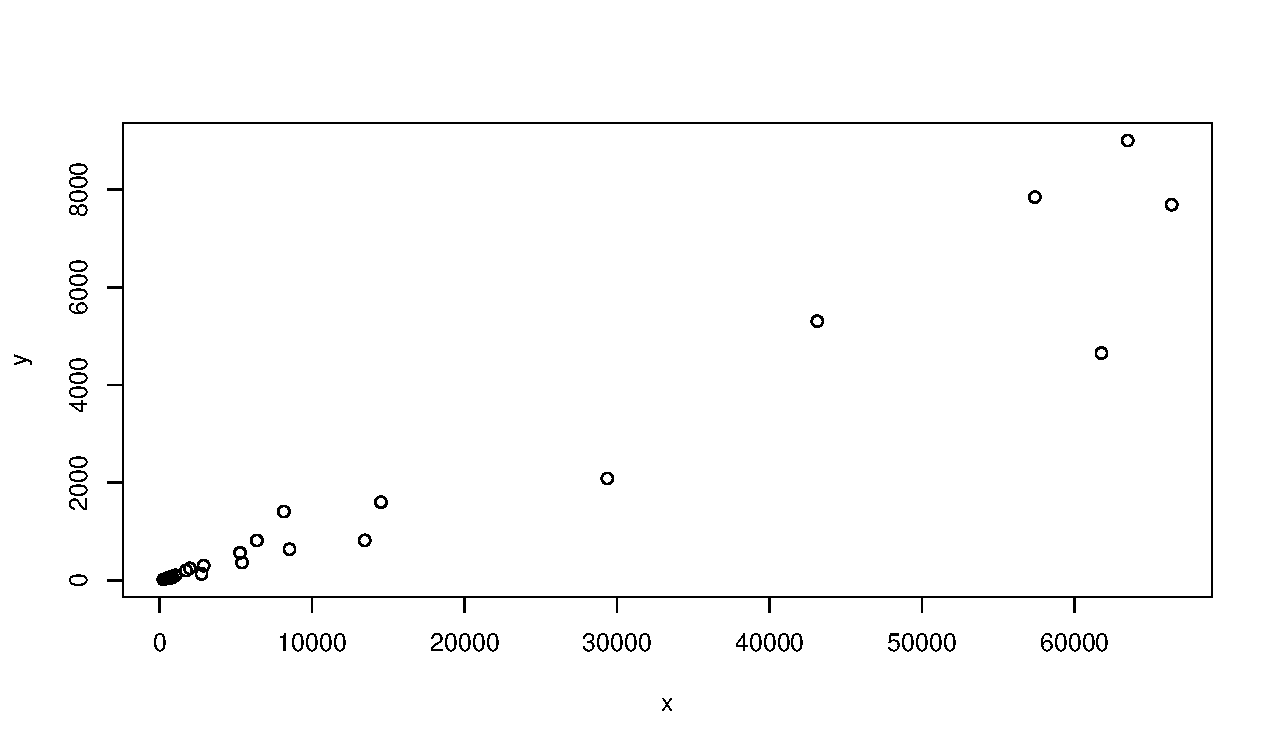
\includegraphics[width=\maxwidth]{figure/unnamed-chunk-12-1} 

}


\begin{kframe}\begin{alltt}
\hlcom{# Compute some common variables with common functions.}
\hlstd{r} \hlkwb{<-} \hlkwd{cor}\hlstd{(x, y)}
\hlstd{xbar} \hlkwb{<-} \hlkwd{mean}\hlstd{(x)}
\hlstd{ybar} \hlkwb{<-} \hlkwd{mean}\hlstd{(y)}
\hlkwd{cat}\hlstd{(}\hlstr{"r:"}\hlstd{, r,} \hlstr{"xbar:"}\hlstd{, xbar,} \hlstr{"ybar:"}\hlstd{, ybar)}
\end{alltt}
\begin{verbatim}
## r: 0.9635098 xbar: 16132.64 ybar: 1797.56
\end{verbatim}
\end{kframe}
\end{knitrout}

Therefore, $r=0.9635098$,
$\bar{x}=16132.64$, and $\bar{y}= 1797.56$.

\begin{knitrout}
\definecolor{shadecolor}{rgb}{0.969, 0.969, 0.969}\color{fgcolor}\begin{kframe}
\begin{alltt}
\hlcom{# Compute some common variables manually.}
\hlstd{Sxx} \hlkwb{<-} \hlkwd{sum}\hlstd{((x} \hlopt{-} \hlstd{xbar)} \hlopt{^} \hlnum{2}\hlstd{)}
\hlstd{Sxy} \hlkwb{<-} \hlkwd{sum}\hlstd{((x} \hlopt{-} \hlstd{xbar)} \hlopt{*} \hlstd{(y} \hlopt{-} \hlstd{ybar))}
\hlkwd{cat}\hlstd{(}\hlstr{"Sxx: "}\hlstd{, Sxx,} \hlstr{"Sxy: "}\hlstd{, Sxy)}
\end{alltt}
\begin{verbatim}
## Sxx:  12450023404 Sxy:  1453128337
\end{verbatim}
\end{kframe}
\end{knitrout}

Therefore, $S_{xx}=12450023404=1.245\times10^{10}$ and
$S_{xy}=1453128337=1.453\times 10^{9}$.

\begin{knitrout}
\definecolor{shadecolor}{rgb}{0.969, 0.969, 0.969}\color{fgcolor}\begin{kframe}
\begin{alltt}
\hlcom{# R's lm function fits linear models}
\hlstd{lm.1} \hlkwb{<-} \hlkwd{lm}\hlstd{(y} \hlopt{~} \hlstd{x)}
\hlkwd{summary}\hlstd{(lm.1)}
\end{alltt}
\begin{verbatim}
## 
## Call:
## lm(formula = y ~ x)
## 
## Residuals:
##      Min       1Q   Median       3Q      Max 
## -2470.81    -6.17    71.72   106.46  1677.32 
## 
## Coefficients:
##               Estimate Std. Error t value Pr(>|t|)    
## (Intercept) -85.391989 186.178031  -0.459    0.651    
## x             0.116717   0.006761  17.263 1.16e-14 ***
## ---
## Signif. codes:  0 '***' 0.001 '**' 0.01 '*' 0.05 '.' 0.1 ' ' 1
## 
## Residual standard error: 754.4 on 23 degrees of freedom
## Multiple R-squared:  0.9284,	Adjusted R-squared:  0.9252 
## F-statistic:   298 on 1 and 23 DF,  p-value: 1.164e-14
\end{verbatim}
\end{kframe}
\end{knitrout}

From the summary, we can see that
$\hat{\beta}_0=-85.391989$,
$\hat{\beta}_1=0.116717$,
$\Se*{\hat{\beta}_1}=0.006761$,
$t=17.263$, $p\text{-value}=1.64\times 10^{-14}$, and
$\hat{\sigma}=754.4$.


\begin{knitrout}
\definecolor{shadecolor}{rgb}{0.969, 0.969, 0.969}\color{fgcolor}\begin{kframe}
\begin{alltt}
\hlcom{# Sum Squared Fitted Values}
\hlkwd{sum}\hlstd{(lm.1}\hlopt{$}\hlstd{fitted.values} \hlopt{^} \hlnum{2}\hlstd{)}
\end{alltt}
\begin{verbatim}
## [1] 250385207
\end{verbatim}
\begin{alltt}
    \hlcom{# Sum Squared Residuals}
    \hlkwd{sum}\hlstd{(lm.1}\hlopt{$}\hlstd{residuals} \hlopt{^} \hlnum{2}\hlstd{)}
\end{alltt}
\begin{verbatim}
## [1] 13089860
\end{verbatim}
\end{kframe}
\end{knitrout}

Therefore, $\SS{\text{Res}}=\sum_{i=1}^n e_i^2=13089860=1.31\times10^7$.

\begin{knitrout}
\definecolor{shadecolor}{rgb}{0.969, 0.969, 0.969}\color{fgcolor}\begin{kframe}
\begin{alltt}
\hlcom{# Manual calculation of sigma^2 estimate}
\hlkwd{sum}\hlstd{(lm.1}\hlopt{$}\hlstd{residuals}\hlopt{^}\hlnum{2}\hlstd{)} \hlopt{/} \hlnum{23}
\end{alltt}
\begin{verbatim}
## [1] 569124.3
\end{verbatim}
\end{kframe}
\end{knitrout}

    Therefore, $\hat{\sigma}^2=69124.3=5.7\times 10^{5}$.

\begin{knitrout}
\definecolor{shadecolor}{rgb}{0.969, 0.969, 0.969}\color{fgcolor}\begin{kframe}
\begin{alltt}
\hlcom{# Manual calculation of sigma estimate}
\hlkwd{sqrt}\hlstd{(}\hlkwd{sum}\hlstd{(lm.1}\hlopt{$}\hlstd{residuals} \hlopt{^} \hlnum{2}\hlstd{)} \hlopt{/} \hlnum{23}\hlstd{)}
\end{alltt}
\begin{verbatim}
## [1] 754.4033
\end{verbatim}
\end{kframe}
\end{knitrout}

Therefore, $\hat{\sigma}= 754.4$.

\begin{knitrout}
\definecolor{shadecolor}{rgb}{0.969, 0.969, 0.969}\color{fgcolor}\begin{kframe}
\begin{alltt}
\hlcom{# t distribution values}
\hlkwd{qt}\hlstd{(}\hlnum{0.975}\hlstd{,} \hlnum{23}\hlstd{)}
\end{alltt}
\begin{verbatim}
## [1] 2.068658
\end{verbatim}
\end{kframe}
\end{knitrout}

Therefore, $c=2.07$.

\begin{knitrout}
\definecolor{shadecolor}{rgb}{0.969, 0.969, 0.969}\color{fgcolor}\begin{kframe}
\begin{alltt}
\hlcom{# 95% confidence interval}
\hlkwd{confint}\hlstd{(lm.1)}
\end{alltt}
\begin{verbatim}
##                    2.5 %      97.5 %
## (Intercept) -470.5305905 299.7466119
## x              0.1027305   0.1307034
\end{verbatim}
\begin{alltt}
\hlcom{# 95% prediction interval with predicted boxes if we had 10000 acres}
\hlkwd{predict}\hlstd{(lm.1,} \hlkwd{data.frame}\hlstd{(}\hlkwc{x} \hlstd{=} \hlnum{10000}\hlstd{),} \hlkwc{interval} \hlstd{=} \hlstr{"prediction"}\hlstd{)}
\end{alltt}
\begin{verbatim}
##        fit       lwr      upr
## 1 1081.777 -512.0407 2675.595
\end{verbatim}
\end{kframe}
\end{knitrout}

Q: Is $\sigma$ the same for all values of $y$?

A: It appears to not in the sense that the variance
appears to be higher with respect to higher acres.
Sigma will be smaller when there's less acres.
Later, this will be testing equal variance or homoscedastic
assumption. Later, when we talk about variable
transformations we can consider taking the logarithm.

Q: Are the error terms plausibly independent?
In other words,
does knowing one $e_i$ (residual) help predict $e_j$
(another residual) for a different county?

A: There's diagnostics for checking this. However,
intuitively there could be some common factors
at play when two counties are geographically close.
\chapter{C++}
\section{2020-01-21}
\subsection{Testing}
A pizza shop allows users to order pizza online and earn 10 points for each pizza
ordered.

Ordering: A user types \code{O} followed by a number N to order N pizzas.
e.g. \code{O} 2 orders 2 pizzas

The system allows ordering between 1 to 10 pizzas.
If \code{N} is outside this range, the system prints ``Illegal order.''

On a successful order, the system display ``2 pizzas ordered''
followed by the total number of points they have.

Redeeming: At any time, users can type \code{R} to try to redeem free pizza.
If the user has enough points(50), ``Free Pizza!'' is printed.
If the user does not have enough points, ``No pizza for you!''
is printed followed by the number of points the user has.

Points: At any time, users can type \code{P} to print their current points balance.

Write exhaustive tests for this system.

\textbf{Solution.}

\begin{itemize}
    \item \code{O 1} \textrightarrow{} 1 pizza ordered
    \item \code{O 10} \textrightarrow{} 10 pizzas ordered
    \item \code{O 0} \textrightarrow{} Illegal order
    \item \code{O 11} \textrightarrow{} Illegal order
    \item \code{1} \textrightarrow{} X
    \item \code{O 1 1} \textrightarrow{} X
    \item \code{O 5} \textrightarrow{} 5 pizzas ordered
          \begin{itemize}
              \item \code{P} \textrightarrow{} 50
              \item \code{R} \textrightarrow{} Free pizza!
              \item \code{P} \textrightarrow{} 0
          \end{itemize}
    \item \code{O 7} \textrightarrow{} 7 pizzas ordered
          \begin{itemize}
              \item \code{P} \textrightarrow{} 70
              \item \code{R} \textrightarrow{} Free pizza!
              \item \code{R} \textrightarrow{} No free pizza for you! 20
          \end{itemize}
\end{itemize}

\subsection{C++ Introduction}
\lstset{frame=tb,
    language=C++,
    aboveskip=3mm,
    belowskip=3mm,
    showstringspaces=false,
    columns=flexible,
    basicstyle={\ttfamily},
    numbers=none,
    numberstyle=\tiny\color{gray},
    keywordstyle=\color{RoyalBlue},
    commentstyle=\color{gray},
    stringstyle=\color{OrangeRed},
    breaklines=true,
    breakatwhitespace=true,
    tabsize=2
}
Simula 64 \textrightarrow{} first OO language (has classes)

C with classes \textrightarrow{} C++

History: C++99 \textrightarrow{} C++03 \textrightarrow{} C++11 \textrightarrow{} C++14

In C,
\begin{lstlisting}[language = C]
    # include <stdio.h>
    int main(void) {
        printf("Hello world\n");
        return 0;
    }
\end{lstlisting}
File: \code{hello.cc}
\begin{lstlisting}[language = C++]
    # include <iostream>
    using namespace std;

    int main() {
        cout << "Hello world" << endl;
        return 0;
    }
\end{lstlisting}

\subsection{iostream header}

\code{stdio.h}, \code{printf}, \code{scanf}, \code{read}
\textrightarrow{} not allowed in C++ (although valid)

Instead use, \code{std::cout <{}< data1 <{}< data2;}

By placing \code{using namespace std;}, we can say
\begin{itemize}
    \item \code{cout} instead of \code{std::cout}
    \item \code{endl} instead of \code{std::endl}
\end{itemize}

\subsection{Compile C++}
Since we created an alias for \code{g++} in assignment 0, we can instead
compile with simply \code{g++14 hello.cc}. To rename the output file
we can specify the \code{-o} parameter.
\begin{itemize}
    \item \code{g++ -std=c++14 hello.cc} \textrightarrow{} creates \code{a.out}
    \item \code{g++14 hello.cc -o prog.out} \textrightarrow{} creates \code{prog.out}
\end{itemize}

\subsection{Run C++}
\begin{itemize}
    \item \code{./a.out} \textrightarrow{} runs \code{a.out}
\end{itemize}

\subsection{C++ I/O}
\code{cout <{}< ``Hello'' <{}< ``World'' <{}< endl;}

When we create \code{iostream}, we get access to three stream variables.
\begin{enumerate}
    \item \code{stdin}
          \begin{itemize}
              \item \code{std::in}
              \item type: \code{istream}
              \item e.g. \code{cin <{}< x;}
          \end{itemize}
    \item \code{stdout}
          \begin{itemize}
              \item \code{std::out}
              \item type: \code{ostream}
              \item e.g. \code{cout <{}< ``Hello'';}
          \end{itemize}
    \item \code{stderr}
          \begin{itemize}
              \item \code{std::err}
              \item e.g. \code{cerr <{}< ``Error'';}
          \end{itemize}
\end{enumerate}

File: \code{add.cc}
\begin{lstlisting}[language = C++]
    #include <iostream>
    using namespace std;
    
    int main() {
      int x, y;
      cin >> x >> y;
      cout << x + y << endl;
    }
\end{lstlisting}
\begin{itemize}
    \item If a read fails, the expression \code{cin.fail()} is true
    \item If a read fails due to EOF, then expressions \code{cin.fail()}
          and \code{cin.eof()} are both true
\end{itemize}

File: \code{readInts.cc}
\begin{lstlisting}[language = C++]
    #include <iostream>
    using namespace std;
    
    int main() {
      int i;
      while (true) {
        cin >> i;
        if (cin.fail()) break;
        cout << i << endl;
      }
    }
\end{lstlisting}
\begin{itemize}
    \item Read as many \code{int}s from \code{stdin} and output to \code{stdout}
    \item Stop if a read fails
\end{itemize}

\begin{itemize}
    \item C++: an automatic conversion from iostream variables to bool.
    \item \code{cin} is true if \code{cin.fail()} is false
    \item \code{cin} is false if \code{cin.fail()} is true
\end{itemize}

\subsection{Summary of Files}
Files covered in this lecture found in \code{1201/lectures/c++}:
\begin{itemize}
    \item \code{hello.cc}
    \item \code{add.cc}
    \item \code{readInts.cc}
\end{itemize}

\makeheading{Lecture 6 | 2020-09-23}
Recall that last lecture, for a MLR,
we have $ \symbf{Y}=X\symbf{B}+\symbf{\varepsilon} $
with the assumption that $ \varepsilon\stackrel{\text{iid}}{\sim}N(0,\sigma^2) $.
Therefore, for a random vector $ \symbf{\varepsilon} $, we have
\[ \symbf{\varepsilon}\sim\text{MVN}
    \left( \begin{bmatrix}
            0      \\
            0      \\
            \vdots \\
            0      \\
            0
        \end{bmatrix},
    \begin{bmatrix}
            \sigma^2 & 0        & \cdots & 0        & 0        \\
            0        & \sigma^2 & \cdots & 0        & 0        \\
            \vdots   & \vdots   & \ddots & \vdots   & \vdots   \\
            0        & 0        & \cdots & \sigma^2 & 0        \\
            0        & 0        & \cdots & 0        & \sigma^2 \\
        \end{bmatrix} \right)=
    (\symbf{0}_{n\times 1},\sigma^2I_{n\times n}) \]
since $ \Cov{\varepsilon_1,\varepsilon_2}=0 $ due to independence.

Thus, $ \symbf{Y}\sim \text{MVN}(X\symbf{B},\sigma^2 I) $.
\begin{Definition}{Least squares for MLR}{}
    We define the \textbf{least squares for a multiple linear regression model}
    as
    \[ S(\beta_0,\beta_1,\ldots,\beta_p)
        =\sum\limits_{i=1}^{n}
        (y_i-(\Uunderbracket{
            \beta_0+\beta_1 x_{i1}+\cdots+\beta_p x_{ip}
        }_{\E{Y_i}=\mu_i}))^2
    \]
\end{Definition}
\begin{Theorem}{Least Square Estimates (LSEs) for MLR}{}
    Minimizing $ S(\beta_0,\beta_1,\ldots,\beta_p) $, gives the least squares
    estimate $ \hat{\symbf{\beta}}=(X^\top X)^{-1}X^\top\symbf{y} $.
\end{Theorem}
\begin{proof}
    The first partial is $ \frac{\partial S}{\partial \beta_0}=\sum\limits_{i=1}^{n} 2(y_i-\mu_u)(-1) $,
    and all other partials for $ j=1,\ldots,p $ are
    \[ \dfrac{\partial S}{\partial \beta_j}=
        \sum\limits_{i=1}^{n} 2(y_i-\mu_i)(-x_{ij}) \]
    Set $ \displaystyle \frac{\partial S}{\partial \beta_0}=0 $
    and $ \displaystyle \frac{\partial S}{\partial \beta_j}=0 $ for $ j=1,\ldots,p $
    to get
    \[ \begin{dcases}
            \sum\limits_{i=1}^{n} (y_i-\mu_i)=0\iff \symbf{1}_{n\times n}^\top(\symbf{y}-\symbf{\mu})=0 \\
            \sum\limits_{i=1}^{n} (y_i-\mu_i)x_{ij}=0\iff \symbf{x}_{j}^\top
            (\symbf{y}-\symbf{\mu})=0 & j=1,\ldots,p
        \end{dcases} \]
    since we recall that
    \[ X=\begin{bmatrix}
            1 & x_{11} & x_{12} & \cdots & x_{1p} \\
            \vdots                                \\
            1 & x_{n1} & x_{n2} & \cdots & x_{np}
        \end{bmatrix}=
        \begin{bmatrix}
            \symbf{1}_{n\times 1} & \symbf{x}_1 & \cdots & \symbf{x}_{p-1} & \symbf{x}_p
        \end{bmatrix} \]
    Therefore,
    \[ X^\top(\symbf{y}-X\symbf{B})=0\iff
        X^\top \symbf{y}-X^\top X\symbf{B}=0\iff
        X^\top X \symbf{B}=X^\top \symbf{y}\iff
        \symbf{B}=(X^\top X)^{-1}X^\top \symbf{y} \]
    assuming $ X^\top X $ is invertible (full rank of $ p+1 $ or linearly
    independent columns). So, the LS solution for $ \symbf{B} $ is given by
    $ \hat{\symbf{B}}=(X^\top X)^{-1}X^\top \symbf{y} $.
\end{proof}
\begin{Definition}{Residuals for MLR}{}
    The \textbf{residuals} for a multiple linear regression model is defined
    as
    \[ e_i=y_i-(\Uunderbracket{\hat{\beta}_0+\hat{\beta}_1x_{i1}+\cdots\hat{\beta}_p x_{ip}
        }_{\text{fitted value }\mu_i}) \]
    or equivalently, $ \hat{\symbf{\mu}}=X\hat{\symbf{B}} $ and
    $ \symbf{e}=\symbf{y}-\hat{\symbf{\mu}} $.
\end{Definition}
The estimate $ \sigma^2 $ based on $ e_i $'s is
\[ \hat{\sigma}^2=\frac{\Ss{\text{Res}}}{n-(p+1)}=
    \frac{\sum_{i=1}^{n} e_i^2}{n-p-1}=\frac{\symbf{e}^\top\symbf{e}}{n-p-1}  \]
since d.f.\ is $ n-(\text{no.\ estimated parameters}) $. When viewed
as a random variable,
\[ \frac{(n-p-1)\hat{\sigma}^2}{\sigma^2}\sim \chi^2(n-p-1)  \]
Inference for $ \hat{\symbf{\beta}}=(\hat{\beta}_0,\ldots,\hat{\beta}_p)^\top
    =(X^\top X)^{-1}X^\top \symbf{Y} $.

Note that $ \hat{\symbf{\beta}} $ is a matrix of constants and
$ \symbf{Y} $ is a random vector, and
$ \symbf{Y}\sim \text{MVN}(X\symbf{\beta},\sigma^2 I) $, so
\begin{align*}
    \E{\hat{\symbf{\beta}}}
     & =\E{(X^\top X)^{-1}X^\top \symbf{Y}}    \\
     & =(X^\top X)^{-1}X^\top\E{\symbf{Y}}     \\
     & =(X^\top X)^{-1}(X^\top X)\symbf{\beta} \\
     & =\symbf{\beta}
\end{align*}
That is, $ \E{\hat{\beta}_0},\ldots,\E{\hat{\beta}_p}=\beta_p $
all unbiased.
\begin{align*}
    \Var{(X^\top X)^{-1}X^\top\symbf{Y}}
     & =(X^\top X)^{-1}X^{\top}\Var{\symbf{Y}}\left[ (X^\top X)^{-1}X^\top \right]^\top                              \\
     & =(X^\top X)^{-1}X^\top \sigma^2 I(X^\top)^\top\left[ (X^\top X)^{-1} \right]^\top & X^\top X\text{ symmetric} \\
     & =\sigma^2(X^\top X)^{-1}(X^\top X)(X^\top X)^{-1}
\end{align*}
Since $ \hat{\symbf{\beta}} $ is a linear transformation of $ \symbf{Y} $
we have
$ \hat{\symbf{\beta}} \sim \text{MVN}(\symbf{\beta},\sigma^2
    \Uunderbracket{(X^\top X)^{-1}}_{V}) $. We proved the following theorem.
\begin{Theorem}{Distribution of $ \hat{\beta}_j $}{}
    The distribution of a given $ \hat{\beta}_j $ is
    \[ \hat{\beta}_j \sim N(\beta_j,\sigma^2 V_{jj}) \]
\end{Theorem}
from marginal property of MVN.\
\[ \frac{\hat{\beta}_j-\beta_j}{\sigma\sqrt{V_{jj}}} \sim N(0,1)  \]
\[ \frac{\hat{\beta}_j-\beta_j}{\hat{\sigma}\sqrt{V_{jj}}} \sim t(n-p-1)  \]
\begin{Definition}{Standard error for $ \hat{\beta}_j $}{}
    We define the \textbf{standard error} of $ \hat{\beta}_j $ as
    \[ \Se{\hat{\beta}_j}=\hat{\sigma}\sqrt{V_{jj}} \]
\end{Definition}
So, a $ (1-\alpha) $ confidence interval for $ \beta_j $
is
\[ \hat{\beta}_j\pm c\Se{\hat{\beta}_j} \]
where $ c $ is $ (1-(\alpha/2)) $ quantile of $ t(n-p-1) $.

To test $ H_0 $: $ \beta_j=0 $ vs $ H_A $: $ \beta_j\neq 0 $,
calculate $ t $-statistic
$ t=\dfrac{\hat{\beta}_j}{\Se{\hat{\beta}_j}} $
reject at level $ \alpha $ if $ \abs{t}>c $ and
$ p $-value is $ 2P(T\geqslant \abs{t}) $ where $ T \sim t(n-p-1) $.

Interpretation of $ \hat{\symbf{\beta}} $: fitted linear
regression model says $ \widehat{\E{Y}} $
(estimate of the expected response) is
$ \hat{\beta}_0+\hat{\beta}_1x_1+\cdots+\hat{\beta}_p x_p $.
\begin{itemize}
    \item $ \hat{\beta}_0 $ is the estimate of expected response
          when all explanatory variables are equal to 0.
    \item $ \hat{\beta}_j $ is the estimated change
          in expected response for a unit increase in $ x_j $,
          when holding all other explanatory variables constant,
          e.g.\
          \[ \hat{\beta}_0+\hat{\beta}_1(x_1+1)+\cdots+\hat{\beta}_p x_p
              -(\hat{\beta}_0+\hat{\beta}_1 x_1+\cdots+\hat{\beta}_p x_p)=\hat{\beta}_1 \]
\end{itemize}

\begin{Remark}{}{}
    When it's written $ V_{jj} $, that means the $ j+1^{\text{th}} $
    column and $ j+1^{\text{th}} $ row since we start from index $ 0 $
    for these matrices. Some unfortunate events may have happened
    on the quiz to me due to this.
\end{Remark}

\begin{Example}{Rocket MLR}{}
    Let $ n=12 $, $ \hat{\symbf{\beta}}=(473.6, 16.7,-1.09)^\top
        =(\hat{\beta}_0,\hat{\beta}_1,\hat{\beta}_2)^\top $.
    \begin{itemize}
        \item $ x_1 $: nozzle area ($ 1 = L,0=S $)
        \item $ x_2 $: propellant ratio
        \item $ Y $: thrust
    \end{itemize}
    \[ \hat{\sigma}=\sqrt{\frac{\sum\limits_{i=1}^{12} e_i^2}{12-1-2}}=
        \sqrt{\frac{\symbf{e}^\top \symbf{e}}{9}}=
        2.655 \]
    Interpretation of $ \hat{\symbf{\beta}} $:
    \begin{itemize}
        \item $ \hat{\beta}_1 $ estimated change in expected thrust is 16.7
              when changing small to large nozzle while holding other variables
              (propellant ratio) constant.
        \item $ \hat{\beta}_2 $ estimated thrust to decrease by 1.09 on average
              for a unit increase in propellant ratio while holding other
              variables (nozzle area) constant.
    \end{itemize}
    Given $ \Se{\hat{\beta}_2}=0.94 $,
    we compute the $ t $-statistic for $ H_0 $: $ \beta_2=0 $ vs $ H_A $: $ \beta_2\neq 0 $
    which is $ t=-1.09/0.94=-1.16 $.
    \[ p\text{-value}=2P(T\geqslant 1.16)=0.275\text{ from R where } T \sim t(9)\]
    Do not reject $ H_0 $ (e.g. $ \alpha=0.05 $), therefore
    propellent ratio does not significantly influence thrust.
\end{Example}

\makeheading{Lecture 7 | 2020-09-28}
Recall:
\[ \symbf{Y}=X\symbf{\beta}+\symbf{\varepsilon}
    \sim \text{MVN}(X\symbf{\beta},\sigma^2 I) \]
\begin{itemize}
    \item Estimates: $ \hat{\symbf{\beta}}=(X^\top X)^{-1}X^\top \symbf{Y} $
    \item Fitted values: $ \hat{\symbf{\mu}}=X\hat{\symbf{\beta}} $
    \item Residuals: $ \symbf{e}=\symbf{y}-\hat{\symbf{\mu}} $
\end{itemize}
Geometric interpretation of data.
Constants: $ X=\begin{bmatrix}
        \symbf{1} & \symbf{x}_1 & \cdots & \symbf{x}_p
    \end{bmatrix}_{n\times(p+1)} $

Values of responses: $
    \symbf{y}=\begin{bmatrix}
        y_1    \\
        y_2    \\
        \vdots \\
        y_n
    \end{bmatrix}\in\mathbb{R}^n $

Recall: $ \text{Span}(X)=
    \set{b_0\symbf{1}+b_1\symbf{x}_1+\cdots+b_p\symbf{x}_p:b_0,\ldots,b_p\in\mathbb{R}}
    \subset \mathbb{R}^n $
which is all linear combinations of columns of $ X $ which is a subspace
of $ \mathbb{R}^n $. Recall, by assumption
$ \rank(X)=p+1 $.

We can say $ \text{Span}(X) $ represents all possible vector
values $ X\symbf{b} $ where $ \symbf{b}=(b_0,b_1,\ldots,b_p)^\top $.

Generally, $ \symbf{y}\notin\text{Span}(X) $, so since
the linear model is an approximation, $ \symbf{\varepsilon} $
variability not explained by model.

Intuitively, it makes sense to choose an estimate
$ \hat{\symbf{\beta}} $ so that $ X\hat{\symbf{\beta}} $
is as close to $ \symbf{y} $ as possible. Therefore,
$ \symbf{e} $ must be orthogonal to $ \text{Span}(X)
    \iff \symbf{e} $ is orthogonal to all columns of $ X $.
\begin{align*}
    \symbf{1}^\top\cdot(\symbf{y}-\hat{\symbf{\mu}})   & =      0 \\
    \symbf{x}_1^\top\cdot(\symbf{y}-\hat{\symbf{\mu}}) & =      0 \\
    \vdots                                                        \\
    \symbf{x}_p^\top\cdot(\symbf{y}-\hat{\symbf{\mu}}) & =      0
\end{align*}
which is the same as LS estimates.

\[ \hat{\symbf{\mu}}=X\hat{\symbf{\beta}},
    \quad \symbf{e}=\symbf{y}-\hat{\symbf{\mu}} \]
Define the \textbf{hat matrix} as
\[ H=X(X^\top X)^{-1}X^{\top} \]
Properties of $ H $
\begin{enumerate}[label=(\arabic*)]
    \item $ H $ is symmetric.
    \item $ H $ is idempotent.
    \item $ I-H $ is symmetric idempotent.
\end{enumerate}
\[ H^\top=[X(X^\top X)^{-1}X^\top]^\top=X(X^\top X)^{-1}X^\top=H \]
\[ HH=X(X^\top X)^{-1}(X^\top X)(X^\top X)^{-1}X^\top=H \]

Let's view $ \hat{\symbf{\mu}} $ and $ \symbf{e} $
as random vectors
\[ \hat{\symbf{\mu}}=X\hat{\symbf{\beta}}=
    X(X^\top X)^{-1}X^\top \symbf{Y}=H\symbf{Y} \]
\[ \symbf{e}=\symbf{Y}-\hat{\symbf{\mu}}=I\symbf{Y}-H\symbf{Y}=
    (I-H)\symbf{Y} \]
\[ \E{\hat{\symbf{\mu}}}=\E{H\symbf{Y}}=H\E{\symbf{Y}}=
    X(X^\top X)^{-1}X^\top \Uunderbracket{X\symbf{\beta}}_{\E{\symbf{Y}}}
    =X\symbf{\beta}
\]
\[ \Var{\hat{\symbf{\mu}}}=\Var{H\symbf{Y}}=
    H\Var{\symbf{Y}}H^\top=H\sigma^2I H^\top=\sigma^2(HH^\top)=\sigma^2H \]
\[ \E{ \symbf{e}}=
    \E{(I-H)\symbf{Y}}=\E{\symbf{Y}}-\E{H\symbf{Y}}=X\symbf{\beta}-X\symbf{\beta}=0 \]
\[ \Var{\symbf{e}}=
    (I-H)\Var{\symbf{Y}}(I-H)^\top=\sigma^2(I-H)(I-H)^\top=\sigma^2(I-H) \]
So since $ \hat{\symbf{\mu}} $ and $ \symbf{e} $
are linear transformations of $ \symbf{Y} $
\[ \hat{\symbf{\mu}}\sim\text{MVN}(X\symbf{\beta},\sigma^2 H) \]
\[ \hat{\symbf{e}}\sim\text{MVN}(0,\sigma^2(I-H)) \]
Prediction: Suppose we want to predict response for
(the first 1 represents the intercept)
\[ \symbf{x}_0=\begin{bmatrix}
        1 & x_{01} & x_{02} & \cdots & x_{0p}
    \end{bmatrix}_{1\times (p+1)} \]
Let $ Y_0 $ random variable representing the response
associated with $ \symbf{x}_0 $. The MLR says
\[ Y_0 \sim N(\beta_0+\beta_1x_{01}+\cdots+\beta_p x_{0p},\sigma^2) \]
So we predict the value
\[ \hat{y}_0=\hat{\beta}_0+\hat{\beta}_1x_{01}+\cdots+
    \hat{\beta}_p x_{0p}=\symbf{x}_0\hat{\symbf{\beta}} \]
which represents the estimated mean response given
$ x_{01},x_{02},\ldots,x_{0p} $. Corresponding distribution
has
\[ \E{\hat{Y}_0}=\symbf{x}_0\E{\hat{\symbf{\beta}}}=\symbf{x}_0\symbf{\beta}
    =\E{Y_0} \]
\[ \Var{\hat{Y}_0}=\symbf{x}_0\Var{\hat{\symbf{\beta}}}\symbf{x}_0^\top=
    \symbf{x}_0\sigma^2(X^\top X)^{-1}\symbf{x}_0^\top \]
Therefore,
\[ \hat{Y}_0 \sim N(\symbf{x}_0\symbf{\beta},\sigma^2\symbf{x}_0(X^\top X)^{-1}
    \symbf{x}_0^\top) \]
\[ \frac{\hat{Y}_0-\symbf{x}_0\symbf{\beta}}{\sigma\sqrt{
            \symbf{x}_0(X^\top X)^{-1}\symbf{x}_0^\top
        }}\sim N(0,1)  \]

\[ \frac{\hat{Y}_0-\symbf{x}_0\symbf{\beta}}{\hat{\sigma}\sqrt{
            \symbf{x}_0(X^\top X)^{-1}\symbf{x}_0^\top
        }}\sim t(n-(p+1))=t(n-p-1)  \]
A $ (1-\alpha) $ confidence interval for the mean
response given $ \symbf{x}_0 $,
\[ \hat{y}_0\pm c \hat{\sigma}\sqrt{
        \symbf{x}_0(X^\top X)^{-1}\symbf{x}_0^\top} \]
where $ c $ is the $ 1-\alpha/2 $ quantile of $ t(n-p-1) $.

Prediction error: $ Y_0-\hat{Y}_0 $ which are independent
since $ Y_0 $ is a random variable with variance $ \sigma^2 $
and $ \hat{Y}_0 $ is a function of $ Y_1,\ldots,Y_n $. Therefore,
\[ \E{Y_0-\hat{Y}_0}=\symbf{x}_0\symbf{\beta}-\symbf{x}_0\symbf{\beta}=0 \]
\[ \Var{Y_0-\hat{Y}_0}=\Var{Y_0}+(-1)^2\Var{\hat{Y}_0}=
    \sigma^2+\sigma^2(\symbf{x}_0(X^\top X)^{-1}\symbf{x}_0^\top) \]
Therefore,
\[ Y_0-\hat{Y}_0 \sim N(
    0,\sigma^2(1+\symbf{x}_0(X^\top X)^{-1}\symbf{x}_0^\top)
    ) \]
A $ (1-\alpha) $ prediction interval for $ y_0 $
\[ \hat{y}_0\pm c\hat{\sigma}\sqrt{1+\symbf{x}_0(X^\top X)^{-1}\symbf{x}_0^\top} \]
where $ c $ is the $ 1-\alpha/2 $ quantile of $ t(n-p-1) $.

Intuition: prediction interval wider than CI for mean. Estimating
an average is ``easier'' than an individual response.


\makeheading{Lecture 8 | 2020-09-30}
\section{Categorical Predictors}
\subsection{R Demo}
\begin{knitrout}
\definecolor{shadecolor}{rgb}{0.969, 0.969, 0.969}\color{fgcolor}\begin{kframe}
\begin{alltt}
\hlcom{## NASA rocket data example}

\hlcom{## From: R.S. Jankovsky, T.D. Smith, A.J. Pavli (1999). "High-Area-Ratio Rocket}
\hlcom{## Nozzle at High Combustion Chamber Pressure-Experimental and Analytical}
\hlcom{## Validation".}

\hlcom{# setwd(...) first if your CSV file is somewhere else}
\hlstd{rocket} \hlkwb{<-} \hlkwd{read.csv}\hlstd{(}\hlstr{"csv/rocket.csv"}\hlstd{)}
\hlcom{# output all data in rocket vector}
\hlstd{rocket}
\end{alltt}
\begin{verbatim}
##    thrust nozzle propratio
## 1   488.0      1      3.97
## 2   481.6      1      5.91
## 3   485.9      1      4.98
## 4   486.0      1      4.91
## 5   484.5      1      3.89
## 6   483.8      1      5.80
## 7   463.2      0      5.99
## 8   471.2      0      4.95
## 9   469.5      0      3.91
## 10  470.5      0      5.85
## 11  469.5      0      4.71
## 12  465.7      0      3.84
\end{verbatim}
\end{kframe}
\end{knitrout}

$Y$ (thrust) is the response variable, and there
are two explanatory variables $x_1,x_2$
(nozzle, propratio) where nozzle is coded
as 1 if it's large.

\begin{knitrout}
\definecolor{shadecolor}{rgb}{0.969, 0.969, 0.969}\color{fgcolor}\begin{kframe}
\begin{alltt}
\hlcom{# Scatter plots where mfrow is used to put multiple plots on one image}
\hlkwd{par}\hlstd{(}\hlkwc{mfrow} \hlstd{=} \hlkwd{c}\hlstd{(}\hlnum{1}\hlstd{,} \hlnum{2}\hlstd{))}
\hlkwd{plot}\hlstd{(rocket}\hlopt{$}\hlstd{nozzle,}
  \hlstd{rocket}\hlopt{$}\hlstd{thrust,}
\hlkwc{ylab} \hlstd{=} \hlstr{"Thrust"}\hlstd{,}
\hlkwc{xlab} \hlstd{=} \hlstr{"Nozzle size (1 = large)"}\hlstd{)}
\hlkwd{plot}\hlstd{(rocket}\hlopt{$}\hlstd{propratio,}
  \hlstd{rocket}\hlopt{$}\hlstd{thrust,}
\hlkwc{ylab} \hlstd{=} \hlstr{"Thrust"}\hlstd{,}
\hlkwc{xlab} \hlstd{=} \hlstr{"Propellant to fuel ratio"}\hlstd{)}
\end{alltt}
\end{kframe}

{\centering 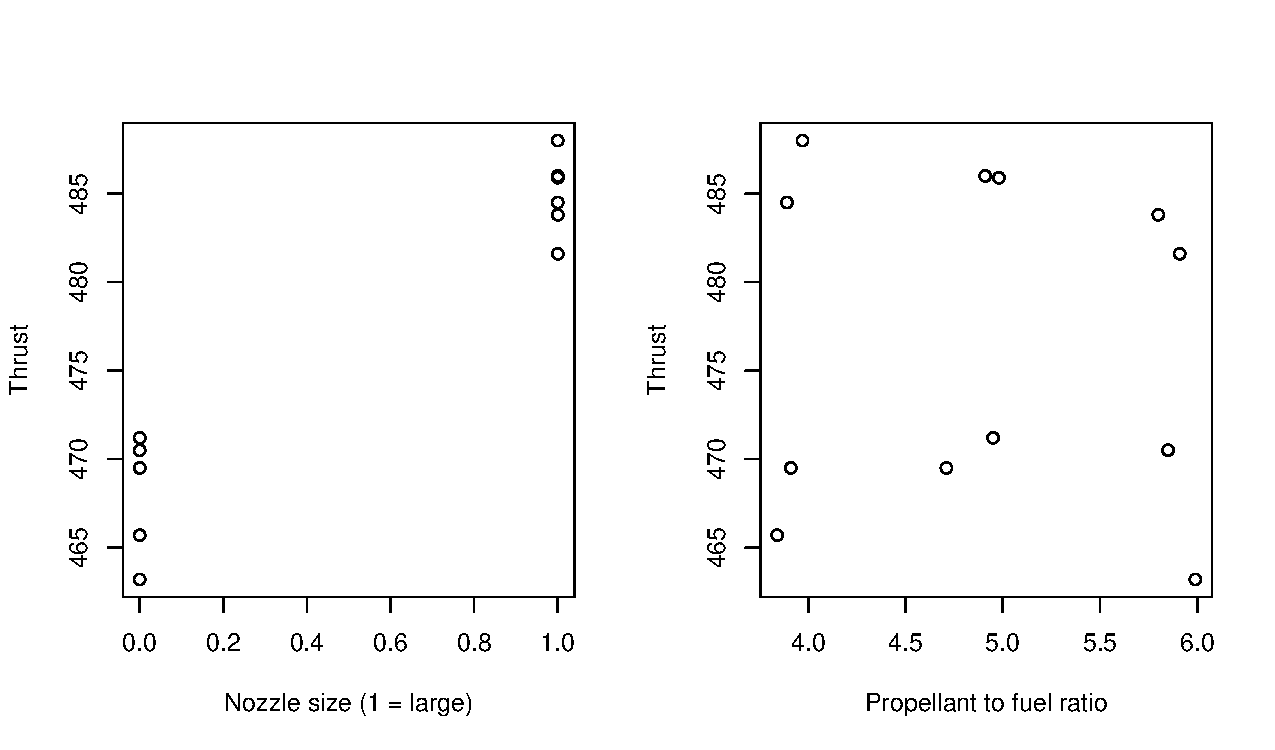
\includegraphics[width=\maxwidth]{figure/unnamed-chunk-21-1} 

}


\end{knitrout}

Left is nozzle size vs thrust. Right is propellant
relationship vs thrust.

\begin{knitrout}
\definecolor{shadecolor}{rgb}{0.969, 0.969, 0.969}\color{fgcolor}\begin{kframe}
\begin{alltt}
\hlcom{# Fit MLR using lm}
\hlstd{m1} \hlkwb{<-} \hlkwd{lm}\hlstd{(thrust} \hlopt{~} \hlstd{nozzle} \hlopt{+} \hlstd{propratio,} \hlkwc{data} \hlstd{= rocket)}
\hlkwd{summary}\hlstd{(m1)}
\end{alltt}
\begin{verbatim}
## 
## Call:
## lm(formula = thrust ~ nozzle + propratio, data = rocket)
## 
## Residuals:
##     Min      1Q  Median      3Q     Max 
## -3.8459 -1.7555  0.5934  1.2906  3.3008 
## 
## Coefficients:
##             Estimate Std. Error t value Pr(>|t|)    
## (Intercept) 473.6039     4.7158 100.430 4.88e-15 ***
## nozzle       16.7383     1.5329  10.919 1.71e-06 ***
## propratio    -1.0948     0.9414  -1.163    0.275    
## ---
## Signif. codes:  0 '***' 0.001 '**' 0.01 '*' 0.05 '.' 0.1 ' ' 1
## 
## Residual standard error: 2.655 on 9 degrees of freedom
## Multiple R-squared:  0.9303,	Adjusted R-squared:  0.9148 
## F-statistic: 60.05 on 2 and 9 DF,  p-value: 6.238e-06
\end{verbatim}
\begin{alltt}
\hlstd{m2} \hlkwb{<-} \hlkwd{lm}\hlstd{(thrust} \hlopt{~} \hlnum{0} \hlopt{+} \hlstd{nozzle,} \hlkwc{data} \hlstd{= rocket)}
\hlkwd{summary}\hlstd{(m2)}
\end{alltt}
\begin{verbatim}
## 
## Call:
## lm(formula = thrust ~ 0 + nozzle, data = rocket)
## 
## Residuals:
##    Min     1Q Median     3Q    Max 
##  -3.37   0.58 233.12 469.50 471.20 
## 
## Coefficients:
##        Estimate Std. Error t value Pr(>|t|)   
## nozzle    485.0      141.2   3.435  0.00558 **
## ---
## Signif. codes:  0 '***' 0.001 '**' 0.01 '*' 0.05 '.' 0.1 ' ' 1
## 
## Residual standard error: 345.8 on 11 degrees of freedom
## Multiple R-squared:  0.5175,	Adjusted R-squared:  0.4736 
## F-statistic:  11.8 on 1 and 11 DF,  p-value: 0.005575
\end{verbatim}
\begin{alltt}
\hlkwd{anova}\hlstd{(m1)}
\end{alltt}
\begin{verbatim}
## Analysis of Variance Table
## 
## Response: thrust
##           Df Sum Sq Mean Sq  F value    Pr(>F)    
## nozzle     1 836.67  836.67 118.7377 1.743e-06 ***
## propratio  1   9.53    9.53   1.3524    0.2748    
## Residuals  9  63.42    7.05                       
## ---
## Signif. codes:  0 '***' 0.001 '**' 0.01 '*' 0.05 '.' 0.1 ' ' 1
\end{verbatim}
\end{kframe}
\end{knitrout}

On the left it's $Y$ (response variable) and on the
right it's $x_1,x_2$ (explanatory variables).
From summary, we get the estimate vector
$\hat{\symbf{\beta}}=(473.6039, 16.7383,-1.0948)^\top$.

\begin{knitrout}
\definecolor{shadecolor}{rgb}{0.969, 0.969, 0.969}\color{fgcolor}\begin{kframe}
\begin{alltt}
\hlcom{# Manual beta estimates where rep is used to make the columns of 1s}
\hlstd{X} \hlkwb{<-} \hlkwd{cbind}\hlstd{(}\hlkwd{rep}\hlstd{(}\hlnum{1}\hlstd{,} \hlnum{12}\hlstd{), rocket}\hlopt{$}\hlstd{nozzle, rocket}\hlopt{$}\hlstd{propratio)} \hlcom{# X matrix}
\hlstd{y} \hlkwb{<-} \hlkwd{matrix}\hlstd{(rocket}\hlopt{$}\hlstd{thrust,} \hlkwc{ncol} \hlstd{=} \hlnum{1}\hlstd{)} \hlcom{# response vector}
  \hlstd{beta_hat} \hlkwb{<-} \hlkwd{solve}\hlstd{(}\hlkwd{t}\hlstd{(X)} \hlopt \hlstd{X)} \hlopt \hlkwd{t}\hlstd{(X)} \hlopt \hlstd{y}
  \hlstd{beta_hat}
\end{alltt}
\begin{verbatim}
##            [,1]
## [1,] 473.603924
## [2,]  16.738319
## [3,]  -1.094822
\end{verbatim}
\end{kframe}
\end{knitrout}

  \code{solve} is used for the inverse. \code{\%*\%} is used
  for matrix-matrix multiplication, and \code{t(X)}
  is used for transposing $X$.

\begin{knitrout}
\definecolor{shadecolor}{rgb}{0.969, 0.969, 0.969}\color{fgcolor}\begin{kframe}
\begin{alltt}
\hlcom{# Manual sigma estimate}
\hlstd{mu_hat} \hlkwb{<-} \hlstd{X} \hlopt \hlstd{beta_hat} \hlcom{# fitted values}
\hlstd{e} \hlkwb{<-} \hlstd{y} \hlopt{-} \hlstd{mu_hat} \hlcom{# residuals}
\hlstd{sigma_hat} \hlkwb{<-} \hlkwd{sqrt}\hlstd{((}\hlkwd{t}\hlstd{(e)} \hlopt \hlstd{e)} \hlopt{/} \hlnum{9}\hlstd{)} \hlcom{# Note n-p-1 = 12-2-1 = 9}
\hlstd{sigma_hat}
\end{alltt}
\begin{verbatim}
##        [,1]
## [1,] 2.6545
\end{verbatim}
\begin{alltt}
\hlstd{sigma_hat} \hlkwb{<-} \hlkwd{sqrt}\hlstd{(}\hlkwd{sum}\hlstd{(e} \hlopt{^} \hlnum{2}\hlstd{)} \hlopt{/} \hlnum{9}\hlstd{)} \hlcom{# equivalent}
\hlstd{sigma_hat}
\end{alltt}
\begin{verbatim}
## [1] 2.6545
\end{verbatim}
\end{kframe}
\end{knitrout}
  \begin{itemize}
    \item $\hat{\symbf{\mu}}=X\hat{\symbf{\beta}}$
    \item $\symbf{e}=\symbf{y}-\hat{\symbf{\mu}}$
    \item $\hat{\sigma}=\sqrt{\biggl(\sum_{i=1}^{n}e_i^2\biggr)/9}=2.6545$, or
    \item $\hat{\sigma}=\sqrt{(\symbf{e}^\top\symbf{e})/9}=2.6545$
  \end{itemize}
\begin{knitrout}
\definecolor{shadecolor}{rgb}{0.969, 0.969, 0.969}\color{fgcolor}\begin{kframe}
\begin{alltt}
\hlcom{# Covariance matrix of beta_hat}
\hlkwd{vcov}\hlstd{(m1)}
\end{alltt}
\begin{verbatim}
##             (Intercept)      nozzle   propratio
## (Intercept)   22.238325 -1.02316688 -4.32080608
## nozzle        -1.023167  2.34987593 -0.03102117
## propratio     -4.320806 -0.03102117  0.88631920
\end{verbatim}
\begin{alltt}
\hlkwd{sqrt}\hlstd{(}\hlkwd{diag}\hlstd{(}\hlkwd{vcov}\hlstd{(m1)))} \hlcom{# SEs of individual betas}
\end{alltt}
\begin{verbatim}
## (Intercept)      nozzle   propratio 
##   4.7157528   1.5329305   0.9414453
\end{verbatim}
\begin{alltt}
\hlcom{# Manual}
\hlstd{se_beta} \hlkwb{<-} \hlstd{sigma_hat} \hlopt{*} \hlkwd{sqrt}\hlstd{(}\hlkwd{diag}\hlstd{(}\hlkwd{solve}\hlstd{(}\hlkwd{t}\hlstd{(X)} \hlopt \hlstd{X)))}
\hlstd{se_beta}
\end{alltt}
\begin{verbatim}
## [1] 4.7157528 1.5329305 0.9414453
\end{verbatim}
\end{kframe}
\end{knitrout}

  \begin{itemize}
    \item $\Se*{\hat{\symbf{\beta}}}=\hat{\sigma}\sqrt{(X^\top X)^{-1}}=(4.71, 1.53, 0.94)^{\top}$
  \end{itemize}

\begin{knitrout}
\definecolor{shadecolor}{rgb}{0.969, 0.969, 0.969}\color{fgcolor}\begin{kframe}
\begin{alltt}
\hlcom{# Estimate the mean response for units with small nozzle and propellant ratio 5.5}
\hlcom{# include a 95% CI}
\hlkwd{predict}\hlstd{(}
\hlkwc{object} \hlstd{= m1,}
\hlkwc{newdata} \hlstd{=} \hlkwd{data.frame}\hlstd{(}\hlkwc{nozzle} \hlstd{=} \hlnum{0}\hlstd{,} \hlkwc{propratio} \hlstd{=} \hlnum{5.5}\hlstd{),}
\hlkwc{interval} \hlstd{=} \hlstr{"confidence"}\hlstd{,}
\hlkwc{level} \hlstd{=} \hlnum{0.95}
\hlstd{)}
\end{alltt}
\begin{verbatim}
##        fit      lwr      upr
## 1 467.5824 464.7929 470.3719
\end{verbatim}
\end{kframe}
\end{knitrout}

  Therefore, $\hat{y}_0=467.58$. The 95\% confidence interval for the mean
  response given $\symbf{x}_0$ is $[464.7929,470.3719]$.

\begin{knitrout}
\definecolor{shadecolor}{rgb}{0.969, 0.969, 0.969}\color{fgcolor}\begin{kframe}
\begin{alltt}
\hlcom{# Manual calculation}
\hlstd{x0} \hlkwb{<-} \hlkwd{matrix}\hlstd{(}\hlkwd{c}\hlstd{(}\hlnum{1}\hlstd{,} \hlnum{0}\hlstd{,} \hlnum{5.5}\hlstd{),} \hlkwc{nrow} \hlstd{=} \hlnum{1}\hlstd{)}
\hlstd{y0_hat} \hlkwb{<-} \hlstd{x0} \hlopt \hlstd{beta_hat}
\hlstd{y0_hat}
\end{alltt}
\begin{verbatim}
##          [,1]
## [1,] 467.5824
\end{verbatim}
\begin{alltt}
\hlcom{# mu0 is also known as \textbackslash{}hat\{Y\}_0}
\hlstd{se_mu0} \hlkwb{<-} \hlstd{sigma_hat} \hlopt{*} \hlkwd{sqrt}\hlstd{(x0} \hlopt \hlkwd{solve}\hlstd{(}\hlkwd{t}\hlstd{(X)} \hlopt \hlstd{X)} \hlopt \hlkwd{t}\hlstd{(x0))}
\hlstd{se_mu0}
\end{alltt}
\begin{verbatim}
##          [,1]
## [1,] 1.233132
\end{verbatim}
\begin{alltt}
\hlstd{crit_val} \hlkwb{<-} \hlkwd{qt}\hlstd{(}\hlnum{0.975}\hlstd{,} \hlnum{9}\hlstd{)}
\hlstd{ci_lo} \hlkwb{<-} \hlstd{y0_hat} \hlopt{-} \hlstd{crit_val} \hlopt{*} \hlstd{se_mu0}
\hlstd{ci_hi} \hlkwb{<-} \hlstd{y0_hat} \hlopt{+} \hlstd{crit_val} \hlopt{*} \hlstd{se_mu0}
\hlkwd{c}\hlstd{(y0_hat, ci_lo, ci_hi)}
\end{alltt}
\begin{verbatim}
## [1] 467.5824 464.7929 470.3719
\end{verbatim}
\end{kframe}
\end{knitrout}

  \begin{itemize}
    \item $\symbf{x}_0=\begin{bmatrix}1&0&5.5\end{bmatrix}$
    \item $\hat{y}_0=\symbf{x}_0\hat{\symbf{\beta}}=467.5824$
    \item $\Se*{\hat{Y}_0}=\hat{\sigma}\sqrt{\symbf{x}_0(X^\top X)^{-1}\symbf{x}_0^\top}=
            1.233132$
  \end{itemize}
  Therefore, $\hat{y}_0=467.58$. The 95\% confidence interval for the mean
  response given $\symbf{x}_0$ is $[464.7929,470.3719]$.

\begin{knitrout}
\definecolor{shadecolor}{rgb}{0.969, 0.969, 0.969}\color{fgcolor}\begin{kframe}
\begin{alltt}
\hlcom{# Predict the value of the response for a unit with small nozzle and propellant ratio 5.5}
\hlcom{# include a 95% PI}
\hlkwd{predict}\hlstd{(}
\hlkwc{object} \hlstd{= m1,}
\hlkwc{newdata} \hlstd{=} \hlkwd{data.frame}\hlstd{(}\hlkwc{nozzle} \hlstd{=} \hlnum{0}\hlstd{,} \hlkwc{propratio} \hlstd{=} \hlnum{5.5}\hlstd{),}
\hlkwc{interval} \hlstd{=} \hlstr{"prediction"}\hlstd{,}
\hlkwc{level} \hlstd{=} \hlnum{0.95}
\hlstd{)}
\end{alltt}
\begin{verbatim}
##        fit      lwr      upr
## 1 467.5824 460.9612 474.2036
\end{verbatim}
\end{kframe}
\end{knitrout}

  Therefore, $y_0=467.5824$. The 95\% prediction interval for the
  response $(y_0)$ given $\symbf{x}_0$ is $[460.9612, 474.2036]$.

\begin{knitrout}
\definecolor{shadecolor}{rgb}{0.969, 0.969, 0.969}\color{fgcolor}\begin{kframe}
\begin{alltt}
\hlcom{# Manual calculation for an individual}
\hlstd{x0} \hlkwb{<-} \hlkwd{matrix}\hlstd{(}\hlkwd{c}\hlstd{(}\hlnum{1}\hlstd{,} \hlnum{0}\hlstd{,} \hlnum{5.5}\hlstd{),} \hlkwc{nrow} \hlstd{=} \hlnum{1}\hlstd{)}
\hlstd{y0_hat} \hlkwb{<-} \hlstd{x0} \hlopt \hlstd{beta_hat}
\hlstd{se_y0} \hlkwb{<-} \hlstd{sigma_hat} \hlopt{*} \hlkwd{sqrt}\hlstd{(}\hlnum{1} \hlopt{+} \hlstd{x0} \hlopt \hlkwd{solve}\hlstd{(}\hlkwd{t}\hlstd{(X)} \hlopt \hlstd{X)} \hlopt \hlkwd{t}\hlstd{(x0))}
\hlstd{se_y0}
\end{alltt}
\begin{verbatim}
##          [,1]
## [1,] 2.926941
\end{verbatim}
\begin{alltt}
\hlstd{crit_val} \hlkwb{<-} \hlkwd{qt}\hlstd{(}\hlnum{0.975}\hlstd{,} \hlnum{9}\hlstd{)}
\hlstd{pi_lo} \hlkwb{<-} \hlstd{y0_hat} \hlopt{-} \hlstd{crit_val} \hlopt{*} \hlstd{se_y0}
\hlstd{pi_hi} \hlkwb{<-} \hlstd{y0_hat} \hlopt{+} \hlstd{crit_val} \hlopt{*} \hlstd{se_y0}
\hlkwd{c}\hlstd{(y0_hat, pi_lo, pi_hi)}
\end{alltt}
\begin{verbatim}
## [1] 467.5824 460.9612 474.2036
\end{verbatim}
\end{kframe}
\end{knitrout}

\begin{itemize}
  \item $\Se*{Y_0-\hat{Y}_0}=\hat{\sigma}\sqrt{1+\symbf{x}_0(X^\top X)^{-1}\symbf{x}_0^\top}=2.926941$
\end{itemize}
\makeheading{ 2020-01-22 }

\begin{Example}{}{}
    Construct $ GF(2^4=16) $.

    \textbf{Solution.} Take $ f(x)=x^4+x+1\in\mathbb{Z}_2[x] $.
    \begin{itemize}
        \item $ f $ has no roots in $ \mathbb{Z}_2 $ and hence no linear factors.
        \item long division shows that $ x^2+x+1\nmid x^4+x+1 $, so $ f $
              has no irreducible quadratic factors.
        \item $ f $ is irreducible over $ \mathbb{Z}_2 $.
    \end{itemize}
    Thus, $ GF(16)=\mathbb{Z}_2[x]/(x^4+x+1) $.
\end{Example}

\section{Properties of Finite Fields}

\begin{Proposition}{Coprimeness and Divisiblity (CAD)}{CAD}
    $ \dagger $ For all integers $ a $, $ b $ and $ c $, if $ c\mid ab $
    and $ \gcd(a,c)=1 $, then $ c\mid b $.
\end{Proposition}

\begin{Lemma}{}{p_divides_p_choose_k}
    $ \dagger $ For each integer $ k\in[1,p-1] $,
    \[ p\mid \binom{p}{k} \]
\end{Lemma}

\begin{Proof}{}{}
    We know that $ \binom{p}{k}\in\mathbb{Z} $ and
    \[ \binom{p}{k}=\frac{p!}{(p-k)k!} \]
    Since $ k\geqslant 1 $, then
    \[ \binom{p}{k}=\frac{p(p-1)\cdots(p-k+1)}{k!} \]
    Therefore, $ k!\binom{p}{k}=p(p-1)\cdots(p-k+1) $.

    We note that $ p\mid p(p-1)\cdots(p-k+1) $ and therefore
    $ p\mid k!\binom{p}{k} $. Since $ p $ is prime and $ p>k $,
    then $ \gcd(p,k!)=1 $. Therefore, by~\Cref{prop:CAD}
    \[ p\mid \binom{p}{k} \]
\end{Proof}

\begin{Theorem}{Frosh's Dream}{froshs_dream}
    Let $ \alpha,\beta\in GF(q) $ where $ \ch(GF(q))=p $.
    \[ (\alpha + \beta)^p=\alpha^p+\beta^p \]
\end{Theorem}

\begin{Proof}{}{}
    \[ (\alpha + \beta)^p=\alpha^p+\sum\limits_{k=1}^{p-1}
        \binom{p}{k}\alpha^k\beta^{p-k}+\beta^p \]
    By~\Cref{lem:p_divides_p_choose_k},
    \[ p\mid \binom{p}{k}\implies p\lambda_k=\binom{p}{k} \]
    where $ \lambda_k\in\mathbb{Z} $ for each $ k\in[1,p-1] $. Hence,
    \begin{align*}
        \sum\limits_{k=1}^{p-1}\binom{p}{k}\alpha^k\beta^{p-k}
         & = \sum\limits_{k=1}^{p-1} (p\lambda_k) \alpha^k\beta^{p-k}                          \\
         & =\sum\limits_{k=1}^{p-1} (\underbrace{1+\cdots+1}_{p})\lambda_k \alpha^k\beta^{p-k} \\
         & =0
    \end{align*}
    Thus, $ (\alpha + \beta)^p=\alpha^p+\beta^p $.
\end{Proof}

\begin{Corollary}{}{}
    Let $ \alpha,\beta\in GF(q) $ where $ \ch(GF(q))=p $.
    \[ (\alpha+\beta)^{p^m}=\alpha^{p^m}+\beta^{p^m} \]
    for all $ m\in\mathbb{Z}_{\geqslant 1} $.
\end{Corollary}

\begin{Proof}{}{} $ \dagger $
    We prove this result by induction on $ m $, where $ P(m) $ is the statement
    \[ (\alpha+\beta)^{p^m}=\alpha^{p^m}+\beta^{p^m} \]

    \textbf{Base Case}: The statement $ P(1) $ is given by
    \[ (\alpha+\beta)^{p}=\alpha^p+\beta^p \]
    which is clearly true by~\Cref{thm:froshs_dream}.

    \textbf{Inductive Hypothesis}: Assume
    \[ (\alpha+\beta)^{p^k}=\alpha^{p^k}+\beta^{p^k} \]
    for an arbitrary integer $ k\geqslant 1 $.

    \textbf{Inductive Conclusion}: We wish to prove $ P(k+1) $
    which is the statement
    \[ (\alpha+\beta)^{p^{k+1}}=\alpha^{p^{k+1}}+\beta^{p^{k+1}} \]
    Starting with the expression on the left hand side of $ P(k+1) $,
    we obtain
    \[ \begin{aligned}
            (\alpha+\beta)^{p^{k+1}}
             & =\left[ (\alpha+\beta)^{p} \right]^{p^{k}}                                             \\
             & =\left( \alpha^p+\beta^p \right)^{p^k}     & \quad & \text{by~\Cref{thm:froshs_dream}} \\
             & = (\alpha^p)^{p^k}+(\beta^p)^{p^k}         &       & \text{by IH}                      \\
             & =\alpha^{p^{k+1}}+\beta^{p^{k+1}}
        \end{aligned}
    \]
    The result is true for $ m=k+1 $, and hence holds for all $ m\in\mathbb{Z}_{\geqslant 1} $
    by the Principle of Mathematical Induction.
\end{Proof}

\begin{Theorem}{}{}
    Let $ \alpha\in GF(q) $. Then
    \[ \alpha^q=\alpha \]
\end{Theorem}

\begin{Proof}{}{}
    If $ \alpha=0 $, then $ \alpha^q=0=\alpha $.

    If $ \alpha\neq 0 $, let
    \[ \set{a_1,a_2,\ldots ,a_{q-1}} \]
    be the distinct non-zero elements in $ GF(q) $. Consider
    \[ \set{\alpha a_1,\alpha a_2\ldots,\alpha a_{q-1}} \]
    These are all distinct because otherwise for some $ i\neq j $,
    $ \alpha a_i=\alpha a_j\implies a_i=a_j $ which is a contradiction.
    Hence,
    \[ \set{\alpha a_1,\ldots ,\alpha a_{q-1}\}=\{a_1,\ldots ,a_{q-1}} \]
    This implies
    \begin{align*}
         & (\alpha a_1)\cdots (\alpha a_{q-1})=a_1\cdots a_{q-1}      \\
         & \implies \alpha^{q-1}(a_1\cdots a_{q-1})=a_1\cdots a_{q-1} \\
         & \implies \alpha^{q-1}=1
    \end{align*}
    since $ a_i $ is non-zero for each $ i\in[1,q-1] $.
    Thus, since $ \alpha\neq 0 $ we have $ \alpha^q=\alpha $.
\end{Proof}

\begin{Definition}{}{}
    Let $ GF(q)^*=GF(q)/\set{0} $.
\end{Definition}

\begin{Definition}{Order of $\alpha\in GF(q)^*$}{order_of_alpha_in_gf(q)}
    The \textbf{order of $\symbf{\alpha\in GF(q)^*}$}, denoted
    $ \ord(\alpha) $, is the smallest positive integer $ t $ such that
    $ \alpha^t=1 $.
\end{Definition}

\begin{Example}{}{}
    How many elements of order $ 1 $ are there in $ GF(q) $?

    \textbf{Solution.} $ \alpha=1 $
\end{Example}

\begin{Example}{}{}
    Find $ \ord(x) $ in $ GF(16)=\mathbb{Z}_2/(x^4+x+1) $.

    \textbf{Solution.}
    \begin{itemize}
        \item $ x^1=x $
        \item $ x^2=x^2 $
        \item $ x^3=x^3 $
        \item $ x^4=x+1 $
        \item $ x^5=x^2+x $
        \item $ x^6=x^3+x^2 $
        \item $ x^7=x^3+x+1 $
        \item $ x^8=x^2+1 $
        \item $ x^9=x^3+x $
        \item $ x^{10}=x^2+x+1 $
        \item $ x^{11}=x^3+x^2+x $
        \item $ x^{12}=x^3+x^2+x+1 $
        \item $ x^{13}=x^3+x^2+1 $
        \item $ x^{14}=x^3+1 $
        \item $ x^{15}\equiv 1\pmod{x^4+x+1} $
    \end{itemize}
    Since $ \ord(x)\neq 1,3,5 $ $ \ord(x)\mid 15 $, so we have $ \ord(x)=15 $.
\end{Example}

\begin{Lemma}{}{}
    Let $ \alpha\in GF(q)^* $, $ \ord(\alpha)=t $ and $ s\in\mathbb{Z} $.
    \[ \alpha^s=1\iff t\mid s \]
\end{Lemma}

\begin{Proof}{}{}
    Let $ s\in\mathbb{Z} $. By the division algorithm for integers,
    \[ s=\ell t+r \]
    where $ 0\leqslant r\leqslant t-1 $. Then
    \[ \alpha^s=\alpha^{\ell t+r}=(\alpha^t)^\ell \alpha^r=\alpha^r \]
    So,
    \begin{align*}
        \alpha^s=1 & \iff a^r=1                                             \\
                   & \iff r=0 \qquad\text{since } 0\leqslant r\leqslant t-1 \\
                   & \iff t\mid s
    \end{align*}
\end{Proof}

\begin{Corollary}{}{}
    If $ \alpha\in GF(q)^* $, then $ \ord(\alpha)\mid (q-1) $.
\end{Corollary}

\begin{Proof}{}{}
    We know $ \alpha^{q-1}=1 $, so $ \ord(\alpha)\mid (q-1) $ by
    the previous Lemma.
\end{Proof}

\begin{Definition}{Generator}{generator}
    An element $ \alpha\in GF(q) $ is a \textbf{generator} of
    $ GF(q)^* $ if
    \[ \set{\alpha^i:i\geqslant 0}=GF(q)^* \]
    That is, $ \alpha $ generates all the non-zero field elements.
    $ \ord(\alpha)=q-1 $.
\end{Definition}

\begin{Theorem}{}{}
    If $ \alpha $ is a generator of $ GF(q)^* $, then
    \[ \set{\alpha^1,\ldots ,\alpha^{q-1}}=GF(q)^* \]
\end{Theorem}


\makeheading{Lecture 9 | 2020-10-04}
Last lecture we talked about joint expectation, more specifically:
\begin{itemize}
    \item Definition
    \item Linearity property
    \item Expectation of product in independent case
          \[ \E{g(X)h(Y)}=\E{g(X)}\E{h(Y)} \]
          if $ X $ is independent of $ Y $.
    \item Covariance $ \Cov{X,X}=\Var{X} $. Also,
          $ \E{XY}=\E{X}\E{Y}\iff \Cov{X,Y}=0 $.
    \item Correlation
\end{itemize}
\section{Conditional Distributions}
\begin{Definition}{Conditional probability (density) function}{}
    Suppose that $ X $ and $ Y $ have joint probability
    (density) function $ f(x,y) $,
    and marginal probability (density) functions
    $ f_1(x) $ and $ f_2(y) $ respectively.
    Suppose also that the support set
    of $ (X,Y) $ is $ A=\set{(x,y):f(x,y)>0} $.

    The \textbf{conditional probability (density) function}
    of $ X $ given $ Y=y $ is
    \[ f_1(x\mid y)=\frac{f(x,y)}{f_2(y)}\quad\text{provided } f_2(y)>0\quad (x,y)\in A \]
    The \textbf{conditional probability (density) function} of $ Y $ given $ X=x $
    \[ f_2(y\mid x)=\frac{f(x,y)}{f_1(x)}\quad\text{provided } f_1(x)>0\quad (x,y)\in A \]
\end{Definition}
\begin{Proposition}{Properties --- Conditional Probability Function}{}
    $ f_1(x\mid y) $ and $ f_2(y\mid x) $ are both probability functions;
    that is,
    \[ f_1(x\mid y)\geqslant 0 \quad\text{ and }\quad
        \sum_{x}f_1(x\mid y)=1\implies f_1(x\mid y)\text{ is a p.f.}\]
    \[ f_2(y\mid x)\geqslant 0 \quad\text{ and }\quad
        \sum_{y}f_2(y\mid x)=1\implies f_2(y\mid x)\text{ is a p.f.}\]
\end{Proposition}
\begin{Proposition}{Properties --- Conditional Probability Function}{}
    $ f_1(x\mid y) $ and $ f_2(y\mid x) $ are both probability density functions;
    that is,
    \[ f_1(x\mid y)\geqslant 0 \quad\text{ and }\quad
        \int_{-\infty}^{\infty} f_1(x\mid y)\, d{x} =1\implies f_1(x\mid y)\text{ is a p.d.f.}\]
    \[ f_2(y\mid x)\geqslant 0 \quad\text{ and }\quad
        \int_{-\infty}^{\infty} f_2(y\mid x)\, d{y}=1\implies f_2(y\mid x)\text{ is a p.d.f.}\]
\end{Proposition}
\begin{Example}{}{}
    Let $ \displaystyle f(x,y)=\begin{cases}
            8 x y & 0<y<x<1          \\
            0     & \text{otherwise}
        \end{cases}  $

    Find
    \begin{enumerate}[label=(\roman*)]
        \item $ f_1(x\mid y) $
        \item $ f_2(y\mid x) $
    \end{enumerate}
    \textbf{Solution.}
    \begin{enumerate}[label=(\roman*)]
        \item To find $ f_1(x\mid y) $, we need to calculate
              $ f_2(y) $.
              \[ f_2(y)=\int_{y}^{1} 8xy\, d{x}=-4y^3+4y \quad 0<y<1 \]

              By definition,
              \[ f_1(x\mid y)=\frac{f(x,y)}{f_2(y)}=
                  \frac{8xy}{4y-4y^3}=\frac{2x}{1-y^2} \quad 0<y<1 \]
              Given $ 0<y<1 $, the support
              of $ X $ is $ y<x<1 $.
        \item To find $ f_2(y\mid x) $, we need to calculate $ f_1(x) $.
              \[ f_1(x)=\int_{0}^{x} 8xy\, d{y}=4x^3\quad 0<x<1 \]
              By definition,
              \[ f_2(y\mid x)=\frac{f(x,y)}{f_1(x)} =\frac{8xy}{4x^3} =\frac{2y}{x^2} \quad 0<x<1 \]
              Given $ 0<x<1 $, the support of $ Y $ is $ 0<y<x $.
    \end{enumerate}
\end{Example}
\begin{Example}{}{}
    $ \displaystyle f(x,y)=\begin{cases}
            x+y & x,y\in\interval{0}{1} \\
            0   & \text{otherwise}
        \end{cases} $

    Recall that $ f_1(x)=x+1/2 $ for $ 0\leqslant x\leqslant 1 $ and
    $ f_2(y)=y+1/2 $ for $ 0\leqslant y\leqslant 1 $. Therefore,
    \[ f_1(x\mid y)=\frac{f(x,y)}{f_2(y)} =\frac{x+y}{y+1/2} \]
    Given $ 0\leqslant y\leqslant 1 $, the support of $ X $ is $ 0\leqslant x\leqslant 1 $.
    \[ f_2(y\mid x)=\frac{x+y}{x+1/2} \]
    Given $ 0\leqslant x\leqslant 1 $, the support of $ Y $ is $ 0\leqslant y\leqslant 1 $.
\end{Example}
\begin{Example}{}{}
    $ f(x,y)=q^2p^{x+y} $ where $ x\in\mathbb{Z}_{\geqslant 0} $
    and $ y\in\mathbb{Z}_{\geqslant 0} $. Note we derived
    that $ f_1(x)=qp^x $ and $ f_2(y)=qp^y $. Therefore,
    \[ f_1(x\mid y)=\frac{f(x,y)}{f_2(y)} =qp^x=f_1(x) \]
    \[ f_2(y\mid x)=\frac{f(x,y)}{f_1(x)}=qp^y=f_2(y) \]
    This is another way to show independence of $ X $ and $ Y $.
\end{Example}
\begin{Theorem}{}{}
    Suppose $ X $ and $ Y $ are random variables
    with marginal probability (density) functions
    $ f_1(x) $ and $ f_2(y) $ respectively
    and conditional probability (density) functions
    $ f_1(x\mid y) $ and $ f_2(y\mid x) $.
    Suppose also that $ A_1 $ is the support set of $ X $
    and $ A_2 $ is the support set of $ Y $. Then
    $ X $ and $ Y $ are independent random variables if and only if
    either of the following holds
    \[ f_1(x\mid y)=f_1(x) \quad \forall x\in A_1\]
    or
    \[ f_2(y\mid x)=f_2(y) \quad \forall y\in A_2 \]
\end{Theorem}
\begin{Theorem}{Product Rule}{}
    Suppose $ X $ and $ Y $ are random variables
    with joint probability (density) function
    $ f(x,y) $, marginal probability (density) functions
    $ f_1(x) $ and $ f_2(y) $ respectively
    and conditional probability (density) functions
    $ f_1(x\mid y) $ and $ f_2(y\mid x) $. Then
    \[ f(x,y)=f_1(x\mid y)f_2(y)=f_2(y\mid x)f_1(x)  \]
\end{Theorem}
\begin{Example}{Product rule}{}
    Suppose $ Y \sim \poi{\theta} $ and $ X\mid Y=y \sim \bin{y,p} $.
    Find the marginal p.f.\ of $ X $.

    Before we get to the solution of this problem, let's consider a physical setup.
    \begin{itemize}
        \item $ Y $: number of students who go to Tim Hortons
              in one day. Note that $ Y \sim \poi{\theta} $.
        \item $ X\mid Y=y $: number of students among
              these $ y $ visitors
    \end{itemize}
    What is the distribution of $ X $? We guess that $ X \sim \poi{\theta p} $.

    \textbf{Solution.}
    \[ f_1(x\mid y)=\binom{y}{x}p^x (1-p)^{y-x}\quad x=0,1,\ldots,y \]
    \[ f_2(y)=\frac{\theta^y}{y!}e^{-\theta}\quad y=0,1,2\ldots  \]
    \begin{align*}
        f(x,y)
         & =f_1(x\mid y)f_2(y)                                                                        \\
         & =\left( \frac{y!}{x!(y-x)!}p^x(1-p)^{y-x} \right)\frac{\theta^y}{y!} e^{-\theta}           \\
         & =\left( \frac{\theta^x p^x}{x!}  \right)\frac{\theta^{y-x}(1-p)^{y-x}}{(y-x)!} e^{-\theta}
    \end{align*}
    $ (X,Y) $ support is $ x=0,1,\ldots,y $ and $ y=0,1,\ldots $. Therefore,
    \begin{align*}
        f_1(x)
         & =\sum_{y}f(x,y)                                                                                                 \\
         & =\sum_{y=x}^{\infty}
        \left[ \left( \frac{(\theta p)^x}{x!} \right)\left( \frac{(\theta(1-p))^{y-x}}{(y-x)!} e^{-\theta} \right) \right] \\
         & =\frac{e^{-\theta} (\theta p)^x}{x!} \sum_{h=0}^{\infty} \frac{\left[ \theta(1-p) \right]^h}{h!} & h=y-x        \\
         & =\frac{e^{-\theta} (\theta p)^x}{x!}e^{\theta(1-p)}                                                             \\
         & =\frac{(\theta p)^x}{x!}e^{-\theta p}
    \end{align*}
    Therefore, $ x=0,1,\ldots $ and so $ X \sim \poi{\theta p} $.
\end{Example}
\begin{Example}{}{}
    Suppose $ Y $ has p.d.f. $ \displaystyle f_2(y)=\frac{y^{\alpha-1}}{\Gamma(\alpha)}e^{-y} $
    for $ y>0 $; that is, $ Y \sim \gam{\alpha,\beta=1}$. The conditional
    p.d.f.\ of $ X $ given $ Y=y $ is
    \[ f_1(x\mid y)=ye^{-xy}\quad\text{for }x>0,y>0 \]
    Find the marginal p.d.f.\ of $ X $.

    \textbf{Solution.} Firstly, find the joint p.d.f.\ of $ (X,Y) $ is
    \[
        f(x,y)
        =f_1(x\mid y)f_2(y)
        =ye^{-x y} \frac{y^{\alpha-1}}{\Gamma(\alpha)}e^{-y}
        =\frac{y^{\alpha}}{\Gamma(\alpha)} e^{-(x+1)y}\]
    The support of $ X $ is $ \ointerval{0}{\infty} $. Recall that
    the gamma function is
    $ \displaystyle  \Gamma(\alpha)=\int_{0}^{\infty} x^{\alpha-1}e^{-x}\, d{x} $.

    The marginal p.d.f.\ of $ X $ is
    \[
        f_1(x)=\int_{-\infty}^{\infty} f(x,y)\, d{y}
        =\int_{0}^{\infty} \frac{y^\alpha e^{-(x+1)y}}{\Gamma(\alpha)} \, d{y} \]
    Let $ t=(x+1)y $, therefore $ y=t/(x+1) $ and $ dy=dt/(x+1) $.
    \[ \int_{0}^{\infty} \frac{t^\alpha}{(x+1)^\alpha \Gamma(\alpha)}e^{-t}\frac{1}{x+1} \, d{t}
        =\frac{1}{(x+1)^{\alpha+1}\Gamma(\alpha)}
        \int_{0}^{\infty} t^{\alpha}e^{-t}\, d{t}=
        \frac{1}{(x+1)^{\alpha+1}\Gamma(\alpha)}\Gamma(\alpha+1)  \]
    By~\ref{prop:prop_gamma}, we know that $ \Gamma(\alpha+1) =(\alpha)\Gamma(\alpha) $.
    Therefore,
    \[ \frac{\Gamma(\alpha+1)}{(x+1)^{\alpha+1}\Gamma(\alpha)}=
        \frac{(\alpha)\Gamma(\alpha)}{(x+1)^{\alpha+1}\Gamma(\alpha)}=
        \frac{\alpha}{(x+1)^{\alpha+1}} \]
    That is, $ \displaystyle  f_1(x)=\frac{\alpha}{(x+1)^{\alpha+1}} $
    and the support of $ X $ is positive.
\end{Example}

\section{Lecture 10}
MLIW \# 3: Naïve Bayes' Classifier

In ML classification, we use evidence to decide what category something
belongs to. That is,
\[ P(\text{category}|\text{evidence})=\frac{P(\text{category})P(\text{evidence})}
{\sum\limits_{\text{cat }i} P(\text{cat }i)P(\text{evidence}|\text{cat }i)} \]
The NBC assumes that if there are multiple types of evidence, their probabilities
are independent \myuline{conditional on the category}.

For example, Spam detection. Let $ A_1= $ fail rdns checked (sender spoofed).
Let $ A_2= $ sends to over $ 100 $ people. Let $ A_3= $ link text doesn't
match actual URL. Then what is
\[P(\text{Spam}|A_1A_2A_3) =\frac{P(A_1A_2A_3|\text{Spam})}{P(A_1A_2A_3|\text{Spam})P(\text{Spam})+
P(A_1A_2A_3|\overline{\text{Spam}})P(\overline{\text{Spam}})}  \]

\textbf{\myuline{Chapter 5: Random Variables}}

\myuline{5.1 Random Variables and Probability Functions}
\begin{defbox}
    \subsection{Definition (Random Variable)}
    A \emph{random variable} is a function that assigns a real number to each point in
    a sample space $S$.
\end{defbox}
We typically use $ X,\,Y,\,Z $ as random variables and $ x,\,y,\,z $ as the
possible values the random variable can take on. There are two types
of random variables based on the range.
\begin{defbox}
    \subsection{Definition (Discrete Random Variables)}
    \emph{Discrete random variables} take integer values or, more generally, values in a
    countable set.
\end{defbox}
\begin{defbox}
    \subsection{Definition (Continuous Random Variables)}
    \emph{Continuous random variables} take values in some interval of real numbers
    like $(0,1)$ or $(1,\infty)$ or $ (-\infty,\infty) $.
\end{defbox}
We can define multiple random variables on the same sample space $ S $. For example,
roll a fair $ 6 $-sided die $ 3 $ times.
\[ S=\{(x,y,z)|1\le x, y, z\le 6\} \]

\begin{itemize}
    \item Let $ X= $ sum on the three die. $range(X) =\{3,\ldots ,18\} $.
    \item Let $ Y= $ product on the three die. $range(Y) =\{1,\ldots ,216\} $.
    \item Let $ Z= $ number on the first die. $range(Z) =\{1,\ldots ,6\} $
    \item Let $ \bar{X}= $ average. $range(\bar{X}) =\{1,\nicefrac{4}{3},\ldots ,6\} $
    \item Let $ W= $ \# of dice that are $ 1 $. $range(W)= \{0,1,2,3\} $
\end{itemize}

Examples of continuous random variables include:
\begin{itemize}
    \item $ T= $ time until an event
    \item $ P= $ positive in space of a particle
    \item $ H= $ height of a random person.
\end{itemize}

For Chapter 5, we will focus on discrete random variables.
\begin{defbox}
    \subsection{Definition (Probability Function, Probability Distribution)}
    Let $X$ be a discrete random variable with $range(X)$ = $A$. 
    The \emph{probability function} of $X$ is the function
    \[ f(x)=P(X=x) \]
    for all $ x\in A $.

    The set of pairs $ \{(x,f(x)):x\in A\} $ is called the \emph{probability
    distribution} of $ X $.
\end{defbox}

\begin{thmbox}
    \subsection{Theorem (Properties of Probability Functions)}
    All probability functions must have the two properties:
    
    1. $0\le f(x)\le 1 $ for all $ x\in A $

    2. $ \sum\limits_{\text{all }x\in A} f(x)=1 $
\end{thmbox}

\myuline{Example}

Let $ X= $ \# of dice that are $ 1 $.

\begin{tabular}{| *{5}{>{\centering\arraybackslash}p{1.5cm} |}}
    \hline
    $x$ & $0$ & $1$ & $2$ & $3$\\
    \hline
    $f(x)$ & $\nicefrac{5^3}{6^3}$ & $\nicefrac{3\times 5^2}{6^2}$ & $\nicefrac{3\times 5}{6^3}$ & $\nicefrac{1^3}{6^3}$ \\
    \hline
\end{tabular}
\section{2020-01-29}
\subsection*{Roadmap}
\begin{itemize}
    \item 5 min recap.
    \item Likelihood and the MLE for continuous distributions.
    \item Invariance property of the MLE\@.
    \item Parameter, Estimate, and Estimator.
\end{itemize}

\begin{Definition}{}{}
    In many applications, the data $ \symbf{Y}=(Y_1,\ldots ,Y_n) $ are independent
    and identically distributed (iid) random variables each with probability function
    $ f(y;\theta) $ for $ \theta\in\Omega $. We refer to $ \symbf{Y} $
    as a random sample from the distribution $ f(y;\theta) $. In this case,
    the observed data are $ \symbf{y}=(y_1,\ldots ,y_n) $ and
    \[ \mathcal{L}(\theta)=L(\theta;\symbf{y})=\prod_{i=1}^n f(y_i;\theta) \]
    for $ \theta\in\Omega $. Recall that if $ Y_1,\ldots ,Y_n $ are
    independent random variables, then their joint probability function is
    the product of their individual probability functions.
\end{Definition}



\begin{Proposition}{}{}
    Suppose the data $ \symbf{y}=(y_1,\ldots ,y_n) $ is independently
    drawn from a $ \poi(\theta) $ distribution, where $ \theta $ is unknown.
    The maximum likelihood estimate for $ \theta $ is given by
    \[ \hat{\theta}=\bar{y} \]
\end{Proposition}

\begin{Proof}{}{}
    The likelihood function is
    \begin{align*}
        \mathcal{L}(\theta) & =
        \prod_{i=1}^n f(y_i;\theta)                                               \\
                            & =\prod_{i=1}^n \frac{\theta^{y_i}e^{-\theta}}{y_i!} \\
                            & =\left( \prod_{i=1}^n  \frac{1}{y_i!} \right)
        \theta^{\sum\limits_{i=1}^{n} y_i}e^{-n\theta}
    \end{align*}
    or more simply
    \[ \mathcal{L}(\theta)=\theta^{n\bar{y}}e^{-n\theta} \]
    for $ \theta\geqslant 0 $. The log likelihood function is
    \[ \ell(\theta)=n\left[ \bar{y}\ln(\theta)-\theta \right] \]
    for $ \theta>0 $.
    \[ \frac{d\ell}{d\theta} =n\left( \frac{\bar{y}}{\theta}-1 \right)=\frac{n}{\theta}
        \left( \bar{y}-\theta \right):=0 \]
    \[ \implies \hat{\theta}=\bar{y} \]
\end{Proof}


\begin{Example}{}{}
    \begin{itemize}
        \item $ \mu= $ average time between two volcanic eruptions
        \item $ \symbf{y}=(y_1,\ldots ,y_n) $
        \item $ y_i= $ waiting time for the $ i^{\text{th}} $ eruption
    \end{itemize}
    \underline{Model}: $ Y_i \sim \exponential{\theta} $ iid
\end{Example}



\begin{Definition}{}{}
    If $ \symbf{y}=(y_1,\ldots ,y_n) $ are the observed values of a random sample from a distribution with
    probability distribution function $ f(y;\theta) $, then the \textbf{\emph{likelihood function}}
    is defined as
    \[ \mathcal{L}(\theta)=L(\theta;\symbf{y})=\prod_{i=1}^n f(y_i;\theta) \]
    for $ \theta\in\Omega $.
\end{Definition}



\begin{Proposition}{}{}
    Suppose the data $ \symbf{y}=(y_1,\ldots ,y_n) $ is independently
    drawn from a $ \exponential(\theta) $ distribution, where $ \theta $ is unknown.
    The maximum likelihood estimate for $ \theta $ is given by
    \[ \hat{\theta}=\bar{y} \]
\end{Proposition}

\begin{Proof}{}{}
    The likelihood function is
    \begin{align*}
        \mathcal{L}(\theta)
         & =\prod_{i=1}^n \frac{1}{\theta} e^{-y_i/\theta}                        \\
         & =\frac{1}{\theta^n} \exp\left(-\sum\limits_{i=1}^{n} y_i/\theta\right) \\
         & =\theta^{-n}e^{-n\bar{y}/\theta}
    \end{align*}
    for $ \theta>0 $. The log likelihood function is
    \[ \ell(\theta)=-n\left( \ln(\theta)+\frac{\bar{y}}{\theta} \right) \]
    for $ \theta>0 $.
    \[ \frac{d\ell}{d\theta} =-n\left( \frac{1}{\theta} -\frac{\bar{y}}{\theta^2} \right)=
        \frac{n}{\theta^2} \left( \bar{y}-\theta \right):=0 \]
    \[ \implies \hat{\theta}=\bar{y} \]
\end{Proof}


\begin{Example}{}{}
    \begin{itemize}
        \item $ \mu = $ average score in STAT 231
        \item $ \sigma^2= $ variance in STAT 231 scores
        \item $ \symbf{y}=(y_1,\ldots ,y_n) $
        \item $ y_i= $ STAT 231 score of the $ i^{\text{th}} $ student
    \end{itemize}
    \underline{Model}: $ Y_i \sim \N{\mu,\sigma^2} $ iid
\end{Example}



\begin{Proposition}{}{}
    Suppose the data $ \symbf{y}=(y_1,\ldots ,y_n) $ is independently
    drawn from a $ N(\mu,\sigma^2) $ distribution,
    where $ \mu $ and $ \sigma $ are unknown. The maximum
    likelihood estimate for the pair $ (\mu,\sigma^2) $ is given by
    \[ \hat{\mu}=\bar{y}, \]
    \[ \hat{\sigma}^2=\frac{1}{n} \sum\limits_{i=1}^{n} \left( y_i-\bar{y} \right)^2 \]
\end{Proposition}



\begin{Theorem}{}{}
    If $ \hat{\symbf{\theta}}=(\hat{\theta}_1,\ldots ,\hat{\theta}_k) $ is the maximum likelihood
    estimate of $ \symbf{\theta}=(\theta_1,\ldots ,\theta_k) $, then
    $ g(\symbf{\hat{\theta}}) $ is the maximum likelihood estimate of $ g(\symbf{\theta}) $.
\end{Theorem}



\begin{Example}{}{}
    Suppose $ Y_1,\ldots ,Y_{25} \sim \poi(\mu) $ with $ \bar{y}=5 $.
    Find the MLE for $ P(Y=1) $.

    \textbf{Solution.}
    \[ P(Y=1)=\frac{e^{-\mu}\mu^y}{y!}=\frac{e^{-5}5^1}{1!}=\frac{5}{e^5} \]
\end{Example}



\subsection{R Demo}
\begin{knitrout}
\definecolor{shadecolor}{rgb}{0.969, 0.969, 0.969}\color{fgcolor}\begin{kframe}
\begin{alltt}
\hlcom{## R demo for Oct 19}
\hlcom{## Plotting functions and histograms, F distribution,}
\hlcom{## ANOVA tables, F tests, MLR with categorical variables}
\end{alltt}
\end{kframe}
\end{knitrout}
Evaluate the function at many $x$ values, then plot it.
\begin{knitrout}
\definecolor{shadecolor}{rgb}{0.969, 0.969, 0.969}\color{fgcolor}\begin{kframe}
\begin{alltt}
\hlcom{# Plotting functions (e.g., probability density functions)}
\hlcom{# Create sequence from -4 to 4 increasing 0.01 each time.}
\hlstd{x} \hlkwb{<-} \hlkwd{seq}\hlstd{(}\hlopt{-}\hlnum{4}\hlstd{,} \hlnum{4}\hlstd{,} \hlnum{0.01}\hlstd{)}
\hlkwd{head}\hlstd{(x)}
\end{alltt}
\begin{verbatim}
## [1] -4.00 -3.99 -3.98 -3.97 -3.96 -3.95
\end{verbatim}
\begin{alltt}
\hlcom{# Normal probability density function with mean 0, and standard deviation 1.}
\hlstd{y} \hlkwb{<-} \hlkwd{dnorm}\hlstd{(x,} \hlnum{0}\hlstd{,} \hlnum{1}\hlstd{)}
\end{alltt}
\end{kframe}
\end{knitrout}

\code{dnorm} is for density normal.

\begin{knitrout}
\definecolor{shadecolor}{rgb}{0.969, 0.969, 0.969}\color{fgcolor}\begin{kframe}
\begin{alltt}
\hlkwd{plot}\hlstd{(x, y,} \hlkwc{type} \hlstd{=} \hlstr{"l"}\hlstd{)}
\end{alltt}
\end{kframe}

{\centering 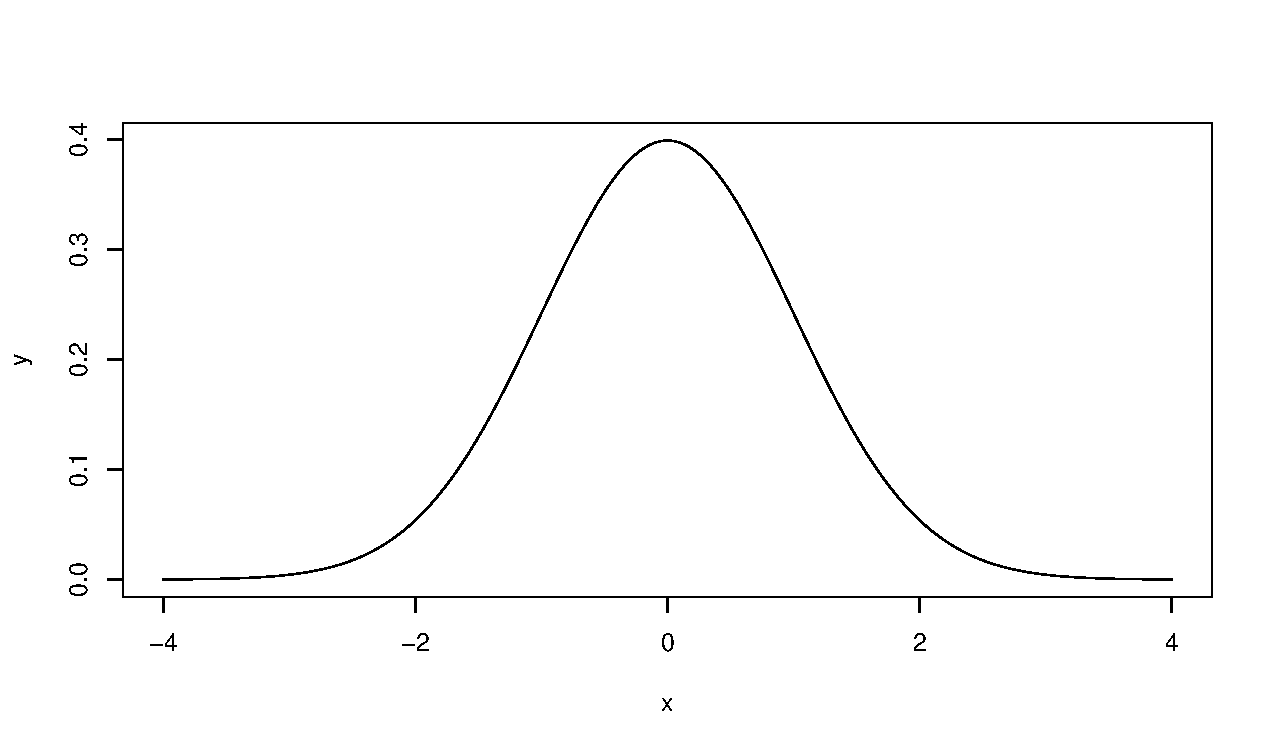
\includegraphics[width=\maxwidth]{figure/unnamed-chunk-32-1} 

}


\end{knitrout}

\code{type = "l"} is for a smooth line (instead of dots).

We can also plot $y=x^2$ for example.
\begin{knitrout}
\definecolor{shadecolor}{rgb}{0.969, 0.969, 0.969}\color{fgcolor}\begin{kframe}
\begin{alltt}
\hlstd{y} \hlkwb{<-} \hlstd{x} \hlopt{^} \hlnum{2}
\hlkwd{plot}\hlstd{(x, y,} \hlkwc{type} \hlstd{=} \hlstr{"l"}\hlstd{)}
\end{alltt}
\end{kframe}

{\centering 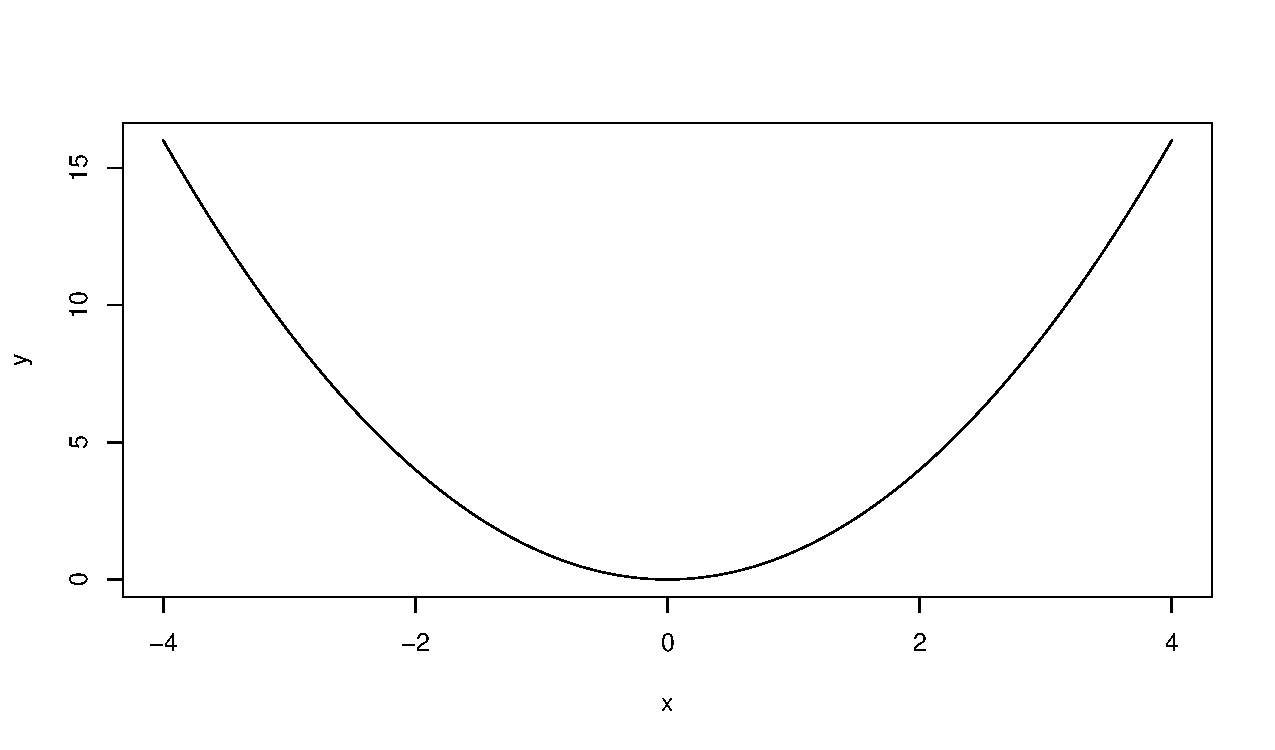
\includegraphics[width=\maxwidth]{figure/unnamed-chunk-33-1} 

}


\end{knitrout}

\subsubsection{F-distribution Examples}

\begin{knitrout}
\definecolor{shadecolor}{rgb}{0.969, 0.969, 0.969}\color{fgcolor}\begin{kframe}
\begin{alltt}
\hlstd{x} \hlkwb{<-} \hlkwd{seq}\hlstd{(}\hlnum{0}\hlstd{,}\hlnum{5}\hlstd{,}\hlnum{0.01}\hlstd{)}
\hlkwd{head}\hlstd{(x)}
\end{alltt}
\begin{verbatim}
## [1] 0.00 0.01 0.02 0.03 0.04 0.05
\end{verbatim}
\begin{alltt}
\hlcom{# df is degrees of freedom.}
\hlcom{# type = "l" is for a smooth curve}
\hlkwd{plot}\hlstd{(}
\hlstd{x,}
\hlkwc{y} \hlstd{=} \hlkwd{df}\hlstd{(x,} \hlkwc{df1} \hlstd{=} \hlnum{1}\hlstd{,} \hlkwc{df2} \hlstd{=} \hlnum{1}\hlstd{),}
\hlkwc{type} \hlstd{=} \hlstr{"l"}\hlstd{,}
\hlkwc{xlab} \hlstd{=} \hlstr{"x"}\hlstd{,}
\hlkwc{ylab} \hlstd{=} \hlstr{"density"}
\hlstd{)}
\end{alltt}
\end{kframe}

{\centering 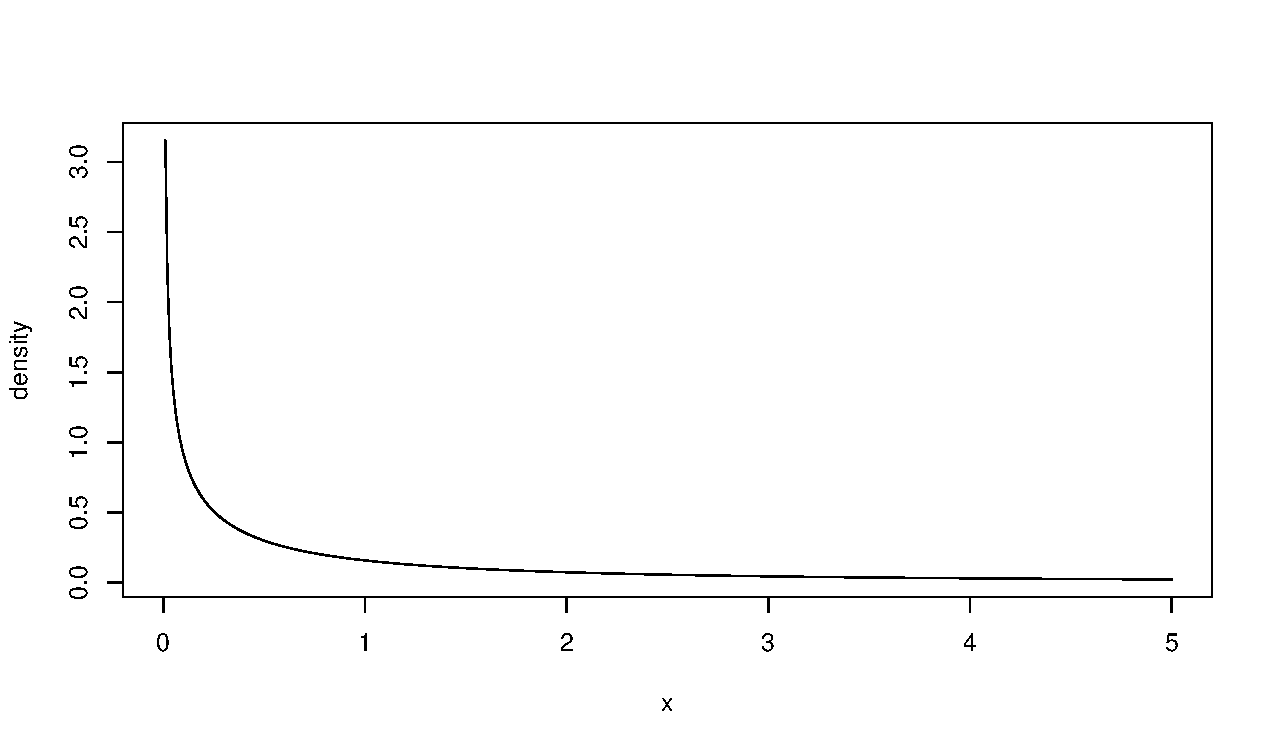
\includegraphics[width=\maxwidth]{figure/unnamed-chunk-34-1} 

}


\begin{kframe}\begin{alltt}
\hlcom{# ylim is for the y-axis limits}
\hlcom{# lwd is for line width}
\hlkwd{plot}\hlstd{(}
\hlstd{x,}
\hlkwc{y} \hlstd{=} \hlkwd{df}\hlstd{(x,} \hlkwc{df1} \hlstd{=} \hlnum{1}\hlstd{,} \hlkwc{df2} \hlstd{=} \hlnum{1}\hlstd{),}
\hlkwc{type} \hlstd{=} \hlstr{"l"}\hlstd{,}
\hlkwc{col} \hlstd{=} \hlstr{"black"}\hlstd{,}
\hlkwc{xlab} \hlstd{=} \hlstr{"x"}\hlstd{,}
\hlkwc{ylab} \hlstd{=} \hlstr{"density"}\hlstd{,}
\hlkwc{ylim} \hlstd{=} \hlkwd{c}\hlstd{(}\hlnum{0}\hlstd{,} \hlnum{2.5}\hlstd{),}
\hlkwc{lwd} \hlstd{=} \hlnum{2}
\hlstd{)}
\hlcom{# Add lines to the existing plot.}
\hlkwd{lines}\hlstd{(}
\hlstd{x,}
\hlkwc{y} \hlstd{=} \hlkwd{df}\hlstd{(x,} \hlkwc{df1} \hlstd{=} \hlnum{1}\hlstd{,} \hlkwc{df2} \hlstd{=} \hlnum{100}\hlstd{),}
\hlkwc{type} \hlstd{=} \hlstr{"l"}\hlstd{,}
\hlkwc{col} \hlstd{=} \hlstr{"green"}\hlstd{,}
\hlkwc{lwd} \hlstd{=} \hlnum{2}
\hlstd{)}
\hlkwd{lines}\hlstd{(}
\hlstd{x,}
\hlkwc{y} \hlstd{=} \hlkwd{df}\hlstd{(x,} \hlkwc{df1} \hlstd{=} \hlnum{5}\hlstd{,} \hlkwc{df2} \hlstd{=} \hlnum{1}\hlstd{),}
\hlkwc{type} \hlstd{=} \hlstr{"l"}\hlstd{,}
\hlkwc{col} \hlstd{=} \hlstr{"blue"}\hlstd{,}
\hlkwc{lwd} \hlstd{=} \hlnum{2}
\hlstd{)}
\hlkwd{lines}\hlstd{(}
\hlstd{x,}
\hlkwc{y} \hlstd{=} \hlkwd{df}\hlstd{(x,} \hlkwc{df1} \hlstd{=} \hlnum{5}\hlstd{,} \hlkwc{df2} \hlstd{=} \hlnum{100}\hlstd{),}
\hlkwc{type} \hlstd{=} \hlstr{"l"}\hlstd{,}
\hlkwc{col} \hlstd{=} \hlstr{"purple"}\hlstd{,}
\hlkwc{lwd} \hlstd{=} \hlnum{2}
\hlstd{)}
\hlkwd{lines}\hlstd{(}
\hlstd{x,}
\hlkwc{y} \hlstd{=} \hlkwd{df}\hlstd{(x,} \hlkwc{df1} \hlstd{=} \hlnum{10}\hlstd{,} \hlkwc{df2} \hlstd{=} \hlnum{1}\hlstd{),}
\hlkwc{type} \hlstd{=} \hlstr{"l"}\hlstd{,}
\hlkwc{col} \hlstd{=} \hlstr{"red"}\hlstd{,}
\hlkwc{lwd} \hlstd{=} \hlnum{2}
\hlstd{)}
\hlkwd{lines}\hlstd{(}
\hlstd{x,}
\hlkwc{y} \hlstd{=} \hlkwd{df}\hlstd{(x,} \hlkwc{df1} \hlstd{=} \hlnum{10}\hlstd{,} \hlkwc{df2} \hlstd{=} \hlnum{100}\hlstd{),}
\hlkwc{type} \hlstd{=} \hlstr{"l"}\hlstd{,}
\hlkwc{col} \hlstd{=} \hlstr{"orange"}\hlstd{,}
\hlkwc{lwd} \hlstd{=} \hlnum{2}
\hlstd{)}
\hlcom{# Add a legend to the top-right.}
\hlcom{# lty = 1 is for a straight solid line.}
\hlkwd{legend}\hlstd{(}
\hlstr{"topright"}\hlstd{,}
\hlkwc{legend} \hlstd{=} \hlkwd{c}\hlstd{(}
\hlstr{"df1=1, df2=1"}\hlstd{,}
\hlstr{"df1=1, df2=100"}\hlstd{,}
\hlstr{"df1=5, df2=1"}\hlstd{,}
\hlstr{"df1=5, df2=100"}\hlstd{,}
\hlstr{"df1=10, df2=1"}\hlstd{,}
\hlstr{"df1=10, df2=100"}
\hlstd{),}
\hlkwc{lty} \hlstd{=} \hlnum{1}\hlstd{,}
\hlkwc{col} \hlstd{=} \hlkwd{c}\hlstd{(}\hlstr{"black"}\hlstd{,} \hlstr{"green"}\hlstd{,} \hlstr{"blue"}\hlstd{,} \hlstr{"purple"}\hlstd{,} \hlstr{"red"}\hlstd{,} \hlstr{"orange"}\hlstd{)}
\hlstd{)}
\end{alltt}
\end{kframe}

{\centering 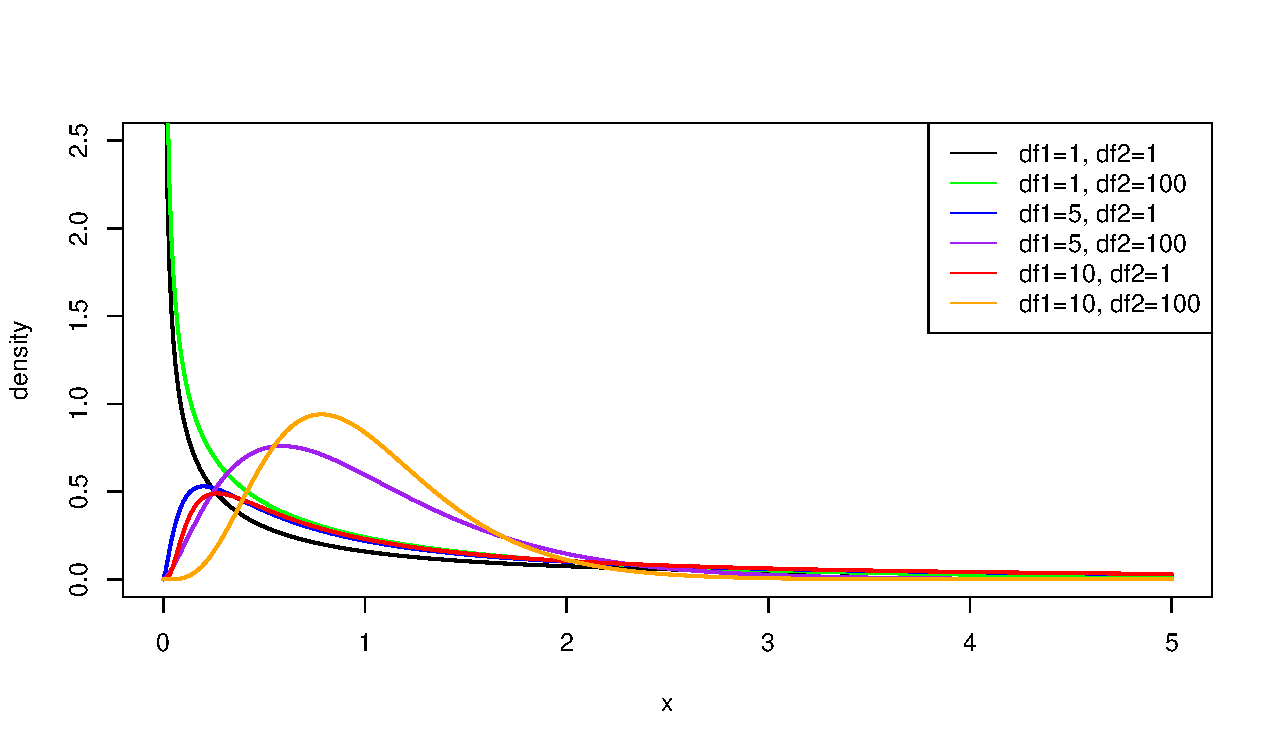
\includegraphics[width=\maxwidth]{figure/unnamed-chunk-34-2} 

}


\end{knitrout}

\subsubsection{Random numbers for the F-distribution}

\begin{knitrout}
\definecolor{shadecolor}{rgb}{0.969, 0.969, 0.969}\color{fgcolor}\begin{kframe}
\begin{alltt}
\hlcom{# set.seed allows for exact reproduction.}
\hlkwd{set.seed}\hlstd{(}\hlnum{12345678}\hlstd{)}
\hlstd{randF} \hlkwb{<-} \hlkwd{rf}\hlstd{(}\hlnum{1000}\hlstd{,} \hlnum{5}\hlstd{,} \hlnum{100}\hlstd{)}
\hlcom{# Generate histogram for the random numbers with exact.}
\hlkwd{hist}\hlstd{(randF)}
\end{alltt}
\end{kframe}

{\centering 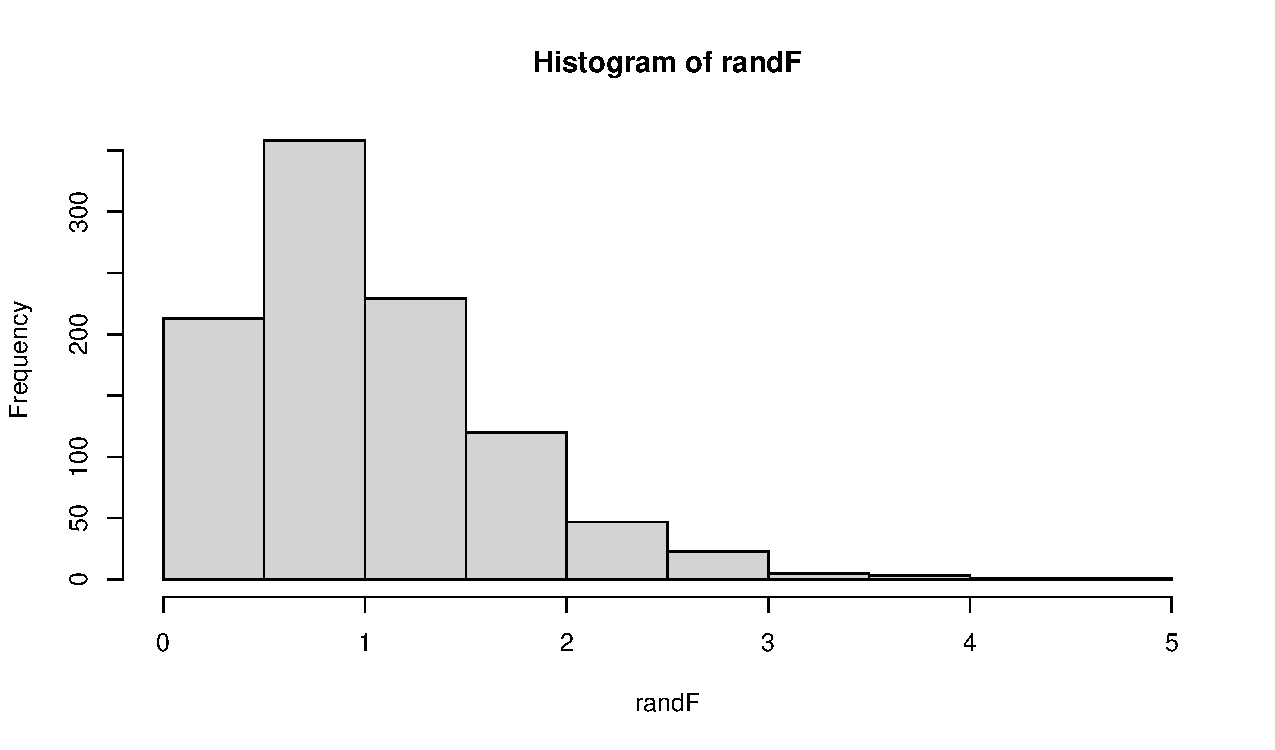
\includegraphics[width=\maxwidth]{figure/unnamed-chunk-35-1} 

}


\begin{kframe}\begin{alltt}
\hlcom{# Generate histogram for the random numbers with relative frequency.}
\hlcom{# This is normalized, so we can superimpose an F-distribution to it.}
\hlkwd{hist}\hlstd{(randF,} \hlkwc{freq} \hlstd{=} \hlnum{FALSE}\hlstd{)}
\hlcom{# Superimpose an F-distribution on the histogram.}
\hlkwd{lines}\hlstd{(}
\hlstd{x,}
\hlkwc{y} \hlstd{=} \hlkwd{df}\hlstd{(x,} \hlkwc{df1} \hlstd{=} \hlnum{5}\hlstd{,} \hlkwc{df2} \hlstd{=} \hlnum{100}\hlstd{),}
\hlkwc{type} \hlstd{=} \hlstr{"l"}\hlstd{,}
\hlkwc{col} \hlstd{=} \hlstr{"purple"}\hlstd{,}
\hlkwc{lwd} \hlstd{=} \hlnum{2}
\hlstd{)}
\end{alltt}
\end{kframe}

{\centering 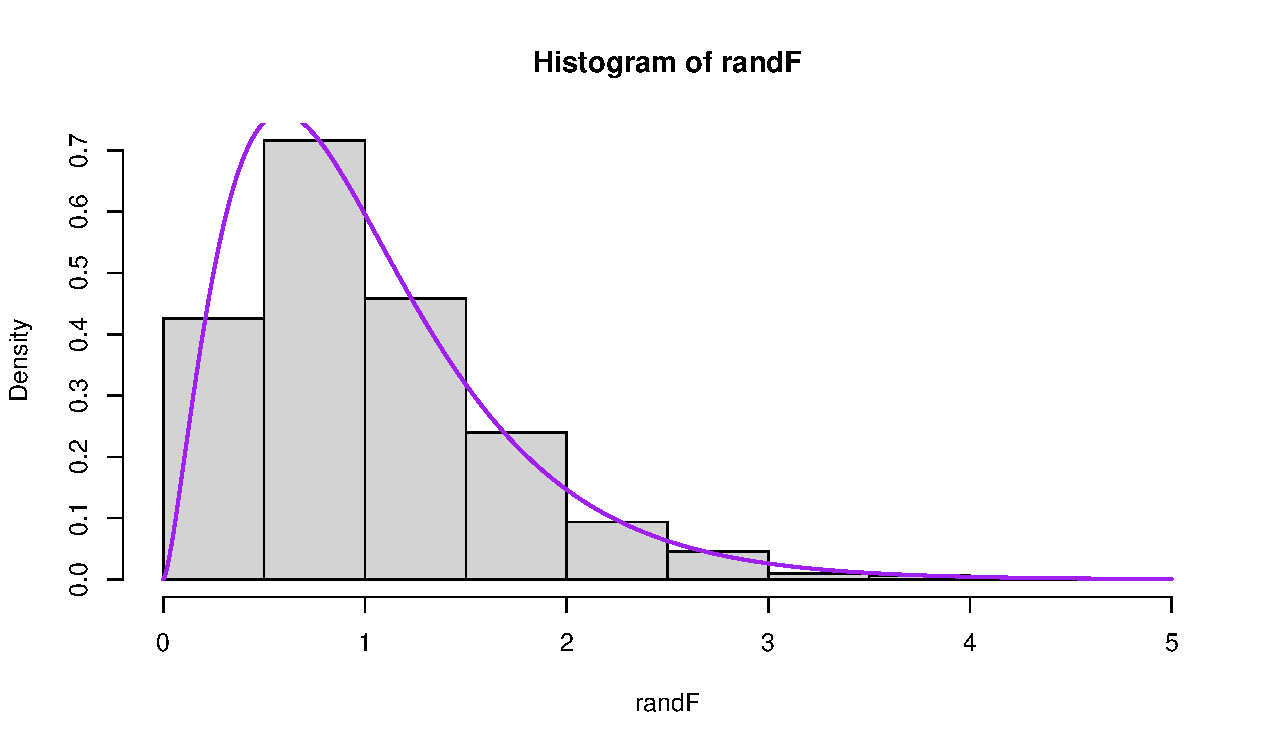
\includegraphics[width=\maxwidth]{figure/unnamed-chunk-35-2} 

}


\begin{kframe}\begin{alltt}
\hlcom{# Set y-axis limits and more detailed histogram bins using 'breaks = 25'}
\hlkwd{hist}\hlstd{(randF,}
\hlkwc{freq} \hlstd{=} \hlnum{FALSE}\hlstd{,}
\hlkwc{ylim} \hlstd{=} \hlkwd{c}\hlstd{(}\hlnum{0}\hlstd{,} \hlnum{0.8}\hlstd{),}
\hlkwc{breaks} \hlstd{=} \hlnum{25}\hlstd{)}
\hlkwd{lines}\hlstd{(}
\hlstd{x,}
\hlkwc{y} \hlstd{=} \hlkwd{df}\hlstd{(x,} \hlkwc{df1} \hlstd{=} \hlnum{5}\hlstd{,} \hlkwc{df2} \hlstd{=} \hlnum{100}\hlstd{),}
\hlkwc{type} \hlstd{=} \hlstr{"l"}\hlstd{,}
\hlkwc{col} \hlstd{=} \hlstr{"purple"}\hlstd{,}
\hlkwc{lwd} \hlstd{=} \hlnum{2}
\hlstd{)}
\end{alltt}
\end{kframe}

{\centering 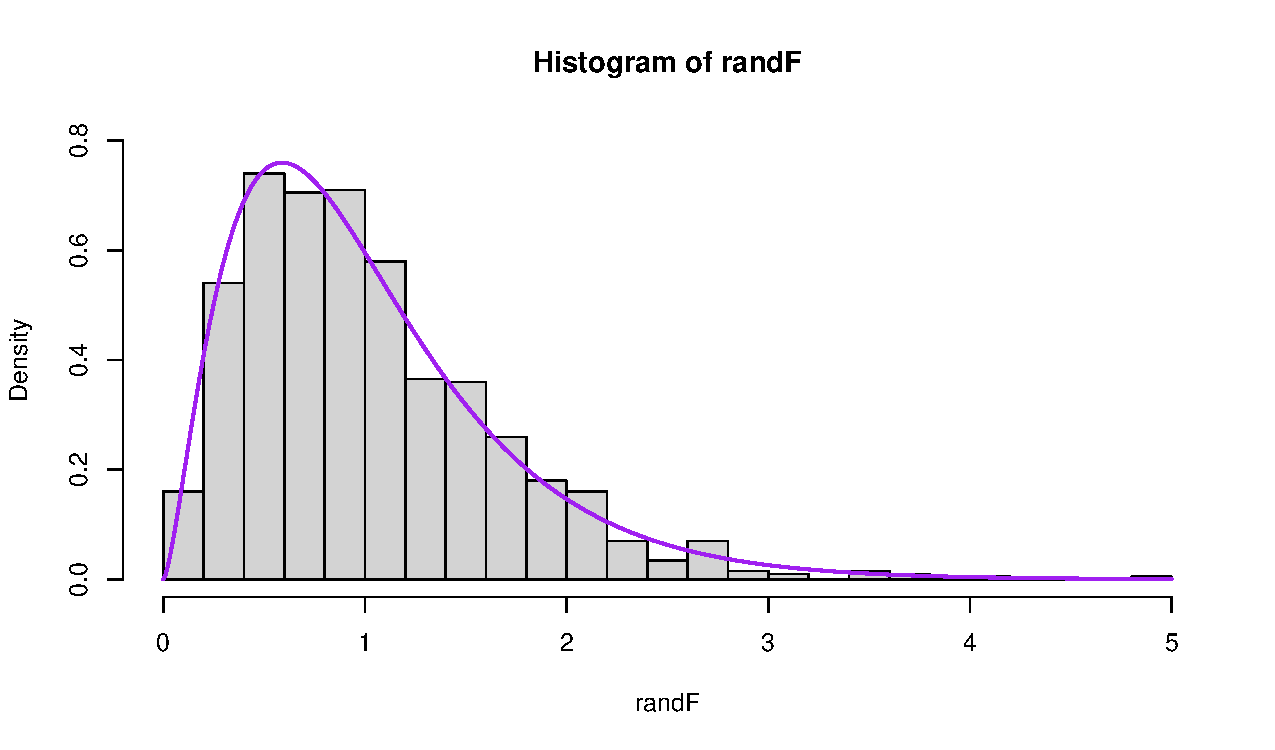
\includegraphics[width=\maxwidth]{figure/unnamed-chunk-35-3} 

}


\begin{kframe}\begin{alltt}
\hlcom{# Generate more random F-distributions to get closer to the 'true' density.}
\hlstd{randF} \hlkwb{<-} \hlkwd{rf}\hlstd{(}\hlnum{10000}\hlstd{,} \hlnum{5}\hlstd{,} \hlnum{100}\hlstd{)}
\hlkwd{hist}\hlstd{(randF,}
\hlkwc{freq} \hlstd{=} \hlnum{FALSE}\hlstd{,}
\hlkwc{ylim} \hlstd{=} \hlkwd{c}\hlstd{(}\hlnum{0}\hlstd{,} \hlnum{0.8}\hlstd{),}
\hlkwc{breaks} \hlstd{=} \hlnum{25}\hlstd{)}
\hlkwd{lines}\hlstd{(}
\hlstd{x,}
\hlkwc{y} \hlstd{=} \hlkwd{df}\hlstd{(x,} \hlkwc{df1} \hlstd{=} \hlnum{5}\hlstd{,} \hlkwc{df2} \hlstd{=} \hlnum{100}\hlstd{),}
\hlkwc{type} \hlstd{=} \hlstr{"l"}\hlstd{,}
\hlkwc{col} \hlstd{=} \hlstr{"purple"}\hlstd{,}
\hlkwc{lwd} \hlstd{=} \hlnum{2}
\hlstd{)}
\end{alltt}
\end{kframe}

{\centering 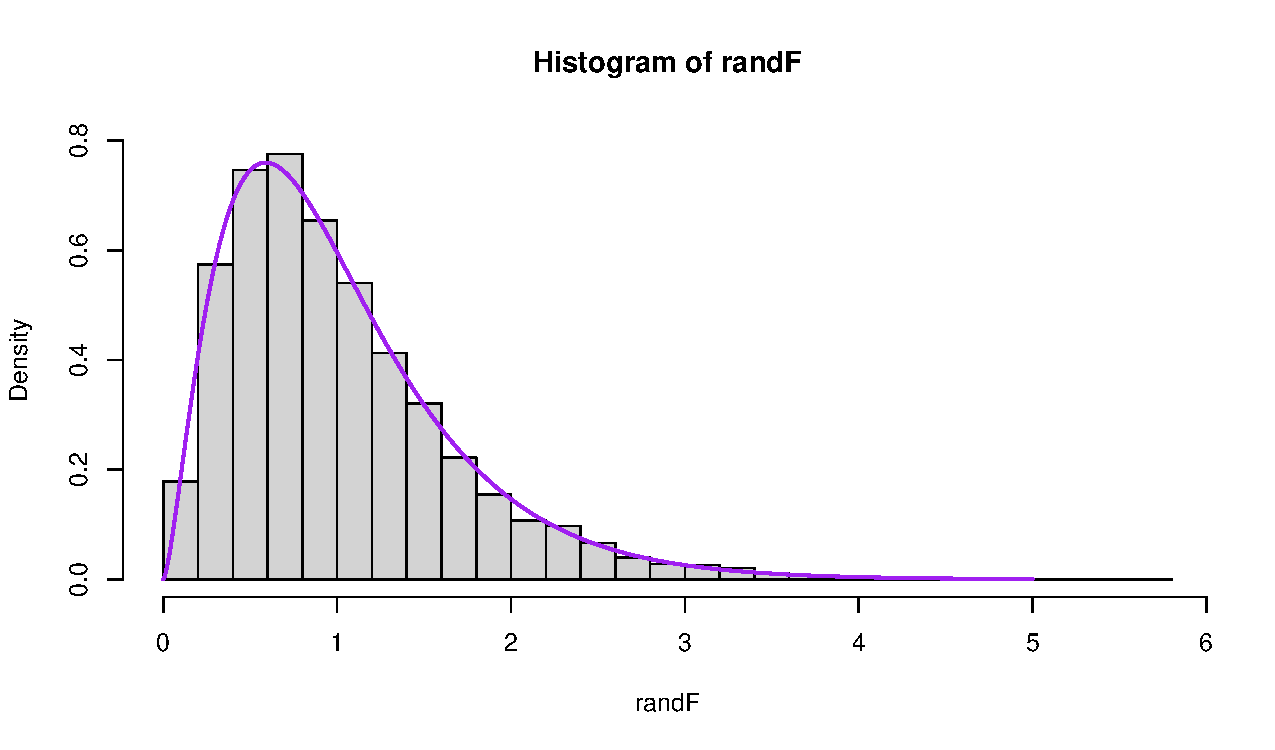
\includegraphics[width=\maxwidth]{figure/unnamed-chunk-35-4} 

}


\end{knitrout}

\subsubsection{Revisit Rocket Example}

\begin{knitrout}
\definecolor{shadecolor}{rgb}{0.969, 0.969, 0.969}\color{fgcolor}\begin{kframe}
\begin{alltt}
\hlstd{rocket} \hlkwb{<-} \hlkwd{read.csv}\hlstd{(}\hlstr{"csv/rocket.csv"}\hlstd{)}
\hlstd{m1} \hlkwb{<-} \hlkwd{lm}\hlstd{(thrust} \hlopt{~} \hlstd{nozzle} \hlopt{+} \hlstd{propratio,} \hlkwc{data} \hlstd{= rocket)}
\hlkwd{summary}\hlstd{(m1)}
\end{alltt}
\begin{verbatim}
## 
## Call:
## lm(formula = thrust ~ nozzle + propratio, data = rocket)
## 
## Residuals:
##     Min      1Q  Median      3Q     Max 
## -3.8459 -1.7555  0.5934  1.2906  3.3008 
## 
## Coefficients:
##             Estimate Std. Error t value Pr(>|t|)    
## (Intercept) 473.6039     4.7158 100.430 4.88e-15 ***
## nozzle       16.7383     1.5329  10.919 1.71e-06 ***
## propratio    -1.0948     0.9414  -1.163    0.275    
## ---
## Signif. codes:  0 '***' 0.001 '**' 0.01 '*' 0.05 '.' 0.1 ' ' 1
## 
## Residual standard error: 2.655 on 9 degrees of freedom
## Multiple R-squared:  0.9303,	Adjusted R-squared:  0.9148 
## F-statistic: 60.05 on 2 and 9 DF,  p-value: 6.238e-06
\end{verbatim}
\begin{alltt}
\hlcom{# Compare summary with ANOVA table on board from Oct. 5.}
\hlkwd{anova}\hlstd{(m1)}
\end{alltt}
\begin{verbatim}
## Analysis of Variance Table
## 
## Response: thrust
##           Df Sum Sq Mean Sq  F value    Pr(>F)    
## nozzle     1 836.67  836.67 118.7377 1.743e-06 ***
## propratio  1   9.53    9.53   1.3524    0.2748    
## Residuals  9  63.42    7.05                       
## ---
## Signif. codes:  0 '***' 0.001 '**' 0.01 '*' 0.05 '.' 0.1 ' ' 1
\end{verbatim}
\begin{alltt}
\hlkwd{anova}\hlstd{(m1)}\hlopt{$}\hlstd{`Sum Sq`}
\end{alltt}
\begin{verbatim}
## [1] 836.670000   9.529332  63.417335
\end{verbatim}
\begin{alltt}
    \hlkwd{sum}\hlstd{(}\hlkwd{anova}\hlstd{(m1)}\hlopt{$}\hlstd{`Sum Sq`[}\hlnum{1}\hlopt{:}\hlnum{2}\hlstd{])}
\end{alltt}
\begin{verbatim}
## [1] 846.1993
\end{verbatim}
\begin{alltt}
\hlstd{SSRes} \hlkwb{<-} \hlkwd{anova}\hlstd{(m1)}\hlopt{$}\hlstd{`Sum Sq`[}\hlnum{3}\hlstd{]}

    \hlcom{# Test of overall significance.}
    \hlstd{m_red} \hlkwb{<-} \hlkwd{lm}\hlstd{(thrust} \hlopt{~} \hlnum{1}\hlstd{,} \hlkwc{data} \hlstd{= rocket)}
    \hlkwd{summary}\hlstd{(m_red)}
\end{alltt}
\begin{verbatim}
## 
## Call:
## lm(formula = thrust ~ 1, data = rocket)
## 
## Residuals:
##      Min       1Q   Median       3Q      Max 
## -13.4167  -7.1167  -0.2167   8.2333  11.3833 
## 
## Coefficients:
##             Estimate Std. Error t value Pr(>|t|)    
## (Intercept)  476.617      2.625   181.6   <2e-16 ***
## ---
## Signif. codes:  0 '***' 0.001 '**' 0.01 '*' 0.05 '.' 0.1 ' ' 1
## 
## Residual standard error: 9.094 on 11 degrees of freedom
\end{verbatim}
\begin{alltt}
    \hlkwd{anova}\hlstd{(m_red)}
\end{alltt}
\begin{verbatim}
## Analysis of Variance Table
## 
## Response: thrust
##           Df Sum Sq Mean Sq F value Pr(>F)
## Residuals 11 909.62  82.692
\end{verbatim}
\begin{alltt}
    \hlstd{SSRes_A} \hlkwb{<-} \hlkwd{anova}\hlstd{(m_red)}\hlopt{$}\hlstd{`Sum Sq`[}\hlnum{1}\hlstd{]}

\hlcom{# Manually calculate F-statistic.}
\hlstd{l} \hlkwb{<-} \hlnum{2}
\hlstd{n} \hlkwb{<-} \hlkwd{nrow}\hlstd{(rocket)}
\hlstd{p} \hlkwb{<-} \hlnum{2}
\hlstd{Fstat} \hlkwb{<-} \hlstd{((SSRes_A} \hlopt{-} \hlstd{SSRes)} \hlopt{/} \hlstd{l)} \hlopt{/} \hlstd{(SSRes} \hlopt{/} \hlstd{(n} \hlopt{-} \hlstd{p} \hlopt{-} \hlnum{1}\hlstd{))}
\hlstd{Fstat}
\end{alltt}
\begin{verbatim}
## [1] 60.04505
\end{verbatim}
\begin{alltt}
\hlstd{pval} \hlkwb{<-} \hlnum{1} \hlopt{-} \hlkwd{pf}\hlstd{(Fstat,} \hlkwc{df1} \hlstd{= l,} \hlkwc{df2} \hlstd{= n} \hlopt{-} \hlstd{p} \hlopt{-} \hlnum{1}\hlstd{)}
\hlstd{pval}
\end{alltt}
\begin{verbatim}
## [1] 6.238398e-06
\end{verbatim}
\begin{alltt}
\hlcom{# Automatically calculate F-statistic.}
\hlkwd{anova}\hlstd{(m1, m_red)}\hlopt{$}\hlstd{F[}\hlnum{2}\hlstd{]}
\end{alltt}
\begin{verbatim}
## [1] 60.04505
\end{verbatim}
\end{kframe}
\end{knitrout}

    \subsubsection{Revist Coffee Example (Coffee Quality Institute, 2018)}

\begin{knitrout}
\definecolor{shadecolor}{rgb}{0.969, 0.969, 0.969}\color{fgcolor}\begin{kframe}
\begin{alltt}
\hlstd{coffee} \hlkwb{<-} \hlkwd{read.csv}\hlstd{(}\hlstr{"csv/coffee_arabica.csv"}\hlstd{)}

\hlstd{mfull} \hlkwb{<-}
\hlkwd{lm}\hlstd{(}
\hlstd{Flavor} \hlopt{~} \hlkwd{factor}\hlstd{(Processing.Method)} \hlopt{+} \hlstd{Aroma} \hlopt{+} \hlstd{Aftertaste} \hlopt{+}
\hlstd{Body} \hlopt{+} \hlstd{Acidity} \hlopt{+} \hlstd{Balance} \hlopt{+} \hlstd{Sweetness} \hlopt{+} \hlstd{Uniformity} \hlopt{+} \hlstd{Moisture,}
\hlkwc{dat} \hlstd{= coffee}
\hlstd{)}
\hlkwd{summary}\hlstd{(mfull)}
\end{alltt}
\begin{verbatim}
## 
## Call:
## lm(formula = Flavor ~ factor(Processing.Method) + Aroma + Aftertaste + 
##     Body + Acidity + Balance + Sweetness + Uniformity + Moisture, 
##     data = coffee)
## 
## Residuals:
##      Min       1Q   Median       3Q      Max 
## -0.68587 -0.08465  0.00079  0.08910  0.63633 
## 
## Coefficients:
##                                                     Estimate Std. Error t value
## (Intercept)                                        -0.728757   0.168516  -4.325
## factor(Processing.Method)Semi-washed / Semi-pulped -0.001396   0.022021  -0.063
## factor(Processing.Method)Washed / Wet              -0.033061   0.011024  -2.999
## Aroma                                               0.220302   0.020447  10.774
## Aftertaste                                          0.468759   0.023912  19.603
## Body                                                0.096140   0.024334   3.951
## Acidity                                             0.216751   0.021194  10.227
## Balance                                             0.046806   0.022558   2.075
## Sweetness                                           0.025507   0.010150   2.513
## Uniformity                                          0.016297   0.009803   1.663
## Moisture                                            0.169012   0.102480   1.649
##                                                    Pr(>|t|)    
## (Intercept)                                        1.67e-05 ***
## factor(Processing.Method)Semi-washed / Semi-pulped  0.94947    
## factor(Processing.Method)Washed / Wet               0.00277 ** 
## Aroma                                               < 2e-16 ***
## Aftertaste                                          < 2e-16 ***
## Body                                               8.28e-05 ***
## Acidity                                             < 2e-16 ***
## Balance                                             0.03823 *  
## Sweetness                                           0.01211 *  
## Uniformity                                          0.09669 .  
## Moisture                                            0.09938 .  
## ---
## Signif. codes:  0 '***' 0.001 '**' 0.01 '*' 0.05 '.' 0.1 ' ' 1
## 
## Residual standard error: 0.148 on 1108 degrees of freedom
## Multiple R-squared:  0.8091,	Adjusted R-squared:  0.8073 
## F-statistic: 469.5 on 10 and 1108 DF,  p-value: < 2.2e-16
\end{verbatim}
\begin{alltt}
\hlkwd{anova}\hlstd{(mfull)}
\end{alltt}
\begin{verbatim}
## Analysis of Variance Table
## 
## Response: Flavor
##                             Df Sum Sq Mean Sq   F value    Pr(>F)    
## factor(Processing.Method)    2  2.313   1.156   52.8096 < 2.2e-16 ***
## Aroma                        1 67.258  67.258 3071.2889 < 2.2e-16 ***
## Aftertaste                   1 29.097  29.097 1328.6722 < 2.2e-16 ***
## Body                         1  1.129   1.129   51.5460  1.28e-12 ***
## Acidity                      1  2.522   2.522  115.1618 < 2.2e-16 ***
## Balance                      1  0.116   0.116    5.2963 0.0215553 *  
## Sweetness                    1  0.251   0.251   11.4392 0.0007442 ***
## Uniformity                   1  0.064   0.064    2.9154 0.0880167 .  
## Moisture                     1  0.060   0.060    2.7200 0.0993839 .  
## Residuals                 1108 24.264   0.022                        
## ---
## Signif. codes:  0 '***' 0.001 '**' 0.01 '*' 0.05 '.' 0.1 ' ' 1
\end{verbatim}
\begin{alltt}
\hlstd{SSRes} \hlkwb{<-} \hlkwd{anova}\hlstd{(mfull)}\hlopt{$}\hlstd{`Sum Sq`[}\hlnum{10}\hlstd{]}

\hlcom{# Reduced model without Uniformity and Moisture (beta9=beta10=0):}
\hlstd{m_red} \hlkwb{<-}
\hlkwd{lm}\hlstd{(}
\hlstd{Flavor} \hlopt{~} \hlkwd{factor}\hlstd{(Processing.Method)} \hlopt{+} \hlstd{Aroma} \hlopt{+} \hlstd{Aftertaste} \hlopt{+}
\hlstd{Body} \hlopt{+} \hlstd{Acidity} \hlopt{+} \hlstd{Balance} \hlopt{+} \hlstd{Sweetness,}
\hlkwc{dat} \hlstd{= coffee}
\hlstd{)}
\hlkwd{summary}\hlstd{(m_red)}
\end{alltt}
\begin{verbatim}
## 
## Call:
## lm(formula = Flavor ~ factor(Processing.Method) + Aroma + Aftertaste + 
##     Body + Acidity + Balance + Sweetness, data = coffee)
## 
## Residuals:
##      Min       1Q   Median       3Q      Max 
## -0.67907 -0.08487  0.00054  0.08490  0.64763 
## 
## Coefficients:
##                                                     Estimate Std. Error t value
## (Intercept)                                        -0.606791   0.159741  -3.799
## factor(Processing.Method)Semi-washed / Semi-pulped  0.002275   0.021969   0.104
## factor(Processing.Method)Washed / Wet              -0.031115   0.011009  -2.826
## Aroma                                               0.221362   0.020472  10.813
## Aftertaste                                          0.470849   0.023858  19.735
## Body                                                0.087671   0.024102   3.637
## Acidity                                             0.219257   0.021182  10.351
## Balance                                             0.047526   0.022283   2.133
## Sweetness                                           0.032406   0.009597   3.377
##                                                    Pr(>|t|)    
## (Intercept)                                        0.000153 ***
## factor(Processing.Method)Semi-washed / Semi-pulped 0.917539    
## factor(Processing.Method)Washed / Wet              0.004795 ** 
## Aroma                                               < 2e-16 ***
## Aftertaste                                          < 2e-16 ***
## Body                                               0.000288 ***
## Acidity                                             < 2e-16 ***
## Balance                                            0.033160 *  
## Sweetness                                          0.000759 ***
## ---
## Signif. codes:  0 '***' 0.001 '**' 0.01 '*' 0.05 '.' 0.1 ' ' 1
## 
## Residual standard error: 0.1482 on 1110 degrees of freedom
## Multiple R-squared:  0.8081,	Adjusted R-squared:  0.8067 
## F-statistic: 584.2 on 8 and 1110 DF,  p-value: < 2.2e-16
\end{verbatim}
\begin{alltt}
\hlkwd{anova}\hlstd{(m_red)}
\end{alltt}
\begin{verbatim}
## Analysis of Variance Table
## 
## Response: Flavor
##                             Df Sum Sq Mean Sq  F value    Pr(>F)    
## factor(Processing.Method)    2  2.313   1.156   52.637 < 2.2e-16 ***
## Aroma                        1 67.258  67.258 3061.263 < 2.2e-16 ***
## Aftertaste                   1 29.097  29.097 1324.335 < 2.2e-16 ***
## Body                         1  1.129   1.129   51.378 1.387e-12 ***
## Acidity                      1  2.522   2.522  114.786 < 2.2e-16 ***
## Balance                      1  0.116   0.116    5.279 0.0217690 *  
## Sweetness                    1  0.251   0.251   11.402 0.0007591 ***
## Residuals                 1110 24.387   0.022                       
## ---
## Signif. codes:  0 '***' 0.001 '**' 0.01 '*' 0.05 '.' 0.1 ' ' 1
\end{verbatim}
\begin{alltt}
\hlstd{SSRes_A} \hlkwb{<-} \hlkwd{anova}\hlstd{(m_red)}\hlopt{$}\hlstd{`Sum Sq`[}\hlnum{8}\hlstd{]}

\hlcom{# Manually calculate F-statistic.}
\hlstd{l} \hlkwb{<-} \hlnum{2}
\hlstd{n} \hlkwb{<-} \hlkwd{nrow}\hlstd{(coffee)}
\hlstd{p} \hlkwb{<-} \hlnum{10}
\hlstd{Fstat} \hlkwb{<-} \hlstd{((SSRes_A} \hlopt{-} \hlstd{SSRes)} \hlopt{/} \hlstd{l)} \hlopt{/} \hlstd{(SSRes} \hlopt{/} \hlstd{(n} \hlopt{-} \hlstd{p} \hlopt{-} \hlnum{1}\hlstd{))}
\hlstd{Fstat}
\end{alltt}
\begin{verbatim}
## [1] 2.81769
\end{verbatim}
\begin{alltt}
\hlstd{pval} \hlkwb{<-} \hlnum{1} \hlopt{-} \hlkwd{pf}\hlstd{(Fstat,} \hlkwc{df1} \hlstd{= l,} \hlkwc{df2} \hlstd{= n} \hlopt{-} \hlstd{p} \hlopt{-} \hlnum{1}\hlstd{)}
\hlstd{pval}
\end{alltt}
\begin{verbatim}
## [1] 0.06017197
\end{verbatim}
\begin{alltt}
\hlcom{# Automatically calculate F-statistic.}
\hlkwd{anova}\hlstd{(mfull, m_red)}\hlopt{$}\hlstd{F[}\hlnum{2}\hlstd{]}
\end{alltt}
\begin{verbatim}
## [1] 2.81769
\end{verbatim}
\begin{alltt}
\hlcom{# Reduced model without Uniformity and Moisture and}
\hlcom{# setting effect of Dry = Semi (beta1=beta9=beta10=0)}
\hlcom{# 1 = wet, 0 otherwise}
\hlstd{coffee}\hlopt{$}\hlstd{method2} \hlkwb{<-} \hlkwd{ifelse}\hlstd{(coffee}\hlopt{$}\hlstd{Processing.Method} \hlopt
\hlkwd{c}\hlstd{(}\hlstr{'Natural / Dry'}\hlstd{,} \hlstr{'Semi-washed / Semi-pulped'}\hlstd{),}
\hlnum{0}\hlstd{,}
\hlnum{1}\hlstd{)}
\hlcom{# 1 = semi/dry, 0 o.w}
\hlstd{coffee}\hlopt{$}\hlstd{wet} \hlkwb{<-}
\hlkwd{ifelse}\hlstd{(coffee}\hlopt{$}\hlstd{Processing.Method} \hlopt{==} \hlstr{'Washed / Wet'}\hlstd{,} \hlnum{0}\hlstd{,} \hlnum{1}\hlstd{)}

\hlstd{m_red2} \hlkwb{<-} \hlkwd{lm}\hlstd{(Flavor} \hlopt{~} \hlstd{method2} \hlopt{+} \hlstd{Aroma} \hlopt{+} \hlstd{Aftertaste} \hlopt{+}
\hlstd{Body} \hlopt{+} \hlstd{Acidity} \hlopt{+} \hlstd{Balance} \hlopt{+} \hlstd{Sweetness,}
\hlkwc{dat} \hlstd{= coffee)}
\hlkwd{summary}\hlstd{(m_red2)}
\end{alltt}
\begin{verbatim}
## 
## Call:
## lm(formula = Flavor ~ method2 + Aroma + Aftertaste + Body + Acidity + 
##     Balance + Sweetness, data = coffee)
## 
## Residuals:
##      Min       1Q   Median       3Q      Max 
## -0.67906 -0.08508  0.00052  0.08490  0.64722 
## 
## Coefficients:
##              Estimate Std. Error t value Pr(>|t|)    
## (Intercept) -0.606597   0.159659  -3.799 0.000153 ***
## method2     -0.031543   0.010200  -3.092 0.002036 ** 
## Aroma        0.221408   0.020458  10.823  < 2e-16 ***
## Aftertaste   0.470861   0.023847  19.745  < 2e-16 ***
## Body         0.087561   0.024068   3.638 0.000287 ***
## Acidity      0.219266   0.021173  10.356  < 2e-16 ***
## Balance      0.047527   0.022273   2.134 0.033077 *  
## Sweetness    0.032462   0.009577   3.389 0.000725 ***
## ---
## Signif. codes:  0 '***' 0.001 '**' 0.01 '*' 0.05 '.' 0.1 ' ' 1
## 
## Residual standard error: 0.1482 on 1111 degrees of freedom
## Multiple R-squared:  0.8081,	Adjusted R-squared:  0.8069 
## F-statistic: 668.3 on 7 and 1111 DF,  p-value: < 2.2e-16
\end{verbatim}
\begin{alltt}
\hlkwd{anova}\hlstd{(m_red2)}
\end{alltt}
\begin{verbatim}
## Analysis of Variance Table
## 
## Response: Flavor
##              Df Sum Sq Mean Sq   F value    Pr(>F)    
## method2       1  2.313   2.313  105.3648 < 2.2e-16 ***
## Aroma         1 67.255  67.255 3063.8526 < 2.2e-16 ***
## Aftertaste    1 29.100  29.100 1325.6571 < 2.2e-16 ***
## Body          1  1.126   1.126   51.3088 1.434e-12 ***
## Acidity       1  2.522   2.522  114.9115 < 2.2e-16 ***
## Balance       1  0.116   0.116    5.2882 0.0216552 *  
## Sweetness     1  0.252   0.252   11.4883 0.0007249 ***
## Residuals  1111 24.388   0.022                        
## ---
## Signif. codes:  0 '***' 0.001 '**' 0.01 '*' 0.05 '.' 0.1 ' ' 1
\end{verbatim}
\begin{alltt}
\hlstd{SSRes_A} \hlkwb{<-} \hlkwd{anova}\hlstd{(m_red2)}\hlopt{$}\hlstd{`Sum Sq`[}\hlnum{8}\hlstd{]}

\hlcom{## Manually calculate F-statistic.}
\hlstd{l} \hlkwb{<-} \hlnum{3}
\hlstd{n} \hlkwb{<-} \hlkwd{nrow}\hlstd{(coffee)}
\hlstd{p} \hlkwb{<-} \hlnum{10}
\hlstd{Fstat} \hlkwb{<-} \hlstd{((SSRes_A} \hlopt{-} \hlstd{SSRes)} \hlopt{/} \hlstd{l)} \hlopt{/} \hlstd{(SSRes} \hlopt{/} \hlstd{(n} \hlopt{-} \hlstd{p} \hlopt{-} \hlnum{1}\hlstd{))}
\hlstd{Fstat}
\end{alltt}
\begin{verbatim}
## [1] 1.882046
\end{verbatim}
\begin{alltt}
\hlstd{pval} \hlkwb{<-} \hlnum{1} \hlopt{-} \hlkwd{pf}\hlstd{(Fstat,} \hlkwc{df1} \hlstd{= l,} \hlkwc{df2} \hlstd{= n} \hlopt{-} \hlstd{p} \hlopt{-} \hlnum{1}\hlstd{)}
\hlstd{pval}
\end{alltt}
\begin{verbatim}
## [1] 0.1308207
\end{verbatim}
\begin{alltt}
\hlcom{# Automatically calculate F-statistic.}
\hlkwd{anova}\hlstd{(mfull, m_red2)}\hlopt{$}\hlstd{F[}\hlnum{2}\hlstd{]}
\end{alltt}
\begin{verbatim}
## [1] 1.882046
\end{verbatim}
\end{kframe}
\end{knitrout}
\makeheading{Lecture 12 | 2020-10-18}
Today: introduce two commonly
used multivariate random variables.
\section{Multinomial Distribution}
\begin{Definition}{Multinomial distribution}{}
    $ (X_1,\ldots,X_k) $ are joint discrete
    random variables with joint p.f.\ given by
    \[ f(x_1,\ldots,x_k)=\Prob{X_1=x_1,\ldots,X_k=x_k}=
        \frac{n!}{x_1!x_2!\cdots x_k!}p_1^{x_1}\cdots p_k^{x_k} \]
    where $ x_i=0,1,\ldots,n $ ($ i=1,2,\ldots,k $). Furthermore,
    $ \sum_{i=1}^{k}x_i=n $, $ \sum_{i=1}^{k} p_i=1 $,
    for $ 0<p_i<1 $ $ i=1,\ldots,k $. Then,
    $ (X_1,\ldots,X_k) $ follows a \textbf{multinomial distribution}.
    \[ (X_1,\ldots,X_k)\sim \mult{n;p_1,\ldots,p_k} \]
\end{Definition}
\begin{Example}{Possible Application}{}
    \begin{itemize}
        \item there are $ k $ boxes and each box
              has same balls
        \item probability of choosing a ball from the
              $ i^{\text{th}} $ box is $ p_i $ for $ i=1,2,\ldots,k $.
        \item randomly choose $ n $ balls from $ k $ boxes.
    \end{itemize}
    Let $ X_i\coloneq $ number of boxes from the
    $ i^{\text{th}} $ box for $ i=1,2,\ldots,k $. Then,
    \[ (X_1,\ldots,X_k) \sim \mult{n;p_1,\ldots,p_k} \]
    Note: if there are only two boxes, then $ X_1\sim \bin{n,p_1} $.
\end{Example}
\begin{Proposition}{Properties --- Multinomial Distribution}{prop_multi}
    If $ (X_1,\ldots,X_k) \sim \mult{n;p_1,\ldots,p_k} $, then
    \begin{enumerate}[label=(\arabic*)]
        \item\label{prop_multi1} $ M(t_1,\ldots,t_k)=\E{e^{t_1 X_1+\cdots+t_k X_k}}=
                  (p_1e^{t_1}+\cdots+p_k e^{t_k})^n $
              where $ \abs{t_i}<\infty $ for $ i=1,\ldots,k $.
        \item\label{prop_multi2} $ X_i \sim \bin{n,p_i} $ for $ i=1,\ldots,k $.
        \item\label{prop_multi3} If $ T=X_i+X_j $ for $ i\neq j $, then
              $ T \sim \bin{n,p_i+p_j} $
        \item\label{prop_multi4} $ \Cov{X_i,X_j}=-n p_i p_j  $
              for $ i\neq j $
        \item\label{prop_multi5} The conditional probability
              function of $ X_i $ given $ X_j=x_j $ for $ i\neq j $ is
              \[ X_i\mid X_j=x_j \sim \bin*{n-x_j,
                      \frac{p_i}{1-p_j}} \]
        \item\label{prop_multi6} The conditional distribution of $ X_i $
              given $ T=X_i+X_j $ for $ i\neq j $ is
              \[ X_i\mid X_i+X_j \sim \bin*{t,\frac{p_i}{p_i+p_j} } \]
    \end{enumerate}
\end{Proposition}
\begin{Proof}{\ref{prop:prop_multi}}{}
    Proof of~\ref{prop_multi1}: Too long
    for my poor soul to type. Proof requires the Multinomial Theorem.

    Proof of~\ref{prop_multi2}: The moment
    generating function of $ X_i $ for $ i=1,\ldots,k $ is
    \[ M(0,\ldots,0,t,0,\ldots,0)=\left[ p_i e^{t_i}+(1-p_i) \right]^n
        \quad t_i\in\mathbb{R} \]
    which is the moment generating function of a
    $ \bin{n,p_i} $ random variable. By~\ref{thm:uniq_mgf}
    we have $ X_i \sim \bin{n,p_i} $ for $ i=1,\ldots,k $.

    Proof of~\ref{prop_multi3}: The moment
    generating function of $ T=X_i+X_j $ for $ i\neq j $ is
    \begin{align*}
        M_T(t)
         & =\E*{e^{tT}}                                                                         \\
         & =\E*{e^{t(X_i+X_j)}}                                                                 \\
         & =\E*{e^{t X_i+t X_j}}                                                                \\
         & =M(0,\ldots,0,t,0,\ldots,0,t,0,\ldots,0)                                             \\
         & =(p_1+\cdots+p_i e^{t}+\cdots+p_j e^t+\cdots+p_{k-1}+p_k)^n & \quad & t\in\mathbb{R} \\
         & =\left[ (p_i+p_j)e^t+(1-p_i-p_j) \right]^n                  &       & t\in\mathbb{R}
    \end{align*}
    which is the moment generating function of a
    $ \bin{n,p_i+p_j} $ random variable. By~\ref{thm:uniq_mgf}
    we have $ T \sim \bin{n,p_i+p_j} $ for $ i\neq j $.

    Proof of~\ref{prop_multi4}:
    By~\ref{prop_multi2} we have $ \E{X_i}=n p_i $, $ \Var{X_i}=np_i(1-p_i) $,
    and $ \Var{X_j}=np_j(1-p_j) $. By~\ref{prop_multi3} we have
    $ X_i+X_j \sim \bin{n,p_i+p_j} $, so
    $ \Var{X_i+X_j}=n(p_i+p_j)(1-p_i-p_j) $.
    Thus,
    \[ \Cov{X_i+X_j,X_i+X_j}=\Var{X_i}+\Var{X_j}+2\Cov{X_i,X_j} \]
    \[ \implies n(p_i+p_j)(1-p_i-p_j)=np_i(1-p_i)+np_j(1-p_j)
        +2\Cov{X_i,X_j} \]
    Therefore, $ \Cov{X_i,X_j}=-n p_i p_j $.

    Proof of~\ref{prop_multi5}: There are $ x_j $ outcomes
    from the $ j^{\text{th}} $ category. Therefore,
    there are $ (n-x_j) $ balls chosen from the remaining $ (k-1) $
    boxes. We are not allowed to choose from the $ j^{\text{th}} $ box,
    we are only allowed to choose from the remaining $ (k-1) $
    boxes. Therefore, proportionally we get the success probability
    as $ p_i/(1-p_j) $.
\end{Proof}
\begin{Exercise}{}{}
    Prove property~\ref{prop_multi6} from~\Cref{prop:prop_multi}.
\end{Exercise}
\section{Bivariate Normal Distribution}
\begin{Definition}{Bivariate normal distribution}{}
    Suppose that $ X_1 $ and $ X_2 $
    are continuous random variables with joint probability
    density function
    \[ f(x_1,x_2)=\frac{1}{2\pi\abs*{\Sigma}^{1/2}}
        \exp\left\{ -\frac{1}{2}(\symbf{x}-\symbf{\mu})^\top \Sigma^{-1}(\symbf{x}-\symbf{\mu})
        \right\}\quad(x_1,x_2)\in\mathbb{R}^2     \]
    Also,
    \[ \symbf{x}=\begin{bmatrix}
            x_1 \\
            x_2
        \end{bmatrix}_{2\times 1},\quad
        \symbf{\mu}=\begin{bmatrix}
            \mu_1 \\
            \mu_2
        \end{bmatrix}_{2\times 1},\quad
        \Sigma=
        \begin{bmatrix}
            \sigma_1^2        & p\sigma_1\sigma_2 \\
            p\sigma_1\sigma_2 & \sigma_2^2
        \end{bmatrix}_{k\times k} \]
    and $ \Sigma $ is positive semi-definite. Also,
    $ \abs*{\Sigma} $ is the determinant of $ \Sigma $.
    Then, $ \symbf{X}=(X_1,X_2) $ follows a \textbf{bivariate normal distribution},
    and we write
    \[ \symbf{X}\sim\Bvn{\symbf{\mu},\Sigma}  \]
\end{Definition}
\begin{Remark}{$ \dagger $}{}
    Alternatively, we could write
    \begin{align*}
        f(x_1 & ,x_2)                                          \\
              & =\frac{1}{2\pi\sigma_1\sigma_2\sqrt{1-\rho^2}}
        \exp\left\{ -\frac{1}{2(1-\rho^2)}
        \left[ \left( \frac{x_1-\mu_1}{\sigma_1}  \right)^2+
            \left( \frac{x_2-\mu_2}{\sigma_2}  \right)^2-
            \frac{2\rho(x_1-\mu_1)(x_2-\mu_2)}{\sigma_1\sigma_2} \right] \right\}
    \end{align*}
\end{Remark}
\begin{Proposition}{Properties --- Bivariate Normal Distribution}{}
    \begin{enumerate}[label=(\arabic*)]
        \item $ X_1,X_2 $ has joint moment generating function
              \[ M(t_1,t_2)=\E{
                      e^{t_1X_1+t_2X_2}
                  }=\exp\left\{ \symbf{t}^\top \symbf{\mu}+\frac{1}{2}\symbf{t}^\top \Sigma
                  \symbf{t} \right\}\quad \forall t\in\mathbb{R}^2 \]
        \item Marginally,
              \[ M_{X_1}(t_1)=M(t_1,0)=\exp\left\{ t_1\mu_1+\frac{1}{2} t_1^2
                  \sigma_1^2\right\} \]
              which is the m.g.f.\ of $ N(\mu_1,\sigma_1^2) $; that is,
              $ X_1 \sim N(\mu_1,\sigma_1^2) $. Also,
              $ \E{X_1}=\mu_1 $ and $ \Var{X_1}=\sigma_1^2 $.
              \[ M_{X_2}(t_2)=M(0,t_2)=\exp\left\{ t_2\mu_2+\frac{1}{2} t_2^2
                  \sigma_2^2\right\} \]
              which is the m.g.f.\ of $ N(\mu_2,\sigma_2^2) $; that is,
              $ X_2 \sim N(\mu_2,\sigma_2^2) $. Also,
              $ \E{X_2}=\mu_2 $ and $ \Var{X_2}=\sigma_2^2 $.
        \item Conditional distribution.
              \[ X_2\mid X_1=x_1 \sim N
                  \left( \mu_2+\frac{\rho\sigma_2(x_1-\mu_1)}{\sigma_1} ,
                  \sigma_2^2(1-\rho^2) \right) \]
              \[ X_1\mid X_2=x_2 \sim N
                  \left( \mu_1+\frac{\rho\sigma_1(x_2-\mu_2)}{\sigma_2} ,
                  \sigma_1^2(1-\rho^2) \right) \]
              \[ f_2(x_2\mid x_1)=\frac{f(x_1,x_2)}{f_1(x_1)}  \]
              \[ f_1(x_1\mid x_2)=\frac{f(x_1,x_2)}{f_2(x_2)}  \]
        \item $ \Cov{X_1,X_2}=\rho\sigma_1\sigma_2 $
        \item $ \rho=0\iff X_1\text{ and }X_2 $ are independent.
        \item Linear transformations of bivariate
              normal are still normal.
        \item $ (\symbf{X}-\symbf{\mu})^\top \Sigma^{-1}(\symbf{X}-\symbf{\mu})\sim \chi^2(2) $
    \end{enumerate}
\end{Proposition}

4. \[ \E{X_1X_2}=\E{\E{X_1X_2\given X_1}} \]
Step 1: $ \E{X_1X_2\given X_1=x_1}=\E{x_1X_2\given X_1=x_1}=
    x_1\E{X_2\given X_1=x_1}=x_1
    \left(  \mu_2+\frac{\rho\sigma_2(x_1-\mu_1)}{\sigma_1} \right) $

Step 2:
\[ \E{X_1X_2\given X_1}=X_1
    \left(  \mu_2+\frac{\rho\sigma_2(X_1-\mu_1)}{\sigma_1} \right)
\]
\begin{align*}
    \E{X_1X_2}
     & = \E*{X_1\mu_2+\frac{X_1\rho\sigma_2(X_1-\mu_1)}{\sigma_1}}                         \\
     & =\mu_2\E{X_1}+\frac{\rho\sigma_2}{\sigma_1}
    \left[ \E{X_1^2}-\mu_1\E{X_1} \right]                                                  \\
     & =\mu_2\mu_1+\frac{\rho\sigma_2}{\sigma_1} \left[ \mu_1^2+\sigma_1^2-\mu_1^2 \right] \\
     & =\mu_1\mu_2+\rho\sigma_1\sigma_2
\end{align*}
Thus,
\[ \Cov{X_1,X_2}=\E{X_1X_2}-\frac{\E{X_1}\E{X_2}}{\mu_1\mu_2}=\rho\sigma_1\sigma_2  \]
\[ \Corr{X_1,X_2}=\frac{\Cov{X_1,X_2}}{\sqrt{\Var{X_1}\Var{X_2}}}=\rho  \]

5. We know if $ X_1 $ and $ X_2 $ are independent, then $ \rho=0 $.
If $ \rho=0 $, e.g. $ X_2\given X_1=x_1 \sim N(\mu_2,\sigma_1^2) $
and $ X_1\given X_2=x_2 \sim N(\mu_1,\sigma_1^2) $
In summary: If joint bivariate normal then uncorrelated = independence.

6. Let $ \symbf{c}=\begin{pmatrix}
        c_1 \\
        c_2
    \end{pmatrix} $, then
$ \symbf{c}^\top X=c_1X_2+c_2X_2 \sim N $ with
\[ \E{\symbf{c}^\top X}=c_1\mu_1+c_2\mu_2 \]
\[ \Var{\symbf{c}^\top X}=\symbf{c}^\top \Sigma\symbf{c} \]
Furthermore, $ A\in\mathbb{R}^{2\times 2} $,
$ \symbf{b}=\begin{pmatrix}
        b_1 \\
        b_2
    \end{pmatrix} $
\[ AX+\symbf{b} \sim \Bvn{A\symbf{\mu}+\symbf{b},A\Sigma A^\top} \]
Two linear combinations of BVN is joint BVN.\

7. Note $ \chi^2(1)\coloneq Z^2 $ where $ Z \sim \N{0,1} $.
\[ \chi^2(n)=
    \sum_{i=1}^{n} Z_i^2 \]
where $ Z_1,\ldots,Z_n $ are independent $ \N{0,1} $.


\subsection{R Demo}
\begin{knitrout}
\definecolor{shadecolor}{rgb}{0.969, 0.969, 0.969}\color{fgcolor}\begin{kframe}
\begin{alltt}
\hlcom{## Coffee example (Coffee Quality Institute, 2018) continued}
\hlstd{coffee} \hlkwb{<-} \hlkwd{read.csv}\hlstd{(}\hlstr{"csv/coffee_arabica.csv"}\hlstd{)}

\hlcom{# cor(coffee) doesn't work as there's a categorical variable.}
\hlkwd{cor}\hlstd{(coffee[,} \hlopt{-}\hlnum{1}\hlstd{])} \hlcom{# e.g., remove first column}
\end{alltt}
\begin{verbatim}
##                  Aroma     Flavor Aftertaste        Body     Acidity    Balance
## Aroma       1.00000000  0.7339782  0.6892744  0.56699932  0.60115765  0.6156508
## Flavor      0.73397820  1.0000000  0.8582783  0.67694834  0.73845546  0.7324530
## Aftertaste  0.68927440  0.8582783  1.0000000  0.67407704  0.69408861  0.7657979
## Body        0.56699932  0.6769483  0.6740770  1.00000000  0.60795391  0.6924568
## Acidity     0.60115765  0.7384555  0.6940886  0.60795391  1.00000000  0.6417994
## Balance     0.61565084  0.7324530  0.7657979  0.69245676  0.64179938  1.0000000
## Sweetness   0.06955938  0.1345364  0.1185760  0.03977892  0.06906093  0.1016718
## Uniformity  0.14785498  0.2132347  0.2143116  0.07195778  0.14876428  0.2180726
## Moisture   -0.11567549 -0.1327342 -0.1745366 -0.21009097 -0.10391684 -0.2161964
##             Sweetness Uniformity    Moisture
## Aroma      0.06955938 0.14785498 -0.11567549
## Flavor     0.13453644 0.21323472 -0.13273418
## Aftertaste 0.11857600 0.21431157 -0.17453658
## Body       0.03977892 0.07195778 -0.21009097
## Acidity    0.06906093 0.14876428 -0.10391684
## Balance    0.10167183 0.21807265 -0.21619640
## Sweetness  1.00000000 0.34756414  0.08049300
## Uniformity 0.34756414 1.00000000  0.02105693
## Moisture   0.08049300 0.02105693  1.00000000
\end{verbatim}
\end{kframe}
\end{knitrout}

Plot the pairs (disabled due to loading time on PDF).

\begin{knitrout}
\definecolor{shadecolor}{rgb}{0.969, 0.969, 0.969}\color{fgcolor}\begin{kframe}
\begin{alltt}
\hlkwd{pairs}\hlstd{(}
\hlopt{~} \hlstd{Flavor} \hlopt{+} \hlstd{Aroma} \hlopt{+} \hlstd{Aftertaste} \hlopt{+} \hlstd{Body} \hlopt{+}
\hlstd{Acidity} \hlopt{+} \hlstd{Balance} \hlopt{+} \hlstd{Sweetness} \hlopt{+} \hlstd{Uniformity} \hlopt{+} \hlstd{Moisture,}
\hlkwc{data} \hlstd{= coffee}
\hlstd{)}
\end{alltt}
\end{kframe}
\end{knitrout}

\begin{knitrout}
\definecolor{shadecolor}{rgb}{0.969, 0.969, 0.969}\color{fgcolor}\begin{kframe}
\begin{alltt}
\hlcom{# Code our own indicators, so that we can more easily interpret VIFs.}
\hlcom{# 1 = wet, 0 otherwise}
\hlstd{coffee}\hlopt{$}\hlstd{wet} \hlkwb{<-}
    \hlkwd{ifelse}\hlstd{(coffee}\hlopt{$}\hlstd{Processing.Method} \hlopt{==} \hlstr{'Washed / Wet'}\hlstd{,} \hlnum{1}\hlstd{,} \hlnum{0}\hlstd{)}
\hlcom{# 1 = semi/dry, 0 otherwise}
\hlstd{coffee}\hlopt{$}\hlstd{semi} \hlkwb{<-}
    \hlkwd{ifelse}\hlstd{(coffee}\hlopt{$}\hlstd{Processing.Method} \hlopt{==} \hlstr{'Semi-washed / Semi-pulped'}\hlstd{,}
\hlnum{1}\hlstd{,} \hlnum{0}\hlstd{)}
\end{alltt}
\end{kframe}
\end{knitrout}

Model:
$$y_i=\beta_0+\beta_1x_{i1}+\beta_2x_{i2}+\beta_3x_{i3}+
    \beta_4x_{i4}+\beta_5x_{i5}+\beta_6x_{i6}+\beta_7x_{i7}+\beta_8x_{i8}+
    \beta_9x_{i9}+\beta_{10}x_{i(10)}+\varepsilon_i$$
where
\begin{itemize}
    \item $y=$ flavour
    \item $x_1=1$ if wet, 0 otherwise
    \item $x_2=1$ if semi, 0 otherwise
    \item $x_3=$ Aroma
    \item $x_4=$ Aftertaste
    \item $x_5=$ Body
    \item $x_6=$ Acidity
    \item $x_7=$ Balance
    \item $x_8=$ Sweetness
    \item $x_9=$ Uniformity
    \item $x_{10}=$ Moisture
\end{itemize}

\begin{knitrout}
\definecolor{shadecolor}{rgb}{0.969, 0.969, 0.969}\color{fgcolor}\begin{kframe}
\begin{alltt}
\hlcom{# Full MLR with our manually coded indicators.}
\hlstd{mfull} \hlkwb{<-} \hlkwd{lm}\hlstd{(}
\hlstd{Flavor} \hlopt{~} \hlstd{wet} \hlopt{+} \hlstd{semi} \hlopt{+} \hlstd{Aroma} \hlopt{+} \hlstd{Aftertaste} \hlopt{+}
\hlstd{Body} \hlopt{+} \hlstd{Acidity} \hlopt{+} \hlstd{Balance} \hlopt{+} \hlstd{Sweetness} \hlopt{+} \hlstd{Uniformity} \hlopt{+} \hlstd{Moisture,}
\hlkwc{dat} \hlstd{= coffee}
\hlstd{)}
\hlkwd{summary}\hlstd{(mfull)}
\end{alltt}
\begin{verbatim}
## 
## Call:
## lm(formula = Flavor ~ wet + semi + Aroma + Aftertaste + Body + 
##     Acidity + Balance + Sweetness + Uniformity + Moisture, data = coffee)
## 
## Residuals:
##      Min       1Q   Median       3Q      Max 
## -0.68587 -0.08465  0.00079  0.08910  0.63633 
## 
## Coefficients:
##              Estimate Std. Error t value Pr(>|t|)    
## (Intercept) -0.728757   0.168516  -4.325 1.67e-05 ***
## wet         -0.033061   0.011024  -2.999  0.00277 ** 
## semi        -0.001396   0.022021  -0.063  0.94947    
## Aroma        0.220302   0.020447  10.774  < 2e-16 ***
## Aftertaste   0.468759   0.023912  19.603  < 2e-16 ***
## Body         0.096140   0.024334   3.951 8.28e-05 ***
## Acidity      0.216751   0.021194  10.227  < 2e-16 ***
## Balance      0.046806   0.022558   2.075  0.03823 *  
## Sweetness    0.025507   0.010150   2.513  0.01211 *  
## Uniformity   0.016297   0.009803   1.663  0.09669 .  
## Moisture     0.169012   0.102480   1.649  0.09938 .  
## ---
## Signif. codes:  0 '***' 0.001 '**' 0.01 '*' 0.05 '.' 0.1 ' ' 1
## 
## Residual standard error: 0.148 on 1108 degrees of freedom
## Multiple R-squared:  0.8091,	Adjusted R-squared:  0.8073 
## F-statistic: 469.5 on 10 and 1108 DF,  p-value: < 2.2e-16
\end{verbatim}
\begin{alltt}
\hlcom{# Full MLR alternative, using the factor command.}
\hlstd{mfull_alternative} \hlkwb{<-}
\hlkwd{lm}\hlstd{(}
\hlstd{Flavor} \hlopt{~} \hlkwd{factor}\hlstd{(Processing.Method)} \hlopt{+} \hlstd{Aroma} \hlopt{+} \hlstd{Aftertaste} \hlopt{+}
\hlstd{Body} \hlopt{+} \hlstd{Acidity} \hlopt{+} \hlstd{Balance} \hlopt{+} \hlstd{Sweetness} \hlopt{+} \hlstd{Uniformity} \hlopt{+} \hlstd{Moisture,}
\hlkwc{dat} \hlstd{= coffee}
\hlstd{)}
\end{alltt}
\end{kframe}
\end{knitrout}

Suppose we want to check the VIF for $j=1$; that is,
$x_1$. Now, we fit:
$$x_{i1}=\alpha_0+\alpha_2x_{i2}+\alpha_3x_{i3}+
    \alpha_4x_{i4}+\alpha_5x_{i5}+\alpha_6x_{i6}+\alpha_7x_{i7}+\alpha_8x_{i8}+
    \alpha_9x_{i9}+\alpha_{10}x_{i(10)}+\varepsilon_i$$

\begin{knitrout}
\definecolor{shadecolor}{rgb}{0.969, 0.969, 0.969}\color{fgcolor}\begin{kframe}
\begin{alltt}
\hlstd{wet_reg} \hlkwb{<-}
\hlkwd{lm}\hlstd{(}
\hlstd{wet} \hlopt{~} \hlstd{semi} \hlopt{+} \hlstd{Aroma} \hlopt{+} \hlstd{Aftertaste} \hlopt{+} \hlstd{Body} \hlopt{+} \hlstd{Acidity} \hlopt{+} \hlstd{Balance} \hlopt{+}
\hlstd{Sweetness} \hlopt{+} \hlstd{Uniformity} \hlopt{+} \hlstd{Moisture,}
\hlkwc{dat} \hlstd{= coffee}
\hlstd{)}
\hlkwd{summary}\hlstd{(wet_reg)}
\end{alltt}
\begin{verbatim}
## 
## Call:
## lm(formula = wet ~ semi + Aroma + Aftertaste + Body + Acidity + 
##     Balance + Sweetness + Uniformity + Moisture, data = coffee)
## 
## Residuals:
##     Min      1Q  Median      3Q     Max 
## -1.0015 -0.0283  0.1770  0.2522  0.7704 
## 
## Coefficients:
##             Estimate Std. Error t value Pr(>|t|)    
## (Intercept)  0.81748    0.45838   1.783 0.074794 .  
## semi        -0.75675    0.05551 -13.632  < 2e-16 ***
## Aroma        0.09690    0.05562   1.742 0.081774 .  
## Aftertaste  -0.13169    0.06502  -2.026 0.043054 *  
## Body        -0.21885    0.06596  -3.318 0.000936 ***
## Acidity      0.18696    0.05746   3.254 0.001173 ** 
## Balance     -0.10804    0.06136  -1.761 0.078563 .  
## Sweetness    0.08373    0.02753   3.041 0.002413 ** 
## Uniformity   0.03547    0.02668   1.329 0.184053    
## Moisture     0.59486    0.27858   2.135 0.032956 *  
## ---
## Signif. codes:  0 '***' 0.001 '**' 0.01 '*' 0.05 '.' 0.1 ' ' 1
## 
## Residual standard error: 0.4031 on 1109 degrees of freedom
## Multiple R-squared:  0.1911,	Adjusted R-squared:  0.1845 
## F-statistic: 29.11 on 9 and 1109 DF,  p-value: < 2.2e-16
\end{verbatim}
\begin{alltt}
\hlstd{r2_wet} \hlkwb{<-} \hlkwd{summary}\hlstd{(wet_reg)}\hlopt{$}\hlstd{r.squared}
    \hlstd{r2_wet}
\end{alltt}
\begin{verbatim}
## [1] 0.191077
\end{verbatim}
\end{kframe}
\end{knitrout}

$R_j$: In our case, $R_1=0.191077$.

\begin{knitrout}
\definecolor{shadecolor}{rgb}{0.969, 0.969, 0.969}\color{fgcolor}\begin{kframe}
\begin{alltt}
\hlstd{VIF_wet} \hlkwb{<-} \hlnum{1} \hlopt{/} \hlstd{(}\hlnum{1} \hlopt{-} \hlstd{r2_wet)}
\hlstd{VIF_wet}
\end{alltt}
\begin{verbatim}
## [1] 1.236212
\end{verbatim}
\end{kframe}
\end{knitrout}

$\text{VIF}_{j}$: $\text{VIF}_1=1.236212$.
    Interpretation: in a regression with all
    the variables compared to a regression with just this one,
    the estimated variance has increased by a factor of 1.24,
    which is not a very large inflation. The variable wet is not
    very linearly correlated or dependent on the other predictors
    that we have in the model.

\begin{knitrout}
\definecolor{shadecolor}{rgb}{0.969, 0.969, 0.969}\color{fgcolor}\begin{kframe}
\begin{alltt}
\hlstd{Aroma_reg} \hlkwb{<-} \hlkwd{lm}\hlstd{(}
\hlstd{Aroma} \hlopt{~} \hlstd{wet} \hlopt{+} \hlstd{semi} \hlopt{+} \hlstd{Aftertaste} \hlopt{+}
\hlstd{Body} \hlopt{+} \hlstd{Acidity} \hlopt{+} \hlstd{Balance} \hlopt{+} \hlstd{Sweetness} \hlopt{+} \hlstd{Uniformity} \hlopt{+} \hlstd{Moisture,}
\hlkwc{dat} \hlstd{= coffee}
\hlstd{)}
\hlstd{r2_Aroma} \hlkwb{<-} \hlkwd{summary}\hlstd{(Aroma_reg)}\hlopt{$}\hlstd{r.squared}
\hlstd{r2_Aroma}
\end{alltt}
\begin{verbatim}
## [1] 0.5204716
\end{verbatim}
\begin{alltt}
\hlstd{VIF_Aroma} \hlkwb{<-} \hlnum{1} \hlopt{/} \hlstd{(}\hlnum{1} \hlopt{-} \hlstd{r2_Aroma)}
\hlstd{VIF_Aroma}
\end{alltt}
\begin{verbatim}
## [1] 2.085382
\end{verbatim}
\end{kframe}
\end{knitrout}

$R_3=0.5204716$, $\text{VIF}_3=2.085382$.

\begin{knitrout}
\definecolor{shadecolor}{rgb}{0.969, 0.969, 0.969}\color{fgcolor}\begin{kframe}
\begin{alltt}
\hlstd{Aftertaste_reg} \hlkwb{<-} \hlkwd{lm}\hlstd{(}
\hlstd{Aftertaste} \hlopt{~} \hlstd{wet} \hlopt{+} \hlstd{semi} \hlopt{+} \hlstd{Aroma} \hlopt{+}
\hlstd{Body} \hlopt{+} \hlstd{Acidity} \hlopt{+} \hlstd{Balance} \hlopt{+} \hlstd{Sweetness} \hlopt{+} \hlstd{Uniformity} \hlopt{+} \hlstd{Moisture,}
\hlkwc{dat} \hlstd{= coffee}
\hlstd{)}
\hlstd{r2_Aftertaste} \hlkwb{<-} \hlkwd{summary}\hlstd{(Aftertaste_reg)}\hlopt{$}\hlstd{r.squared}
    \hlstd{r2_Aftertaste}
\end{alltt}
\begin{verbatim}
## [1] 0.7101012
\end{verbatim}
\begin{alltt}
    \hlstd{VIF_Aftertaste} \hlkwb{<-} \hlnum{1} \hlopt{/} \hlstd{(}\hlnum{1} \hlopt{-} \hlstd{r2_Aftertaste)}
    \hlstd{VIF_Aftertaste}
\end{alltt}
\begin{verbatim}
## [1] 3.449479
\end{verbatim}
\end{kframe}
\end{knitrout}

\begin{knitrout}
\definecolor{shadecolor}{rgb}{0.969, 0.969, 0.969}\color{fgcolor}\begin{kframe}
\begin{alltt}
\hlcom{# Load car library for automatic VIF calculation using vif()}
\hlkwd{library}\hlstd{(car)}
\end{alltt}


{\ttfamily\noindent\bfseries\color{errorcolor}{\#\# Error in library(car): there is no package called 'car'}}\begin{alltt}
\hlkwd{vif}\hlstd{(mfull)}
\end{alltt}


{\ttfamily\noindent\bfseries\color{errorcolor}{\#\# Error in vif(mfull): could not find function "{}vif"{}}}\end{kframe}
\end{knitrout}

    No serious signs of inflation, all VIFs are less than 10.

\begin{knitrout}
\definecolor{shadecolor}{rgb}{0.969, 0.969, 0.969}\color{fgcolor}\begin{kframe}
\begin{alltt}
\hlcom{## Python in FL everglades example (2017)}
\hlcom{## Sex, length, total mass, fat mass, and specimen condition data for}
\hlcom{## 248 Burmese pythons (Python bivittatus) collected in the Florida Everglades}

\hlstd{python} \hlkwb{<-} \hlkwd{read.csv}\hlstd{(}\hlstr{"csv/FLpython.csv"}\hlstd{)}
\hlkwd{head}\hlstd{(python)}
\end{alltt}
\begin{verbatim}
##   sex  svl mass length    fat
## 1   F 70.0  186   77.5  6.000
## 2   M 76.0  310   83.8 11.000
## 3   M 77.0  260   86.1  6.000
## 4   M 78.0  262   87.1  8.000
## 5   M 81.0  306   91.1  4.000
## 6   M 93.5  605  104.6 18.959
\end{verbatim}
\begin{alltt}
\hlstd{python}\hlopt{$}\hlstd{male} \hlkwb{<-} \hlkwd{ifelse}\hlstd{(python}\hlopt{$}\hlstd{sex} \hlopt{==} \hlstr{'M'}\hlstd{,} \hlnum{1}\hlstd{,} \hlnum{0}\hlstd{)} \hlcom{# 1 = M, 0 =F}

\hlkwd{cor}\hlstd{(python[,} \hlopt{-}\hlnum{1}\hlstd{])}
\end{alltt}
\begin{verbatim}
##               svl       mass     length        fat       male
## svl     1.0000000  0.8843022  0.9994935  0.8098652 -0.1602418
## mass    0.8843022  1.0000000  0.8858256  0.9419114 -0.2190993
## length  0.9994935  0.8858256  1.0000000  0.8114658 -0.1593512
## fat     0.8098652  0.9419114  0.8114658  1.0000000 -0.2933111
## male   -0.1602418 -0.2190993 -0.1593512 -0.2933111  1.0000000
\end{verbatim}
\end{kframe}
\end{knitrout}

\begin{knitrout}
\definecolor{shadecolor}{rgb}{0.969, 0.969, 0.969}\color{fgcolor}\begin{kframe}
\begin{alltt}
\hlkwd{pairs}\hlstd{(python[,} \hlopt{-}\hlnum{1}\hlstd{])}
\end{alltt}
\end{kframe}
\end{knitrout}

\begin{knitrout}
\definecolor{shadecolor}{rgb}{0.969, 0.969, 0.969}\color{fgcolor}\begin{kframe}
\begin{alltt}
\hlstd{mpf} \hlkwb{<-} \hlkwd{lm}\hlstd{(fat} \hlopt{~} \hlstd{male} \hlopt{+} \hlstd{svl} \hlopt{+} \hlstd{mass} \hlopt{+} \hlstd{length,} \hlkwc{data} \hlstd{= python)}
\hlkwd{summary}\hlstd{(mpf)}
\end{alltt}
\begin{verbatim}
## 
## Call:
## lm(formula = fat ~ male + svl + mass + length, data = python)
## 
## Residuals:
##      Min       1Q   Median       3Q      Max 
## -2445.77  -137.41    -5.29   110.00  1527.27 
## 
## Coefficients:
##               Estimate Std. Error t value Pr(>|t|)    
## (Intercept)  2.021e+02  1.331e+02   1.518    0.130    
## male        -1.971e+02  4.732e+01  -4.165 4.32e-05 ***
## svl         -3.370e+00  1.125e+01  -0.300    0.765    
## mass         1.178e-01  5.302e-03  22.210  < 2e-16 ***
## length       1.594e+00  1.010e+01   0.158    0.875    
## ---
## Signif. codes:  0 '***' 0.001 '**' 0.01 '*' 0.05 '.' 0.1 ' ' 1
## 
## Residual standard error: 360.9 on 243 degrees of freedom
## Multiple R-squared:  0.897,	Adjusted R-squared:  0.8953 
## F-statistic:   529 on 4 and 243 DF,  p-value: < 2.2e-16
\end{verbatim}
\begin{alltt}
\hlkwd{vif}\hlstd{(mpf)}
\end{alltt}


{\ttfamily\noindent\bfseries\color{errorcolor}{\#\# Error in vif(mpf): could not find function "{}vif"{}}}\begin{alltt}
\hlstd{mpf_l} \hlkwb{<-} \hlkwd{lm}\hlstd{(length} \hlopt{~} \hlstd{male} \hlopt{+} \hlstd{svl} \hlopt{+} \hlstd{mass,} \hlkwc{data} \hlstd{= python)}
\hlnum{1} \hlopt{/} \hlstd{(}\hlnum{1} \hlopt{-} \hlkwd{summary}\hlstd{(mpf_l)}\hlopt{$}\hlstd{r.squared)}
\end{alltt}
\begin{verbatim}
## [1] 1007.484
\end{verbatim}
\end{kframe}
\end{knitrout}

Misleading conclusion: \code{svl} and \code{length} are both irrelevant
(this is not the case). Also, the standard errors are very large.

\begin{knitrout}
\definecolor{shadecolor}{rgb}{0.969, 0.969, 0.969}\color{fgcolor}\begin{kframe}
\begin{alltt}
\hlcom{# remove "length" based on VIF}
\hlstd{mpf2} \hlkwb{<-} \hlkwd{lm}\hlstd{(fat} \hlopt{~} \hlstd{male} \hlopt{+} \hlstd{mass} \hlopt{+} \hlstd{svl,} \hlkwc{data} \hlstd{= python)}
\hlkwd{summary}\hlstd{(mpf2)}\hlopt{$}\hlstd{adj}
\end{alltt}
\begin{verbatim}
## [1] 0.8957164
\end{verbatim}
\begin{alltt}
    \hlkwd{vif}\hlstd{(mpf2)}
\end{alltt}


{\ttfamily\noindent\bfseries\color{errorcolor}{\#\# Error in vif(mpf2): could not find function "{}vif"{}}}\begin{alltt}
    \hlkwd{anova}\hlstd{(mpf2)}
\end{alltt}
\begin{verbatim}
## Analysis of Variance Table
## 
## Response: fat
##            Df    Sum Sq   Mean Sq   F value  Pr(>F)    
## male        1  26435988  26435988  203.7689 < 2e-16 ***
## mass        1 248624259 248624259 1916.3988 < 2e-16 ***
## svl         1    567377    567377    4.3734 0.03754 *  
## Residuals 244  31655372    129735                      
## ---
## Signif. codes:  0 '***' 0.001 '**' 0.01 '*' 0.05 '.' 0.1 ' ' 1
\end{verbatim}
\begin{alltt}
    \hlkwd{AIC}\hlstd{(mpf2)}
\end{alltt}
\begin{verbatim}
## [1] 3629.527
\end{verbatim}
\end{kframe}
\end{knitrout}
    \code{svl} now has a significant $t$-statistic.
\section{2020-02-03}
\underline{Roadmap}:
\begin{itemize}
    \item Review for the midterm
    \item Likelihood and the MLE for Uniform distribution
\end{itemize}
\begin{exbox}
    \begin{example}
        The average number of typos in an academic journal. A random
        sample of $ 100 $ pages are taken. Let $ y_1,\ldots ,y_{100} $
        be the observed data where $ y_i $ is the number of typos
        in page $ i $.
    \end{example}
\end{exbox}
\begin{exbox}
    \begin{example}
        Average score in STAT 231 and whether STAT 231 scores
        are correlated with STAT 230 scores.
        Let $ (x_1,y_1),\ldots ,(x_n,y_n) $ be the observed data
        where
        \begin{itemize}
            \item $ x_i= $ STAT 230 score of the $ i^{\text{th}} $ student
            \item $ y_i= $ STAT 231 score of the $ i^{\text{th}} $ student
        \end{itemize}
    \end{example}
\end{exbox}
\underline{Step 1}: Identify the population, the parameter of interest,
the type of study, variates, attributes (function of the variates), etc.

\underline{Step 2}: Collect data
\begin{itemize}
    \item Observational: None of the variables are controlled
    \item Experimental: Some variables are under the control of the person
          doing the experiment
\end{itemize}
\underline{Types of problems}
\begin{itemize}
    \item Estimation: We are trying to estimate a population attribute
    \item Hypothesis testing: Testing a claim made about the population
    \item Prediction: Predict the ``future'' value of a variate
\end{itemize}

\underline{Step 3}: Summarize data (to identify the model)
\begin{itemize}
    \item Numerical
    \item Graphical
    \item Test whether the model is appropriate
          \begin{itemize}
              \item Compare the CDF to the ECDF
              \item Compare the theoretical properties
              \item Compare the observed vs expected frequencies
          \end{itemize}
\end{itemize}

\underline{Step 4}: Do the statistical analysis based on your final model
\begin{itemize}
    \item Parameter: Unknown constant, e.g. $ \theta= $ population mean
    \item Estimate: A number that can be computed from the data set, e.g.
          $ \hat{\theta}= $ (sample mean)
    \item Estimator: The random variable from which $ \hat{\theta} $ is drawn,
          denoted $ \tilde{\theta} $.
\end{itemize}

\underline{Likelihood function}
\[ L(\theta)=\prod_{i=1}^n f(y_i;\theta) \]
where $ f= $ distribution/density function.
\[ \ell(\theta)=\ln\left[ L(\theta) \right] \]
$ \hat{\theta} $ is the MLE of $ \hat{\theta} $ that maximizes $ L(\theta) $

\underline{Measures of Association}
\begin{itemize}
    \item Data set: $ (x_1,y_1),\ldots ,(x_n,y_n) $
          \begin{itemize}
              \item $ x_i= $ number of bears you drink per week
              \item $ y_i= $ STAT 231 score in MT 1
          \end{itemize}
\end{itemize}
If $ x_i>\bar{x} $ and $ y_i<\bar{y} $, then
\[ (x_i-\bar{x})(y_i-\bar{y})<0 \]
\underline{Sample Correlation}
\[ r_{xy}=\frac{\sum\limits_{i=1}^{n} (x_i-\bar{x})(y_i-\bar{y})}{
        \sqrt{\sum\limits_{i=1}^{n} (x_i-\bar{x})^2\sum\limits_{i=1}^{n}
            (y_i-\bar{y})^2}
    }=\frac{S_{xy}}{\sqrt{S_{xx}S_{yy}}}  \]
Note that we always have $ -1\leqslant r_{xy}\leqslant 1 $.
\begin{itemize}
    \item If $ |r_{xy}|\approx 1 $, then there is evidence of a strong linear relationship
    \item If $ |r_{xy}|\approx 0 $, then there is no evidence of a linear relationship
\end{itemize}
Note that
\begin{align*}
    \sum\limits_{i=1}^{n} (x_i-\bar{x})(y_i-\bar{y})
     & =\sum\limits_{i=1}^{n} x_i y_i-n\bar{x}\bar{y} \\
     & =\sum\limits_{i=1}^{n} (x_i-\bar{x})y_i
\end{align*}
\[ \begin{array}{c|c|c}
                          & \text{Rich}              & \text{Poor}              \\
        \hline
        \text{Smoker}     & \underbrace{20}_{n_{11}} & \underbrace{80}_{n_{12}} \\
        \hline
        \text{Non-smoker} & \underbrace{50}_{n_{21}} & \underbrace{50}_{n_{22}} \\
        \hline
    \end{array} \]
\begin{align*}
    \text{Relative Risk}
     & =\frac{\frac{20}{20+80}}{\frac{50}{50+50}}                         \\
     & =\frac{\frac{n_{11}}{n_{11}+n_{12}}}{\frac{n_{21}}{n_{21}+n_{22}}}
\end{align*}

\section{2020-02-05}
\underline{Roadmap}:
\begin{itemize}
    \item Two examples
          \begin{itemize}
              \item Likelihood and the MLE for $ \uniform[0,\theta] $
              \item Discrete example
          \end{itemize}
    \item PPDAC
          \begin{itemize}
              \item Example and definitions
          \end{itemize}
\end{itemize}
\begin{exbox}
    \begin{example}\label{uniform mle}
        $ Y_1,\ldots ,Y_n $ are iid random variables with $ \uniform(0,\theta) $
        where $ \theta= $ unknown parameter (attribute) of interest.
        \begin{itemize}
            \item Data set: $ (y_1,\ldots ,y_n) $ where $ y_i>0 $ for each $ i\in[1,n] $
        \end{itemize}
        What is the MLE for $ \theta $.
        
        \textbf{Solution.}
        \[ f(y_i;\theta)=\text{density function} \]
        \[ f(y_i;\theta)=
            \begin{cases}
                \frac{1}{\theta} & 0\leqslant y_i \leqslant \theta\quad\forall i\in[1,n] \\
                0                & \text{otherwise}
            \end{cases} \]
        Therefore, the likelihood function is
        \[ L(\theta)=
            \begin{cases}
                \frac{1}{\theta^n} & 0\leqslant y_i\leqslant \theta\quad\forall i\in[1,n] \\
                0                  & \text{otherwise}
            \end{cases} \]
        Note that $ 0\leqslant y_i\leqslant \theta\quad\forall i\in[1,n]\iff
            \theta>\max\{y_1,\ldots ,y_n\} $, thus
        \[ L(\theta)=
            \begin{cases}
                \frac{1}{\theta^n} & \theta>\max \{y_1,\ldots ,y_n\} \\
                0                  & \text{otherwise}
            \end{cases} \]
        Thus, the MLE is
        \[ \hat{\theta}=\max(y_1,\ldots ,y_n) \]
    \end{example}
\end{exbox}

\begin{exbox}
    \begin{example} $ \; $
        \begin{itemize}
            \item Students come out of a classroom with equal probability
            \item There are $ N $ students in the class identified as $ \{1,\ldots ,N\} $, where
                  $ N $ is unknown
            \item We observe $ 3 $ students come out ($ 1,2,7 $)
        \end{itemize}
        What is $ \hat{N} $ given your data?
        
        \textbf{Solution.}
        \[ L(N;(1,2,7))=
            \begin{cases}
                0            & N<7          \\
                \binom{N}{3} & N\geqslant 7
            \end{cases} \]
        Given this likelihood,
        \[ \hat{N}=7 \]
        can be thought of as a discrete version of~\ref{uniform mle}.
    \end{example}
\end{exbox}

\underline{PPDAC}
A step-by-step, algorithmic approach to a statistical question.
\begin{itemize}
    \item P\@: Problem
    \item P\@: Plan
    \item D\@: Data
    \item A\@: Analysis
    \item C\@: Conclusion
\end{itemize}
\begin{exbox}
    \begin{example}
        We are interested in the attitude of Canadian residents to climate change
        (whether or not climate change is the number one issue facing the world).
        
        The area of Kitchener-Waterloo and Wellington County were selected
        and $ 200 $ people were randomly selected and interviewed.
        
        $ 126 $ of them agreed that climate change is the number one issue.
    \end{example}
\end{exbox}
\underline{Problem}
\begin{itemize}
    \item What question are we trying to answer?
    \item Types of problems:
          \begin{itemize}
              \item Descriptive: Estimating attributes of the population
              \item Causative: Check whether there is a relationship between $ x $ and $ y $
              \item Predictive: Predicting (forecasting) future values of a variate
          \end{itemize}
    \item Target population: The population of interest
          \begin{itemize}
              \item All Canadian residents
          \end{itemize}
    \item Variate: The property of the unit of the population we are interested in
          \[ y_i=
              \begin{cases}
                  0 & \text{climate change is not the number one issue} \\
                  1 & \text{otherwise}
              \end{cases} \]
    \item Attribute: A function of the variate
          \begin{itemize}
              \item $ \theta= $ proportion of Canadians who believe climate change is the number one issue
          \end{itemize}
\end{itemize}
\underline{Plan}
\begin{itemize}
    \item Study population: The population from which the sample is drawn
          \begin{itemize}
              \item The study population is \emph{usually} a subset of the target population, but
                    \textbf{does not} have to be, e.g.\ medical tests on mice.
          \end{itemize}
\end{itemize}


\subsection{R Demo}
\begin{knitrout}
\definecolor{shadecolor}{rgb}{0.969, 0.969, 0.969}\color{fgcolor}\begin{kframe}
\begin{alltt}
\hlcom{## Coffee example (Coffee Quality Institute, 2018) continued.}
\hlstd{coffee} \hlkwb{<-} \hlkwd{read.csv}\hlstd{(}\hlstr{"csv/coffee_arabica.csv"}\hlstd{)}

\hlstd{mfull} \hlkwb{<-}
\hlkwd{lm}\hlstd{(}
\hlstd{Flavor} \hlopt{~} \hlkwd{factor}\hlstd{(Processing.Method)} \hlopt{+} \hlstd{Aroma} \hlopt{+} \hlstd{Aftertaste} \hlopt{+}
\hlstd{Body} \hlopt{+} \hlstd{Acidity} \hlopt{+} \hlstd{Balance} \hlopt{+} \hlstd{Sweetness} \hlopt{+} \hlstd{Uniformity} \hlopt{+} \hlstd{Moisture,}
\hlkwc{dat} \hlstd{= coffee}
\hlstd{)}
\hlkwd{summary}\hlstd{(mfull)}\hlopt{$}\hlstd{adj.r.squared}
\end{alltt}
\begin{verbatim}
## [1] 0.8073297
\end{verbatim}
\begin{alltt}
    \hlkwd{AIC}\hlstd{(mfull)}
\end{alltt}
\begin{verbatim}
## [1] -1087.524
\end{verbatim}
\begin{alltt}
    \hlkwd{BIC}\hlstd{(mfull)}
\end{alltt}
\begin{verbatim}
## [1] -1027.282
\end{verbatim}
\begin{alltt}
    \hlkwd{library}\hlstd{(leaps)}
\end{alltt}


{\ttfamily\noindent\bfseries\color{errorcolor}{\#\# Error in library(leaps): there is no package called 'leaps'}}\begin{alltt}
    \hlcom{# Exhaustive, brute-force search.}
    \hlstd{all_regs} \hlkwb{<-}
    \hlkwd{regsubsets}\hlstd{(}
    \hlstd{Flavor} \hlopt{~} \hlstd{.,}
    \hlkwc{data} \hlstd{= coffee,}
    \hlkwc{nvmax} \hlstd{=} \hlnum{10}\hlstd{,}
    \hlkwc{nbest} \hlstd{=} \hlnum{2} \hlopt{^} \hlnum{10}\hlstd{,}
    \hlkwc{really.big} \hlstd{=} \hlnum{TRUE}
    \hlstd{)}
\end{alltt}


{\ttfamily\noindent\bfseries\color{errorcolor}{\#\# Error in regsubsets(Flavor \textasciitilde{} ., data = coffee, nvmax = 10, nbest = 2\textasciicircum{}10, : could not find function "{}regsubsets"{}}}\begin{alltt}
    \hlstd{all_regs_summ} \hlkwb{<-} \hlkwd{summary}\hlstd{(all_regs)}
\end{alltt}


{\ttfamily\noindent\bfseries\color{errorcolor}{\#\# Error in summary(all\_regs): object 'all\_regs' not found}}\end{kframe}
\end{knitrout}
\begin{knitrout}
\definecolor{shadecolor}{rgb}{0.969, 0.969, 0.969}\color{fgcolor}\begin{kframe}
\begin{alltt}
\hlstd{all_regs_summ}\hlopt{$}\hlstd{which}
\hlstd{all_regs_summ}\hlopt{$}\hlstd{adjr2}
\hlstd{all_regs_summ}\hlopt{$}\hlstd{bic}
\end{alltt}
\end{kframe}
\end{knitrout}
\begin{knitrout}
\definecolor{shadecolor}{rgb}{0.969, 0.969, 0.969}\color{fgcolor}\begin{kframe}
\begin{alltt}
\hlcom{# Organize results according to number of variables in model.}
\hlstd{p} \hlkwb{<-} \hlnum{10}
\hlstd{k} \hlkwb{<-} \hlkwd{c}\hlstd{(}
\hlkwd{rep}\hlstd{(}\hlnum{1}\hlstd{,} \hlkwd{choose}\hlstd{(p,} \hlnum{1}\hlstd{)),}
\hlkwd{rep}\hlstd{(}\hlnum{2}\hlstd{,} \hlkwd{choose}\hlstd{(p,} \hlnum{2}\hlstd{)),}
\hlkwd{rep}\hlstd{(}\hlnum{3}\hlstd{,} \hlkwd{choose}\hlstd{(p,} \hlnum{3}\hlstd{)),}
\hlkwd{rep}\hlstd{(}\hlnum{4}\hlstd{,} \hlkwd{choose}\hlstd{(p,} \hlnum{4}\hlstd{)),}
\hlkwd{rep}\hlstd{(}\hlnum{5}\hlstd{,} \hlkwd{choose}\hlstd{(p,} \hlnum{5}\hlstd{)),}
\hlkwd{rep}\hlstd{(}\hlnum{6}\hlstd{,} \hlkwd{choose}\hlstd{(p,} \hlnum{6}\hlstd{)),}
\hlkwd{rep}\hlstd{(}\hlnum{7}\hlstd{,} \hlkwd{choose}\hlstd{(p,} \hlnum{7}\hlstd{)),}
\hlkwd{rep}\hlstd{(}\hlnum{8}\hlstd{,} \hlkwd{choose}\hlstd{(p,} \hlnum{8}\hlstd{)),}
\hlkwd{rep}\hlstd{(}\hlnum{9}\hlstd{,} \hlkwd{choose}\hlstd{(p,} \hlnum{9}\hlstd{)),}
\hlkwd{rep}\hlstd{(}\hlnum{10}\hlstd{,} \hlkwd{choose}\hlstd{(p,} \hlnum{10}\hlstd{))}
\hlstd{)}
\hlkwd{boxplot}\hlstd{(}
\hlstd{all_regs_summ}\hlopt{$}\hlstd{adjr2} \hlopt{~} \hlstd{k,}
    \hlkwc{xlab} \hlstd{=} \hlstr{"Number of predictors"}\hlstd{,}
    \hlkwc{ylab} \hlstd{=}
    \hlkwd{expression}\hlstd{(R[adj]} \hlopt{^} \hlnum{2}\hlstd{),}
    \hlkwc{ylim} \hlstd{=} \hlkwd{c}\hlstd{(}\hlnum{0}\hlstd{,} \hlnum{1}\hlstd{)}
    \hlstd{)}
\end{alltt}


{\ttfamily\noindent\bfseries\color{errorcolor}{\#\# Error in eval(predvars, data, env): object 'all\_regs\_summ' not found}}\begin{alltt}
    \hlkwd{abline}\hlstd{(}\hlkwc{h} \hlstd{=} \hlkwd{c}\hlstd{(}\hlnum{0}\hlstd{,} \hlnum{1}\hlstd{),} \hlkwc{lty} \hlstd{=} \hlnum{2}\hlstd{,} \hlkwc{col} \hlstd{=} \hlstr{"red"}\hlstd{)}
\end{alltt}


{\ttfamily\noindent\bfseries\color{errorcolor}{\#\# Error in int\_abline(a = a, b = b, h = h, v = v, untf = untf, ...): plot.new has not been called yet}}\begin{alltt}
    \hlkwd{boxplot}\hlstd{(all_regs_summ}\hlopt{$}\hlstd{bic} \hlopt{~} \hlstd{k,} \hlkwc{xlab} \hlstd{=} \hlstr{"Number of predictors"}\hlstd{,} \hlkwc{ylab} \hlstd{=} \hlstr{"BIC"}\hlstd{)}
\end{alltt}


{\ttfamily\noindent\bfseries\color{errorcolor}{\#\# Error in eval(predvars, data, env): object 'all\_regs\_summ' not found}}\begin{alltt}
\hlkwd{max}\hlstd{(all_regs_summ}\hlopt{$}\hlstd{adjr2)}
\end{alltt}


{\ttfamily\noindent\bfseries\color{errorcolor}{\#\# Error in eval(expr, envir, enclos): object 'all\_regs\_summ' not found}}\begin{alltt}
    \hlstd{bestR2adj} \hlkwb{<-} \hlkwd{which.max}\hlstd{(all_regs_summ}\hlopt{$}\hlstd{adjr2)}
\end{alltt}


{\ttfamily\noindent\bfseries\color{errorcolor}{\#\# Error in which.max(all\_regs\_summ\$adjr2): object 'all\_regs\_summ' not found}}\begin{alltt}
\hlkwd{min}\hlstd{(all_regs_summ}\hlopt{$}\hlstd{bic)}
\end{alltt}


{\ttfamily\noindent\bfseries\color{errorcolor}{\#\# Error in eval(expr, envir, enclos): object 'all\_regs\_summ' not found}}\begin{alltt}
    \hlstd{bestBIC} \hlkwb{<-} \hlkwd{which.min}\hlstd{(all_regs_summ}\hlopt{$}\hlstd{bic)}
\end{alltt}


{\ttfamily\noindent\bfseries\color{errorcolor}{\#\# Error in which.min(all\_regs\_summ\$bic): object 'all\_regs\_summ' not found}}\begin{alltt}
\hlcom{# Find out which predictors in those models.}
\hlstd{all_regs_summ}\hlopt{$}\hlstd{which[bestR2adj,]}
\end{alltt}


{\ttfamily\noindent\bfseries\color{errorcolor}{\#\# Error in eval(expr, envir, enclos): object 'all\_regs\_summ' not found}}\begin{alltt}
    \hlstd{all_regs_summ}\hlopt{$}\hlstd{which[bestBIC,]}
\end{alltt}


{\ttfamily\noindent\bfseries\color{errorcolor}{\#\# Error in eval(expr, envir, enclos): object 'all\_regs\_summ' not found}}\begin{alltt}
\hlstd{coffee}\hlopt{$}\hlstd{wet} \hlkwb{<-} \hlkwd{ifelse}\hlstd{(coffee}\hlopt{$}\hlstd{Processing.Method} \hlopt{==} \hlstr{'Washed / Wet'}\hlstd{,} \hlnum{1}\hlstd{,}
\hlnum{0}\hlstd{)} \hlcom{# 1 = wet, 0 otherwise}
\hlstd{coffee}\hlopt{$}\hlstd{semi} \hlkwb{<-}
    \hlkwd{ifelse}\hlstd{(coffee}\hlopt{$}\hlstd{Processing.Method} \hlopt{==} \hlstr{'Semi-washed / Semi-pulped'}\hlstd{,}
\hlnum{1}\hlstd{,} \hlnum{0}\hlstd{)} \hlcom{# 1 = semi/dry, 0 otherwise}
\hlstd{coffee}\hlopt{$}\hlstd{Processing.Method} \hlkwb{<-} \hlkwa{NULL}

\hlstd{m_bestr2adj} \hlkwb{<-} \hlkwd{lm}\hlstd{(}
\hlstd{Flavor} \hlopt{~} \hlstd{wet} \hlopt{+} \hlstd{Aroma} \hlopt{+} \hlstd{Aftertaste} \hlopt{+}
\hlstd{Body} \hlopt{+} \hlstd{Acidity} \hlopt{+} \hlstd{Balance} \hlopt{+} \hlstd{Sweetness} \hlopt{+} \hlstd{Uniformity} \hlopt{+} \hlstd{Moisture,}
\hlkwc{dat} \hlstd{= coffee}
\hlstd{)}
\hlkwd{summary}\hlstd{(m_bestr2adj)}
\end{alltt}
\begin{verbatim}
## 
## Call:
## lm(formula = Flavor ~ wet + Aroma + Aftertaste + Body + Acidity + 
##     Balance + Sweetness + Uniformity + Moisture, data = coffee)
## 
## Residuals:
##      Min       1Q   Median       3Q      Max 
## -0.68587 -0.08469  0.00080  0.08923  0.63660 
## 
## Coefficients:
##              Estimate Std. Error t value Pr(>|t|)    
## (Intercept) -0.728709   0.168439  -4.326 1.65e-05 ***
## wet         -0.032797   0.010197  -3.216  0.00134 ** 
## Aroma        0.220278   0.020434  10.780  < 2e-16 ***
## Aftertaste   0.468749   0.023901  19.612  < 2e-16 ***
## Body         0.096194   0.024308   3.957 8.06e-05 ***
## Acidity      0.216754   0.021185  10.232  < 2e-16 ***
## Balance      0.046793   0.022547   2.075  0.03819 *  
## Sweetness    0.025480   0.010136   2.514  0.01209 *  
## Uniformity   0.016291   0.009798   1.663  0.09665 .  
## Moisture     0.168439   0.102033   1.651  0.09906 .  
## ---
## Signif. codes:  0 '***' 0.001 '**' 0.01 '*' 0.05 '.' 0.1 ' ' 1
## 
## Residual standard error: 0.1479 on 1109 degrees of freedom
## Multiple R-squared:  0.8091,	Adjusted R-squared:  0.8075 
## F-statistic: 522.1 on 9 and 1109 DF,  p-value: < 2.2e-16
\end{verbatim}
\begin{alltt}
\hlkwd{AIC}\hlstd{(m_bestr2adj)}
\end{alltt}
\begin{verbatim}
## [1] -1089.52
\end{verbatim}
\begin{alltt}
\hlkwd{BIC}\hlstd{(m_bestr2adj)}
\end{alltt}
\begin{verbatim}
## [1] -1034.298
\end{verbatim}
\begin{alltt}
\hlstd{m_bestBIC} \hlkwb{<-} \hlkwd{lm}\hlstd{(Flavor} \hlopt{~} \hlstd{wet} \hlopt{+} \hlstd{Aroma} \hlopt{+} \hlstd{Aftertaste} \hlopt{+}
\hlstd{Body} \hlopt{+} \hlstd{Acidity} \hlopt{+} \hlstd{Sweetness ,} \hlkwc{dat} \hlstd{= coffee)}
\hlkwd{summary}\hlstd{(m_bestBIC)}
\end{alltt}
\begin{verbatim}
## 
## Call:
## lm(formula = Flavor ~ wet + Aroma + Aftertaste + Body + Acidity + 
##     Sweetness, data = coffee)
## 
## Residuals:
##      Min       1Q   Median       3Q      Max 
## -0.65627 -0.08781  0.00032  0.08529  0.63010 
## 
## Coefficients:
##              Estimate Std. Error t value Pr(>|t|)    
## (Intercept) -0.609003   0.159910  -3.808 0.000148 ***
## wet         -0.032852   0.010198  -3.221 0.001313 ** 
## Aroma        0.225969   0.020378  11.089  < 2e-16 ***
## Aftertaste   0.490988   0.021938  22.381  < 2e-16 ***
## Body         0.103438   0.022926   4.512 7.11e-06 ***
## Acidity      0.225638   0.020994  10.748  < 2e-16 ***
## Sweetness    0.033445   0.009582   3.491 0.000501 ***
## ---
## Signif. codes:  0 '***' 0.001 '**' 0.01 '*' 0.05 '.' 0.1 ' ' 1
## 
## Residual standard error: 0.1484 on 1112 degrees of freedom
## Multiple R-squared:  0.8073,	Adjusted R-squared:  0.8063 
## F-statistic: 776.4 on 6 and 1112 DF,  p-value: < 2.2e-16
\end{verbatim}
\begin{alltt}
\hlkwd{AIC}\hlstd{(m_bestBIC)}
\end{alltt}
\begin{verbatim}
## [1] -1085.26
\end{verbatim}
\begin{alltt}
\hlkwd{BIC}\hlstd{(m_bestBIC)}
\end{alltt}
\begin{verbatim}
## [1] -1045.098
\end{verbatim}
\begin{alltt}
\hlcom{# Let's also try stepwise methods.}
\hlkwd{library}\hlstd{(MASS)}

\hlcom{# Full model and empty model with just intercept.}
\hlstd{full} \hlkwb{<-} \hlkwd{lm}\hlstd{(Flavor} \hlopt{~} \hlstd{.,} \hlkwc{data} \hlstd{= coffee)}
\hlstd{empty} \hlkwb{<-} \hlkwd{lm}\hlstd{(Flavor} \hlopt{~} \hlnum{1}\hlstd{,} \hlkwc{data} \hlstd{= coffee)}

\hlcom{# Default stepAIC uses AIC criterion.}
\hlstd{m_f_AIC} \hlkwb{<-} \hlkwd{stepAIC}\hlstd{(}
\hlkwc{object} \hlstd{= empty,}
\hlkwc{scope} \hlstd{=} \hlkwd{list}\hlstd{(}\hlkwc{upper} \hlstd{= full,} \hlkwc{lower} \hlstd{= empty),}
\hlkwc{direction} \hlstd{=} \hlstr{"forward"}\hlstd{,}
\hlkwc{trace} \hlstd{=} \hlnum{0}
\hlstd{)}

\hlcom{# Let's get stepAIC to use BIC by specifying the penalty k = log(n).}
\hlcom{# Add 'trace = 0' to hide the output.}
\hlcom{# Forward.}
\hlstd{m_f} \hlkwb{<-}
\hlkwd{stepAIC}\hlstd{(}
\hlkwc{object} \hlstd{= empty,}
\hlkwc{scope} \hlstd{=} \hlkwd{list}\hlstd{(}\hlkwc{upper} \hlstd{= full,} \hlkwc{lower} \hlstd{= empty),}
\hlkwc{direction} \hlstd{=} \hlstr{"forward"}\hlstd{,}
\hlkwc{trace} \hlstd{=} \hlnum{0}\hlstd{,}
\hlkwc{k} \hlstd{=} \hlkwd{log}\hlstd{(}\hlkwd{nrow}\hlstd{(coffee))}
\hlstd{)}
\hlkwd{summary}\hlstd{(m_f)}
\end{alltt}
\begin{verbatim}
## 
## Call:
## lm(formula = Flavor ~ Aftertaste + Acidity + Aroma + Body + Sweetness + 
##     wet, data = coffee)
## 
## Residuals:
##      Min       1Q   Median       3Q      Max 
## -0.65627 -0.08781  0.00032  0.08529  0.63010 
## 
## Coefficients:
##              Estimate Std. Error t value Pr(>|t|)    
## (Intercept) -0.609003   0.159910  -3.808 0.000148 ***
## Aftertaste   0.490988   0.021938  22.381  < 2e-16 ***
## Acidity      0.225638   0.020994  10.748  < 2e-16 ***
## Aroma        0.225969   0.020378  11.089  < 2e-16 ***
## Body         0.103438   0.022926   4.512 7.11e-06 ***
## Sweetness    0.033445   0.009582   3.491 0.000501 ***
## wet         -0.032852   0.010198  -3.221 0.001313 ** 
## ---
## Signif. codes:  0 '***' 0.001 '**' 0.01 '*' 0.05 '.' 0.1 ' ' 1
## 
## Residual standard error: 0.1484 on 1112 degrees of freedom
## Multiple R-squared:  0.8073,	Adjusted R-squared:  0.8063 
## F-statistic: 776.4 on 6 and 1112 DF,  p-value: < 2.2e-16
\end{verbatim}
\begin{alltt}
\hlcom{# Backward.}
\hlstd{m_b} \hlkwb{<-}
\hlkwd{stepAIC}\hlstd{(}
\hlkwc{object} \hlstd{= full,}
\hlkwc{scope} \hlstd{=} \hlkwd{list}\hlstd{(}\hlkwc{upper} \hlstd{= full,} \hlkwc{lower} \hlstd{= empty),}
\hlkwc{direction} \hlstd{=} \hlstr{"backward"}\hlstd{,}
\hlkwc{trace} \hlstd{=} \hlnum{0}\hlstd{,}
\hlkwc{k} \hlstd{=} \hlkwd{log}\hlstd{(}\hlkwd{nrow}\hlstd{(coffee))}
\hlstd{)}
\hlkwd{summary}\hlstd{(m_b)}
\end{alltt}
\begin{verbatim}
## 
## Call:
## lm(formula = Flavor ~ Aroma + Aftertaste + Body + Acidity + Sweetness + 
##     wet, data = coffee)
## 
## Residuals:
##      Min       1Q   Median       3Q      Max 
## -0.65627 -0.08781  0.00032  0.08529  0.63010 
## 
## Coefficients:
##              Estimate Std. Error t value Pr(>|t|)    
## (Intercept) -0.609003   0.159910  -3.808 0.000148 ***
## Aroma        0.225969   0.020378  11.089  < 2e-16 ***
## Aftertaste   0.490988   0.021938  22.381  < 2e-16 ***
## Body         0.103438   0.022926   4.512 7.11e-06 ***
## Acidity      0.225638   0.020994  10.748  < 2e-16 ***
## Sweetness    0.033445   0.009582   3.491 0.000501 ***
## wet         -0.032852   0.010198  -3.221 0.001313 ** 
## ---
## Signif. codes:  0 '***' 0.001 '**' 0.01 '*' 0.05 '.' 0.1 ' ' 1
## 
## Residual standard error: 0.1484 on 1112 degrees of freedom
## Multiple R-squared:  0.8073,	Adjusted R-squared:  0.8063 
## F-statistic: 776.4 on 6 and 1112 DF,  p-value: < 2.2e-16
\end{verbatim}
\begin{alltt}
\hlcom{# Forward-backward.}
\hlstd{m_h} \hlkwb{<-}
\hlkwd{stepAIC}\hlstd{(}
\hlkwc{object} \hlstd{= empty,}
\hlkwc{scope} \hlstd{=} \hlkwd{list}\hlstd{(}\hlkwc{upper} \hlstd{= full,} \hlkwc{lower} \hlstd{= empty),}
\hlkwc{direction} \hlstd{=} \hlstr{"both"}\hlstd{,}
\hlkwc{trace} \hlstd{=} \hlnum{0}\hlstd{,}
\hlkwc{k} \hlstd{=} \hlkwd{log}\hlstd{(}\hlkwd{nrow}\hlstd{(coffee))}
\hlstd{)}
\hlkwd{summary}\hlstd{(m_h)}
\end{alltt}
\begin{verbatim}
## 
## Call:
## lm(formula = Flavor ~ Aftertaste + Acidity + Aroma + Body + Sweetness + 
##     wet, data = coffee)
## 
## Residuals:
##      Min       1Q   Median       3Q      Max 
## -0.65627 -0.08781  0.00032  0.08529  0.63010 
## 
## Coefficients:
##              Estimate Std. Error t value Pr(>|t|)    
## (Intercept) -0.609003   0.159910  -3.808 0.000148 ***
## Aftertaste   0.490988   0.021938  22.381  < 2e-16 ***
## Acidity      0.225638   0.020994  10.748  < 2e-16 ***
## Aroma        0.225969   0.020378  11.089  < 2e-16 ***
## Body         0.103438   0.022926   4.512 7.11e-06 ***
## Sweetness    0.033445   0.009582   3.491 0.000501 ***
## wet         -0.032852   0.010198  -3.221 0.001313 ** 
## ---
## Signif. codes:  0 '***' 0.001 '**' 0.01 '*' 0.05 '.' 0.1 ' ' 1
## 
## Residual standard error: 0.1484 on 1112 degrees of freedom
## Multiple R-squared:  0.8073,	Adjusted R-squared:  0.8063 
## F-statistic: 776.4 on 6 and 1112 DF,  p-value: < 2.2e-16
\end{verbatim}
\end{kframe}
\end{knitrout}

10 variables is still a fairly small problem:
in this example all 3 approaches identify the same BIC-based model as
the exhaustive search.
\section{2020-03-03}
\subsection{Accessors/Mutators (Getters/Setters), System modelling}
Advice: keep fields \code{private}

\begin{lstlisting}
    class Vec {
        int x, y;
        public:
            // accessors/getters
            int getX() const { return x; }
            int getY() const { return y; }
            // mutators/setters
            void setX(int _x) { x = _x; }
            void setY(int _y) { y = _y; }
    };
\end{lstlisting}

\subsection{I/O Operators}
\begin{itemize}
    \item standalone functions
    \item need to access fields
          \begin{itemize}
              \item Option 1: provide provide accessors/mutators
              \item Option 2: make I/O operators \code{friend}s
          \end{itemize}
\end{itemize}

\begin{lstlisting}
    class Vec {
        int x, y;
        friend ostream &operator<<(ostream &, const Vec &);
    };
\end{lstlisting}

\subsection{System Modelling}
\begin{itemize}
    \item identifying main entities (what are the main classes in the program)
    \item relationship between entities
    \item UML\@: Unified Modelling Language
\end{itemize}

A class in UML\@: (box with three sections)
\begin{enumerate}[label=(\arabic*)]
    \item Class
    \item (Optional) Fields
    \item (Optional) Methods
\end{enumerate}
An example of a class in UML is the following.
\begin{figure}[H]
    \centering
    \begin{tikzpicture}
        \umlclass{Vec}{
            - x : integer\\
            - y : integer
        }{
            + getX() : integer\\
            + setX() : integer
        }
    \end{tikzpicture}
\end{figure}
Constructors and the Big 5 are not shown.

\emph{Note}:
\begin{itemize}
    \item \code{-} \textrightarrow{} private
    \item \code{+} \textrightarrow{} public
\end{itemize}

Relationship 1: Composition (OWNS-A)
\begin{lstlisting}
    class Vec {
        int x, y;
        public:
            Vec(int, int);
            // default constructor `could' go here
    };
    class Basis {
        Vec v1, v2;
        // let's put it here instead to avoid calling Vec
        public:
            Basis() : v1{0, 1}, v2{1, 1} {}
    };
\end{lstlisting}

Basis is composed of 2 \code{Vec} objects. Instead, we write:
`Basis OWNS-A \code{Vec}.' Typically, if A OWNS-A B\@:
\begin{enumerate}[label=(\arabic*)]
    \item copying \code{A} copies \code{B} (deep)
    \item destroying \code{A} destroys \code{B}
\end{enumerate}

\begin{lstlisting}
    class List {
        Node *theList; // List OWNS-A Node
    };
\end{lstlisting}

\code{Basis} OWNS-A \code{Vec}:

\begin{figure}[H]
    \centering
    \begin{tikzpicture}
        \umlclass{Vec}{
            - x : integer\\
            - y : integer
        }{
            + getX() : integer\\
            + setX() : integer
        }
        \umlclass[x=-4,y=0]{Basis}{
            - v1 : integer\\
            - v2 : integer
        }{}
        \umlunicompo[arg=v1{,}v2,mult=2,pos=0.5]{Basis}{Vec}
    \end{tikzpicture}
\end{figure}

Relationship 2: Aggregation (HAS-A)

Typically, \code{A} HAS-A \code{B} if:
\begin{itemize}
    \item copying \code{A} does not copy \code{B} (shallow)
    \item destroying \code{A} does not destroy \code{B}
\end{itemize}

Same drawing as OWNS-A, but diamond is not shaded.

Relationship 3: Inheritance (IS-A)

\begin{figure}[H]
    \centering
    \begin{tikzpicture}
        \umlclass[x=0,y=0]{Book}{
            - title : string\\
            - author : string\\
            - numPages : integer
        }{}
        \umlclass[x=-3,y=-3]{Text}{
            - title : string\\
            - author : string\\
            - numPages : integer\\
            - topic : string
        }{}
        \umlclass[x=3,y=-3]{Comic}{
            - title : string\\
            - author : string\\
            - numPages : integer\\
            - hero: string
        }{}
        \umluniassoc{Text}{Book}
        \umluniassoc{Comic}{Book}
    \end{tikzpicture}
\end{figure}

We refer to the \code{Book} class as a:
\begin{itemize}
    \item Superclass
    \item Parent
\end{itemize}

We refer to the \code{Comic} and \code{Text} class as a:
\begin{itemize}
    \item Subclass
    \item Child
\end{itemize}

\begin{lstlisting}
    class Book {
        string title, author;
        int numPages;
        public:
            Book(string, string, int);
    };
    // public inheritance (similar to extends keyword in Java)
    class Text : public Book {
        // only need to write new field
        string topic;
        ...
    };
\end{lstlisting}

\code{Text} inherits \textbf{all} (public \textbf{and} private)
members from \code{Book}.
\begin{itemize}
    \item any method that could be called on \code{Book} can also
          be called on \code{Text}
\end{itemize}
\code{Text} has inherited the \code{private} fields.
\begin{lstlisting}
    int main() {
        Text t{...};
        t.author // cannot access this
    }
\end{lstlisting}

\begin{lstlisting}
    // will not compile (even if we changed all fields to public)
    Text::Text(string t, string a, int n, string topic) :
        title{t}, author{a}, numPages{n}, topic{topic} {}
\end{lstlisting}
\begin{itemize}
    \item Inherited fields: private in base class (\code{title}, \code{author},
          \code{numPages})
    \item MIL can only refer to fields declared by the class
\end{itemize}

\textbf{Steps of Object Construction}:
\begin{enumerate}[label=(\arabic*)]
    \item Space is allocated
    \item Superclass part is constructed
    \item Subclass' field initialization/MIL
    \item Subclass constructor runs
\end{enumerate}

\begin{lstlisting}
    Text::Text(string t, string a, int numPages, String topic) : // (1)
        Book(t, a, n), // (2) and (3)
        topic{topic} // (4)
        {}
\end{lstlisting}

Visibility: \code{protected} (UML \#)
\begin{itemize}
    \item members that are \code{protected} are visible to the class
          and its subclasses.
    \item breaks encapsulation
          \begin{itemize}
              \item child classes can break invariants
          \end{itemize}
\end{itemize}
Compromise: keep fields \code{private} but provide \code{protected}
accessors and mutators.



\subsection{R Demo}
\begin{knitrout}
\definecolor{shadecolor}{rgb}{0.969, 0.969, 0.969}\color{fgcolor}\begin{kframe}
\begin{alltt}
\hlcom{### Residual plots/diagnostics demo.}

\hlcom{## Florida oranges revisited.}
\hlstd{dat} \hlkwb{<-} \hlkwd{read.csv}\hlstd{(}\hlstr{"csv/florange.csv"}\hlstd{)}
\hlkwd{plot}\hlstd{(dat}\hlopt{$}\hlstd{acres, dat}\hlopt{$}\hlstd{boxes)}
\end{alltt}
\end{kframe}

{\centering 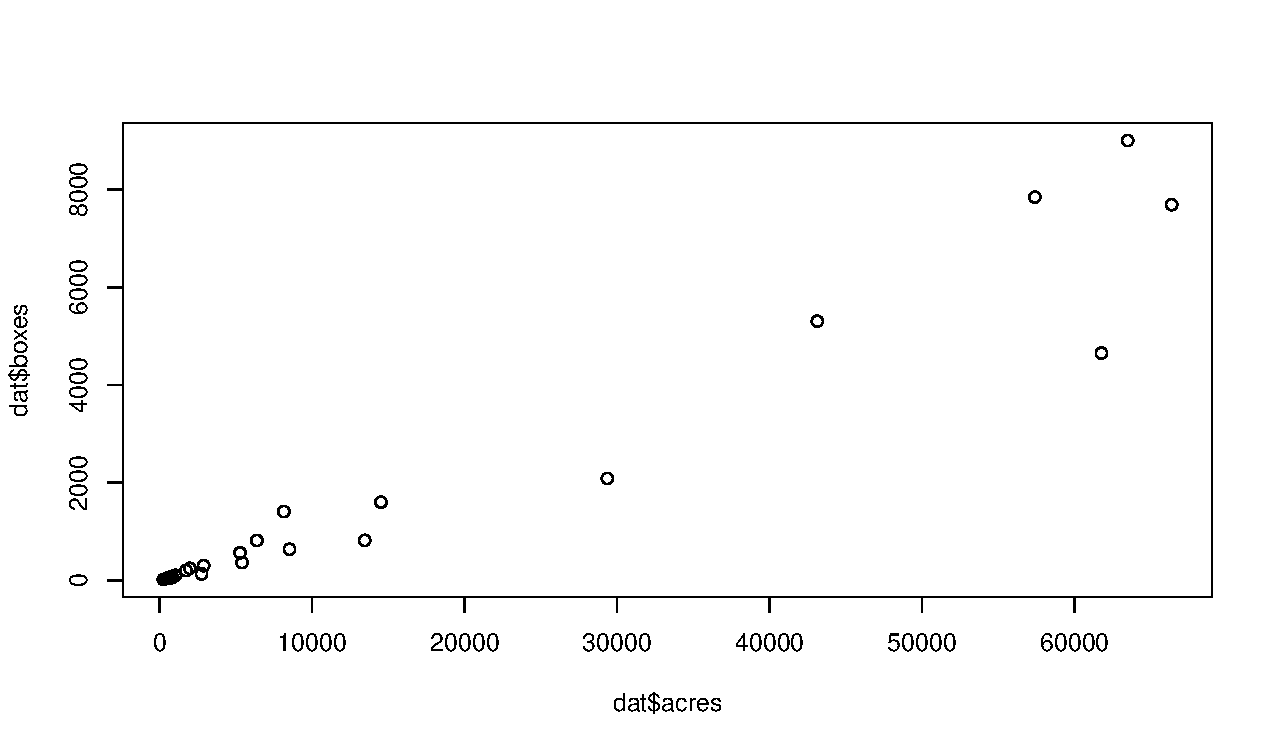
\includegraphics[width=\maxwidth]{figure/unnamed-chunk-54-1} 

}


\begin{kframe}\begin{alltt}
\hlstd{lm.1} \hlkwb{<-} \hlkwd{lm}\hlstd{(dat}\hlopt{$}\hlstd{boxes} \hlopt{~} \hlstd{dat}\hlopt{$}\hlstd{acres)}
\hlkwd{summary}\hlstd{(lm.1)}
\end{alltt}
\begin{verbatim}
## 
## Call:
## lm(formula = dat$boxes ~ dat$acres)
## 
## Residuals:
##      Min       1Q   Median       3Q      Max 
## -2470.81    -6.17    71.72   106.46  1677.32 
## 
## Coefficients:
##               Estimate Std. Error t value Pr(>|t|)    
## (Intercept) -85.391989 186.178031  -0.459    0.651    
## dat$acres     0.116717   0.006761  17.263 1.16e-14 ***
## ---
## Signif. codes:  0 '***' 0.001 '**' 0.01 '*' 0.05 '.' 0.1 ' ' 1
## 
## Residual standard error: 754.4 on 23 degrees of freedom
## Multiple R-squared:  0.9284,	Adjusted R-squared:  0.9252 
## F-statistic:   298 on 1 and 23 DF,  p-value: 1.164e-14
\end{verbatim}
\begin{alltt}
\hlcom{# Residual plot: vs fitted values.}
\hlkwd{plot}\hlstd{(lm.1}\hlopt{$}\hlstd{fitted.values,}
    \hlstd{lm.1}\hlopt{$}\hlstd{residuals,}
\hlkwc{xlab} \hlstd{=} \hlstr{"Fitted Values"}\hlstd{,}
\hlkwc{ylab} \hlstd{=} \hlstr{"Residuals"}\hlstd{)}
\end{alltt}
\end{kframe}

{\centering 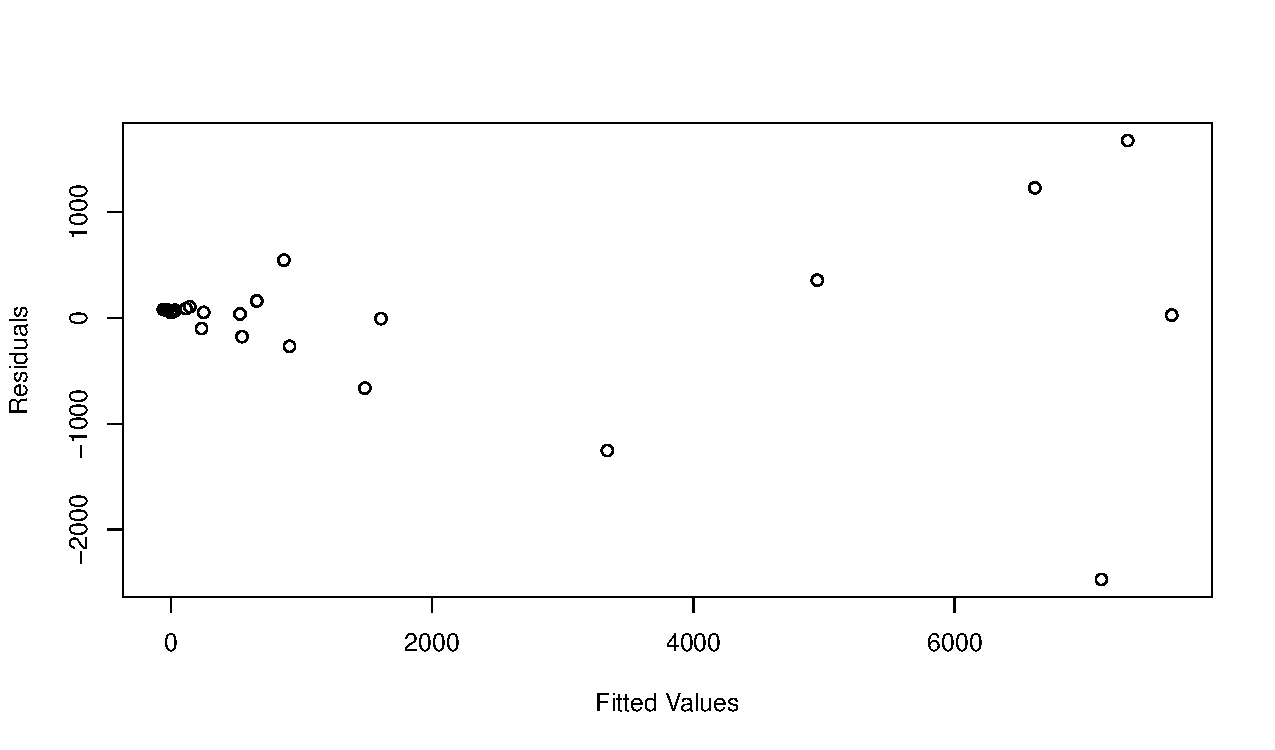
\includegraphics[width=\maxwidth]{figure/unnamed-chunk-54-2} 

}


\begin{kframe}\begin{alltt}
\hlcom{# Residual plot: vs predictor (just one in this case).}
\hlkwd{plot}\hlstd{(dat}\hlopt{$}\hlstd{acres, lm.1}\hlopt{$}\hlstd{residuals,} \hlkwc{xlab} \hlstd{=} \hlstr{"Acres"}\hlstd{,} \hlkwc{ylab} \hlstd{=} \hlstr{"Residuals"}\hlstd{)}
\end{alltt}
\end{kframe}

{\centering 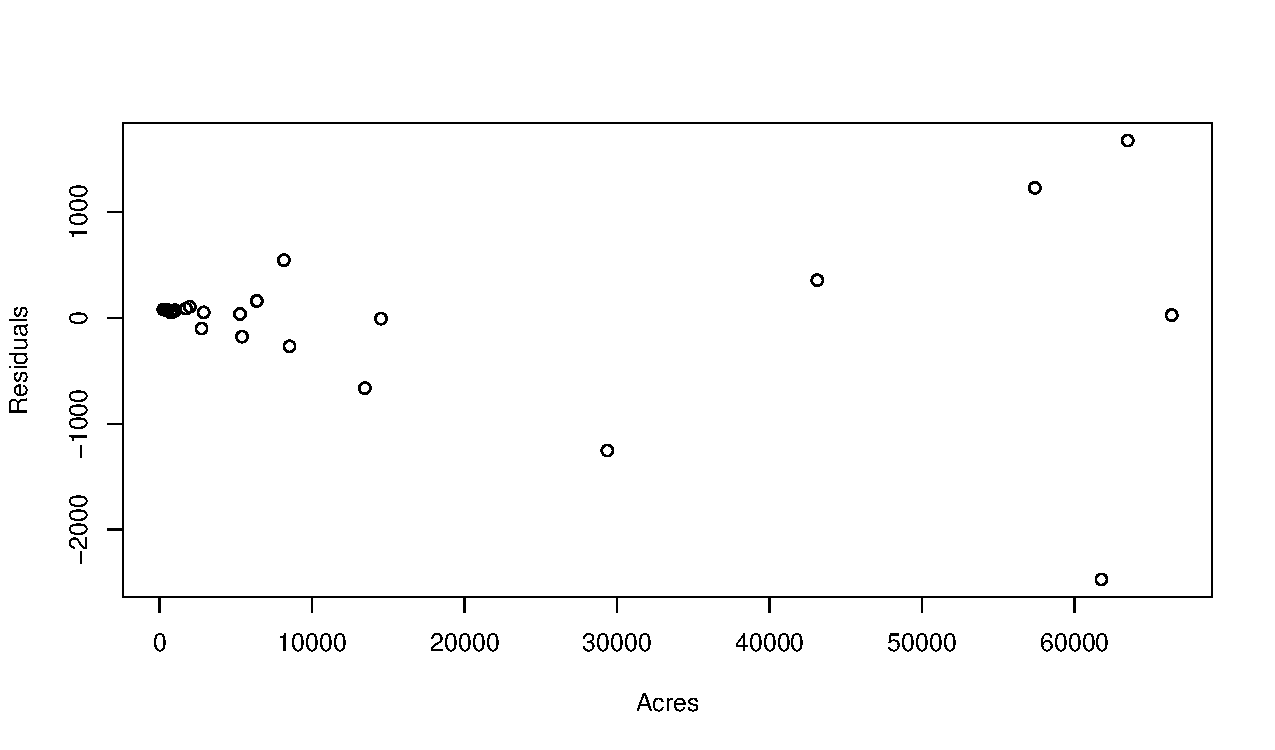
\includegraphics[width=\maxwidth]{figure/unnamed-chunk-54-3} 

}


\begin{kframe}\begin{alltt}
\hlcom{# Residual plot: vs i (just to demo plot; no time/space ordering here).}
\hlkwd{plot}\hlstd{(}\hlnum{1}\hlopt{:}\hlkwd{nrow}\hlstd{(dat), lm.1}\hlopt{$}\hlstd{residuals,} \hlkwc{xlab} \hlstd{=} \hlstr{"Index"}\hlstd{,} \hlkwc{ylab} \hlstd{=} \hlstr{"Residuals"}\hlstd{)}
\end{alltt}
\end{kframe}

{\centering 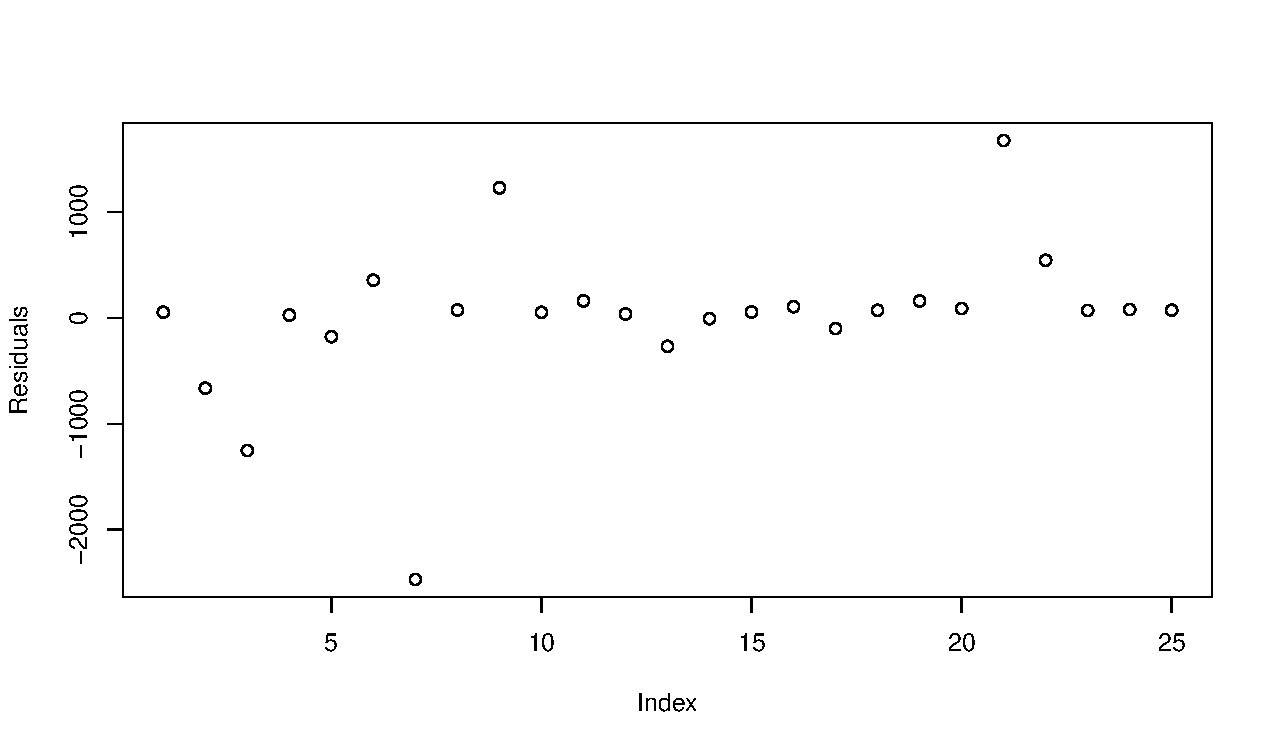
\includegraphics[width=\maxwidth]{figure/unnamed-chunk-54-4} 

}


\begin{kframe}\begin{alltt}
    \hlcom{# Histogram of residuals.}
    \hlkwd{hist}\hlstd{(lm.1}\hlopt{$}\hlstd{residuals)}
\end{alltt}
\end{kframe}

{\centering 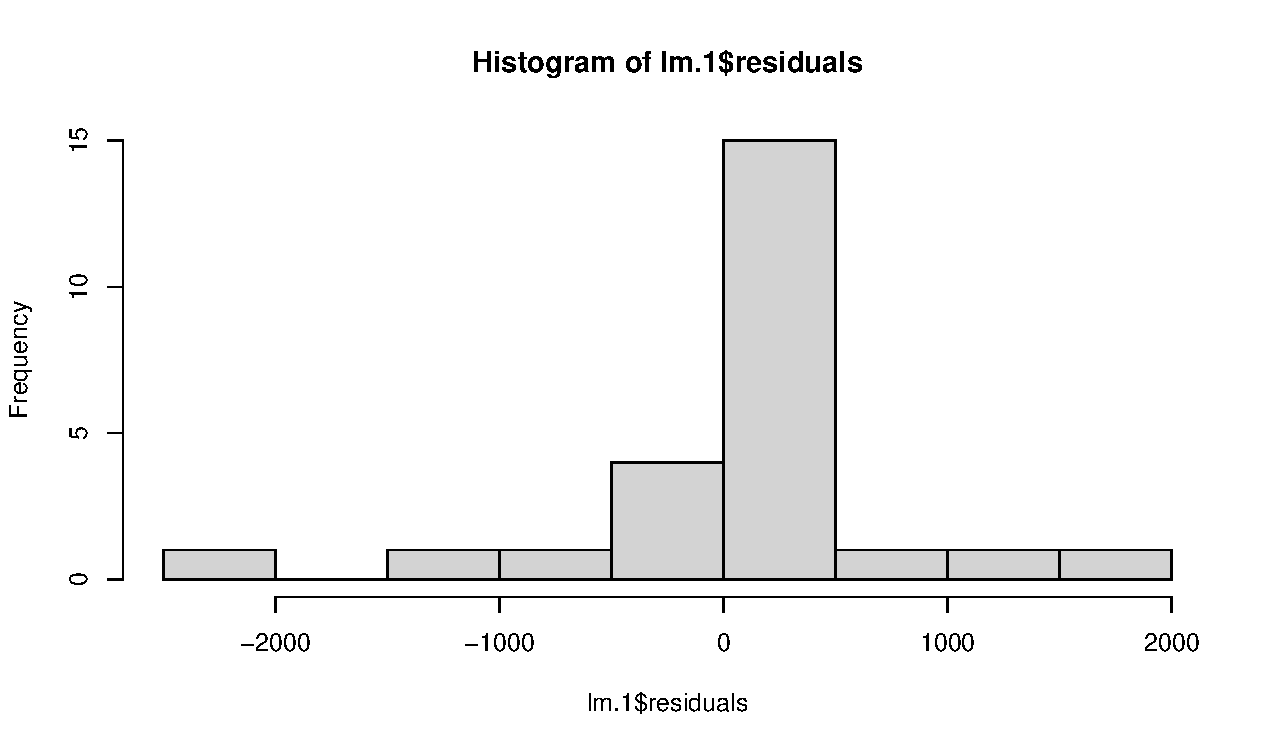
\includegraphics[width=\maxwidth]{figure/unnamed-chunk-54-5} 

}


\begin{kframe}\begin{alltt}
\hlcom{# QQ plot of residuals.}
\hlkwd{qqnorm}\hlstd{(lm.1}\hlopt{$}\hlstd{residuals)}
    \hlkwd{qqline}\hlstd{(lm.1}\hlopt{$}\hlstd{residuals,} \hlkwc{col} \hlstd{=} \hlstr{"blue"}\hlstd{,} \hlkwc{lwd} \hlstd{=} \hlnum{2}\hlstd{)}
\end{alltt}
\end{kframe}

{\centering 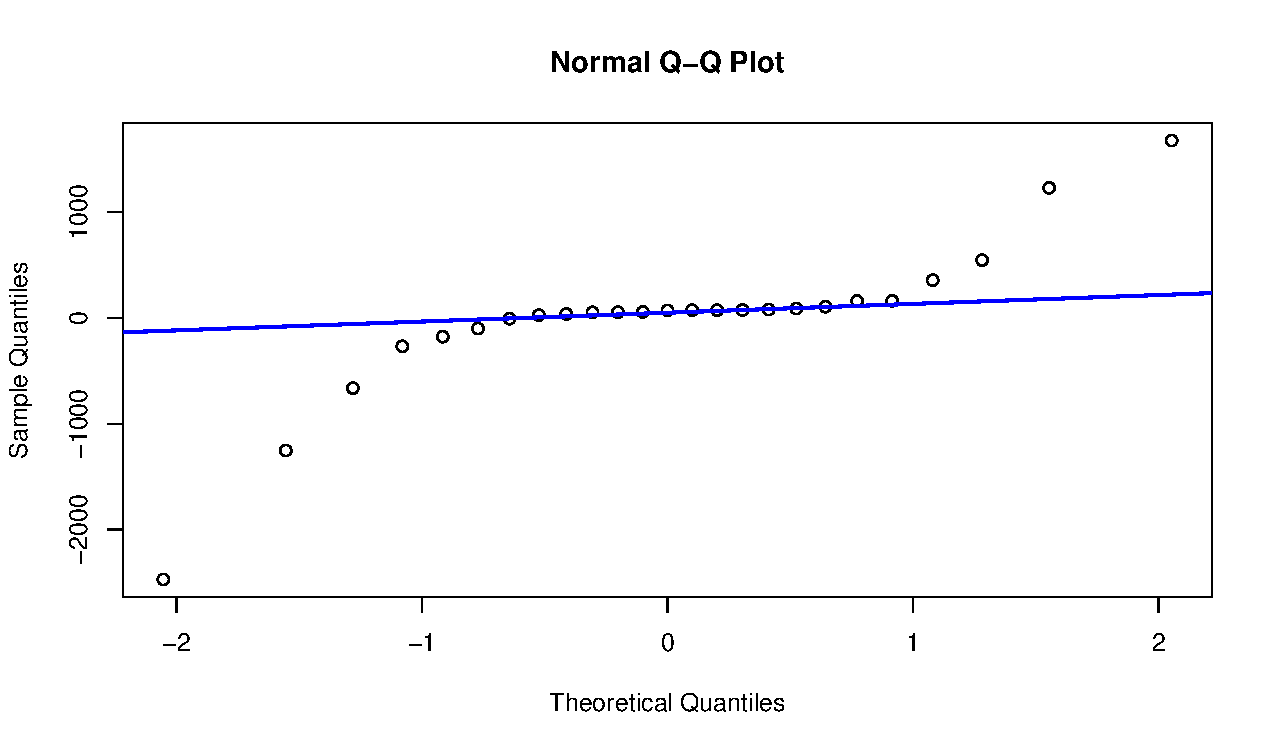
\includegraphics[width=\maxwidth]{figure/unnamed-chunk-54-6} 

}


\begin{kframe}\begin{alltt}
\hlcom{## Rocket data revisited.}
\hlstd{rocket} \hlkwb{<-} \hlkwd{read.csv}\hlstd{(}\hlstr{"csv/rocket.csv"}\hlstd{)}
\hlstd{mr} \hlkwb{<-} \hlkwd{lm}\hlstd{(thrust} \hlopt{~} \hlstd{nozzle} \hlopt{+} \hlstd{propratio,} \hlkwc{data} \hlstd{= rocket)}
\hlkwd{summary}\hlstd{(mr)}
\end{alltt}
\begin{verbatim}
## 
## Call:
## lm(formula = thrust ~ nozzle + propratio, data = rocket)
## 
## Residuals:
##     Min      1Q  Median      3Q     Max 
## -3.8459 -1.7555  0.5934  1.2906  3.3008 
## 
## Coefficients:
##             Estimate Std. Error t value Pr(>|t|)    
## (Intercept) 473.6039     4.7158 100.430 4.88e-15 ***
## nozzle       16.7383     1.5329  10.919 1.71e-06 ***
## propratio    -1.0948     0.9414  -1.163    0.275    
## ---
## Signif. codes:  0 '***' 0.001 '**' 0.01 '*' 0.05 '.' 0.1 ' ' 1
## 
## Residual standard error: 2.655 on 9 degrees of freedom
## Multiple R-squared:  0.9303,	Adjusted R-squared:  0.9148 
## F-statistic: 60.05 on 2 and 9 DF,  p-value: 6.238e-06
\end{verbatim}
\begin{alltt}
\hlcom{# Residual plot: vs fitted values.}
\hlkwd{plot}\hlstd{(mr}\hlopt{$}\hlstd{fitted.values,}
    \hlstd{mr}\hlopt{$}\hlstd{residuals,}
\hlkwc{xlab} \hlstd{=} \hlstr{"Fitted Values"}\hlstd{,}
\hlkwc{ylab} \hlstd{=} \hlstr{"Residuals"}\hlstd{)}
\end{alltt}
\end{kframe}

{\centering 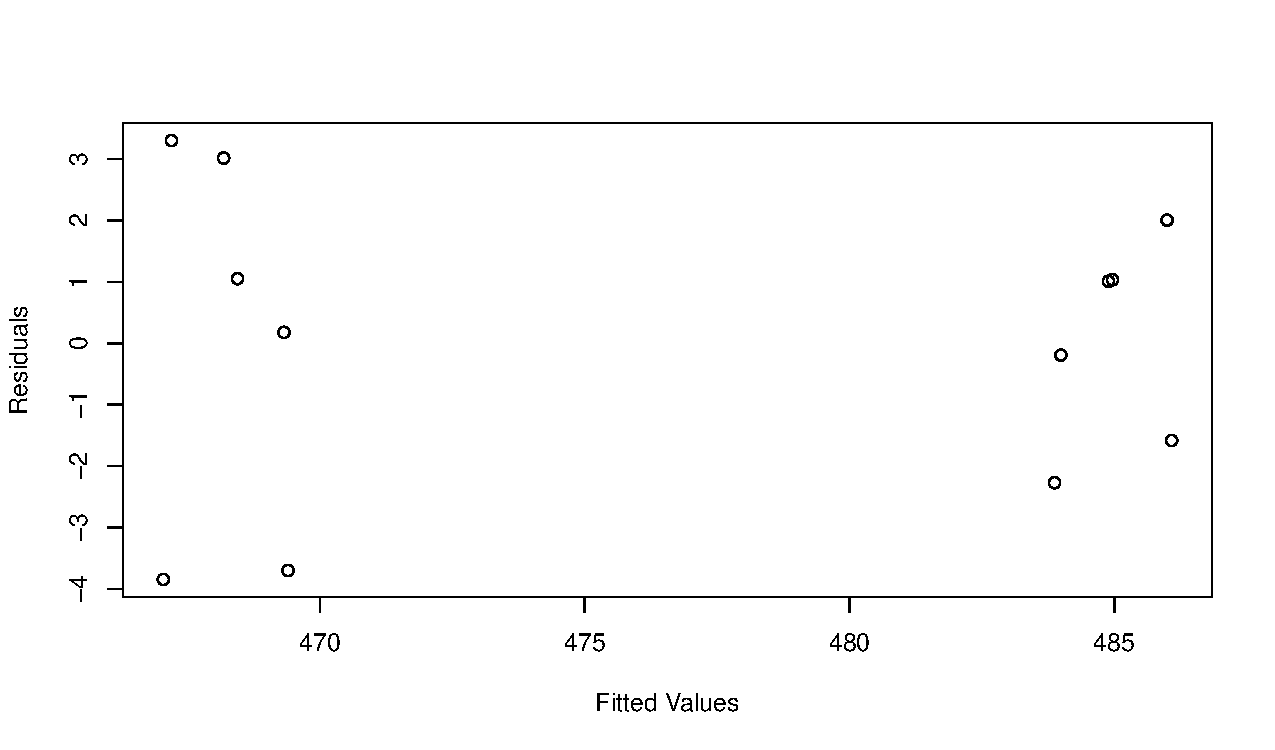
\includegraphics[width=\maxwidth]{figure/unnamed-chunk-54-7} 

}


\begin{kframe}\begin{alltt}
\hlcom{# Residual plot: vs predictors.}
\hlkwd{plot}\hlstd{(rocket}\hlopt{$}\hlstd{nozzle, mr}\hlopt{$}\hlstd{residuals,} \hlkwc{xlab} \hlstd{=} \hlstr{"Nozzle (1 = large)"}\hlstd{,}
\hlkwc{ylab} \hlstd{=} \hlstr{"Residuals"}\hlstd{)}
\end{alltt}
\end{kframe}

{\centering 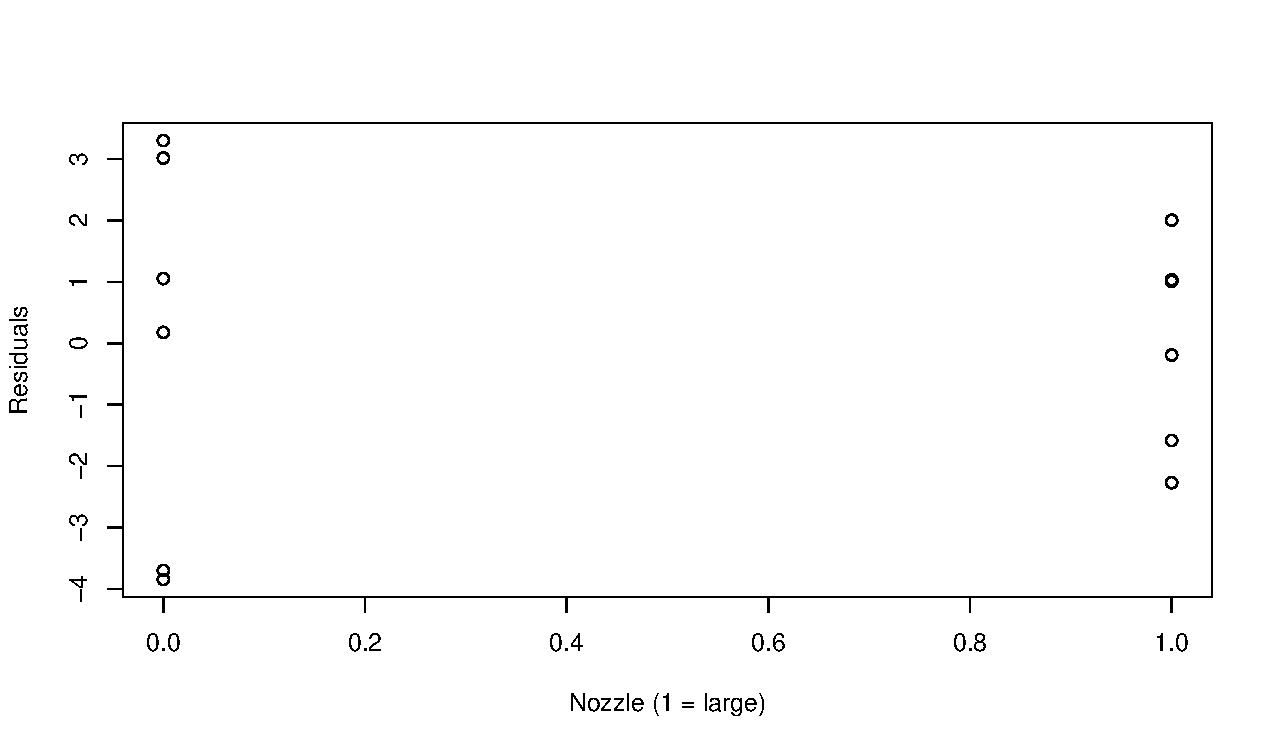
\includegraphics[width=\maxwidth]{figure/unnamed-chunk-54-8} 

}


\begin{kframe}\begin{alltt}
\hlkwd{plot}\hlstd{(rocket}\hlopt{$}\hlstd{propratio,}
    \hlstd{mr}\hlopt{$}\hlstd{residuals,}
\hlkwc{xlab} \hlstd{=} \hlstr{"Propellant to fuel ratio"}\hlstd{,}
\hlkwc{ylab} \hlstd{=} \hlstr{"Residuals"}\hlstd{)}
\end{alltt}
\end{kframe}

{\centering 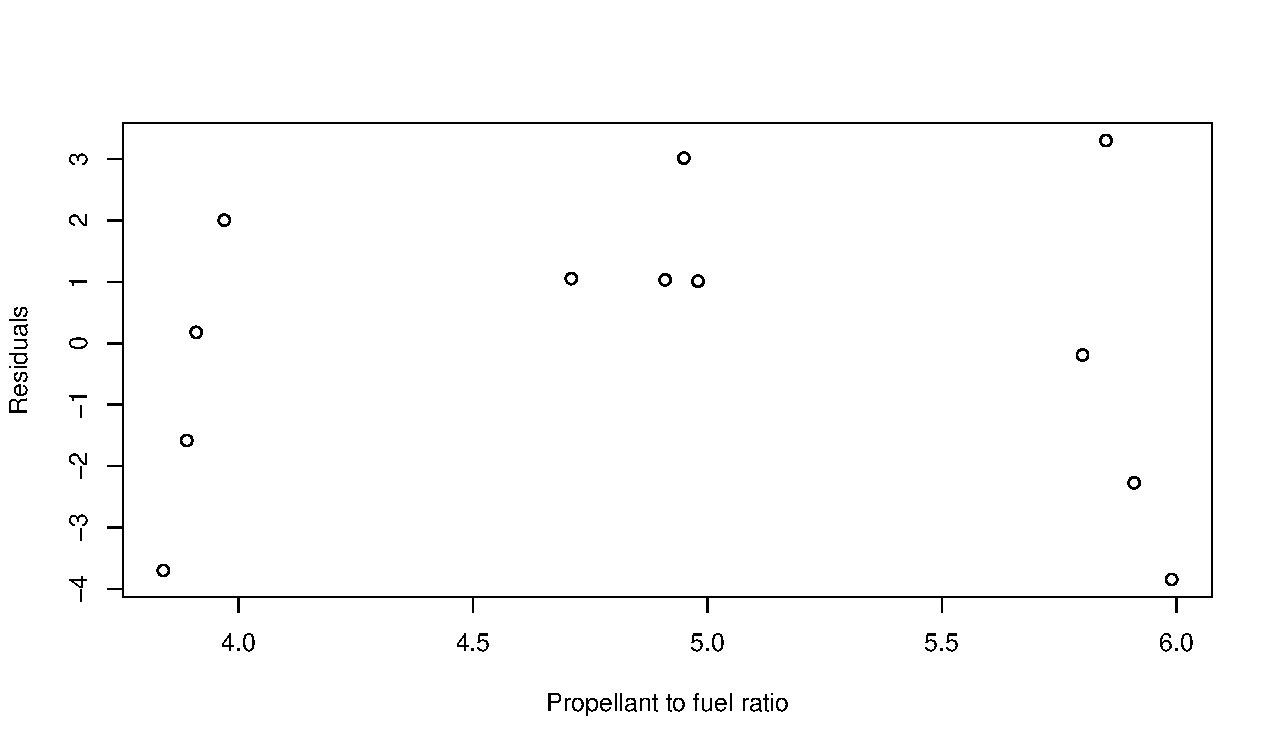
\includegraphics[width=\maxwidth]{figure/unnamed-chunk-54-9} 

}


\begin{kframe}\begin{alltt}
\hlcom{# Histogram of residuals,}
\hlkwd{hist}\hlstd{(mr}\hlopt{$}\hlstd{residuals)}
\end{alltt}
\end{kframe}

{\centering 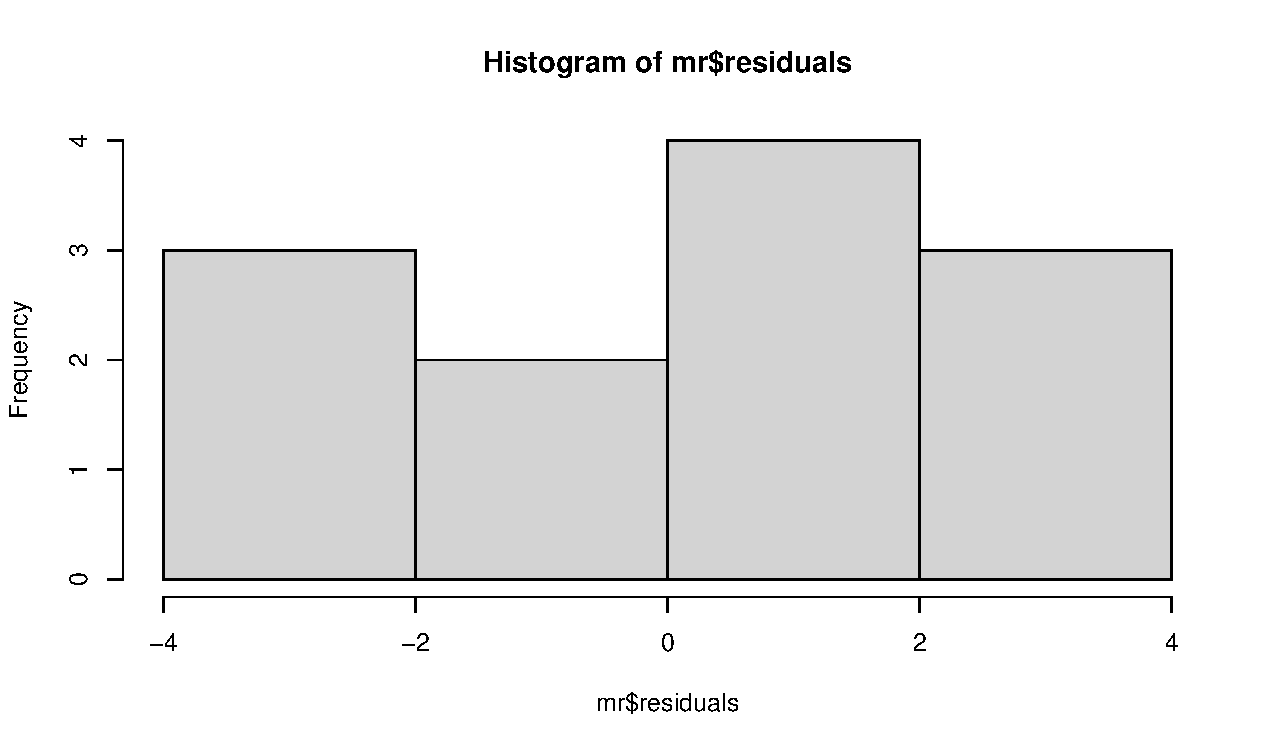
\includegraphics[width=\maxwidth]{figure/unnamed-chunk-54-10} 

}


\begin{kframe}\begin{alltt}
    \hlcom{# QQ plot of residuals,}
    \hlkwd{qqnorm}\hlstd{(mr}\hlopt{$}\hlstd{residuals)}
\hlkwd{qqline}\hlstd{(mr}\hlopt{$}\hlstd{residuals,} \hlkwc{col} \hlstd{=} \hlstr{"blue"}\hlstd{,} \hlkwc{lwd} \hlstd{=} \hlnum{2}\hlstd{)}
\end{alltt}
\end{kframe}

{\centering 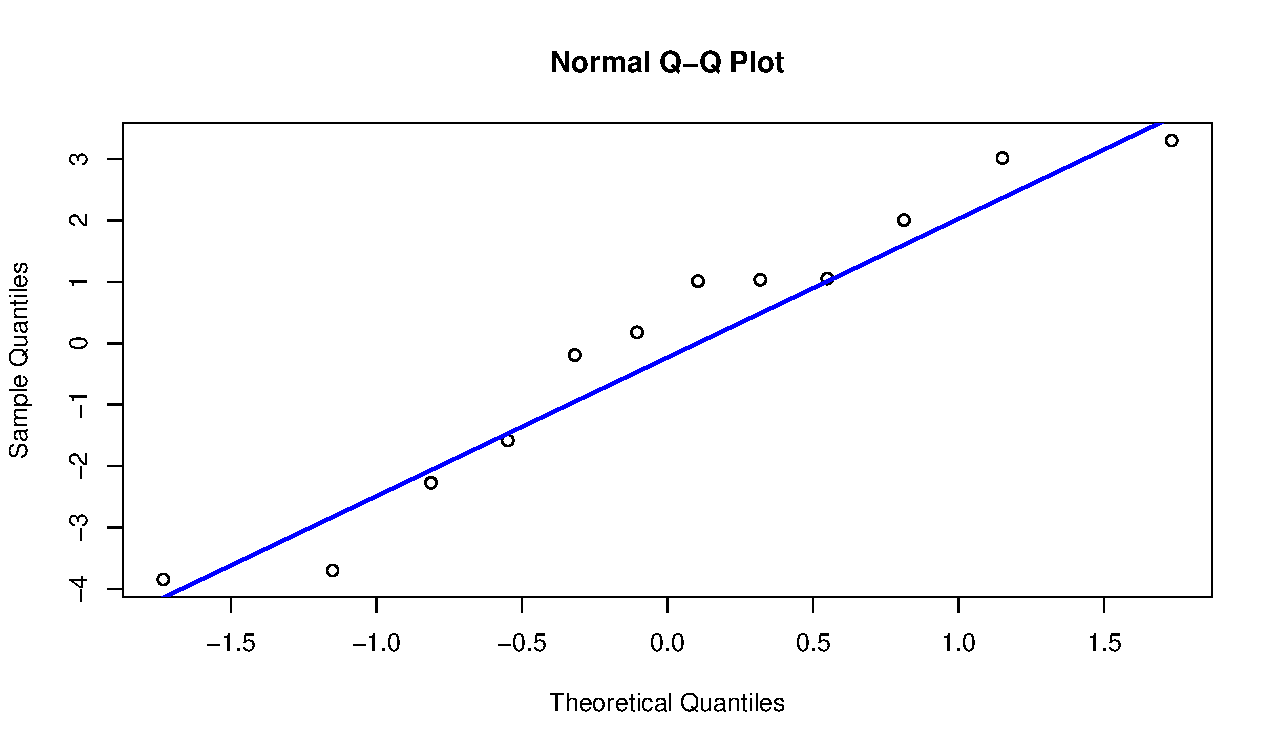
\includegraphics[width=\maxwidth]{figure/unnamed-chunk-54-11} 

}


\end{knitrout}
\section{2020-02-10}
\underline{Roadmap}:
\begin{itemize}
    \item Interval Estimation
          \subitem Likelihood Estimation
          \subitem Confidence Intervals: Coverage probabilities, Pivotal Quantities
\end{itemize}
\begin{exbox}
    \begin{example}
        The approval rating of Trump is $ 49\% $ ($ 49\% $ is the most ``likely'' value of $ \theta $)
        where $ \theta= $ population approval rating.
        \begin{itemize}
            \item What is the ``Margin of Error''?
                  \subitem How does one calculate it?
        \end{itemize}
    \end{example}
\end{exbox}
\underline{Setup} $ Y_1,\ldots ,Y_n $ are iid random variables with
distribution (density) $ f(y;\theta) $ where $ \theta= $ unknown attribute.

\underline{Objective}: Based on our data $ \{y_1,\ldots ,y_n\} $, we would
construct an interval $ [a,b] $
\[ a(y_1,\ldots ,y_n),b(y_1,\ldots ,y_n) \]
which are the ``reasonable'' values of $ \theta $.

\underline{Method 1}: Through the relative likelihood function.

\underline{Intuition}: $ \theta $ is ``reasonable'' of $ L(\theta) $
is ``close'' to $ L(\hat{\theta}) $, where $ \theta= $ MLE.

\begin{defbox}
    \begin{definition}
        A $ 100p\% $ likelihood interval for $ \theta $ where $ p\in[0,1] $
        \[ \{\theta:R(\theta)\geqslant p\} \]
    \end{definition}
\end{defbox}
Take $ p=0.5 $, we get that $ R(\theta)\geqslant 0.5 $, so
\[ \implies L(\theta)\geqslant 0.5 L(\hat{\theta}) \]
The value of the likelihood at $ \theta $ is at least $ 50\% $ of the value of the
likelihood evaluated at the MLE.

\underline{Convention}
\begin{itemize}
    \item $ R(\theta)\geqslant 0.5\implies \theta $ is very plausible
    \item $ 0.1\leqslant R(\theta)<0.5\implies \theta $ is plausible
    \item $ 0.01\leqslant R(\theta)<0.1\implies \theta $ is implausible
    \item $ R(\theta)<0.01\implies \theta $ is very implausible
\end{itemize}
\begin{exbox}
    \begin{example}
        A coin is tossed $ 200 $ times and we observe $ 120 $ heads.
        Let $ \theta=P(\text{H}) $. Is $ \theta=0.5 $ plausible?

        \textbf{Solution.} Find the $ 10\% $ likelihood interval for $ \theta $.
        \[ L(\theta)=\binom{200}{120}\theta^{120}(1-\theta)^{80} \]
        We are given that $ \hat{\theta}=0.6 $.
        \[ \left\{ \theta:\frac{\theta^{120}(1-\theta)^{80}}{0.6^{120}(0.4)^{80}}\geqslant 0.1 \right\} \]
        Thus,
        \[ R(\theta)=\frac{\theta^{120}(1-\theta)^{80}}{0.6^{120}(0.4)^{80}} \]
        Is $ \theta=0.5 $ plausible? Plug in $ \theta=0.5 $ and check if $ R(0.5)\geqslant 0.1 $.
    \end{example}
\end{exbox}
\begin{exbox}
    \begin{example}
        Two Binomial experiments.
        \begin{itemize}
            \item $ n_1=1000 $, $ y_1=200 $
            \item $ n_2=100 $, $ y_2=20 $
            \item $ y= $ number of successes
            \item $ n= $ number of trials
        \end{itemize}
        Which $ 10\% $ likelihood interval is wider?

        \textbf{Solution.} We have $ \hat{\theta}=0.2 $.
        $ n=100 $ yields a wider interval.
    \end{example}
\end{exbox}

\underline{Method 2}: Confidence intervals.

\underline{Setup}: There is a pre-specified probability (coverage probability),
say $ 95\% $ or $ 99\% $ for example.

\underline{Objective}: Based on your data, we want to estimate the (random)
interval which would contain $ \theta $ with that probability.
\begin{exbox}
    \begin{example}
        The STAT 231 scores of UW Math students is normally distributed independently
        \[ Y_i \thicksim N(\mu,64) \]
        A sample of $ 25 $ students are collected
        \[ \bar{y}=75 \]
        Find the $ 95\% $ confidence interval for $ \mu $.
    \end{example}
\end{exbox}
\underline{Sampling Distributions}

\underline{Idea}: All the data summaries are also outcomes of some random experiment.
\[ Y_1,\ldots ,Y_n \thicksim N(\mu,\sigma^2) \quad\text{iid}\]
\[ \implies \bar{Y} \thicksim N(\mu,\sigma^2/n) \]
Our sample mean $ \bar{y} $ is an outcome of this experiment.


\subsection{R Demo}
\begin{knitrout}
\definecolor{shadecolor}{rgb}{0.969, 0.969, 0.969}\color{fgcolor}\begin{kframe}
\begin{alltt}
\hlkwd{library}\hlstd{(MASS)}
\hlcom{## Demo for transformations and interactions}

\hlcom{## Florida oranges revisited}
\hlstd{dat} \hlkwb{<-} \hlkwd{read.csv}\hlstd{(}\hlstr{"csv/florange.csv"}\hlstd{)}
\hlstd{lm.1} \hlkwb{<-} \hlkwd{lm}\hlstd{(dat}\hlopt{$}\hlstd{boxes} \hlopt{~} \hlstd{dat}\hlopt{$}\hlstd{acres)}
\hlkwd{summary}\hlstd{(lm.1)}
\end{alltt}
\begin{verbatim}
## 
## Call:
## lm(formula = dat$boxes ~ dat$acres)
## 
## Residuals:
##      Min       1Q   Median       3Q      Max 
## -2470.81    -6.17    71.72   106.46  1677.32 
## 
## Coefficients:
##               Estimate Std. Error t value Pr(>|t|)    
## (Intercept) -85.391989 186.178031  -0.459    0.651    
## dat$acres     0.116717   0.006761  17.263 1.16e-14 ***
## ---
## Signif. codes:  0 '***' 0.001 '**' 0.01 '*' 0.05 '.' 0.1 ' ' 1
## 
## Residual standard error: 754.4 on 23 degrees of freedom
## Multiple R-squared:  0.9284,	Adjusted R-squared:  0.9252 
## F-statistic:   298 on 1 and 23 DF,  p-value: 1.164e-14
\end{verbatim}
\begin{alltt}
\hlcom{# Recall: residuals had non-constant variance}
\hlcom{#  (variance increases with fitted values)}
\hlkwd{plot}\hlstd{(lm.1}\hlopt{$}\hlstd{fitted.values,}
      \hlstd{lm.1}\hlopt{$}\hlstd{residuals,}
\hlkwc{xlab} \hlstd{=} \hlstr{"Fitted Values"}\hlstd{,}
\hlkwc{ylab} \hlstd{=} \hlstr{"Residuals"}\hlstd{)}
\end{alltt}
\end{kframe}

{\centering 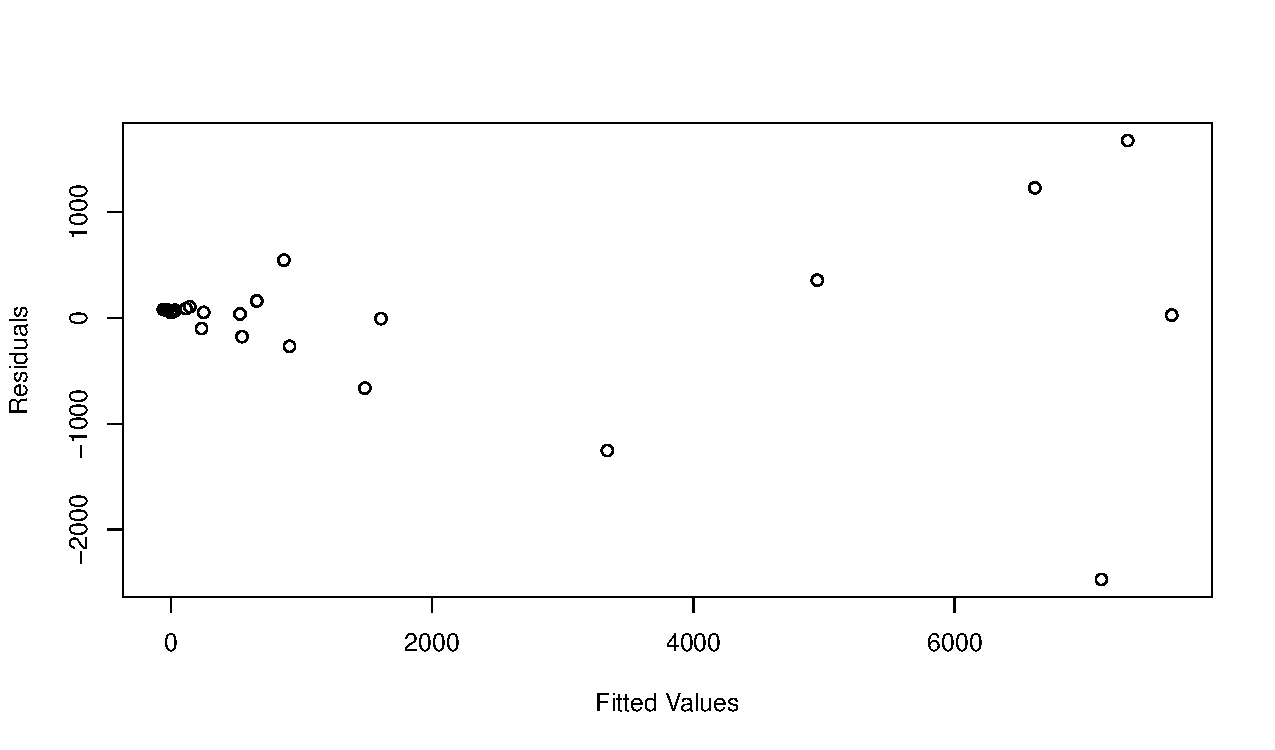
\includegraphics[width=\maxwidth]{figure/unnamed-chunk-55-1} 

}


\begin{kframe}\begin{alltt}
\hlkwd{qqnorm}\hlstd{(lm.1}\hlopt{$}\hlstd{residuals)}
      \hlkwd{qqline}\hlstd{(lm.1}\hlopt{$}\hlstd{residuals,} \hlkwc{col} \hlstd{=} \hlstr{"blue"}\hlstd{,} \hlkwc{lwd} \hlstd{=} \hlnum{2}\hlstd{)}
\end{alltt}
\end{kframe}

{\centering 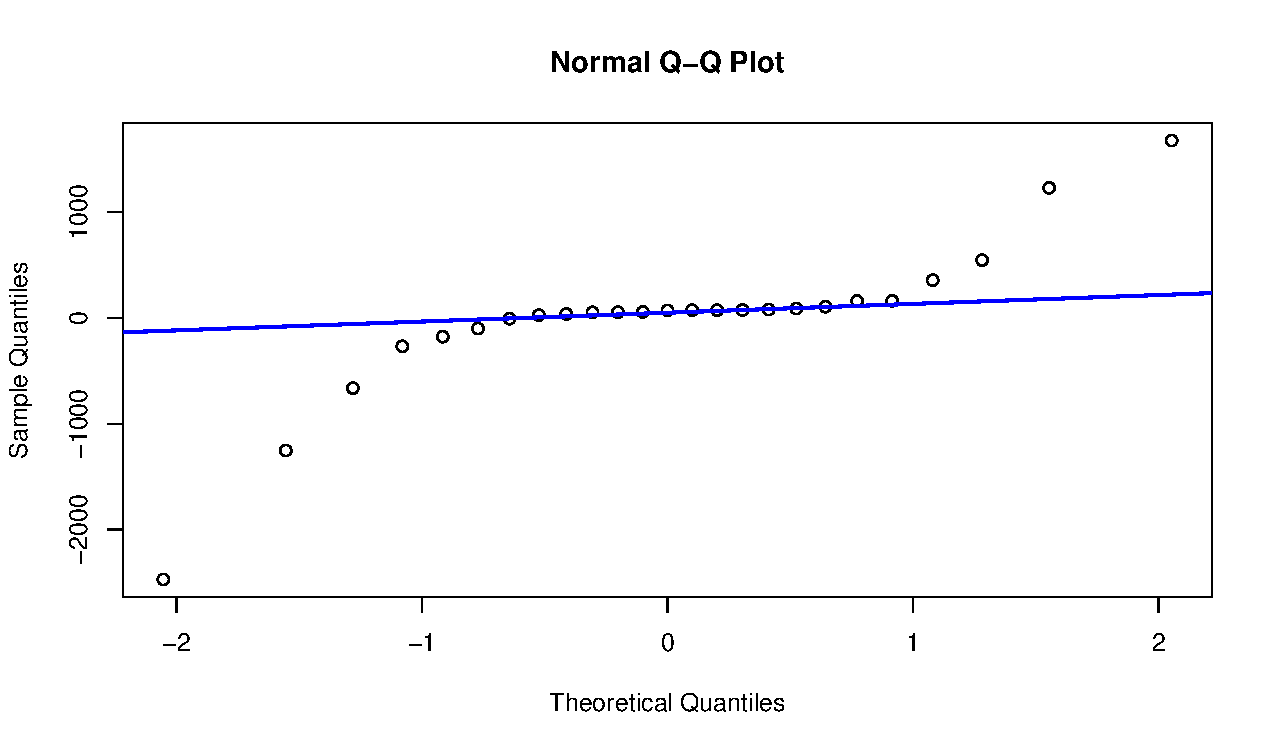
\includegraphics[width=\maxwidth]{figure/unnamed-chunk-55-2} 

}


\begin{kframe}\begin{alltt}
\hlcom{# Try log-transforming y}
\hlstd{lm.log} \hlkwb{<-} \hlkwd{lm}\hlstd{(}\hlkwd{log}\hlstd{(dat}\hlopt{$}\hlstd{boxes)} \hlopt{~} \hlstd{dat}\hlopt{$}\hlstd{acres)}
\hlkwd{summary}\hlstd{(lm.log)}
\end{alltt}
\begin{verbatim}
## 
## Call:
## lm(formula = log(dat$boxes) ~ dat$acres)
## 
## Residuals:
##     Min      1Q  Median      3Q     Max 
## -2.0175 -0.7767  0.1142  0.7106  1.6102 
## 
## Coefficients:
##              Estimate Std. Error t value Pr(>|t|)    
## (Intercept) 5.093e+00  2.425e-01  20.997  < 2e-16 ***
## dat$acres   6.748e-05  8.808e-06   7.661 8.95e-08 ***
## ---
## Signif. codes:  0 '***' 0.001 '**' 0.01 '*' 0.05 '.' 0.1 ' ' 1
## 
## Residual standard error: 0.9828 on 23 degrees of freedom
## Multiple R-squared:  0.7184,	Adjusted R-squared:  0.7062 
## F-statistic: 58.69 on 1 and 23 DF,  p-value: 8.948e-08
\end{verbatim}
\begin{alltt}
\hlkwd{plot}\hlstd{(lm.log}\hlopt{$}\hlstd{fitted.values,}
      \hlstd{lm.log}\hlopt{$}\hlstd{residuals,}
\hlkwc{xlab} \hlstd{=} \hlstr{"Fitted Values"}\hlstd{,}
\hlkwc{ylab} \hlstd{=} \hlstr{"Residuals"}\hlstd{)}
\end{alltt}
\end{kframe}

{\centering 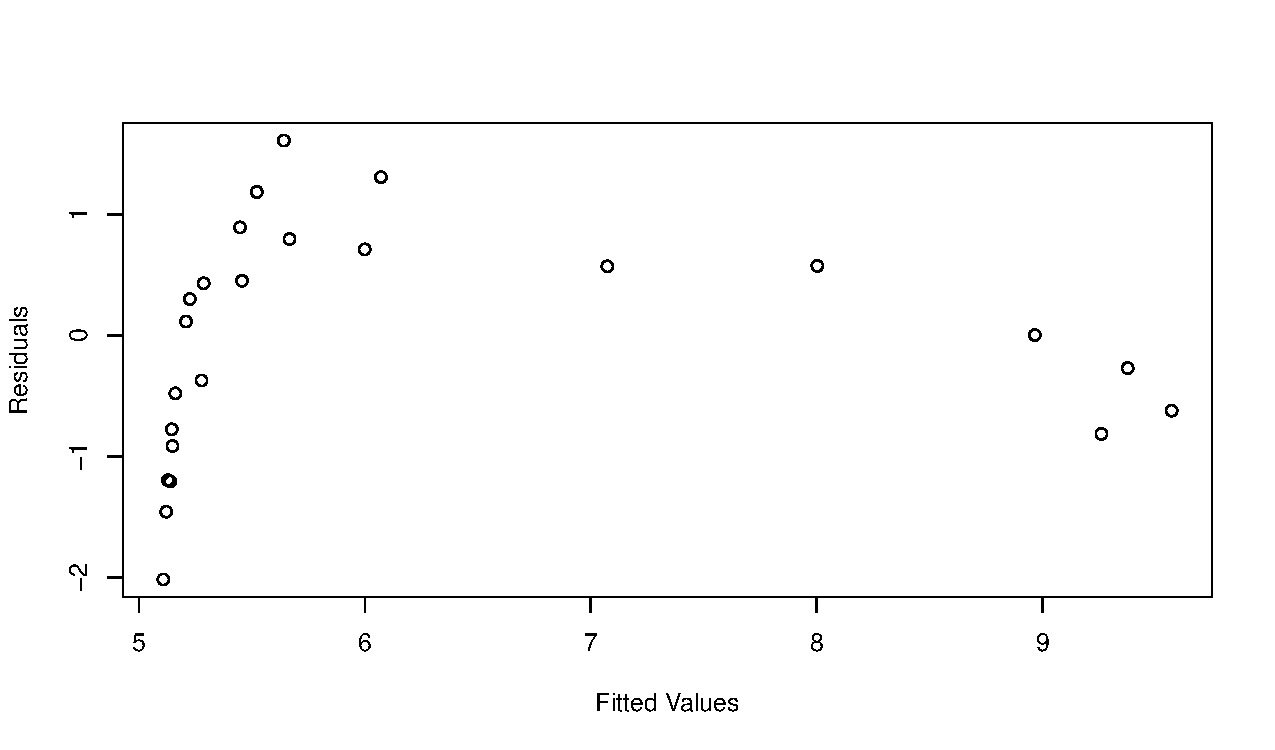
\includegraphics[width=\maxwidth]{figure/unnamed-chunk-55-3} 

}


\begin{kframe}\begin{alltt}
\hlkwd{plot}\hlstd{(dat}\hlopt{$}\hlstd{acres, lm.log}\hlopt{$}\hlstd{residuals,} \hlkwc{xlab} \hlstd{=} \hlstr{"Fitted Values"}\hlstd{,} \hlkwc{ylab} \hlstd{=} \hlstr{"Residuals"}\hlstd{)}
\end{alltt}
\end{kframe}

{\centering 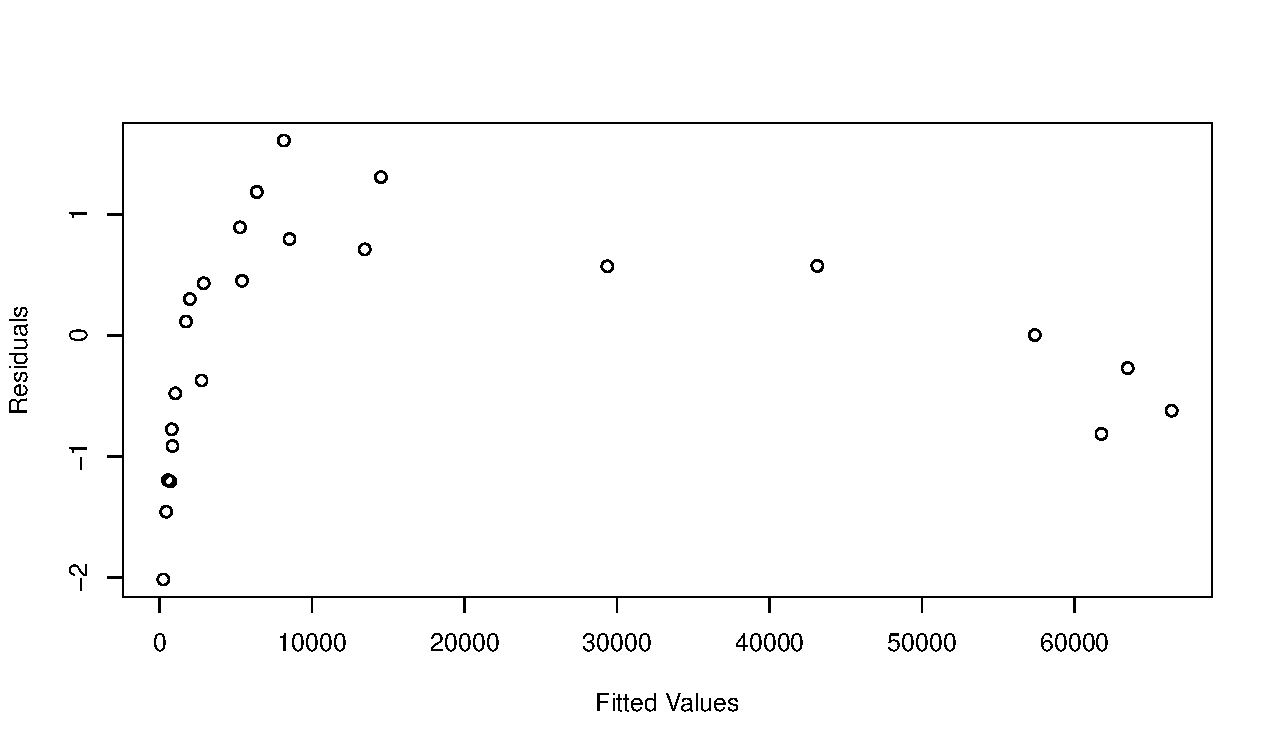
\includegraphics[width=\maxwidth]{figure/unnamed-chunk-55-4} 

}


\begin{kframe}\begin{alltt}
\hlkwd{qqnorm}\hlstd{(lm.log}\hlopt{$}\hlstd{residuals)}
      \hlkwd{qqline}\hlstd{(lm.log}\hlopt{$}\hlstd{residuals,} \hlkwc{col} \hlstd{=} \hlstr{"blue"}\hlstd{,} \hlkwc{lwd} \hlstd{=} \hlnum{2}\hlstd{)}
\end{alltt}
\end{kframe}

{\centering 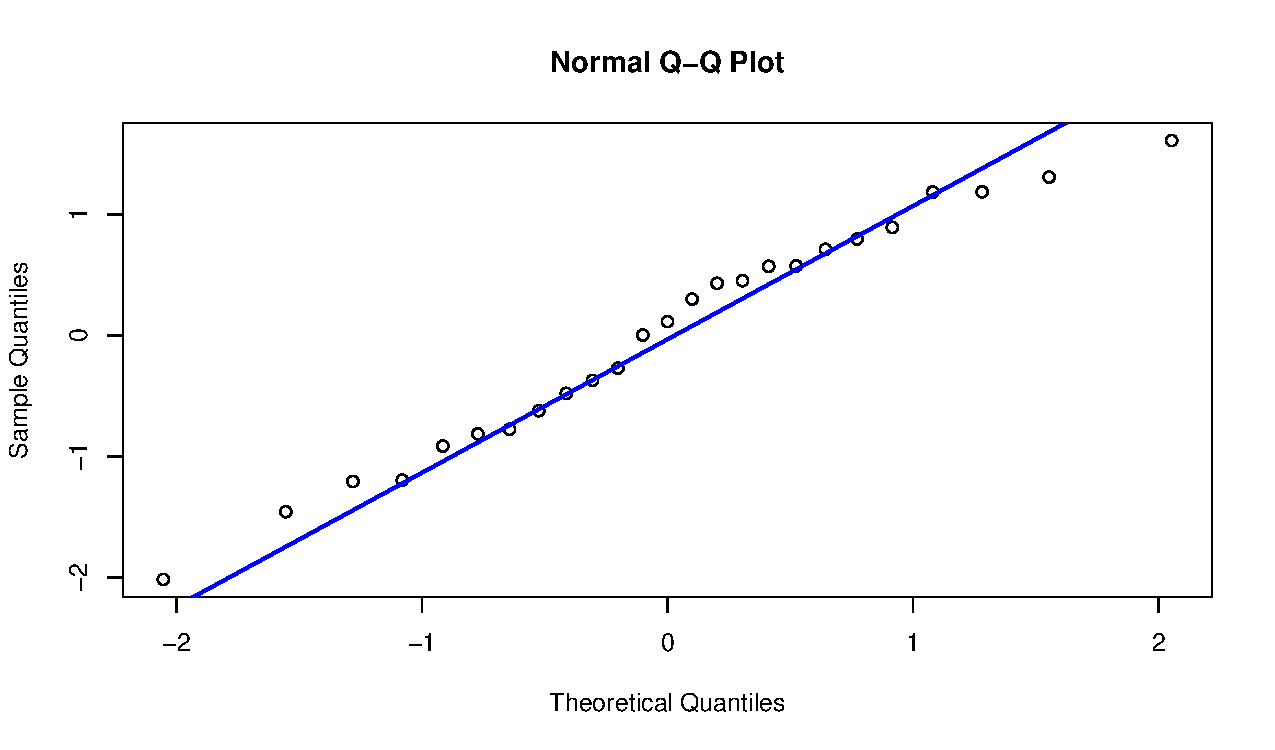
\includegraphics[width=\maxwidth]{figure/unnamed-chunk-55-5} 

}


\begin{kframe}\begin{alltt}
\hlcom{# Does the plot of residuals vs x suggest a problem}
\hlcom{# Let's take a closer look}
\hlkwd{plot}\hlstd{(dat}\hlopt{$}\hlstd{acres,} \hlkwd{log}\hlstd{(dat}\hlopt{$}\hlstd{boxes))} \hlcom{# evidently not linear!}
\end{alltt}
\end{kframe}

{\centering 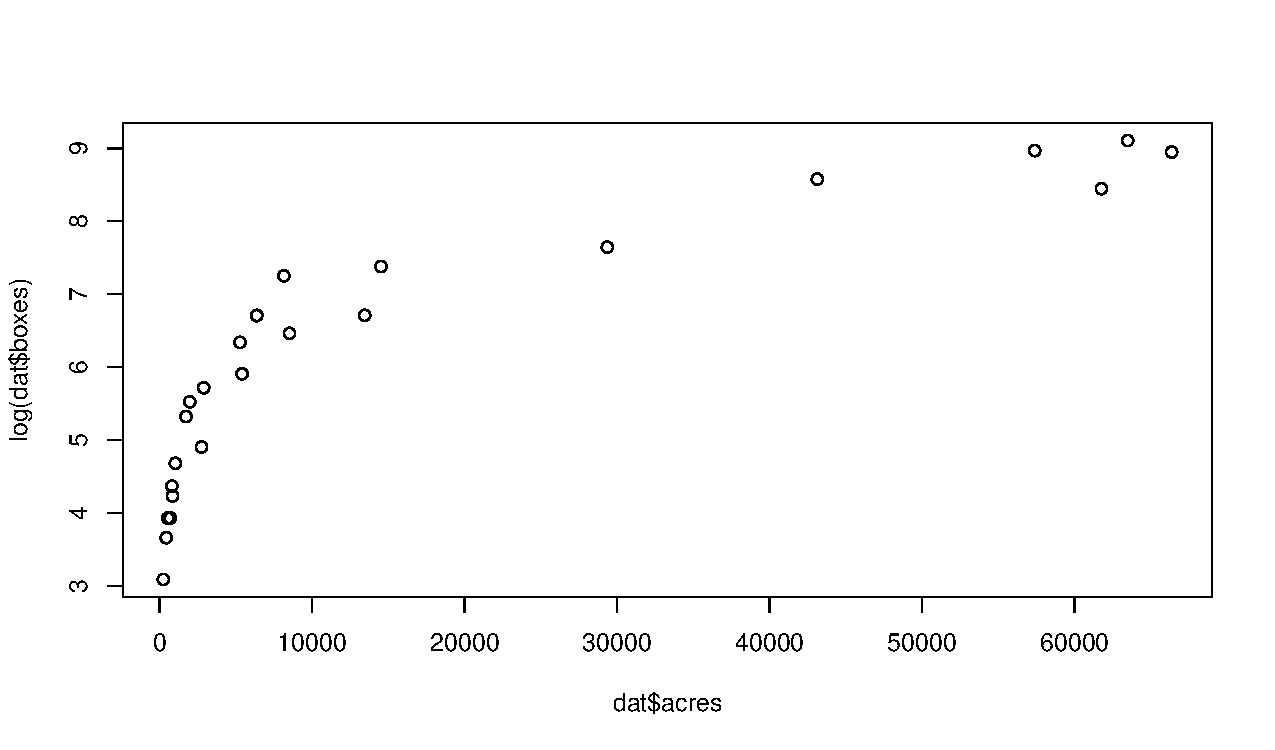
\includegraphics[width=\maxwidth]{figure/unnamed-chunk-55-6} 

}


\begin{kframe}\begin{alltt}
\hlcom{# Log-transform x as well}
\hlkwd{plot}\hlstd{(}\hlkwd{log}\hlstd{(dat}\hlopt{$}\hlstd{acres),} \hlkwd{log}\hlstd{(dat}\hlopt{$}\hlstd{boxes))} \hlcom{# looks much more linear!}
\end{alltt}
\end{kframe}

{\centering 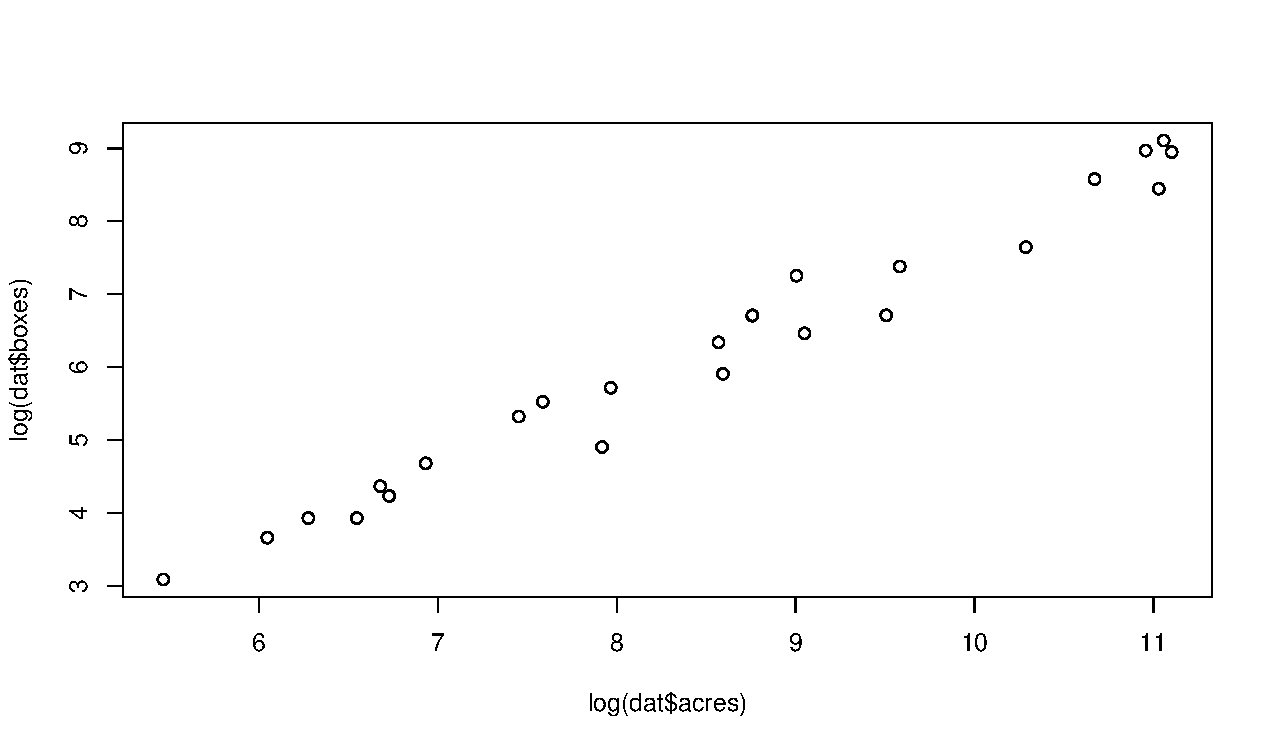
\includegraphics[width=\maxwidth]{figure/unnamed-chunk-55-7} 

}


\begin{kframe}\begin{alltt}
\hlstd{lm.loglog} \hlkwb{<-} \hlkwd{lm}\hlstd{(}\hlkwd{log}\hlstd{(dat}\hlopt{$}\hlstd{boxes)} \hlopt{~} \hlkwd{log}\hlstd{(dat}\hlopt{$}\hlstd{acres))}
\hlkwd{qqnorm}\hlstd{(lm.loglog}\hlopt{$}\hlstd{residuals)}
      \hlkwd{qqline}\hlstd{(lm.loglog}\hlopt{$}\hlstd{residuals,} \hlkwc{col} \hlstd{=} \hlstr{"blue"}\hlstd{,} \hlkwc{lwd} \hlstd{=} \hlnum{2}\hlstd{)}
\end{alltt}
\end{kframe}

{\centering 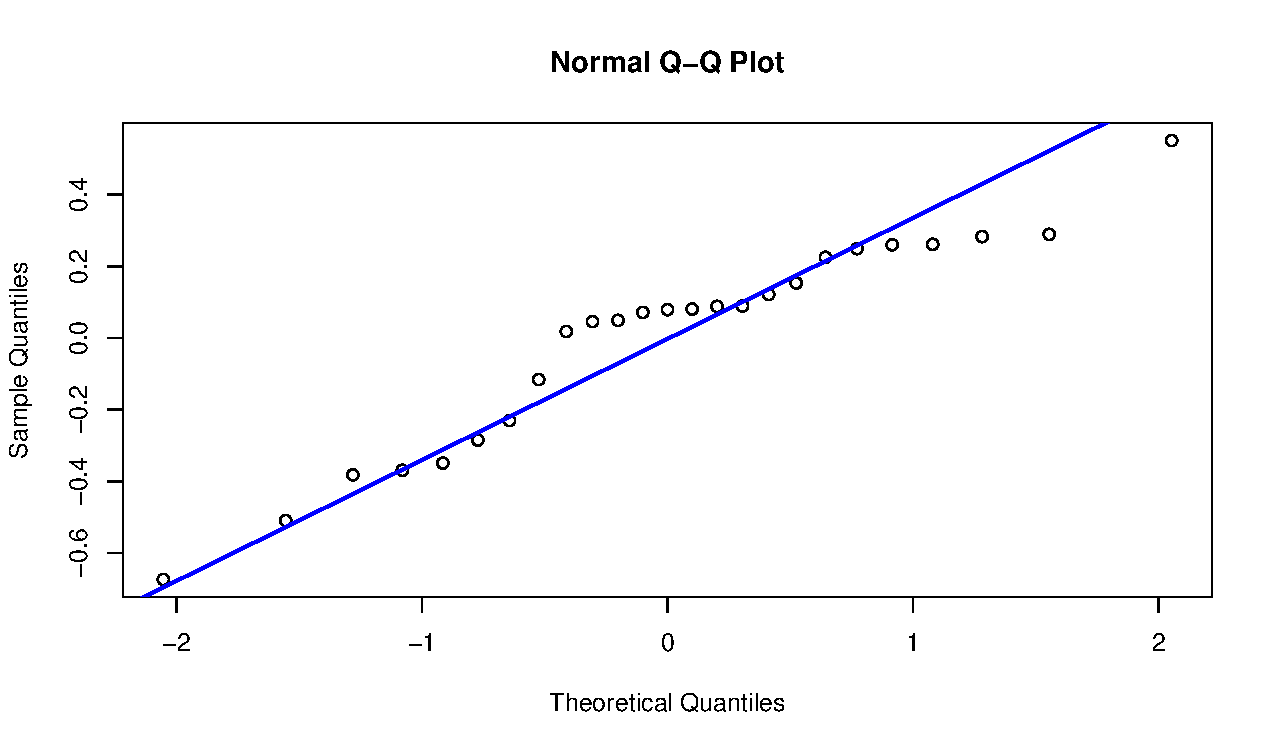
\includegraphics[width=\maxwidth]{figure/unnamed-chunk-55-8} 

}


\begin{kframe}\begin{alltt}
\hlkwd{plot}\hlstd{(lm.loglog}\hlopt{$}\hlstd{fitted.values,}
      \hlstd{lm.loglog}\hlopt{$}\hlstd{residuals,}
\hlkwc{xlab} \hlstd{=} \hlstr{"Fitted Values"}\hlstd{,}
\hlkwc{ylab} \hlstd{=} \hlstr{"Residuals"}\hlstd{)}
\end{alltt}
\end{kframe}

{\centering 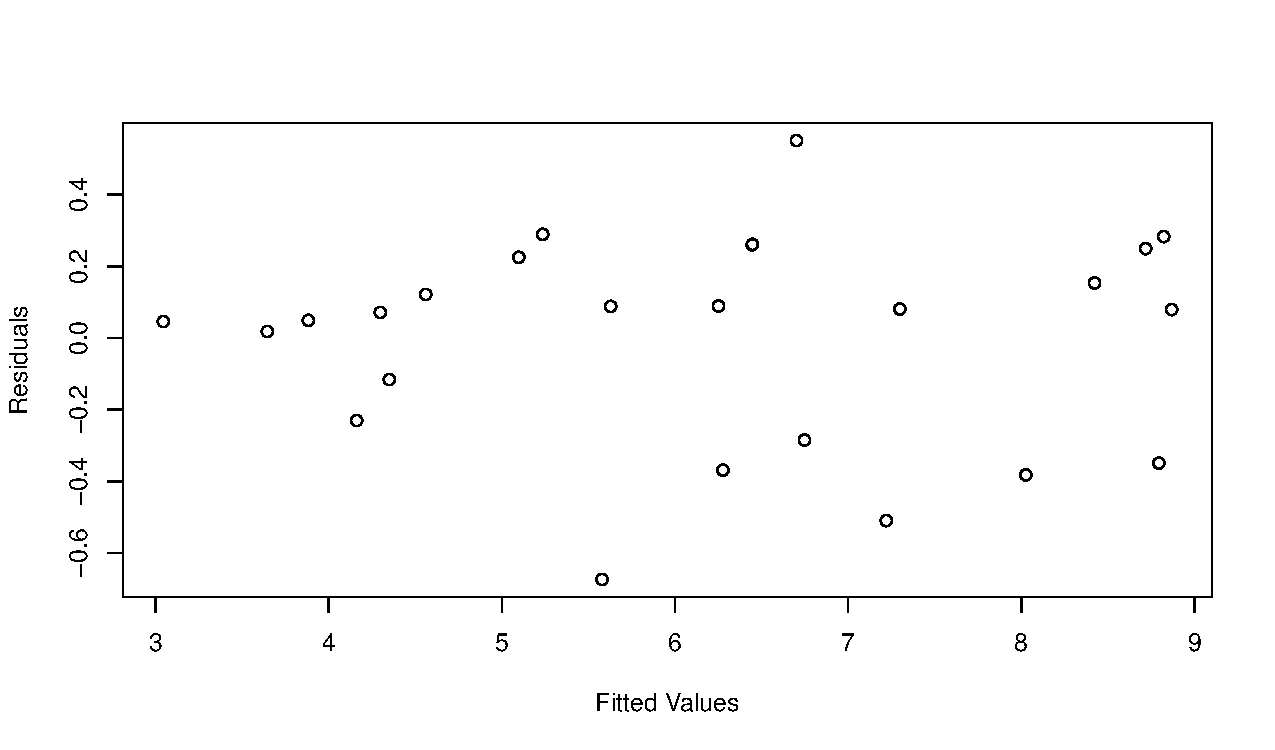
\includegraphics[width=\maxwidth]{figure/unnamed-chunk-55-9} 

}


\begin{kframe}\begin{alltt}
\hlkwd{plot}\hlstd{(}\hlkwd{log}\hlstd{(dat}\hlopt{$}\hlstd{acres),}
      \hlstd{lm.loglog}\hlopt{$}\hlstd{residuals,}
\hlkwc{xlab} \hlstd{=} \hlstr{"Fitted Values"}\hlstd{,}
\hlkwc{ylab} \hlstd{=} \hlstr{"Residuals"}\hlstd{)}
\end{alltt}
\end{kframe}

{\centering 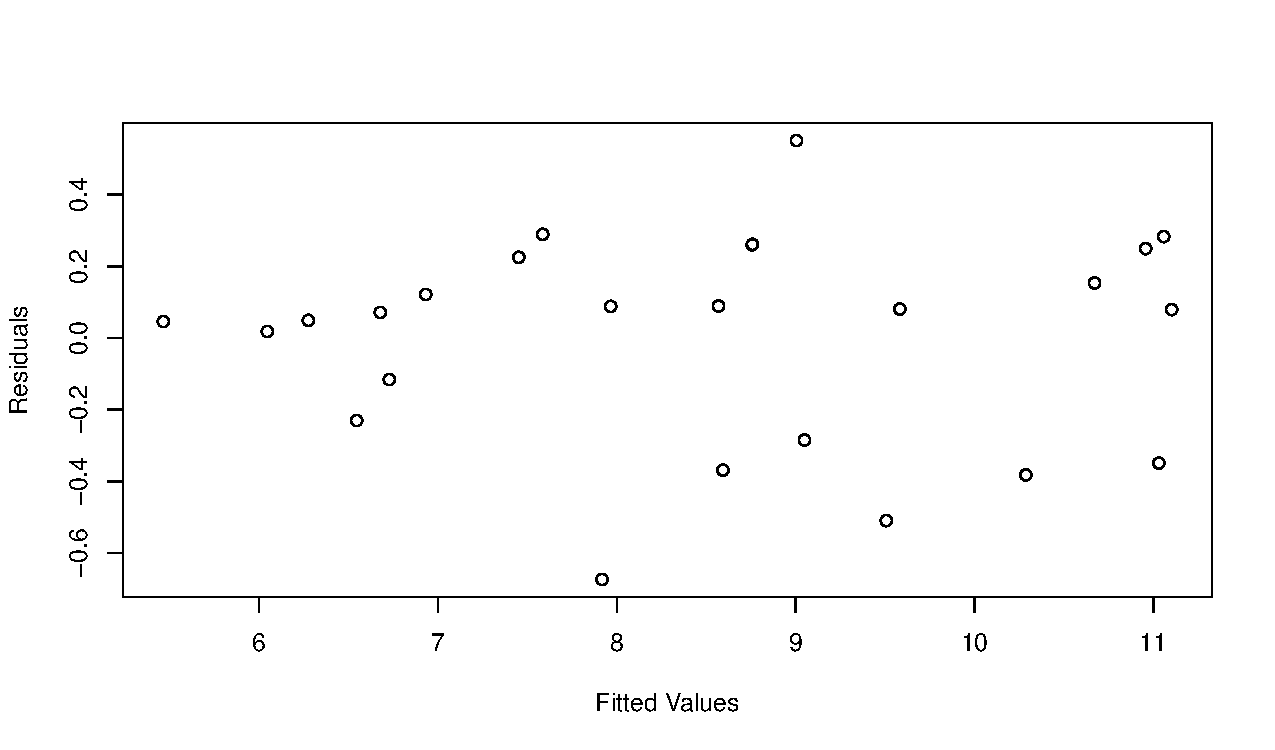
\includegraphics[width=\maxwidth]{figure/unnamed-chunk-55-10} 

}


\begin{kframe}\begin{alltt}
\hlcom{## Python data revisited}
\hlstd{python} \hlkwb{<-} \hlkwd{read.csv}\hlstd{(}\hlstr{"csv/FLpython.csv"}\hlstd{)}
\hlstd{python}\hlopt{$}\hlstd{male} \hlkwb{<-} \hlkwd{ifelse}\hlstd{(python}\hlopt{$}\hlstd{sex} \hlopt{==} \hlstr{'M'}\hlstd{,} \hlnum{1}\hlstd{,} \hlnum{0}\hlstd{)} \hlcom{# 1 = M, 0 =F}
\hlstd{mpf2} \hlkwb{<-} \hlkwd{lm}\hlstd{(fat} \hlopt{~} \hlstd{male} \hlopt{+} \hlstd{mass} \hlopt{+} \hlstd{svl,} \hlkwc{data} \hlstd{= python)}
\hlkwd{summary}\hlstd{(mpf2)}
\end{alltt}
\begin{verbatim}
## 
## Call:
## lm(formula = fat ~ male + mass + svl, data = python)
## 
## Residuals:
##      Min       1Q   Median       3Q      Max 
## -2444.44  -137.38    -6.66   109.22  1530.81 
## 
## Coefficients:
##               Estimate Std. Error t value Pr(>|t|)    
## (Intercept)  204.09840  132.30121   1.543   0.1242    
## male        -196.71705   47.16396  -4.171 4.22e-05 ***
## mass           0.11788    0.00524  22.495  < 2e-16 ***
## svl           -1.59841    0.76433  -2.091   0.0375 *  
## ---
## Signif. codes:  0 '***' 0.001 '**' 0.01 '*' 0.05 '.' 0.1 ' ' 1
## 
## Residual standard error: 360.2 on 244 degrees of freedom
## Multiple R-squared:  0.897,	Adjusted R-squared:  0.8957 
## F-statistic: 708.2 on 3 and 244 DF,  p-value: < 2.2e-16
\end{verbatim}
\begin{alltt}
\hlcom{# Residual plot: vs fitted values}
\hlkwd{plot}\hlstd{(mpf2}\hlopt{$}\hlstd{fitted.values,}
      \hlstd{mpf2}\hlopt{$}\hlstd{residuals,}
\hlkwc{xlab} \hlstd{=} \hlstr{"Fitted Values"}\hlstd{,}
\hlkwc{ylab} \hlstd{=} \hlstr{"Residuals"}\hlstd{)}
\end{alltt}
\end{kframe}

{\centering 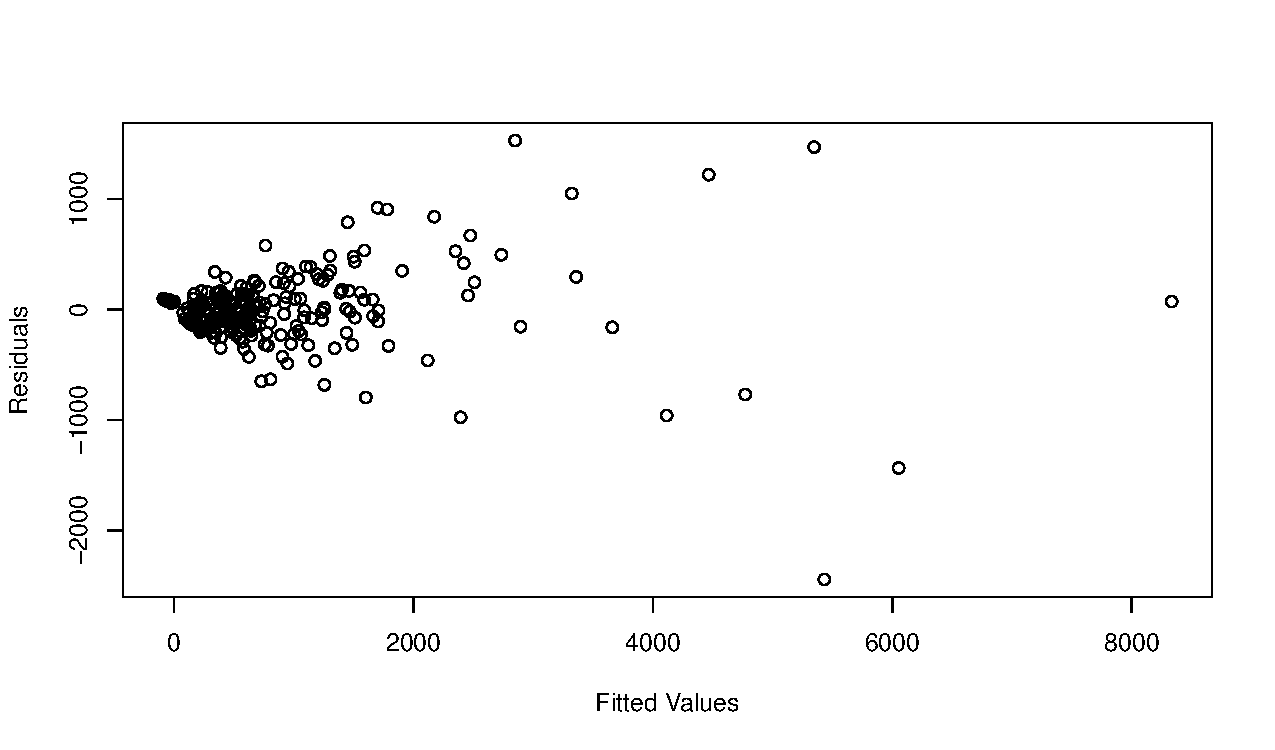
\includegraphics[width=\maxwidth]{figure/unnamed-chunk-55-11} 

}


\begin{kframe}\begin{alltt}
\hlcom{## QQ plot of residuals}
\hlkwd{qqnorm}\hlstd{(mpf2}\hlopt{$}\hlstd{residuals)}
      \hlkwd{qqline}\hlstd{(mpf2}\hlopt{$}\hlstd{residuals,} \hlkwc{col} \hlstd{=} \hlstr{"blue"}\hlstd{,} \hlkwc{lwd} \hlstd{=} \hlnum{2}\hlstd{)}
\end{alltt}
\end{kframe}

{\centering 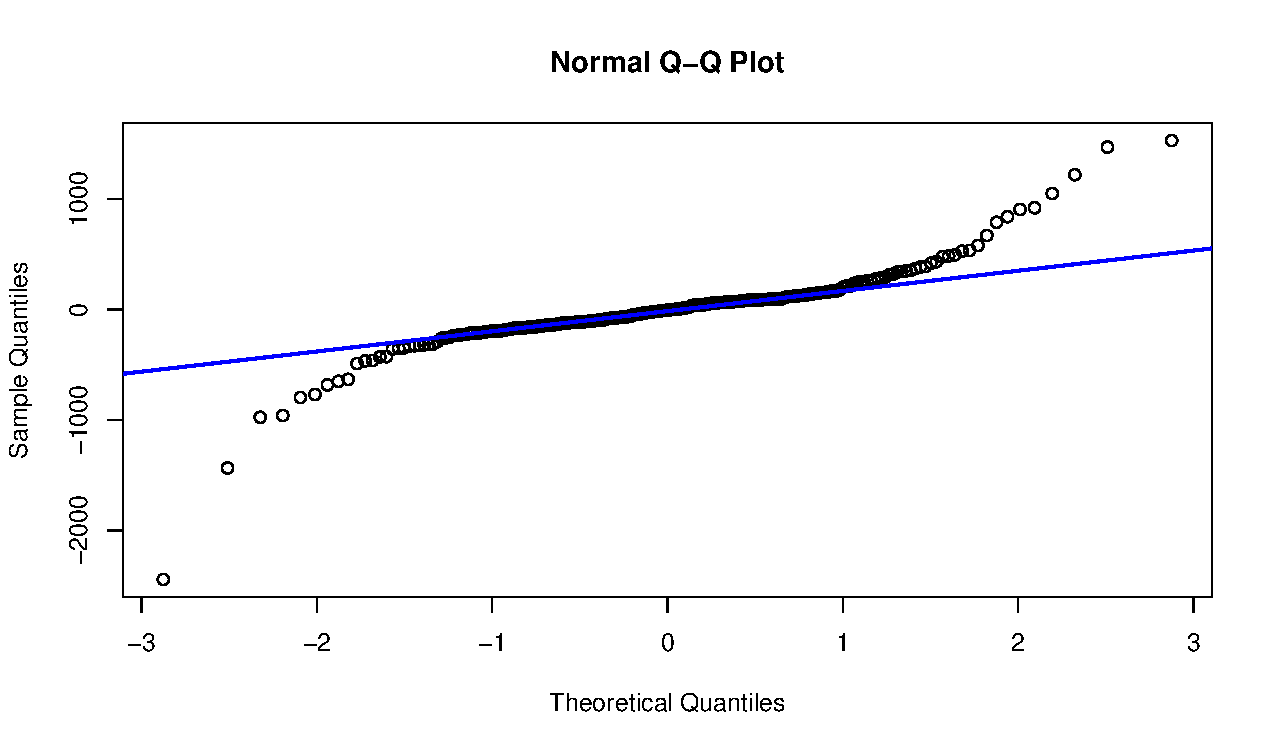
\includegraphics[width=\maxwidth]{figure/unnamed-chunk-55-12} 

}


\begin{kframe}\begin{alltt}
\hlcom{# Try a Box-Cox transformation}
\hlstd{bc} \hlkwb{<-} \hlkwd{boxcox}\hlstd{(mpf2)}
\end{alltt}
\end{kframe}

{\centering 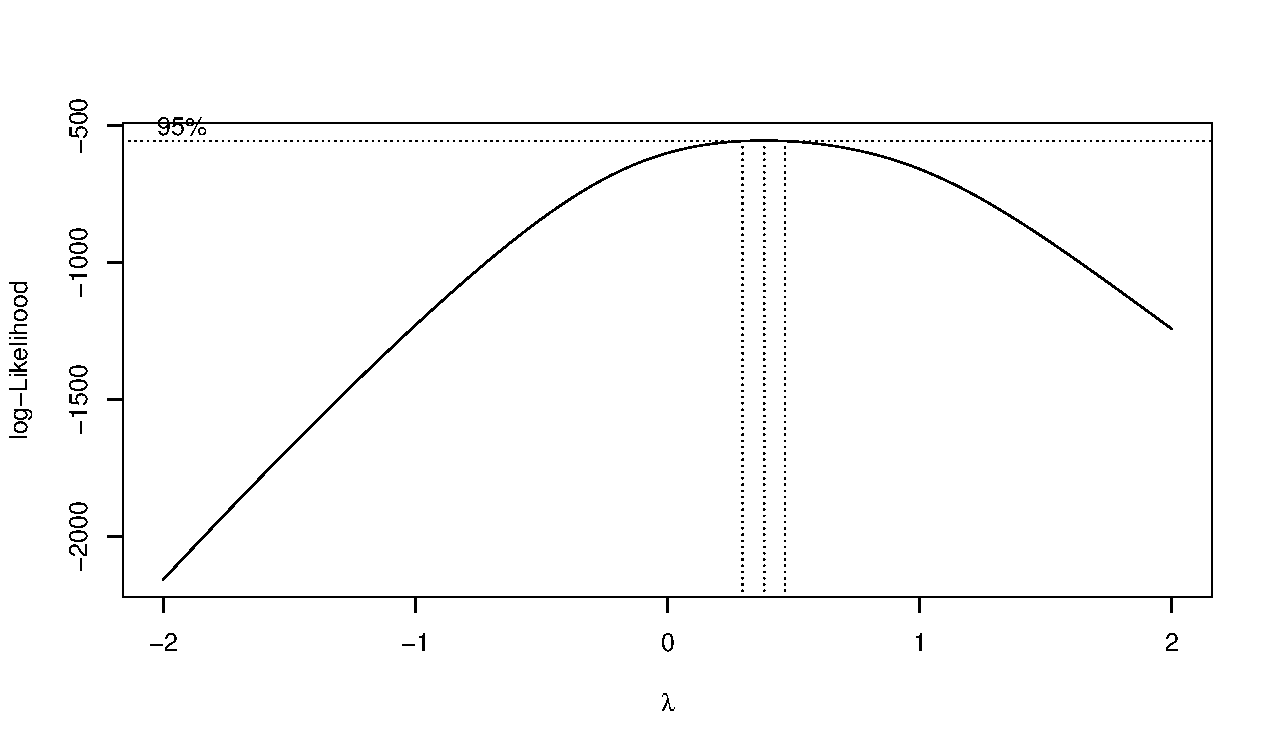
\includegraphics[width=\maxwidth]{figure/unnamed-chunk-55-13} 

}


\begin{kframe}\begin{alltt}
\hlstd{lambda} \hlkwb{<-} \hlstd{bc}\hlopt{$}\hlstd{x[}\hlkwd{which.max}\hlstd{(bc}\hlopt{$}\hlstd{y)]}
      \hlstd{mpf3} \hlkwb{<-} \hlkwd{lm}\hlstd{((fat} \hlopt{^} \hlstd{lambda} \hlopt{-} \hlnum{1}\hlstd{)} \hlopt{/} \hlstd{lambda} \hlopt{~} \hlstd{male} \hlopt{+} \hlstd{mass} \hlopt{+} \hlstd{svl,} \hlkwc{data} \hlstd{= python)}
      \hlkwd{summary}\hlstd{(mpf3)}
\end{alltt}
\begin{verbatim}
## 
## Call:
## lm(formula = (fat^lambda - 1)/lambda ~ male + mass + svl, data = python)
## 
## Residuals:
##     Min      1Q  Median      3Q     Max 
## -19.146  -2.910   0.297   3.688  15.568 
## 
## Coefficients:
##               Estimate Std. Error t value Pr(>|t|)    
## (Intercept) -8.0558134  2.1813183  -3.693 0.000273 ***
## male        -1.7849310  0.7776166  -2.295 0.022560 *  
## mass         0.0004461  0.0000864   5.164 5.03e-07 ***
## svl          0.1431492  0.0126019  11.359  < 2e-16 ***
## ---
## Signif. codes:  0 '***' 0.001 '**' 0.01 '*' 0.05 '.' 0.1 ' ' 1
## 
## Residual standard error: 5.939 on 244 degrees of freedom
## Multiple R-squared:  0.8356,	Adjusted R-squared:  0.8336 
## F-statistic: 413.5 on 3 and 244 DF,  p-value: < 2.2e-16
\end{verbatim}
\begin{alltt}
      \hlkwd{plot}\hlstd{(mpf3}\hlopt{$}\hlstd{fitted.values, mpf3}\hlopt{$}\hlstd{residuals)}
\end{alltt}
\end{kframe}

{\centering 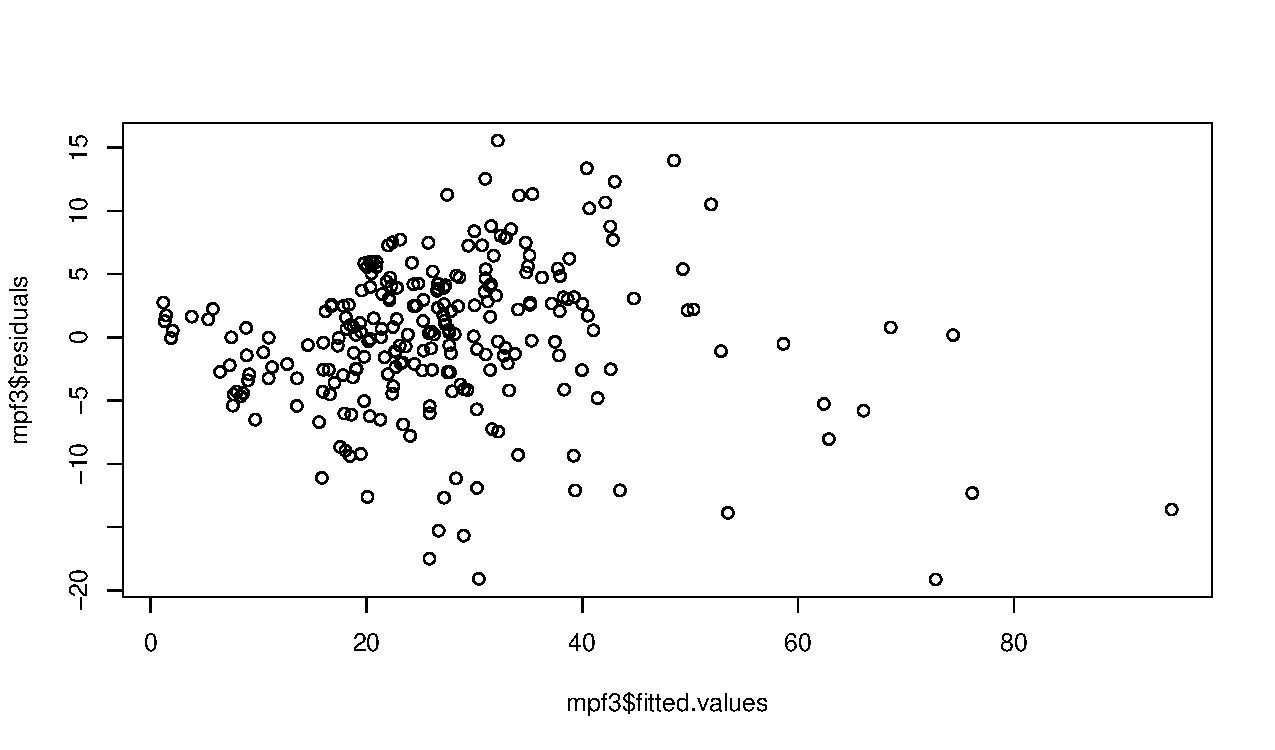
\includegraphics[width=\maxwidth]{figure/unnamed-chunk-55-14} 

}


\begin{kframe}\begin{alltt}
      \hlkwd{plot}\hlstd{(python}\hlopt{$}\hlstd{mass, mpf3}\hlopt{$}\hlstd{residuals)}
\end{alltt}
\end{kframe}

{\centering 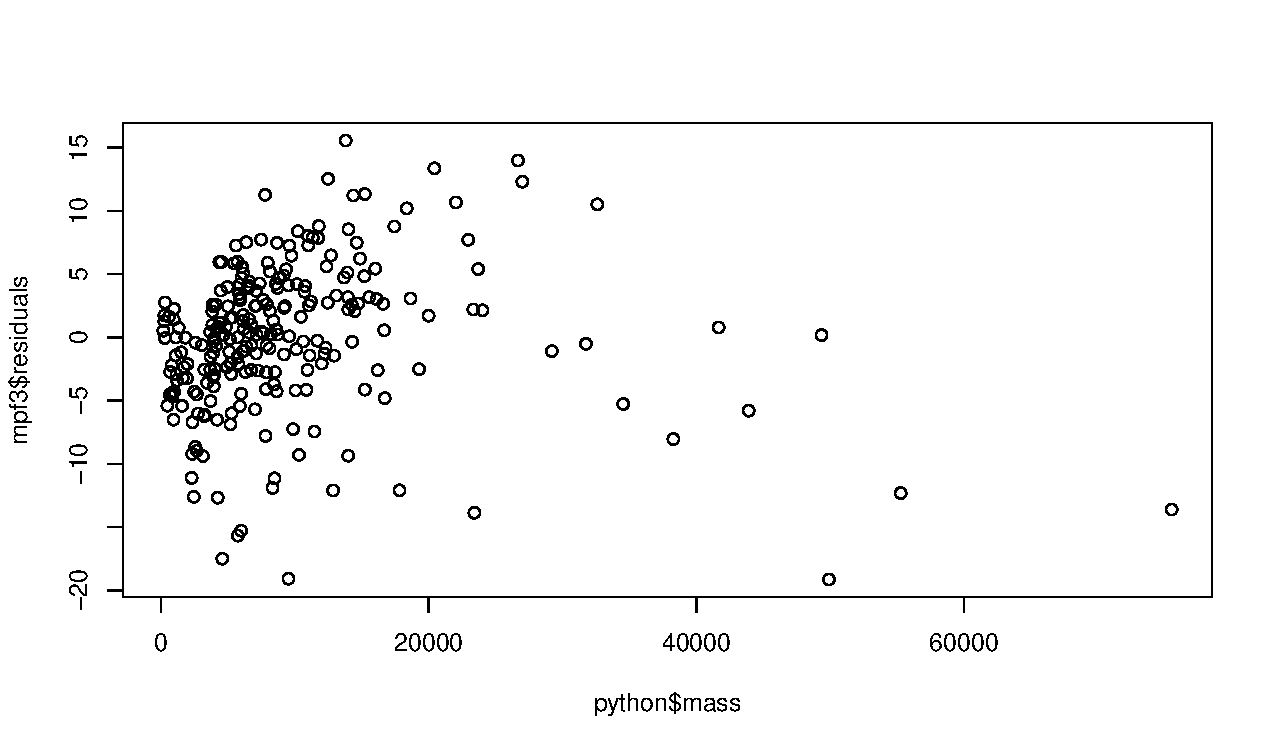
\includegraphics[width=\maxwidth]{figure/unnamed-chunk-55-15} 

}


\begin{kframe}\begin{alltt}
      \hlkwd{plot}\hlstd{(python}\hlopt{$}\hlstd{svl, mpf3}\hlopt{$}\hlstd{residuals)}
\end{alltt}
\end{kframe}

{\centering 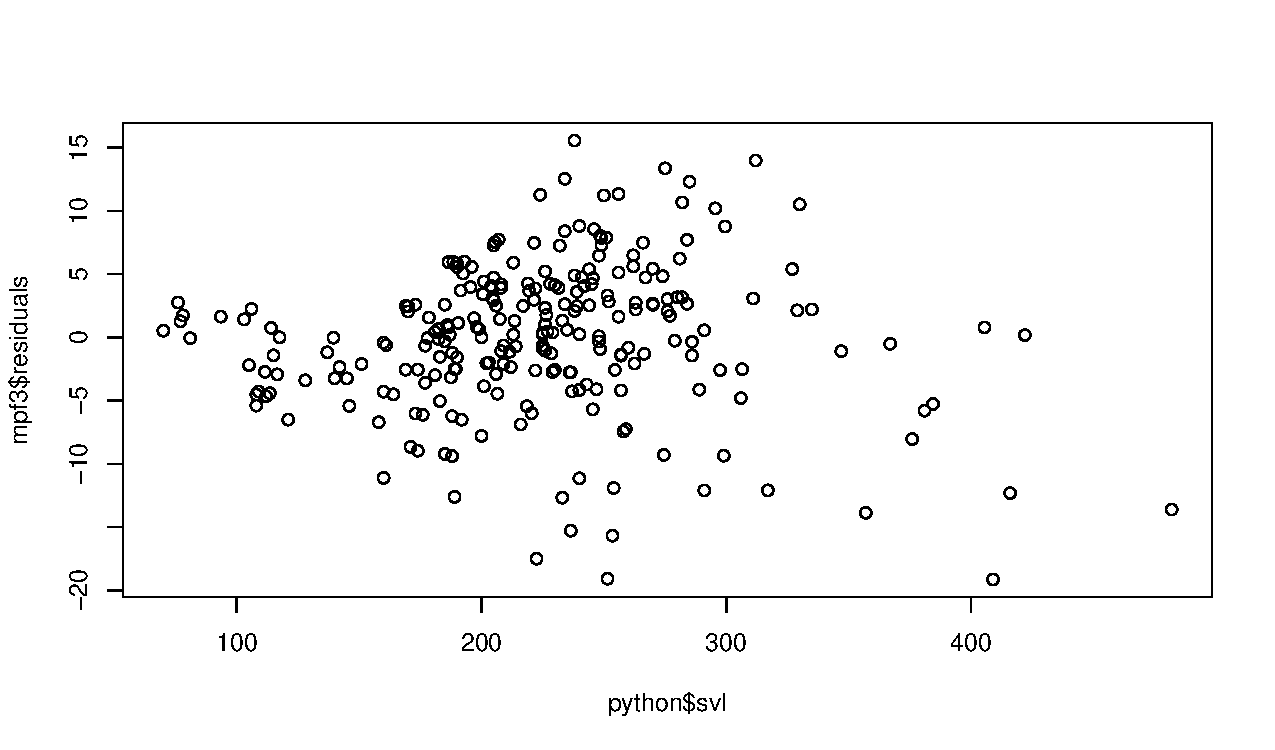
\includegraphics[width=\maxwidth]{figure/unnamed-chunk-55-16} 

}


\begin{kframe}\begin{alltt}
      \hlkwd{qqnorm}\hlstd{(mpf3}\hlopt{$}\hlstd{residuals)}
\hlkwd{qqline}\hlstd{(mpf3}\hlopt{$}\hlstd{residuals,} \hlkwc{col} \hlstd{=} \hlstr{"blue"}\hlstd{,} \hlkwc{lwd} \hlstd{=} \hlnum{2}\hlstd{)}
\end{alltt}
\end{kframe}

{\centering 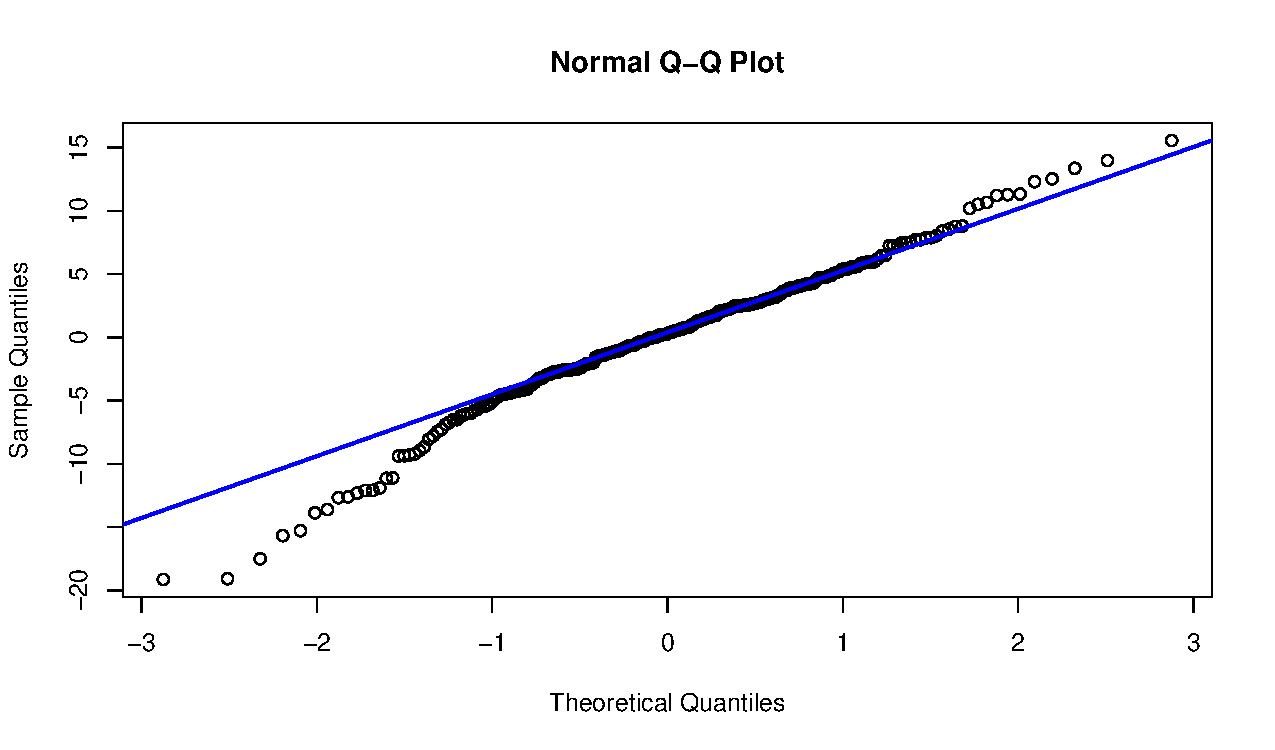
\includegraphics[width=\maxwidth]{figure/unnamed-chunk-55-17} 

}


\begin{kframe}\begin{alltt}
\hlcom{# still some skew, but better!}
\end{alltt}
\end{kframe}
\end{knitrout}
\section{2020-03-10}
\subsection{Templates, STL, Design Patterns}
\begin{lstlisting}
    class Stack {
        int *content;
        int capacity; // capacity of array
        int length; // useful items in array
        public:
            Stack();
            void push(int);
            int top() const; // get the top of the stack
            void pop();
            ~Stack();
    };
\end{lstlisting}
Suppose we wanted a different data type from \code{int}, a \code{string}. One option
would be to manually copy the \code{.cc} and \code{.h} file and replace the types.
A better option, is to use \textbf{C++ Templates}.

\textbf{C++ template class}: a class parameterized on one or more types.
\begin{lstlisting}
    template <typename T> // T is a parameter with a type
    class Stack {
        T *content;
        int capacity; // capacity of array
        int length; // useful items in array
        public:
            Stack();
            void push(T);
            T top() const; // get the top of the stack
            void pop();
            ~Stack();
    };
\end{lstlisting}
There are only minor changes for this simple class.
\begin{lstlisting}
    stack<int> s;
    s.push(s);
    // stack where each entry of the element of the stack is another stack of type string
    stack<stack<string>> bla;
\end{lstlisting}
For the \code{List} class:
\begin{lstlisting}
    template <typename T>
    // not parameterizing the node class
    class List {
        struct Node {
            T data;
            Node *next;
        };
        ...
        public:
            class Iterator {
                Node *curr;
                Iterator(Node *);
                public:
                    T &operator*();
                    Iterator &operator++();
                    bool operator!=(Iterator &);
                    friend class List<T>;
            };
            T ith(int idx);
            void addToFront(T &);
            ~List();
    };
\end{lstlisting}
\begin{lstlisting}
    List<int> l1;
    l1.addToFront(1);
    List<List<int>> l2;
    l2.addToFront(l1);
    // a is a list of ints that are copied by value
    for(auto a : l2) { ... }
    // let's take it by reference
    for (auto &a : l2) {
        for (auto b : a) {
            cout << b;
        }
    }
\end{lstlisting}

\textbf{STL} (Standard Template Library)

\code{std::vector} are dynamic length arrays
\begin{itemize}
    \item automatically resize as needed (possibly even shrink)
\end{itemize}

\begin{lstlisting}
    // Can even be used as a Queue
    #include <vector> // ArrayList from Java
    ...
    vector<int> v; // stack allocated, empty vector
    vector<int> v{3,4}; // [3, 4]
    v.emplace_back(5); // [3, 4, 5] // automatically resizes
    // emplace_back can be more efficient than push_back as it uses move whenever
    // possible; place_back will do a copy
    v.pop_back(); // pop
    v.erase(v.begin()); // vectors have iterators
    v.erase(v.begin() + 3);
    // Suppose we wanted to traverse the vector; there are a lot of options.
    // Option 1
    for (int i = 0; i < v.size(); ++i) {
        cout << v[i]; // overloaded []
    }
    // Option 2
    for (vector<int>::iterator it = v.begin(); it != v.end(); ++it) {
        ...
    }
    // Option 3 (don't need access to the iterator)
    for (auto &i : v) {
        ...
    }
    // Option 4 (reverse iterate), no shortcut based for loop
    // r.begin() (reverse begin)
    // r.end() (reverse end)
    for (vector<int>::reverse.iterator it = v.rbegin(); it != v.rend(); ++it) {
        ...
    }
    // Option 2 and 4 can use auto in the beginning of the for loop
\end{lstlisting}

Code to an interface not to an implementation.
\begin{itemize}
    \item Create abstract classes that define the interface
    \item (Destructor needs \code{virtual} A4Q1), else memory leaks will occur
    \item Work with pointers of this abstract type
          \begin{itemize}
              \item call the interface methods
              \item use \code{virtual} methods where behaviour differs
          \end{itemize}
\end{itemize}

\subsection{Abstract Iterator Design Pattern}
\begin{lstlisting}
    class AbsIter {
        public:
            // need the virtual keyword, else breaks
            virtual int &operator*() const = 0; // pure virtual method
            virtual AbsIter &operator++() = 0;
            virtual bool operator!=(const AbsIter &) = 0;
            virtual ~AbsIter();
    };
\end{lstlisting}

\begin{lstlisting}
    class List {
        ...
        public:
            class Iterator : public AbsIter {
                ...
                public:
                    // override inherited pure virtual methods
            };
    };
\end{lstlisting}

\begin{lstlisting}
    class Set {
        public:
            class Iterator : public AbsIter {
                ...
            };
    };
\end{lstlisting}

\begin{lstlisting}
    void each(AbsIter &start, cons AbsIter &end) {
        while (start != end) {
            // do something with *start
            ++start;
        }
    }
\end{lstlisting}

\begin{lstlisting}
    template <typename Fn>
    // template function
    void foreach(AbsIter &start, const AbsIter &end, Fn f) {
        while (start != end) {
            f(*start); // can only take one parameter (possible to do more)
            ++start;
        }
    }
    void addOne(int &n) { n = n+1; }
    List l;
    // done add to front
    List::Iterator begin = l.begin();
    foreach(begin, l.end(), addOne);
\end{lstlisting}

\makeheading{2019-11-19}
Left class early due to questionable lecturer.


\subsection{R Demo}
\begin{knitrout}
\definecolor{shadecolor}{rgb}{0.969, 0.969, 0.969}\color{fgcolor}\begin{kframe}
\begin{alltt}
\hlcom{## Effect of individual observations}

\hlcom{## Python data revisited}
\hlstd{python} \hlkwb{<-} \hlkwd{read.csv}\hlstd{(}\hlstr{"csv/FLpython.csv"}\hlstd{)}
\hlstd{python}\hlopt{$}\hlstd{male} \hlkwb{<-} \hlkwd{ifelse}\hlstd{(python}\hlopt{$}\hlstd{sex} \hlopt{==} \hlstr{'M'}\hlstd{,} \hlnum{1}\hlstd{,} \hlnum{0}\hlstd{)} \hlcom{# 1 = M, 0 =F}
\hlstd{mpf2} \hlkwb{<-} \hlkwd{lm}\hlstd{(fat} \hlopt{~} \hlstd{male} \hlopt{+} \hlstd{mass} \hlopt{+} \hlstd{svl,} \hlkwc{data} \hlstd{= python)}

\hlcom{# Last time we used a Box-Cox transformation}
\hlkwd{library}\hlstd{(MASS)}
\hlstd{bc} \hlkwb{<-} \hlkwd{boxcox}\hlstd{(mpf2)}
\end{alltt}
\end{kframe}

{\centering 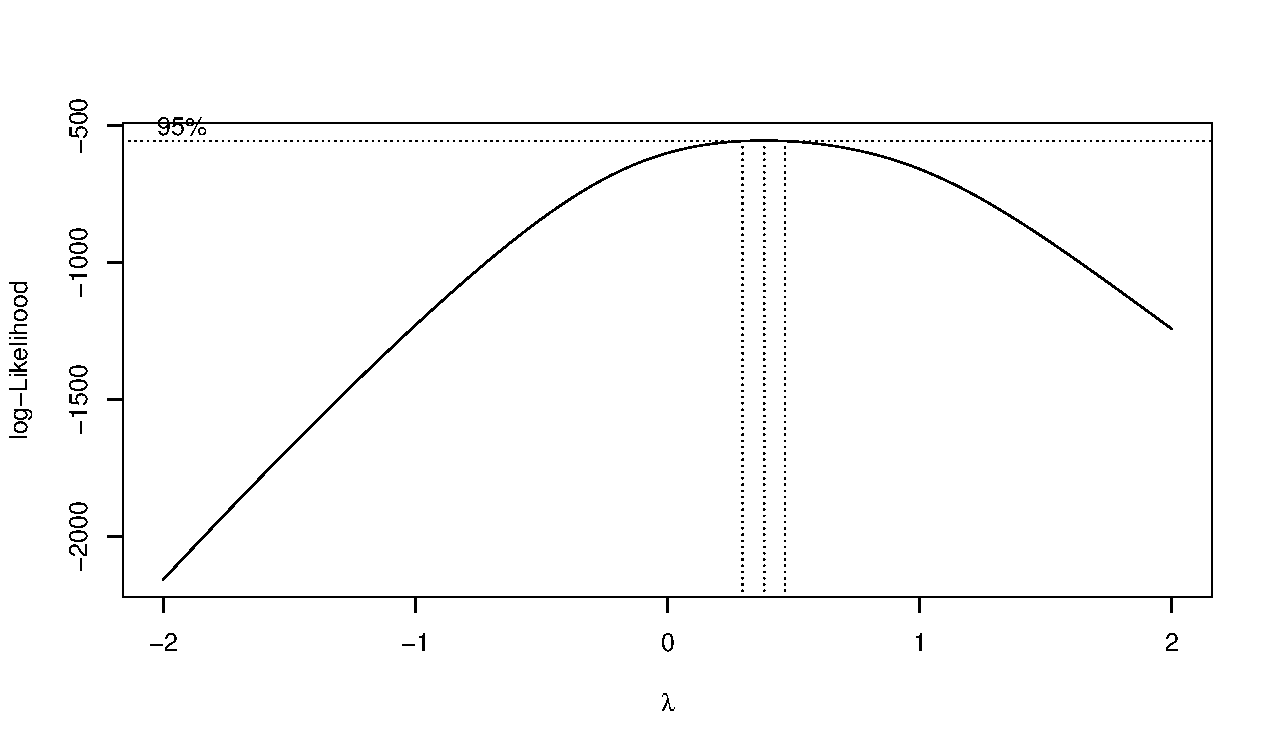
\includegraphics[width=\maxwidth]{figure/unnamed-chunk-56-1} 

}


\begin{kframe}\begin{alltt}
\hlstd{lambda} \hlkwb{<-} \hlstd{bc}\hlopt{$}\hlstd{x[}\hlkwd{which.max}\hlstd{(bc}\hlopt{$}\hlstd{y)]}
      \hlstd{mpf3} \hlkwb{<-} \hlkwd{lm}\hlstd{((fat} \hlopt{^} \hlstd{lambda} \hlopt{-} \hlnum{1}\hlstd{)} \hlopt{/} \hlstd{lambda} \hlopt{~} \hlstd{male} \hlopt{+} \hlstd{mass} \hlopt{+} \hlstd{svl,} \hlkwc{data} \hlstd{= python)}
      \hlkwd{summary}\hlstd{(mpf3)}
\end{alltt}
\begin{verbatim}
## 
## Call:
## lm(formula = (fat^lambda - 1)/lambda ~ male + mass + svl, data = python)
## 
## Residuals:
##     Min      1Q  Median      3Q     Max 
## -19.146  -2.910   0.297   3.688  15.568 
## 
## Coefficients:
##               Estimate Std. Error t value Pr(>|t|)    
## (Intercept) -8.0558134  2.1813183  -3.693 0.000273 ***
## male        -1.7849310  0.7776166  -2.295 0.022560 *  
## mass         0.0004461  0.0000864   5.164 5.03e-07 ***
## svl          0.1431492  0.0126019  11.359  < 2e-16 ***
## ---
## Signif. codes:  0 '***' 0.001 '**' 0.01 '*' 0.05 '.' 0.1 ' ' 1
## 
## Residual standard error: 5.939 on 244 degrees of freedom
## Multiple R-squared:  0.8356,	Adjusted R-squared:  0.8336 
## F-statistic: 413.5 on 3 and 244 DF,  p-value: < 2.2e-16
\end{verbatim}
\begin{alltt}
      \hlkwd{plot}\hlstd{(mpf3}\hlopt{$}\hlstd{fitted.values, mpf3}\hlopt{$}\hlstd{residuals)}
\end{alltt}
\end{kframe}

{\centering 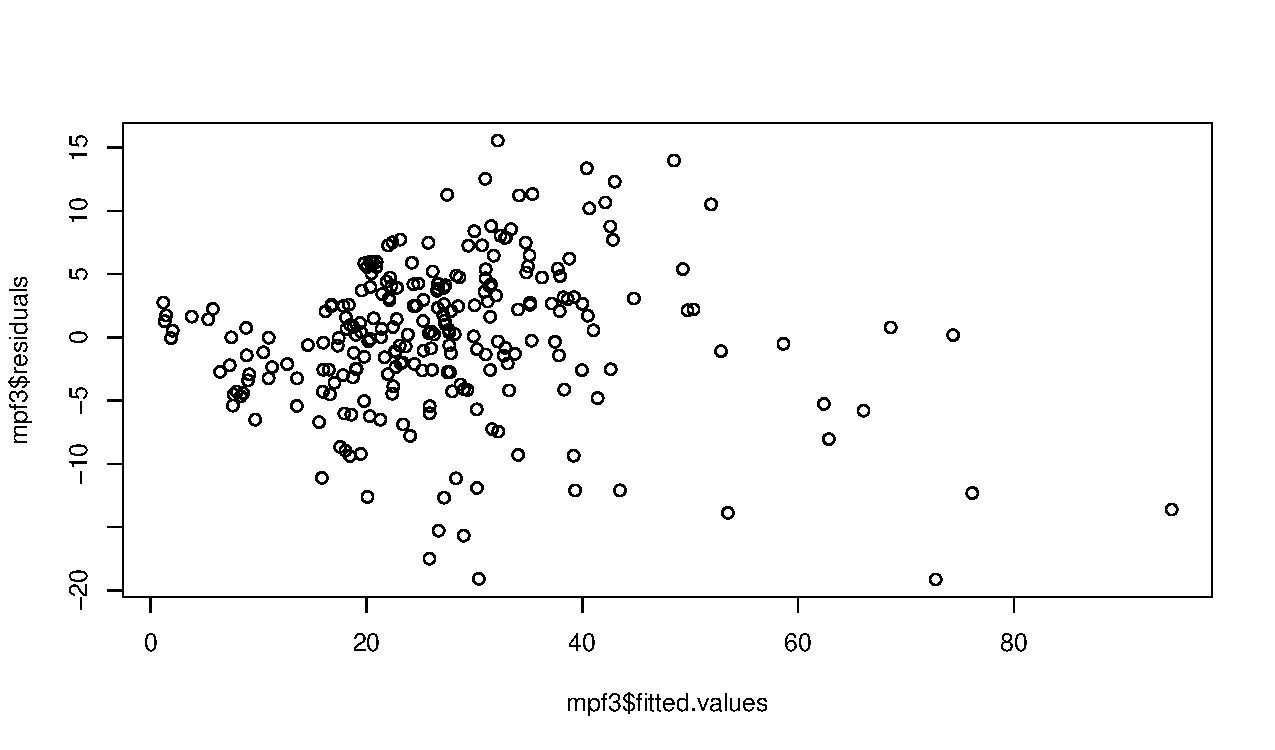
\includegraphics[width=\maxwidth]{figure/unnamed-chunk-56-2} 

}


\begin{kframe}\begin{alltt}
      \hlkwd{qqnorm}\hlstd{(mpf3}\hlopt{$}\hlstd{residuals)}
\hlkwd{qqline}\hlstd{(mpf3}\hlopt{$}\hlstd{residuals,} \hlkwc{col} \hlstd{=} \hlstr{"blue"}\hlstd{,} \hlkwc{lwd} \hlstd{=} \hlnum{2}\hlstd{)}
\end{alltt}
\end{kframe}

{\centering 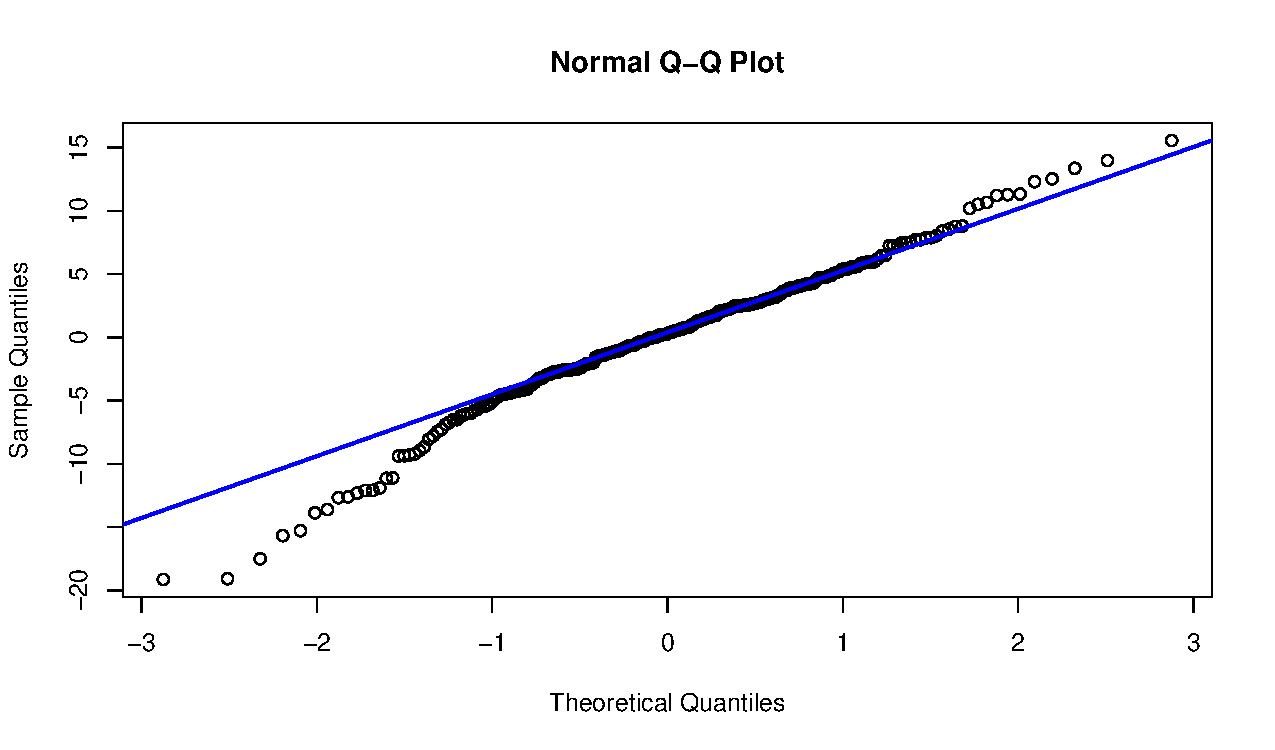
\includegraphics[width=\maxwidth]{figure/unnamed-chunk-56-3} 

}


\end{knitrout}
\begin{knitrout}
\definecolor{shadecolor}{rgb}{0.969, 0.969, 0.969}\color{fgcolor}\begin{kframe}
\begin{alltt}
\hlcom{# Quantities for individual observations}
\hlkwd{studres}\hlstd{(mpf3)}  \hlcom{# studentized residuals}
\hlkwd{hatvalues}\hlstd{(mpf3)} \hlcom{# leverage}
\hlkwd{cooks.distance}\hlstd{(mpf3)} \hlcom{# Cook's distance}
\end{alltt}
\end{kframe}
\end{knitrout}
\begin{knitrout}
\definecolor{shadecolor}{rgb}{0.969, 0.969, 0.969}\color{fgcolor}\begin{kframe}
\begin{alltt}
\hlcom{# Residual plots with studentized residuals}
\hlkwd{plot}\hlstd{(mpf3}\hlopt{$}\hlstd{fitted.values,}
\hlkwd{studres}\hlstd{(mpf3),}
\hlkwc{xlab} \hlstd{=} \hlstr{"Fitted values"}\hlstd{,}
\hlkwc{ylab} \hlstd{=} \hlstr{"Studentized residuals"}\hlstd{)}
\hlkwd{abline}\hlstd{(}\hlkwc{h} \hlstd{=} \hlkwd{c}\hlstd{(}\hlnum{3}\hlstd{,} \hlopt{-}\hlnum{3}\hlstd{),} \hlkwc{col} \hlstd{=} \hlstr{"red"}\hlstd{,} \hlkwc{lty} \hlstd{=} \hlnum{2}\hlstd{)}
\end{alltt}
\end{kframe}

{\centering 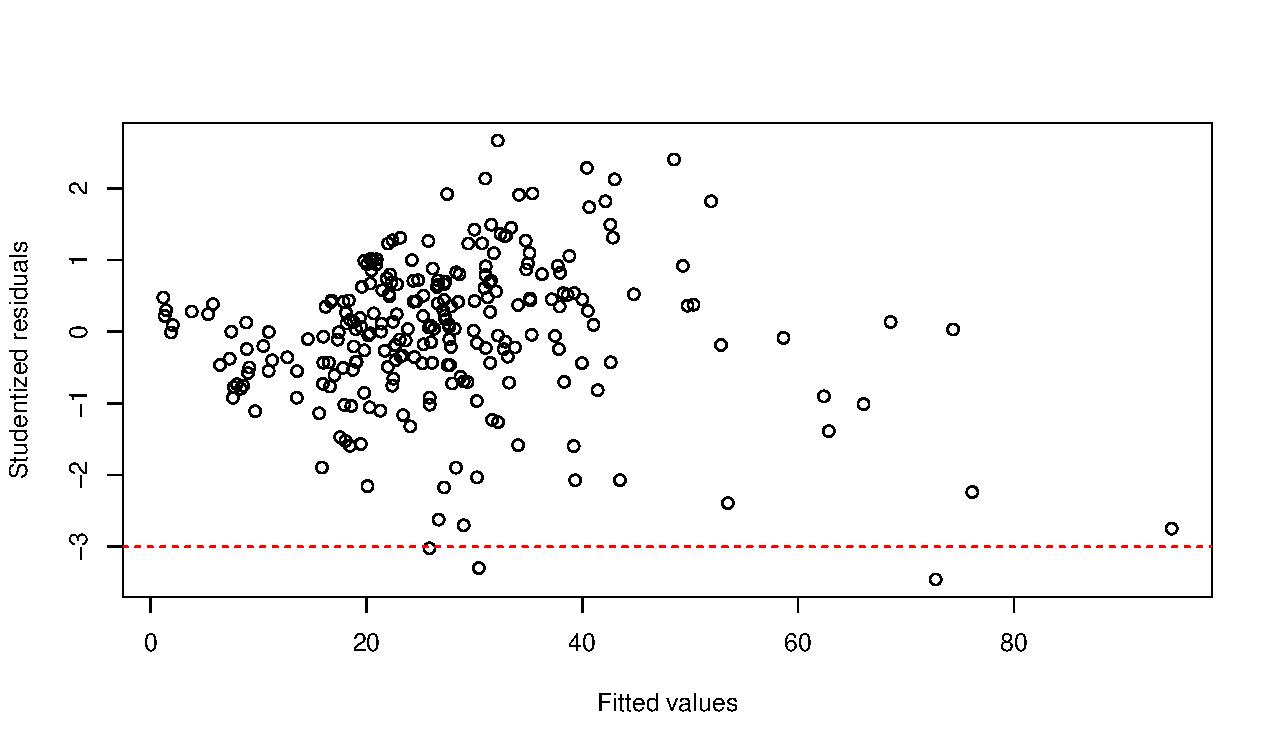
\includegraphics[width=\maxwidth]{figure/unnamed-chunk-58-1} 

}


\begin{kframe}\begin{alltt}
\hlkwd{which}\hlstd{(}\hlkwd{abs}\hlstd{(}\hlkwd{studres}\hlstd{(mpf3))} \hlopt{>} \hlnum{3}\hlstd{)}
\end{alltt}
\begin{verbatim}
## 122 181 245 
## 122 181 245
\end{verbatim}
\begin{alltt}
\hlkwd{qqnorm}\hlstd{(}\hlkwd{studres}\hlstd{(mpf3))}
\hlkwd{qqline}\hlstd{(}\hlkwd{studres}\hlstd{(mpf3),} \hlkwc{col} \hlstd{=} \hlstr{"blue"}\hlstd{,} \hlkwc{lwd} \hlstd{=} \hlnum{2}\hlstd{)}
\end{alltt}
\end{kframe}

{\centering 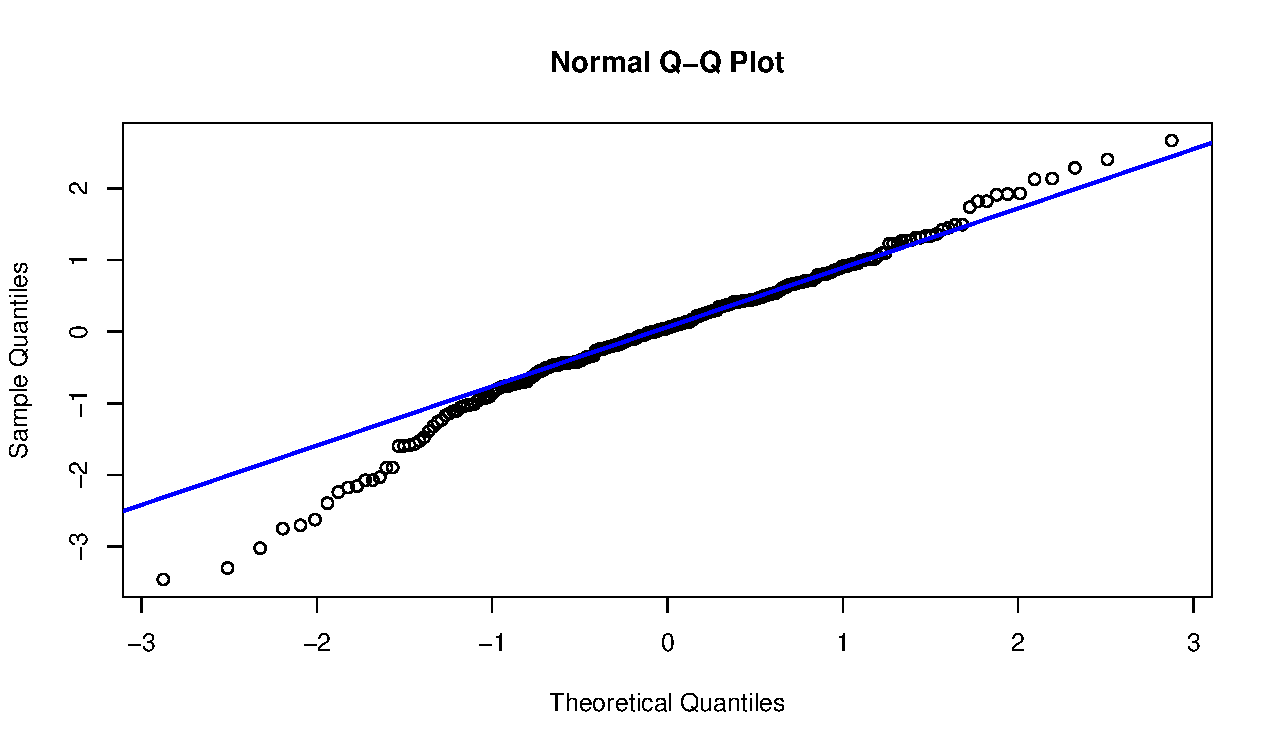
\includegraphics[width=\maxwidth]{figure/unnamed-chunk-58-2} 

}


\begin{kframe}\begin{alltt}
\hlcom{# Leverage}
\hlkwd{plot}\hlstd{(}\hlkwd{hatvalues}\hlstd{(mpf3),} \hlkwc{ylab} \hlstd{=} \hlstr{"Leverage"}\hlstd{)}
\hlkwd{abline}\hlstd{(}\hlkwc{h} \hlstd{=} \hlnum{2} \hlopt{*} \hlkwd{mean}\hlstd{(}\hlkwd{hatvalues}\hlstd{(mpf3)),}
\hlkwc{col} \hlstd{=} \hlstr{"red"}\hlstd{,}
\hlkwc{lty} \hlstd{=} \hlnum{2}\hlstd{)}
\end{alltt}
\end{kframe}

{\centering 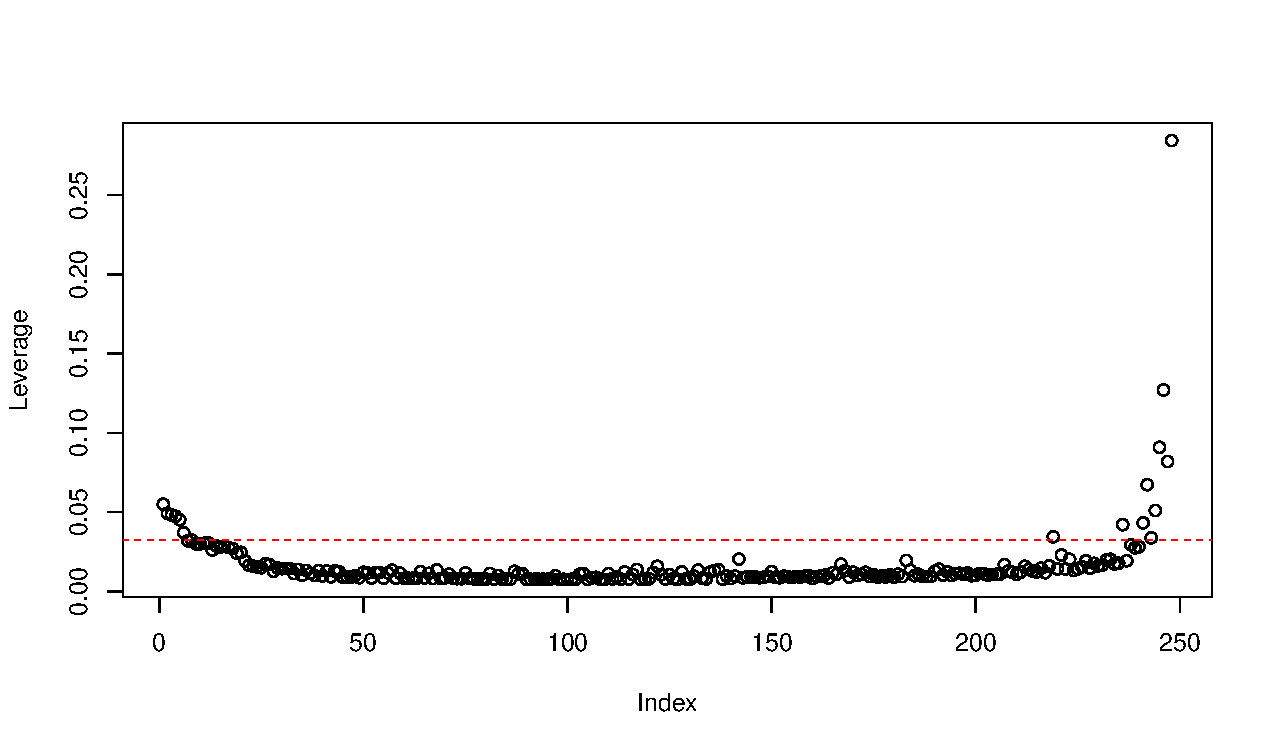
\includegraphics[width=\maxwidth]{figure/unnamed-chunk-58-3} 

}


\begin{kframe}\begin{alltt}
\hlkwd{which}\hlstd{(}\hlkwd{hatvalues}\hlstd{(mpf3)} \hlopt{>} \hlnum{2} \hlopt{*} \hlkwd{mean}\hlstd{(}\hlkwd{hatvalues}\hlstd{(mpf3)))}
\end{alltt}
\begin{verbatim}
##   1   2   3   4   5   6   8 219 236 241 242 243 244 245 246 247 248 
##   1   2   3   4   5   6   8 219 236 241 242 243 244 245 246 247 248
\end{verbatim}
\begin{alltt}
\hlstd{python[}\hlkwd{which}\hlstd{(}\hlkwd{hatvalues}\hlstd{(mpf3)} \hlopt{>} \hlnum{2} \hlopt{*} \hlkwd{mean}\hlstd{(}\hlkwd{hatvalues}\hlstd{(mpf3))), ]}
\end{alltt}
\begin{verbatim}
##     sex   svl  mass length      fat male
## 1     F  70.0   186   77.5    6.000    0
## 2     M  76.0   310   83.8   11.000    1
## 3     M  77.0   260   86.1    6.000    1
## 4     M  78.0   262   87.1    8.000    1
## 5     M  81.0   306   91.1    4.000    1
## 6     M  93.5   605  104.6   18.959    1
## 8     F 105.0   800  117.5   17.000    0
## 219   M 285.0 27000  316.2 3230.000    1
## 236   M 330.0 32600  370.9 4374.000    1
## 241   F 376.0 38280  424.2 3156.000    0
## 242   F 381.0 43910  424.9 4002.000    0
## 243   F 384.5 34540  432.4 3500.000    0
## 244   F 405.5 41660  455.3 5688.000    0
## 245   F 409.0 49900  460.2 2988.000    0
## 246   F 416.0 55260  469.1 4618.000    0
## 247   F 422.0 49350  473.4 6818.000    0
## 248   F 482.0 75500  545.0 8406.000    0
\end{verbatim}
\begin{alltt}
\hlcom{# Cook's distance}
\hlkwd{plot}\hlstd{(}\hlkwd{cooks.distance}\hlstd{(mpf3),} \hlkwc{ylab} \hlstd{=} \hlstr{"Cook's distance"}\hlstd{)}
\hlkwd{abline}\hlstd{(}\hlkwc{h} \hlstd{=} \hlnum{0.5}\hlstd{,} \hlkwc{col} \hlstd{=} \hlstr{"red"}\hlstd{,} \hlkwc{lty} \hlstd{=} \hlnum{2}\hlstd{)}
\end{alltt}
\end{kframe}

{\centering 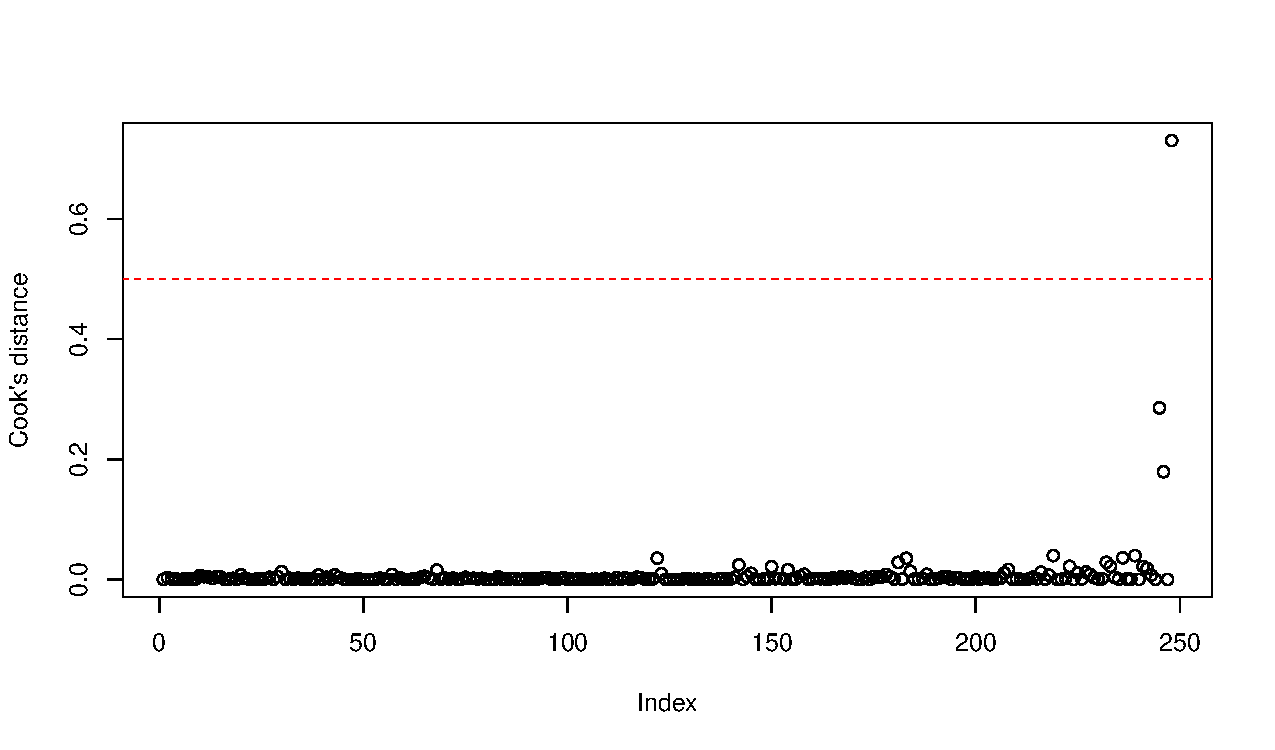
\includegraphics[width=\maxwidth]{figure/unnamed-chunk-58-4} 

}


\begin{kframe}\begin{alltt}
\hlkwd{which}\hlstd{(}\hlkwd{cooks.distance}\hlstd{(mpf3)} \hlopt{>} \hlnum{0.5}\hlstd{)}
\end{alltt}
\begin{verbatim}
## 248 
## 248
\end{verbatim}
\begin{alltt}
\hlcom{# Let's look at actual changes in beta estimates}
\hlstd{mpf3}\hlopt{$}\hlstd{coefficients} \hlcom{# with all the data}
\end{alltt}
\begin{verbatim}
##   (Intercept)          male          mass           svl 
## -8.0558134354 -1.7849310101  0.0004461197  0.1431491887
\end{verbatim}
\begin{alltt}
\hlcom{# e.g., fit without obs 248}
\hlstd{mpf4} \hlkwb{<-}
\hlkwd{lm}\hlstd{((fat} \hlopt{^} \hlstd{lambda} \hlopt{-} \hlnum{1}\hlstd{)} \hlopt{/} \hlstd{lambda} \hlopt{~} \hlstd{male} \hlopt{+} \hlstd{mass} \hlopt{+} \hlstd{svl,} \hlkwc{data} \hlstd{= python[}\hlopt{-}\hlnum{248}\hlstd{, ])}
\hlstd{mpf4}\hlopt{$}\hlstd{coefficients}
\end{alltt}
\begin{verbatim}
##   (Intercept)          male          mass           svl 
## -6.6475616056 -1.6605858218  0.0005743312  0.1313793189
\end{verbatim}
\begin{alltt}
\hlcom{# e.g., fit without obs 50}
\hlstd{mpf5} \hlkwb{<-}
\hlkwd{lm}\hlstd{((fat} \hlopt{^} \hlstd{lambda} \hlopt{-} \hlnum{1}\hlstd{)} \hlopt{/} \hlstd{lambda} \hlopt{~} \hlstd{male} \hlopt{+} \hlstd{mass} \hlopt{+} \hlstd{svl,} \hlkwc{data} \hlstd{= python[}\hlopt{-}\hlnum{50}\hlstd{, ])}
\hlstd{mpf5}\hlopt{$}\hlstd{coefficients}
\end{alltt}
\begin{verbatim}
##   (Intercept)          male          mass           svl 
## -8.0628754675 -1.7805093651  0.0004462354  0.1431573753
\end{verbatim}
\end{kframe}
\end{knitrout}
\makeheading{Lecture 19 | 2020-11-16}
\underline{Prediction Error}
Sometimes a key application of a fitted model
is to do \underline{prediction} on new data
(and is more important than interpretability).

Previously, we saw model selection criteria
that are computed on fitted models
(AIC, BIC, Adjusted $ R^2 $) which assess how
well the model explains the explanatory
power of a model on the \emph{data used to fit the model}
(or \emph{train}).

While these criteria incorporate penalty terms to try
to prevent overfitting, they don't directly assess
how well a model would perform in predicting the response
on new data given predictors.

We mentioned metrics such as MSPE as measures of predictive
accuracy.

To assess accuracy in prediction, we need metrics for
measuring prediction error, e.g.\ evaluated
over $ m $ observations.

\begin{itemize}
    \item Mean-squared error (MSE): If we have $ m $
          observations,
          \[ \text{MSE}=\frac{1}{m} \sum_{i=1}^{m} (y_i-\hat{y}_i)^2 \]
          where $ y_i $ is the actual value, $ \hat{y}_i $ is the
          predicted value (or equivalently, if we apply MSE on the fitted
          data, this would be the fitted value, $ \hat{\mu}_i $;
          if calculated on training data).
          Measured on the scale of $ \sigma^2 $.

          \underline{Note}: MSE is equivalently called MSPE
          if applied on new data.
    \item Root-mean-squared error (RMSE): Square root
          of MSE.\ Measured on the scale of $ \sigma $.
          \[ \text{RSME}=\sqrt{\text{MSE}} \]
    \item Mean absolute error (MAE):
          \[ \text{MAE}=\frac{1}{m} \sum_{i=1}^{m} \abs{y_i-\hat{y}_i} \]
\end{itemize}
Ideally, we have lots of data, conceptualize having three parts.
\begin{table}[ht]
    \centering
    \begin{tabularx}{\linewidth}{@{}YYY@{}}
        \toprule
        Train $ (y_1,y_2,\ldots,y_n) $ & Validation $ (y_{n+1},\ldots,y_{n+v}) $ & Test $ (y_{n+v+1},\ldots,y_{n+v+t}) $ \\
        \midrule
        \begin{itemize}
            \item $ n $ observations
            \item Fit models, as many as we want.
        \end{itemize}
                                       &
        \begin{itemize}
            \item $ v $ observations
            \item Estimate prediction error
                  for each fitted model.
        \end{itemize}
                                       &
        \begin{itemize}
            \item $ t $ observations
            \item Used at the very end for final assessment
                  of our selected model.
        \end{itemize}                                                                                        \\
        \bottomrule
    \end{tabularx}
\end{table}
We have access to train and validation. Test data is from the future,
we won't have access to this until the data is released (say
the actual stock prices were released); that is, assume we don't get
to see this.

For example, using MSE as a metric, based on a fitted model we can
compute
\begin{table}[ht]
    \centering
    \begin{tabularx}{\linewidth}{@{}YYY@{}}
        \toprule
        MSE Train & MSE Validation & MSE Test \\
        \midrule
        \[ \frac{1}{n} \sum_{i=1}^{n} (y_i-\hat{y}_i)^2 \]
                  &
        \[ \frac{1}{m} \sum_{i=n+1}^{n+v} (y_i-\hat{y_i})^2 \]
                  &
        \[ \frac{1}{t} \sum_{i=n+v+1}^{n+v+t}(y_i-\hat{y}_i)^2  \]
        \\
        \bottomrule
    \end{tabularx}
\end{table}

\begin{itemize}
    \item Observe ``MSE Train'' is equal to $ \displaystyle \frac{\SS{Res}}{n} $
          and our usual estimate of $ \hat{\sigma}^2 $
          is a scaled version of this quantity
          to compensate for the number of predictors. Specifically,
          $ \displaystyle  \hat{\sigma}^2=\frac{\SS{Res}}{n-p-1} $
          so it's unbiased.
    \item Consider ``MSE Validation'' as an \emph{estimate} of MSPE
          on new data.
    \item ``MSE Test'' is the actual test of prediction,
          we call this the \emph{actual} MSPE.\
\end{itemize}
\underline{Idea}: We hope that ``MSE Validation'' $ \approx $
``MSE Test'' since neither sets were used to fit the model.

\begin{minipage}{0.7\textwidth}
    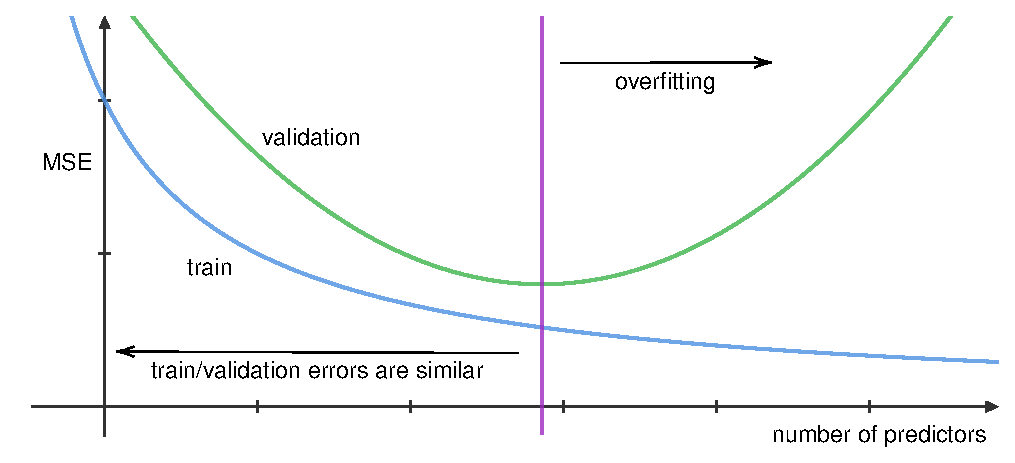
\includegraphics[width=\linewidth]{error.pdf}
\end{minipage}
\begin{minipage}{0.23\textwidth}
    \raggedright{}
    So, if we're using MSE/RMSE
    as a metric (as related to $ \hat{\sigma}^2 $ /$ \hat{\sigma} $)
    and the MSE/RMSE is significantly larger
    on validation compared to train,
    then we probably overfitted the model;
    that is, we can't expect the model
    to generalize well to new data.
\end{minipage}
\section{Cross-Validation}
How to use framework in practice:
\begin{itemize}
    \item Simplest: randomly divide available data
          between train/validation, say $ 80\% $/$ 20\% $ split.

          Weakness:
          \begin{enumerate}
              \item Don't use all data for training.
              \item Only get one estimate of prediction error.
          \end{enumerate}
    \item Better: Use cross-validation scheme (CV). How to
          do CV with $ K $ folds:
          \begin{figure}[!ht]
              \centering
              \begin{tikzpicture}[x=0.75pt,y=0.75pt,yscale=-1,xscale=1]
                  \draw (10,30) -- (270,30) -- (270,50) -- (10,50) -- cycle ;
                  \draw (10,60) -- (270,60) -- (270,80) -- (10,80) -- cycle ;
                  \draw (10,120) -- (270,120) -- (270,140) -- (10,140) -- cycle ;
                  \draw (140,100) node {$\vdots $};
                  \draw (290,40) node {$1$};
                  \draw (290,70) node {$2$};
                  \draw (290,100) node {$\vdots $};
                  \draw (290,130) node {$K$};

                  \draw (45,20) node {$y$};
                  \draw (90,20) node {$x_{1}$};
                  \draw (135,20) node {$x_{2}$};
                  \draw (180,20) node {$\cdots $};
                  \draw (225,20) node {$x_{p}$};
                  \draw (290,18) node {Folds};
              \end{tikzpicture}
          \end{figure}
          \begin{itemize}
              \item Divide available data for train and validation
                    into $ K $ roughly equally sized sets (folds),
                    usually randomly.
              \item For CV $ k $, use data in fold $ k $
                    as validation, and train on
                    the rest of data.
              \item Thus, to estimate the prediction error
                    \emph{for a given model}, we fit it $ K $ times, each
                    time treating the data in folds, $ 1,2,\ldots,K $
                    as validation.
                    Therefore, we get $ K $ estimates of prediction error
                    for that particular model.
              \item For example, using RMSE, we get
                    \[ \overline{\text{RSME}}
                        =\text{RMSE}_1,\text{RMSE}_2,\ldots,\text{RSME}_K \]
                    and can take the average
                    \[ \frac{1}{K} \sum_{k=1}^{K}\text{RSME}_k \]
                    as an estimate for RMSPE on new data (test set).
          \end{itemize}
\end{itemize}


\subsection{R Demo}
\begin{knitrout}
\definecolor{shadecolor}{rgb}{0.969, 0.969, 0.969}\color{fgcolor}\begin{kframe}
\begin{alltt}
\hlcom{## Cross-validation}

\hlcom{## Coffee example  (Coffee Quality Institute, 2018) continued}
\hlstd{coffee} \hlkwb{<-} \hlkwd{read.csv}\hlstd{(}\hlstr{"csv/coffee_arabica.csv"}\hlstd{)}
\hlcom{# 1 = wet, 0 otherwise}
\hlstd{coffee}\hlopt{$}\hlstd{wet} \hlkwb{<-}
      \hlkwd{ifelse}\hlstd{(coffee}\hlopt{$}\hlstd{Processing.Method} \hlopt{==} \hlstr{'Washed / Wet'}\hlstd{,} \hlnum{1}\hlstd{,} \hlnum{0}\hlstd{)}
\hlcom{# 1 = semi/dry, 0 otherwise}
\hlstd{coffee}\hlopt{$}\hlstd{semi} \hlkwb{<-}
      \hlkwd{ifelse}\hlstd{(coffee}\hlopt{$}\hlstd{Processing.Method} \hlopt{==} \hlstr{'Semi-washed / Semi-pulped'}\hlstd{,} \hlnum{1}\hlstd{,} \hlnum{0}\hlstd{)}
\hlstd{coffee}\hlopt{$}\hlstd{Processing.Method} \hlkwb{<-} \hlkwa{NULL}

      \hlstd{N} \hlkwb{<-} \hlkwd{nrow}\hlstd{(coffee)}

      \hlcom{## Train and validation set split}
      \hlkwd{set.seed}\hlstd{(}\hlnum{12345678}\hlstd{)}
      \hlstd{trainInd} \hlkwb{<-} \hlkwd{sample}\hlstd{(}\hlnum{1}\hlopt{:}\hlstd{N,} \hlkwd{round}\hlstd{(N} \hlopt{*} \hlnum{0.8}\hlstd{),} \hlkwc{replace} \hlstd{= F)}
      \hlstd{trainSet} \hlkwb{<-} \hlstd{coffee[trainInd,]}
      \hlstd{validSet} \hlkwb{<-} \hlstd{coffee[}\hlopt{-}\hlstd{trainInd,]}

      \hlcom{# Calculate RMSE on three models each with different variables included}
      \hlstd{m1} \hlkwb{<-}
      \hlkwd{lm}\hlstd{(Flavor} \hlopt{~} \hlstd{wet} \hlopt{+} \hlstd{semi} \hlopt{+} \hlstd{Aroma} \hlopt{+} \hlstd{Aftertaste} \hlopt{+} \hlstd{Body,} \hlkwc{dat} \hlstd{= trainSet)}
      \hlstd{pred1} \hlkwb{<-} \hlkwd{predict}\hlstd{(m1,} \hlkwc{newdata} \hlstd{= validSet)}
      \hlkwd{sqrt}\hlstd{(}\hlkwd{mean}\hlstd{((validSet}\hlopt{$}\hlstd{Flavor} \hlopt{-} \hlstd{pred1)} \hlopt{^} \hlnum{2}\hlstd{))} \hlcom{# RMSE}
\end{alltt}
\begin{verbatim}
## [1] 0.1577479
\end{verbatim}
\begin{alltt}
\hlkwd{mean}\hlstd{(}\hlkwd{abs}\hlstd{(validSet}\hlopt{$}\hlstd{Flavor} \hlopt{-} \hlstd{pred1))} \hlcom{# MAE}
\end{alltt}
\begin{verbatim}
## [1] 0.113643
\end{verbatim}
\begin{alltt}
      \hlstd{m2} \hlkwb{<-} \hlkwd{lm}\hlstd{(}
      \hlstd{Flavor} \hlopt{~} \hlstd{wet} \hlopt{+} \hlstd{Aroma} \hlopt{+} \hlstd{Aftertaste} \hlopt{+}
      \hlstd{Body} \hlopt{+} \hlstd{Acidity} \hlopt{+} \hlstd{Balance} \hlopt{+} \hlstd{Sweetness} \hlopt{+} \hlstd{Uniformity} \hlopt{+} \hlstd{Moisture,}
      \hlkwc{dat} \hlstd{= trainSet}
      \hlstd{)}
      \hlstd{pred2} \hlkwb{<-} \hlkwd{predict}\hlstd{(m2,} \hlkwc{newdata} \hlstd{= validSet)}
      \hlkwd{sqrt}\hlstd{(}\hlkwd{mean}\hlstd{((validSet}\hlopt{$}\hlstd{Flavor} \hlopt{-} \hlstd{pred2)} \hlopt{^} \hlnum{2}\hlstd{))}
\end{alltt}
\begin{verbatim}
## [1] 0.1426565
\end{verbatim}
\begin{alltt}
\hlstd{m3} \hlkwb{<-} \hlkwd{lm}\hlstd{(Flavor} \hlopt{~} \hlstd{Aroma} \hlopt{+} \hlstd{Aftertaste,} \hlkwc{dat} \hlstd{= trainSet)}
\hlstd{pred3} \hlkwb{<-} \hlkwd{predict}\hlstd{(m3,} \hlkwc{newdata} \hlstd{= validSet)}
\hlkwd{sqrt}\hlstd{(}\hlkwd{mean}\hlstd{((validSet}\hlopt{$}\hlstd{Flavor} \hlopt{-} \hlstd{pred3)} \hlopt{^} \hlnum{2}\hlstd{))}
\end{alltt}
\begin{verbatim}
## [1] 0.1615385
\end{verbatim}
\begin{alltt}
\hlcom{# K fold cross validation}
\hlstd{K} \hlkwb{<-} \hlnum{5}
\hlstd{validSetSplits} \hlkwb{<-} \hlkwd{sample}\hlstd{((}\hlnum{1}\hlopt{:}\hlstd{N)} \hlopt \hlstd{K} \hlopt{+} \hlnum{1}\hlstd{)}
\hlstd{RMSE1} \hlkwb{<-} \hlkwd{c}\hlstd{()}
\hlstd{RMSE2} \hlkwb{<-} \hlkwd{c}\hlstd{()}
\hlstd{RMSE3} \hlkwb{<-} \hlkwd{c}\hlstd{()}
\hlkwa{for} \hlstd{(k} \hlkwa{in} \hlnum{1}\hlopt{:}\hlstd{K) \{}
            \hlstd{validSet} \hlkwb{<-} \hlstd{coffee[validSetSplits} \hlopt{==} \hlstd{k,]}
            \hlstd{trainSet} \hlkwb{<-} \hlstd{coffee[validSetSplits} \hlopt{!=} \hlstd{k,]}

            \hlstd{m1} \hlkwb{<-}
            \hlkwd{lm}\hlstd{(Flavor} \hlopt{~} \hlstd{wet} \hlopt{+} \hlstd{semi} \hlopt{+} \hlstd{Aroma} \hlopt{+} \hlstd{Aftertaste} \hlopt{+} \hlstd{Body,} \hlkwc{dat} \hlstd{= trainSet)}
            \hlstd{pred1} \hlkwb{<-} \hlkwd{predict}\hlstd{(m1,} \hlkwc{newdata} \hlstd{= validSet)}
            \hlstd{RMSE1[k]} \hlkwb{<-} \hlkwd{sqrt}\hlstd{(}\hlkwd{mean}\hlstd{((validSet}\hlopt{$}\hlstd{Flavor} \hlopt{-} \hlstd{pred1)} \hlopt{^} \hlnum{2}\hlstd{))}

                  \hlstd{m2} \hlkwb{<-} \hlkwd{lm}\hlstd{(}
                  \hlstd{Flavor} \hlopt{~} \hlstd{wet} \hlopt{+} \hlstd{Aroma} \hlopt{+} \hlstd{Aftertaste} \hlopt{+}
                  \hlstd{Body} \hlopt{+} \hlstd{Acidity} \hlopt{+} \hlstd{Balance} \hlopt{+} \hlstd{Sweetness} \hlopt{+} \hlstd{Uniformity} \hlopt{+} \hlstd{Moisture,}
                  \hlkwc{dat} \hlstd{= trainSet}
                  \hlstd{)}
                  \hlstd{pred2} \hlkwb{<-} \hlkwd{predict}\hlstd{(m2,} \hlkwc{newdata} \hlstd{= validSet)}
                  \hlstd{RMSE2[k]} \hlkwb{<-} \hlkwd{sqrt}\hlstd{(}\hlkwd{mean}\hlstd{((validSet}\hlopt{$}\hlstd{Flavor} \hlopt{-} \hlstd{pred2)} \hlopt{^} \hlnum{2}\hlstd{))}

            \hlstd{m3} \hlkwb{<-} \hlkwd{lm}\hlstd{(Flavor} \hlopt{~} \hlstd{Aroma} \hlopt{+} \hlstd{Aftertaste,} \hlkwc{dat} \hlstd{= trainSet)}
            \hlstd{pred3} \hlkwb{<-} \hlkwd{predict}\hlstd{(m3,} \hlkwc{newdata} \hlstd{= validSet)}
            \hlstd{RMSE3[k]} \hlkwb{<-} \hlkwd{sqrt}\hlstd{(}\hlkwd{mean}\hlstd{((validSet}\hlopt{$}\hlstd{Flavor} \hlopt{-} \hlstd{pred3)} \hlopt{^} \hlnum{2}\hlstd{))}
      \hlstd{\}}

\hlstd{RMSE1}
\end{alltt}
\begin{verbatim}
## [1] 0.1479415 0.1653329 0.1556385 0.1656876 0.1482716
\end{verbatim}
\begin{alltt}
\hlstd{RMSE2}
\end{alltt}
\begin{verbatim}
## [1] 0.1427025 0.1525461 0.1478815 0.1620440 0.1384244
\end{verbatim}
\begin{alltt}
\hlstd{RMSE3}
\end{alltt}
\begin{verbatim}
## [1] 0.1513836 0.1667202 0.1616626 0.1675113 0.1532496
\end{verbatim}
\begin{alltt}
\hlkwd{mean}\hlstd{(RMSE1)}
\end{alltt}
\begin{verbatim}
## [1] 0.1565744
\end{verbatim}
\begin{alltt}
\hlkwd{mean}\hlstd{(RMSE2)}
\end{alltt}
\begin{verbatim}
## [1] 0.1487197
\end{verbatim}
\begin{alltt}
\hlkwd{mean}\hlstd{(RMSE3)}
\end{alltt}
\begin{verbatim}
## [1] 0.1601055
\end{verbatim}
\end{kframe}
\end{knitrout}
\makeheading{Lecture 20 | 2020-11-18}
\section{Combining Cross Validation With Model Selection}
\begin{itemize}
      \item Given some candidate models (e.g., with different
            variables included) we can do $ K $-fold
            cross-validation using each of them, and choose the one
            with the lowest average prediction error across
            the folds, e.g., $ \displaystyle
                  \frac{1}{K} \sum_{k=1}^{K} \text{RSME}_k $.
      \item How to choose $ K $? Some common choices are:
            \begin{itemize}
                  \item $ K=5 $
                  \item $ K=10 $
                  \item $ K=N $ (number of observations for train/valid).
                        This is commonly known as ``leave one out'' (LOO).
            \end{itemize}
            The more folds, the higher the computational time, but
            it can give a better estimate of prediction error.
      \item What if we are not given a list of models to compare?
            (and if there are too many predictors to do all possible
            regressions). Then, we can combine cross-validation with
            \emph{model selection procedures} (criteria based on training
            data and search strategy).
\end{itemize}
To estimate the prediction error for a given
\emph{model selection procedure} we apply it $ K $ times,
each time treating observations in fold $ 1,2,\ldots,K $
as validation sample, e.g., use the \emph{average}
RMSE and choose the model selection procedure
with the lowest estimated prediction error.

\underline{Note}: actual variables selected in each fold might
be different.

\underline{Recommendation}: apply chosen
model selection \emph{procedure} (lowest estimated prediction error)
to the entire set of observations available for training
and validation to get a final model (for applications
to test data).

Recall we have:
\begin{itemize}
      \item $ \text{AIC}=2q-2\ln[L(\hat{\theta})] $
      \item $ \text{BIC}=q\ln(n)-2\ln[L(\hat{\theta})] $
\end{itemize}
We can go further (and beyond \emph{PLUS ULTRA!}) and consider the following.
\begin{Definition}{$ L_0 $ Penalized Likelihood}{}
      For any $ \lambda>0 $,
      \[ q\lambda -2\ln[L(\hat{\theta})] \]
\end{Definition}
\underline{Beyond Stepwise Regression}
\begin{itemize}
      \item Stepwise is a deterministic algorithm which is fast,
            but might not give optimal model selected.
      \item Could try stochastic algorithm, e.g., iterative
            conditional minimization (ICM)
\end{itemize}

\section{Iterative Conditional Minimization}
Start with a model with just intercept.
For a given random seed, take predictors $ x_1,\ldots,x_p $
and randomly re-order them into $ x_{(1)},\ldots,x_{(p)} $.
For $ j=1,\ldots,p $: (let $ \mathcal{S} $ be the predictors
currently in model, so start at $ \mathcal{S}=\emptyset $).
\begin{itemize}
      \item If $ x_{(j)} $ is not in $ \mathcal{S} $:
            \begin{itemize}
                  \item Fit model with $ \mathcal{S} $.
                        If addition of $ x_{(j)} $ improves criterion,
                        then add $ x_{(j)} $ to $ \mathcal{S} $.
            \end{itemize}
      \item If $ x_{(j)} $ is in $ \mathcal{S} $:
            \begin{itemize}
                  \item Fit model removing $ x_{(j)} $. If excluding
                        $ x_{(j)} $ improves criterion, then remove
                        $ x_{(j)} $ from $ \mathcal{S} $.
            \end{itemize}
\end{itemize}
Repeat for loop until no predictors are added/removed
from an entire pass through the for loop.
\begin{Remark}{}{}
      Different random orderings could give different
      sets $ \mathcal{S} $ at end of procedure, could pick one
      that has the best criterion overall.
\end{Remark}


\subsection{R Demo}
\begin{knitrout}
\definecolor{shadecolor}{rgb}{0.969, 0.969, 0.969}\color{fgcolor}\begin{kframe}
\begin{alltt}
\hlcom{## Cross-validation with model selection}

\hlcom{# Dataset from paper "Where does Haydn end and Mozart begin?}
\hlcom{# Composer classification of string quartets"}
\hlcom{# (Journal of New Music Research, vol 49, 457-476)}
\hlstd{HM} \hlkwb{<-} \hlkwd{read.csv}\hlstd{(}\hlstr{"haydn-mozart.csv"}\hlstd{)}
\hlstd{HM[,}\hlnum{1}\hlstd{]} \hlkwb{<-} \hlkwa{NULL} \hlcom{# first col is just name of quartet, remove it}
\hlkwd{dim}\hlstd{(HM)} \hlcom{# 285 observations, 1116 columns}

\hlcom{# Let's treat "number of notes in violin part" as the response}
\hlcom{# That's variable name "count_pitch_1" and column 683 of data matrix}
\hlcom{# So we have 1115 possible predictors}

\hlcom{# More model selection, for clarity start with one train/validation split}
\hlstd{N} \hlkwb{<-} \hlkwd{nrow}\hlstd{(HM)}
\hlkwd{set.seed}\hlstd{(}\hlnum{12345678}\hlstd{)}
\hlstd{trainInd} \hlkwb{<-} \hlkwd{sample}\hlstd{(}\hlnum{1}\hlopt{:}\hlstd{N,} \hlkwd{round}\hlstd{(N}\hlopt{*}\hlnum{0.8}\hlstd{),} \hlkwc{replace}\hlstd{=F)}
\hlstd{trainSet} \hlkwb{<-} \hlstd{HM[trainInd,]}
\hlstd{validSet} \hlkwb{<-} \hlstd{HM[}\hlopt{-}\hlstd{trainInd,]}

\hlkwd{library}\hlstd{(MASS)}
\hlcom{# Full model and empty model with just intercept}
\hlstd{full} \hlkwb{<-} \hlkwd{lm}\hlstd{(count_pitch_1} \hlopt{~} \hlstd{.,} \hlkwc{data} \hlstd{= trainSet)}
\hlstd{empty} \hlkwb{<-} \hlkwd{lm}\hlstd{(count_pitch_1} \hlopt{~} \hlnum{1}\hlstd{,} \hlkwc{data} \hlstd{=trainSet)}

\hlcom{# Stepwise forward with BIC}
\hlkwd{stepAIC}\hlstd{(}\hlkwc{object} \hlstd{= empty,} \hlkwc{scope} \hlstd{=} \hlkwd{list}\hlstd{(}\hlkwc{upper} \hlstd{= full,} \hlkwc{lower} \hlstd{= empty),} \hlkwc{direction} \hlstd{=} \hlstr{"forward"}\hlstd{,} \hlkwc{k} \hlstd{=} \hlkwd{log}\hlstd{(}\hlkwd{nrow}\hlstd{(trainSet)))}
\hlstd{m1} \hlkwb{<-} \hlkwd{lm}\hlstd{(}\hlkwc{formula} \hlstd{= count_pitch_1} \hlopt{~} \hlstd{Prop_m3_num_0_8.1} \hlopt{+} \hlstd{count_pitch_3} \hlopt{+}
\hlstd{Prop_m3_num_0_8.3} \hlopt{+} \hlstd{Prop_m3_mean_8.1} \hlopt{+} \hlstd{count_pitch_4} \hlopt{+} \hlstd{Dev_count_8_thresh4.393.1} \hlopt{+}
\hlstd{Prop_m3_mean_8.3} \hlopt{+} \hlstd{mean_time_3} \hlopt{+} \hlstd{Dev_count_t_14_thresh0.216.3} \hlopt{+}
\hlstd{voicepair_int_dist_6_1.2} \hlopt{+} \hlstd{Prop_m3_sd_8.3} \hlopt{+} \hlstd{Prop_m3_sd_8.1} \hlopt{+}
\hlstd{Prop_m3_num_.6_8.1} \hlopt{+} \hlstd{simult_rest_perc} \hlopt{+} \hlstd{Dev_perc_t_14.1} \hlopt{+}
\hlstd{count_pitch_2} \hlopt{+} \hlstd{Prop_m3_num_0_8.2} \hlopt{+} \hlstd{Prop_m3_mean_8.2} \hlopt{+} \hlstd{Dev_count_8_thresh4.024.2} \hlopt{+}
\hlstd{Dev_count_18_thresh3.899.2} \hlopt{+} \hlstd{Expo_t_count_14.thresh0.7.1} \hlopt{+}
\hlstd{Prop_m3_num_0_12.1} \hlopt{+} \hlstd{Expo_acc_8.1} \hlopt{+} \hlstd{Expo_perc_8.2} \hlopt{+} \hlstd{Prop_m3_num_0_12.2} \hlopt{+}
\hlstd{Dev_count_t_8_thresh0.247.1} \hlopt{+} \hlstd{Expo_t_count_8.thresh0.7.1} \hlopt{+}
\hlstd{voicepair_int_dist_1_1.3} \hlopt{+} \hlstd{Expo_perc_12.3} \hlopt{+} \hlstd{Pairwise_voice_int_mean.1.3} \hlopt{+}
\hlstd{Expo_t_count_18.thresh0.7.3} \hlopt{+} \hlstd{Prop_m3_q3_16.2} \hlopt{+} \hlstd{Dev_perc_t_14.4} \hlopt{+}
\hlstd{Prop_m3_q3_14.4} \hlopt{+} \hlstd{Dev_count_t_14_thresh0.187.3,} \hlkwc{data} \hlstd{= trainSet)}

\hlcom{# we can use the AIC function with our own k for the L0 penalty}
\hlkwd{AIC}\hlstd{(m1,} \hlkwc{k} \hlstd{=} \hlkwd{log}\hlstd{(}\hlkwd{nrow}\hlstd{(trainSet)))}
\hlkwd{BIC}\hlstd{(m1)} \hlcom{# in this case matches BIC as we expect (1977.6)}

\hlstd{pred1} \hlkwb{<-} \hlkwd{predict}\hlstd{(m1,} \hlkwc{newdata} \hlstd{= validSet)}
\hlkwd{sqrt}\hlstd{(}\hlkwd{mean}\hlstd{((validSet}\hlopt{$}\hlstd{count_pitch_1} \hlopt{-} \hlstd{pred1)}\hlopt{^}\hlnum{2}\hlstd{))} \hlcom{# RMSE on validation}
      \hlkwd{sqrt}\hlstd{(}\hlkwd{mean}\hlstd{(m1}\hlopt{$}\hlstd{residuals}\hlopt{^}\hlnum{2}\hlstd{))} \hlcom{# RMSE on train}

\hlcom{# Try ICM to search for a model with a potentially better BIC}
\hlcom{# than the one found with stepwise}
\hlstd{pen} \hlkwb{<-} \hlkwd{log}\hlstd{(}\hlkwd{nrow}\hlstd{(trainSet))} \hlcom{#}
\hlstd{varlist} \hlkwb{=} \hlkwd{c}\hlstd{()}
\hlstd{varnames} \hlkwb{=} \hlkwd{names}\hlstd{(trainSet)}
\hlstd{n} \hlkwb{=} \hlkwd{nrow}\hlstd{(trainSet)}
\hlstd{varorder} \hlkwb{<-} \hlkwd{sample}\hlstd{(}\hlnum{1}\hlopt{:}\hlkwd{ncol}\hlstd{(trainSet))} \hlcom{# random order of variables}
\hlstd{minCrit} \hlkwb{=} \hlnum{Inf}
\hlstd{noChange} \hlkwb{=} \hlstd{F}
\hlkwa{while} \hlstd{(}\hlopt{!}\hlstd{noChange) \{}
            \hlstd{noChange} \hlkwb{=} \hlstd{T}
            \hlkwa{for} \hlstd{(i} \hlkwa{in} \hlstd{varorder) \{}
                        \hlkwa{if} \hlstd{(i} \hlopt{==} \hlnum{683}\hlstd{)}
                        \hlkwa{next}

                        \hlkwa{if} \hlstd{(i} \hlopt \hlstd{varlist} \hlopt{&} \hlkwd{length}\hlstd{(varlist)} \hlopt{>} \hlnum{1}\hlstd{) \{}
                        \hlstd{index} \hlkwb{=} \hlkwd{c}\hlstd{(}\hlnum{683}\hlstd{, varlist[varlist} \hlopt{!=} \hlstd{i])}
                        \hlstd{trainVars} \hlkwb{=} \hlstd{trainSet[, index]}

                        \hlstd{fit} \hlkwb{=} \hlkwd{lm}\hlstd{(count_pitch_1} \hlopt{~} \hlstd{.,} \hlkwc{data} \hlstd{= trainVars)}

                        \hlkwa{if} \hlstd{(}\hlkwd{AIC}\hlstd{(fit,} \hlkwc{k} \hlstd{= pen)} \hlopt{<} \hlstd{minCrit) \{}
                                    \hlstd{minCrit} \hlkwb{=} \hlkwd{AIC}\hlstd{(fit,} \hlkwc{k} \hlstd{= pen)}
                                    \hlstd{varlist} \hlkwb{=} \hlstd{varlist[varlist} \hlopt{!=} \hlstd{i]}
                                    \hlkwd{print}\hlstd{(}\hlkwd{paste0}\hlstd{(}\hlstr{"Criterion: "}\hlstd{,} \hlkwd{round}\hlstd{(minCrit,} \hlnum{1}\hlstd{),} \hlstr{", variables: "}\hlstd{,} \hlkwd{paste0}\hlstd{(varnames[varlist],} \hlkwc{collapse} \hlstd{=} \hlstr{" "}\hlstd{)))}
                                    \hlstd{best.model} \hlkwb{=} \hlstd{fit}
                                    \hlstd{noChange} \hlkwb{=} \hlstd{F}
                              \hlstd{\}}

                  \hlstd{\}} \hlkwa{else if} \hlstd{(}\hlopt{!}\hlstd{i} \hlopt \hlstd{varlist) \{}
            \hlstd{index} \hlkwb{=} \hlkwd{c}\hlstd{(}\hlnum{683}\hlstd{, varlist, i)}
            \hlstd{trainVars} \hlkwb{=} \hlstd{trainSet[, index]}

            \hlstd{fit} \hlkwb{=} \hlkwd{lm}\hlstd{(count_pitch_1} \hlopt{~} \hlstd{.,} \hlkwc{data} \hlstd{= trainVars)}

            \hlkwa{if} \hlstd{(}\hlkwd{AIC}\hlstd{(fit,} \hlkwc{k} \hlstd{= pen)} \hlopt{<} \hlstd{minCrit) \{}
                        \hlstd{minCrit} \hlkwb{=} \hlkwd{AIC}\hlstd{(fit,} \hlkwc{k} \hlstd{= pen)}
                        \hlstd{varlist} \hlkwb{=} \hlkwd{c}\hlstd{(varlist, i)}
                        \hlkwd{print}\hlstd{(}\hlkwd{paste0}\hlstd{(}\hlstr{"Criterion: "}\hlstd{,} \hlkwd{round}\hlstd{(minCrit,} \hlnum{1}\hlstd{),} \hlstr{", variables: "}\hlstd{,} \hlkwd{paste0}\hlstd{(varnames[varlist],} \hlkwc{collapse} \hlstd{=} \hlstr{" "}\hlstd{)))}
                        \hlstd{best.model} \hlkwb{=} \hlstd{fit}
                        \hlstd{noChange} \hlkwb{=} \hlstd{F}
                  \hlstd{\}}
      \hlstd{\}}
\hlstd{\}}
\hlstd{\}}

\hlkwd{summary}\hlstd{(best.model)}
\hlstd{predICM} \hlkwb{<-} \hlkwd{predict}\hlstd{(best.model,} \hlkwc{newdata} \hlstd{= validSet)}
\hlkwd{sqrt}\hlstd{(}\hlkwd{mean}\hlstd{((validSet}\hlopt{$}\hlstd{count_pitch_1} \hlopt{-} \hlstd{predICM)}\hlopt{^}\hlnum{2}\hlstd{))} \hlcom{# RMSE on validation}
      \hlkwd{sqrt}\hlstd{(}\hlkwd{mean}\hlstd{(best.model}\hlopt{$}\hlstd{residuals}\hlopt{^}\hlnum{2}\hlstd{))} \hlcom{# RMSE on train}


\hlcom{# Try stepwise again, with a larger L0 penalty (e.g., twice the usual BIC penalty)}
\hlkwd{stepAIC}\hlstd{(}\hlkwc{object} \hlstd{= empty,} \hlkwc{scope} \hlstd{=} \hlkwd{list}\hlstd{(}\hlkwc{upper} \hlstd{= full,} \hlkwc{lower} \hlstd{= empty),} \hlkwc{direction} \hlstd{=} \hlstr{"forward"}\hlstd{,} \hlkwc{k} \hlstd{=} \hlnum{2}\hlopt{*}\hlkwd{log}\hlstd{(}\hlkwd{nrow}\hlstd{(trainSet)))}
\hlstd{m2} \hlkwb{<-} \hlkwd{lm}\hlstd{(}\hlkwc{formula} \hlstd{= count_pitch_1} \hlopt{~} \hlstd{Prop_m3_num_0_8.1} \hlopt{+} \hlstd{count_pitch_3} \hlopt{+}
\hlstd{Prop_m3_num_0_8.3} \hlopt{+} \hlstd{Prop_m3_mean_8.1} \hlopt{+} \hlstd{count_pitch_4} \hlopt{+} \hlstd{Dev_count_8_thresh4.393.1} \hlopt{+}
\hlstd{Prop_m3_mean_8.3} \hlopt{+} \hlstd{mean_time_3} \hlopt{+} \hlstd{Dev_count_t_14_thresh0.216.3,}
\hlkwc{data} \hlstd{= trainSet)}
\hlkwd{AIC}\hlstd{(m2,} \hlkwc{k} \hlstd{=} \hlnum{2}\hlopt{*}\hlkwd{log}\hlstd{(}\hlkwd{nrow}\hlstd{(trainSet)))}
\hlcom{# calculate the value of criterion based on this larger L0 penalty}
\hlstd{pred2} \hlkwb{<-} \hlkwd{predict}\hlstd{(m2,} \hlkwc{newdata} \hlstd{= validSet)}
\hlkwd{sqrt}\hlstd{(}\hlkwd{mean}\hlstd{((validSet}\hlopt{$}\hlstd{count_pitch_1} \hlopt{-} \hlstd{pred2)}\hlopt{^}\hlnum{2}\hlstd{))} \hlcom{# RMSE on validation}
      \hlkwd{sqrt}\hlstd{(}\hlkwd{mean}\hlstd{(m2}\hlopt{$}\hlstd{residuals}\hlopt{^}\hlnum{2}\hlstd{))} \hlcom{# RMSE on train}

\hlcom{# Try ICM as well with this penalty}
\hlstd{pen} \hlkwb{<-} \hlnum{2}\hlopt{*}\hlkwd{log}\hlstd{(}\hlkwd{nrow}\hlstd{(trainSet))}
\hlstd{varlist} \hlkwb{=} \hlkwd{c}\hlstd{()}
\hlstd{varnames} \hlkwb{=} \hlkwd{names}\hlstd{(trainSet)}
\hlstd{n} \hlkwb{=} \hlkwd{nrow}\hlstd{(trainSet)}
\hlstd{varorder} \hlkwb{<-} \hlkwd{sample}\hlstd{(}\hlnum{1}\hlopt{:}\hlkwd{ncol}\hlstd{(trainSet))}
\hlstd{minCrit} \hlkwb{=} \hlnum{Inf}
\hlstd{noChange} \hlkwb{=} \hlstd{F}
\hlkwa{while} \hlstd{(}\hlopt{!}\hlstd{noChange) \{}
            \hlstd{noChange} \hlkwb{=} \hlstd{T}
            \hlkwa{for} \hlstd{(i} \hlkwa{in} \hlstd{varorder) \{}
                        \hlkwa{if} \hlstd{(i} \hlopt{==} \hlnum{683}\hlstd{)}
                        \hlkwa{next}

                        \hlkwa{if} \hlstd{(i} \hlopt \hlstd{varlist} \hlopt{&} \hlkwd{length}\hlstd{(varlist)} \hlopt{>} \hlnum{1}\hlstd{) \{}
                        \hlstd{index} \hlkwb{=} \hlkwd{c}\hlstd{(}\hlnum{683}\hlstd{, varlist[varlist} \hlopt{!=} \hlstd{i])}
                        \hlstd{trainVars} \hlkwb{=} \hlstd{trainSet[, index]}

                        \hlstd{fit} \hlkwb{=} \hlkwd{lm}\hlstd{(count_pitch_1} \hlopt{~} \hlstd{.,} \hlkwc{data} \hlstd{= trainVars)}

                        \hlkwa{if} \hlstd{(}\hlkwd{AIC}\hlstd{(fit,} \hlkwc{k} \hlstd{= pen)} \hlopt{<} \hlstd{minCrit) \{}
                                    \hlstd{minCrit} \hlkwb{=} \hlkwd{AIC}\hlstd{(fit,} \hlkwc{k} \hlstd{= pen)}
                                    \hlstd{varlist} \hlkwb{=} \hlstd{varlist[varlist} \hlopt{!=} \hlstd{i]}
                                    \hlkwd{print}\hlstd{(}\hlkwd{paste0}\hlstd{(}\hlstr{"Criterion: "}\hlstd{,} \hlkwd{round}\hlstd{(minCrit,} \hlnum{1}\hlstd{),} \hlstr{", variables: "}\hlstd{,} \hlkwd{paste0}\hlstd{(varnames[varlist],} \hlkwc{collapse} \hlstd{=} \hlstr{" "}\hlstd{)))}
                                    \hlstd{best.model} \hlkwb{=} \hlstd{fit}
                                    \hlstd{noChange} \hlkwb{=} \hlstd{F}
                              \hlstd{\}}

                  \hlstd{\}} \hlkwa{else if} \hlstd{(}\hlopt{!}\hlstd{i} \hlopt \hlstd{varlist) \{}
            \hlstd{index} \hlkwb{=} \hlkwd{c}\hlstd{(}\hlnum{683}\hlstd{, varlist, i)}
            \hlstd{trainVars} \hlkwb{=} \hlstd{trainSet[, index]}

            \hlstd{fit} \hlkwb{=} \hlkwd{lm}\hlstd{(count_pitch_1} \hlopt{~} \hlstd{.,} \hlkwc{data} \hlstd{= trainVars)}

            \hlkwa{if} \hlstd{(}\hlkwd{AIC}\hlstd{(fit,} \hlkwc{k} \hlstd{= pen)} \hlopt{<} \hlstd{minCrit) \{}
                        \hlstd{minCrit} \hlkwb{=} \hlkwd{AIC}\hlstd{(fit,} \hlkwc{k} \hlstd{= pen)}
                        \hlstd{varlist} \hlkwb{=} \hlkwd{c}\hlstd{(varlist, i)}
                        \hlkwd{print}\hlstd{(}\hlkwd{paste0}\hlstd{(}\hlstr{"Criterion: "}\hlstd{,} \hlkwd{round}\hlstd{(minCrit,} \hlnum{1}\hlstd{),} \hlstr{", variables: "}\hlstd{,} \hlkwd{paste0}\hlstd{(varnames[varlist],} \hlkwc{collapse} \hlstd{=} \hlstr{" "}\hlstd{)))}
                        \hlstd{best.model} \hlkwb{=} \hlstd{fit}
                        \hlstd{noChange} \hlkwb{=} \hlstd{F}
                  \hlstd{\}}
      \hlstd{\}}
\hlstd{\}}
\hlstd{\}}

\hlstd{predICM} \hlkwb{<-} \hlkwd{predict}\hlstd{(best.model,} \hlkwc{newdata} \hlstd{= validSet)}
\hlkwd{sqrt}\hlstd{(}\hlkwd{mean}\hlstd{((validSet}\hlopt{$}\hlstd{count_pitch_1} \hlopt{-} \hlstd{predICM)}\hlopt{^}\hlnum{2}\hlstd{))} \hlcom{# RMSE on validation}
      \hlkwd{sqrt}\hlstd{(}\hlkwd{mean}\hlstd{(best.model}\hlopt{$}\hlstd{residuals}\hlopt{^}\hlnum{2}\hlstd{))} \hlcom{# RMSE on train}


\hlcom{# K fold cross validation to choose model selection method}
\hlstd{K} \hlkwb{<-} \hlnum{5}
\hlstd{validSetSplits} \hlkwb{<-} \hlkwd{sample}\hlstd{((}\hlnum{1}\hlopt{:}\hlstd{N)}\hlopt\hlstd{K} \hlopt{+} \hlnum{1}\hlstd{)}
\hlstd{RMSE1} \hlkwb{<-} \hlkwd{c}\hlstd{()}
\hlstd{RMSE2} \hlkwb{<-} \hlkwd{c}\hlstd{()}
\hlkwa{for} \hlstd{(k} \hlkwa{in} \hlnum{1}\hlopt{:}\hlstd{K) \{}
            \hlstd{validSet} \hlkwb{<-} \hlstd{HM[validSetSplits}\hlopt{==}\hlstd{k,]}
            \hlstd{trainSet} \hlkwb{<-} \hlstd{HM[validSetSplits}\hlopt{!=}\hlstd{k,]}

            \hlstd{full} \hlkwb{<-} \hlkwd{lm}\hlstd{(count_pitch_1} \hlopt{~} \hlstd{.,} \hlkwc{data} \hlstd{= trainSet)}
            \hlstd{empty} \hlkwb{<-} \hlkwd{lm}\hlstd{(count_pitch_1} \hlopt{~} \hlnum{1}\hlstd{,} \hlkwc{data} \hlstd{= trainSet)}

            \hlstd{m1} \hlkwb{<-} \hlkwd{stepAIC}\hlstd{(}\hlkwc{object} \hlstd{= empty,} \hlkwc{scope} \hlstd{=} \hlkwd{list}\hlstd{(}\hlkwc{upper} \hlstd{= full,} \hlkwc{lower} \hlstd{= empty),}
            \hlkwc{direction} \hlstd{=} \hlstr{"forward"}\hlstd{,} \hlkwc{k} \hlstd{=} \hlkwd{log}\hlstd{(}\hlkwd{nrow}\hlstd{(trainSet)))}
            \hlstd{pred1} \hlkwb{<-} \hlkwd{predict}\hlstd{(m1,} \hlkwc{newdata} \hlstd{= validSet)}
            \hlstd{RMSE1[k]} \hlkwb{<-} \hlkwd{sqrt}\hlstd{(}\hlkwd{mean}\hlstd{((validSet}\hlopt{$}\hlstd{count_pitch_1} \hlopt{-} \hlstd{pred1)}\hlopt{^}\hlnum{2}\hlstd{))}

                  \hlstd{m2} \hlkwb{<-} \hlkwd{stepAIC}\hlstd{(}\hlkwc{object} \hlstd{= empty,} \hlkwc{scope} \hlstd{=} \hlkwd{list}\hlstd{(}\hlkwc{upper} \hlstd{= full,} \hlkwc{lower} \hlstd{= empty),}
                  \hlkwc{direction} \hlstd{=} \hlstr{"forward"}\hlstd{,} \hlkwc{k} \hlstd{=} \hlnum{2} \hlopt{*} \hlkwd{log}\hlstd{(}\hlkwd{nrow}\hlstd{(trainSet)))}
                  \hlstd{pred2} \hlkwb{<-} \hlkwd{predict}\hlstd{(m2,} \hlkwc{newdata} \hlstd{= validSet)}
                  \hlstd{RMSE2[k]} \hlkwb{<-} \hlkwd{sqrt}\hlstd{(}\hlkwd{mean}\hlstd{((validSet}\hlopt{$}\hlstd{count_pitch_1} \hlopt{-} \hlstd{pred2)}\hlopt{^}\hlnum{2}\hlstd{))}

      \hlstd{\}}

\hlstd{RMSE1}
\hlstd{RMSE2}
\hlkwd{mean}\hlstd{(RMSE1)}
\hlkwd{mean}\hlstd{(RMSE2)}

\hlcom{# turns out m2 is indeed the better procedure among these two based on CV prediction error}
\hlcom{# if we decide on procedure m2, we can apply procedure m2 to the entire 285 observations}
\hlcom{# to get a final model for future prediction}
\hlcom{# e.g.,}
\hlstd{full} \hlkwb{<-} \hlkwd{lm}\hlstd{(count_pitch_1} \hlopt{~} \hlstd{.,} \hlkwc{data} \hlstd{= HM)}
\hlstd{empty} \hlkwb{<-} \hlkwd{lm}\hlstd{(count_pitch_1} \hlopt{~} \hlnum{1}\hlstd{,} \hlkwc{data} \hlstd{= HM)}

\hlstd{mfinal} \hlkwb{<-} \hlkwd{stepAIC}\hlstd{(}\hlkwc{object} \hlstd{= empty,} \hlkwc{scope} \hlstd{=} \hlkwd{list}\hlstd{(}\hlkwc{upper} \hlstd{= full,} \hlkwc{lower} \hlstd{= empty),}
\hlkwc{direction} \hlstd{=} \hlstr{"forward"}\hlstd{,} \hlkwc{k} \hlstd{=} \hlnum{2} \hlopt{*} \hlkwd{log}\hlstd{(}\hlkwd{nrow}\hlstd{(trainSet)))}
\end{alltt}
\end{kframe}
\end{knitrout}
\section{Lecture 21}
A \emph{continuous random variable} $ X $ maps points in a continuous
sample space to real numbers such that the range is uncountably infinite.

\textsc{Examples of continuous random variables}

Let $ X $ be the number the point spots at.
\begin{enumerate}[(1)]
    \item temperature of a day
    \item length of time until a bus arrives
    \item height of a random person
    \item by (3)/\# of people (avg height of 3)
\end{enumerate}

$F(x)=P(X\le x)$, $F(a)=P(X\le a) $

\subsection{Example}
For $ x<0 $, no chance of the point stopping at a number $ <0 $.

For $ x>4 $, $ F(x)=1 $ since the point is certain to stop at a number
below $ 4 $.

$ P(0<x\le 1)=\frac{1}{4}=F(1) $

\[ F(x)=\begin{cases}
    0,\, x<0\\
    \frac{x}{4},\,0\le x\le 4 \\
    1,\,x>4
\end{cases} \]

\textsc{Properties of $ F(x) $}

(1) For all $ x $, $ P(X=x)=0 $. So,
\begin{align*}
    P(a<x\le b)&=P(a\le x\le b)\\
    &=P(a<x<b)\\
    &=P(a\le x<b)
\end{align*}
\begin{remark}
    End points don't matter.
\end{remark}

(2) \begin{align*}
    \lim\limits_{{\epsilon} \to {0}} F(x)-F(x-\epsilon)&=
    \lim\limits_{{\epsilon} \to {0}} P(x-\epsilon<X\le x)\\
    &=P(X=x)\\
    &=0
\end{align*}
Thus $ \lim\limits_{{\epsilon} \to {0}} F(x-\epsilon)=F(x) $, so
$ F(x) $ is continuous.

(3) $ F(x) $ is non-decreasing.

(4) $ \lim\limits_{{x} \to {+\infty}} F(x)=1 $,
$ \lim\limits_{{x} \to {-\infty}} F(x)=0 $

(5) $ 0\le F(x)\le 1 $

\begin{defbox}
    \subsubsection{Definition (Probability Density Function)}
    The \emph{probability density function} (p.d.f) $ f(x) $ for a continuous
    random variable $ X $ is the derivative
    \[ f(x)=\frac{d}{dx}F(x) \]
    where $ F(x) $ is the cumulative distribution function for $ X $.
\end{defbox}

\begin{remark}
    $ f(x) $ is not a probability. It can be $ >1 $ relative
    likelihood that $ X $ takes a value near $ X $.
\end{remark}

\textsc{Properties of $ f(x) $}

(1)
\begin{align*}
    P(a\le X\le b)&=F(b)-F(a)\\
    &=\int\limits_{a}^{b} f(x) d{x}
\end{align*}

(2)
\begin{align*}
    \int\limits_{-\infty}^{+\infty} f(x) d{x}&=F(+\infty)-F(-\infty)\\
    &=1-0\\
    &=1
\end{align*}

(3) $ f(x)\ge 0 $ (since $ F(x) $ is non-decreasing, it's derivative is non-negative)

(4) \[ F(x)=\int\limits_{-\infty}^{x} f(u) d{u} \]

\subsection{Example}
Suppose a continuous random variable $ X $ is on the range $ [0,1] $ has the 
cumulative distribution function $ F(x)=x^2 $.

\textsc{What is the probability density function?}

$ f(x)=\frac{d}{dx} F(x)=2x $.

\textsc{What is $ P(X=0.25) $?}

$ P(X=0.25)=0 $

\textsc{What is $ P(X\le 0.25) $?}

(1) $ P(X\le 0.25)=F(0.25)=(0.25)^2=0.0625 $

(2)
\[  P(X\le 0.25)=
\int\limits_{0}^{0.25} f(x) d{x} =\int\limits_{0}^{0.25} 2x d{x} =0.625 \]

\begin{defbox}
    Expectation:
    \[ E[X]=\int\limits_{-\infty}^{+\infty} xf(x) d{x} =
    \int\limits_{x\in\text{range}}^{} xf(x) d{x}  \]
\end{defbox}

\begin{defbox}
    Variance:
    \[ Var(X)=E[X^2]-E[X]^2=\int\limits_{-\infty}^{+\infty} x^2f(x) d{x}-
    \int\limits_{-\infty}^{+\infty} xf(x) d{x} \]
\end{defbox}

\begin{defbox}
    \subsubsection{Definition (Percentiles)}
    The $ p^\text{th} $ \emph{percentile} of a distribution $ x_p $ such that
    $ F(x_p)=p $.
\end{defbox}
\makeheading{Lecture 22 | 2020-11-22}
\begin{Example}{}{}
    $ X_1,\ldots,X_n $ are i.i.d.\
    \begin{enumerate}
        \item $ \exponential{\theta} $
        \item $ \uniform{0,\theta} $
        \item $ f(x;\theta)=\theta x^{\theta-1} $ with $ 0<x<1 $ and $ \theta>0 $
    \end{enumerate}
    \textbf{Solution.}
    \begin{enumerate}
        \item $ \exponential{\theta} $. $ \mu_1=\E{X_1}=\theta $. $ \mu_1(\theta)=\theta $
              \[ \hat{\mu}_1=\frac{1}{n} \sum_{i=1}^{n} X_i \]
              $ \mu_1(\hat{\theta})=\hat{\mu}_1 $. Since $ \mu_1 $ is the identity
              map,
              \[ \hat{\theta}=\hat{\mu}_1=\frac{1}{n} \sum_{i=1}^{n} X_i \]
        \item $ \uniform{0,\theta} $.
              \[ \mu_1=\E{X_1}=\int_{0}^{\theta} x\biggl(\frac{1}{\theta} \biggr)\, d{x}=
                  \theta/2 \]
              $ \mu_1(\theta)=\frac{\theta}{2} $
              \[ \hat{\mu}_1=\frac{1}{n} \sum_{i=1}^{n} X_i \]
              \[ \mu_1(\hat{\theta})=\frac{\hat{\theta}}{2} =\hat{\mu}_1 \]
              Therefore,
              \[ \hat{\theta}_{\text{MM}}=2\hat{\mu}_1=\frac{2}{n} \sum_{i=1}^{n} X_i \]
        \item $ f(x;\theta)=\theta x^{\theta-1} $ with $ 0<x<1 $ and $ \theta>0 $
              \[ \mu_1=\E{X_1}=\int_{0}^{1} x \theta x^{\theta-1}\, d{x}=
                  \frac{\theta}{1+\theta} \]
              $ \displaystyle \mu_1(\theta)=\frac{\theta}{1+\theta} $
              \[ \hat{\mu}_1=\frac{1}{n}\sum_{i=1}^{n}  X_i \]
              \[ \mu_1(\hat{\theta})=\frac{\hat{\theta}}{1+\hat{\theta}}=\hat{\mu}_1 \]
              Therefore,
              \[ \hat{\theta}_{\text{MM}}=\frac{\hat{\mu}_1}{1-\hat{\mu}_1}=\frac{\bar{X}}{1-\bar{X}}   \]
        \item $ X_1,\ldots,X_n\stackrel{\text{iid}}{\sim}\N{\mu,\sigma^2} $.
              \[ \theta=\begin{pmatrix}
                      \mu \\
                      \sigma^2
                  \end{pmatrix} \]
              \begin{align*}
                  \mu_1 & =\E{X_1}=\mu                                  \\
                  \mu_2 & =\E{X_1^2}=\Var{X}+[\E{X_1}]^2=\mu^2+\sigma^2
              \end{align*}
              \begin{align*}
                  \mu_1(\mu,\sigma^2) & =\mu            \\
                  \mu_2(\mu,\sigma^2) & =\mu^2+\sigma^2
              \end{align*}
              \[ \hat{\mu}_1=\frac{1}{n} \sum_{i=1}^n X_i \]
              \[ \hat{\mu}_2=\frac{1}{n} \sum_{i=1}^{n} X_i^2 \]
              \[ \mu_1(\hat{\mu},\hat{\sigma}^2)=\hat{\mu}=\hat{\mu}_1=\bar{X} \]
              \[ \mu_2(\hat{\mu},\hat{\sigma}^2)=(\hat{\mu})^2+\hat{\sigma}^2=\hat{\mu}_2 \]
              Therefore,
              \begin{align*}
                  \hat{\mu}_{\text{MM}} & =\bar{X}_n                                    \\
                  \hat{\sigma}^2_{\text{MM}}
                                        & =\hat{\mu}_2-(\bar{X}_n)^2                    \\
                                        & =\frac{1}{n} \sum_{i=1}^{n} X_i^2-\bar{X}_n   \\
                                        & =\frac{1}{n} \sum_{i=1}^{n} (X_i-\bar{X}_n)^2
              \end{align*}
    \end{enumerate}
\end{Example}
\section{Maximum Likelihood Method}
This section: introduce the most commonly used method for estimating unknown
parameter $ \theta $ referred to as maximum likelihood method.
\begin{itemize}
    \item Likelihood function
          \begin{enumerate}
              \item Suppose $ X_1,\ldots,X_n $ are i.i.d.\ from $ f(x;\theta) $
              \item Given $ (x_1,\ldots,x_n) $, the observed value of $ (X_1,\ldots,X_n) $.
                    We calculate the joint p.f.\ of $ (X_1,\ldots,X_n) $ at observed
                    data $ (x_1,\ldots,x_n) $ or joint p.d.f.\ of $ (X_1,\ldots,X_n) $
                    at observed data $ (x_1,\ldots,x_n) $.

                    Discrete random variables joint p.d.f.\ of $ (X_1,\ldots,X_n) $
                    at $ (x_1,\ldots,x_n) $:
                    \[ \Prob{X_1=x_1,\ldots,X_n=x_n}=
                        \prod_{i=1}^n \Prob{X_i=x_i}=
                        \prod_{i=1}^n f(x_i;\theta) \]
                    Continuous random variables joint p.d.f.\ of $ (X_1,\ldots,X_n) $
                    at $ (x_1,\ldots,x_n) $:
                    \[ f_{X_1,\ldots,X_n}(x_1,\ldots,x_n)=
                        \prod_{i=1}^n f(x_i;\theta) \]
              \item We use $ L(\theta;x_1,\ldots,x_n) $ or simply
                    $ L(\theta) $ to denote it. That is to say,
                    \[ L(\theta;x_1,\ldots,x_n)=
                        \begin{cases*}
                            \Prob{X_1=x_1,\ldots,X_n=x_n} & discrete\\
                            f_{X_1,\ldots,X_n}(x_1,\ldots,x_n) & continuous
                        \end{cases*}=\prod_{i=1}^n f(x_i;\theta) \]
                    Here, $ L(\theta;x_1,\ldots,x_n) $ is called the likelihood function
                    of $ \theta $.
          \end{enumerate}
\end{itemize}
Comments:
\begin{enumerate}
    \item Likelihood function measures how likely we get
          the observed data for a given $ \theta $.
    \item Smaller $ L(\theta) $ means $ \theta $ is less likely
          to generate the observed data.
    \item Larger $ L(\theta) $ means $ \theta $ is more likely
          to generate the observed data.
\end{enumerate}
\underline{Idea of Maximum Likelihood Method}

Choose $ \theta $ to maximize $ L(\theta) $ or choose
$ \theta $ such that it most likely generates the observed data.

Maximum likelihood estimator/estimate (MLE)
\begin{enumerate}
    \item ML estimate maximizes $ L(\theta) $ and we use
          $ \hat{\theta}=\hat{\theta}(x_1,\ldots,x_n) $ to denote it.
          \[ \hat{\theta}=\hat{\theta}(x_1,\ldots,x_n)=
              \arg\max_{\theta\in \Theta}L(\theta) \]
    \item ML estimator: $ \hat{\theta}=\hat{\theta}(X_1,\ldots,X_n) $
    \item Log-likelihood function: log of likelihood function:
          \[ \ell(\theta)=\ln[L(\theta)] \]
          Then: an immediate result is:
          \[ \hat{\theta}=\hat{\theta}(x_1,\ldots,x_n)=
              \arg\max_{\theta\in \Theta}\ell(\theta)
              \arg\max_{\theta\in \Theta}L(\theta) \]
    \item Invariance principal of ML estimator
          $ \tau(\theta) $ is a function of $ \theta $.
          $ \tau(\hat{\theta}) $ is the ML estimator of
          $ \tau(\theta) $ if $ \hat{\theta} $ is the ML
          estimator of $ \theta $.
\end{enumerate}
\begin{Example}{}{}
    $ X_1,\ldots,X_n \stackrel{\text{iid}}{\sim} \poi{\theta} $.
    Find ML estimator of $ \theta $.

    \textbf{Solution.}
    \[ f(x;\theta)=\frac{\theta^x}{x!} e^{-\theta} \]
    \[ L(\theta)=\prod_{i=1}^n f(x_i;\theta)=
        \prod_{i=1}^n \frac{\theta^{x_i}}{x_i!}e^{-\theta}=
        \frac{\theta^{\sum_{i=1}^{n} x_i}}{\prod_{i=1}^n(x_i!)}e^{-n\theta}   \]
    \[ \ell(\theta)=\biggl(\sum_{i=1}^{n} x_i\biggr)\ln(\theta)-n \theta-
        \sum_{i=1}^{n} \ln(x_i!) \]
    \[ \frac{d\ell(\theta)}{d\theta}=\frac{\sum_{i=1}^{n} x_i}{\theta}-n   \]
    ML estimator of $ \theta $ satisfies
    \[ \biggl[\frac{d\ell}{d\theta}\biggr]_{\theta=\hat{\theta}}=0\implies
        \frac{\sum_{i=1}^{n} x_i}{\hat{\theta}}-n=0\implies
        \hat{\theta}=\frac{\sum_{i=1}^{n} x_i}{n}   \]
    ML estimator of $ \theta $ is
    \[ \hat{\theta}=\frac{\sum_{i=1}^{n} X_i}{n}\quad\text{(same as the MM estimator)} \]
\end{Example}
\begin{Remark}{}{}
    \begin{itemize}
        \item ML estimator of $ \theta^2 $ is $ (\hat{\theta})^2 $
        \item ML estimator of $ e^{-\theta} $ is $ e^{-\hat{\theta}} $
    \end{itemize}
\end{Remark}
\begin{Example}{}{}
    $ X_1,\ldots,X_n $ are i.i.d.\ from $ f(x;\theta)=\theta x^{\theta-1} $
    with $ 0<x<1 $, $ \theta>0 $.
    Find ML estimator of $ \theta $.

    \textbf{Solution.}
    \[ L(\theta)=\prod_{i=1}^n f(x_i;\theta)=
        \prod_{i=1}^n \theta x_i^{\theta-1}=\theta^n\biggl(\prod_{i=1}^n x_i \biggr)^{\theta-1} \]
    \[ \ell(\theta)=n\ln(\theta)+(\theta-1)\sum_{i=1}^{n} \ln(x_i) \]
    \[ \frac{d\ell(\theta)}{d\theta}=\frac{n}{\theta} +\sum_{i=1}^{n} \ln(x_i)  \]
    ML estimate $ \hat{\theta} $ satisfies
    \[ \biggl[\frac{d\ell}{d\theta}\biggr]_{\theta=\hat{\theta}}=0\implies
        \frac{n}{\hat{\theta}} +\sum_{i=1}^{n} \ln(x_i)=0
        \implies \hat{\theta}=-\frac{n}{\sum_{i=1}^{n} \ln(x_i)}  \]
    ML estimator:
    \[ \hat{\theta}=-\frac{n}{\sum_{i=1}^{n} \ln(X_i)}\quad\text{(is different from MM estimator)} \]
\end{Example}


\end{document}
